\documentclass{book}
\usepackage{Wiley-AuthoringTemplate}
\usepackage[authoryear]{natbib}
\usepackage{fancyvrb}
\usepackage[utf8]{inputenc}
\usepackage{lmodern,textcomp}
\usepackage{graphicx}
\usepackage{booktabs}
\usepackage{tabularx}
\usepackage{tikz}
\usepackage{pgfplots}
\usepackage{neuralnetwork}
\usepackage{dirtree}
\usepackage{url}
\usepackage{codex}
%\usepackage[export]{adjustbox}% http://ctan.org/pkg/adjustbox

\usepackage[T1]{fontenc}

\usepackage{ccsbook}

%to make line breaks possible at more parts within \texttt
\renewcommand{\texttt}[1]{%
	\begingroup
	\ttfamily
	\begingroup\lccode`~=`/\lowercase{\endgroup\def~}{/\discretionary{}{}{}}%
	\begingroup\lccode`~=`[\lowercase{\endgroup\def~}{[\discretionary{}{}{}}%
	\begingroup\lccode`~=`.\lowercase{\endgroup\def~}{.\discretionary{}{}{}}%
	\begingroup\lccode`~=`(\lowercase{\endgroup\def~}{(\discretionary{}{}{}}%
	\catcode`/=\active\catcode`[=\active\catcode`.=\active\catcode`(=\active
	\scantokens{#1\noexpand}%
	\endgroup
}
        
\usepackage[colorinlistoftodos]{todonotes}

%\includeonly{chapter10/chapter10}

\fvset{fontsize=\footnotesize}
\begin{document}
\DefineShortVerb{\|}

\frontmatter
%%%%%%%%%%%%%%%%%%%%%%%%%%%%%%%%%%%%%%%%%%%%%%%%%%%%%%%%%%%%%%%%
%% Title Pages
%% Wiley will provide title and copyright page, but you can make
%% your own titlepages if you'd like anyway
%% Setting up title pages, type in the appropriate names here:

\booktitle{Computational Analysis of Communication}

\subtitle{A practical introduction to the analysis of texts, networks, and images with code examples in Python and R}

\AuAff{Wouter van Atteveldt\\Vrije Universiteit Amsterdam}
\AuAff{Damian Trilling\\University of Amsterdam}
\AuAff{Carlos Arcila Calder\'on\\University of Salamanca}

%% \\ will start a new line.
%% You may add \affil{} for affiliation, ie,
%\authors{Robert M. Groves\\
%\affil{Universitat de les Illes Balears}
%Floyd J. Fowler, Jr.\\
%\affil{University of New Mexico}
%}

%% Print Half Title and Title Page:
\halftitlepage
\titlepage

%%%%%%%%%%%%%%%%%%%%%%%%%%%%%%%%%%%%%%%%%%%%%%%%%%%%%%%%%%%%%%%%
%% Copyright Page

\begin{copyrightpage}{2020}
Title, etc
\end{copyrightpage}

% Note, you must use \ to start indented lines, ie,
% 
% \begin{copyrightpage}{2004}
% Survey Methodology / Robert M. Groves . . . [et al.].
% \       p. cm.---(Wiley series in survey methodology)
% \    ``Wiley-Interscience."
% \    Includes bibliographical references and index.
% \    ISBN 0-471-48348-6 (pbk.)
% \    1. Surveys---Methodology.  2. Social 
% \  sciences---Research---Statistical methods.  I. Groves, Robert M.  II. %
% Series.\\

% HA31.2.S873 2004
% 001.4'33---dc22                                             2004044064
% \end{copyrightpage}

%%%%%%%%%%%%%%%%%%%%%%%%%%%%%%%%%%%%%%%%%%%%%%%%%%%%%%%%%%%%%%%%
%% Only Dedication (optional) 

\dedication{To our patient spouses}

\tableofcontents

%\listoffigures %optional
%\listoftables  %optional

%% or Contributor Page for edited books
%% before \tableofcontents

%%%%%%%%%%%%%%%%%%%%%%%%%%%%%%%%%%%%%%%%%%%%%%%%%%%%%%%%%%%%%%%%
%  Contributors Page for Edited Book
%%%%%%%%%%%%%%%%%%%%%%%%%%%%%%%%%%%%%%%%%%%%%%%%%%%%%%%%%%%%%%%%

% If your book has chapters written by different authors,
% you'll need a Contributors page.

% Use \begin{contributors}...\end{contributors} and
% then enter each author with the \name{} command, followed
% by the affiliation information.

%\begin{contributors}
%\end{contributors}

%%%%%%%%%%%%%%%%%%%%%%%%%%%%%%%%%%%%%%%%%%%%%%%%%%%%%%%%%%%%%%%%
% Optional Foreword:

%\begin{foreword}
%\end{foreword}

%%%%%%%%%%%%%%%%%%%%%%%%%%%%%%%%%%%%%%%%%%%%%%%%%%%%%%%%%%%%%%%%
% Optional Preface:

%\begin{preface}
%\prefaceauthor{}
%\where{place\\date}
%\end{preface}

% ie,
\begin{preface}
Preface goes here
\prefaceauthor{Us}
\where{Texel}
\end{preface}

%%%%%%%%%%%%%%%%%%%%%%%%%%%%%%%%%%%%%%%%%%%%%%%%%%%%%%%%%%%%%%%%
% Optional Acknowledgments:

\acknowledgments
Dmitry Bogdanov, Cecil Meeusen, Jesús Sánchez-Oro, 


For an earlier version of the example for web scraping with Selenium, we would like to thank Marthe Möller.


%%%%%%%%%%%%%%%%%%%%%%%%%%%%%%%%
%% Glossary Type of Environment:

% \begin{glossary}
% \term{<term>}{<description>}
% \end{glossary}

%%%%%%%%%%%%%%%%%%%%%%%%%%%%%%%%
%\begin{acronyms}
%\end{acronyms}

%\begin{introduction}

%Maybe just read the friggin chapter?
%\end{introduction}


\mainmatter

% \part{Getting Started}

\setcounter{chapter}{0}
\chapter{Introduction}
\label{chap:introduction}

\begin{abstract}{Abstract}
This chapter explains how the methods outlined in this book are
situated within the methodological and epistemological frameworks used
by social scientists. It argues why the use of Python and R is
fundamental for the computational analysis of communication. Finally,
it shows how this book can be used by students and scholars.
\end{abstract}

\keywords{computational social science, Python, R}

\begin{objectives}
\item Understand the role of computational analysis in the social sciences
\item Understand the choice between Python and/or R
\item Know how to read this book
\end{objectives}

%% \begin{feature}
%% This chapter does not introduce any specific packages yet, but invites
%% you to reflect on what we are doing in this book. It proposes to place
%% the techniques and languages taught in the broader context of
%% social-scientific research.
%% \end{feature}

%\section{The role of computational analysis in the social sciences}
\label{sec:ccs}

The use of computers is nothing new in the social sciences. In fact,
one could argue that some disciplines within the social sciences have
even be early adopters of computational approaches. Take the
gathering and analyzing of large-scale survey data, dating back until
the use of the Hollerith Machine in the 1890 US census. Long before
every scholar had a personal computer on their desk, social scientists
were using punch cards and mainframe computers to deal with such
data. And also if we think of the analysis of \emph{communication}
more specifically, we see attempts to automate content analysis
already in the 1960's \citep[see, e.g.][]{Scharkow2017}.

Yet, something has profundly changed in the last decades. The amount
and kind of data we can collect as well as the computational power we
have access to have increased dramatically. In particular, digital
traces that we leave when communicating online, from access logs to
comments we place, have required new approaches \citep[e.g.,][]{Trilling2017b}. At the same time, better computational
facilities now allow us to ask questions we could not answer before.

\citet{Gonzalez-Bailon2017}, for instance, argued that the
computational analysis of communication now allows us to test theories
that have been formulated a century ago, such as Tarde's theory of
social imitation. And \citet{Salganik2019} tells an impressive
methododoligical story of continuity in showing how new digital
research methods build on and relate to etablished methods such as
surveys and experiments, but offer new possibilities by observing
behavior in new ways.

A frequent misunderstanding, then, about computational approaches is
that they would somehow be a-theoretical. This is probably fueled by
clich\'{e}s coied during ``Big Data''-hype in the 2010's, such as the
infamous saying that in the age of Big Data, correlation is enough \citep{Mayer2013},
but one could not be more wrong: As the work of \cite{Kitchin2014,Kitchin2014data} shows, computational approaches can
be well situated within existing epistemologies.
For the field to advance, computational/empirical and theoretical work should be symbiotic with each informing the other
and with neither superior to the other \cite{margolin19}.
Thus, the computational
scientists' toolbox includes both more data-driven and more
theory-driven techniques; some are more bottom-up and inductive,
others are more top-down and deductive. What matters here, and what is
often overlooked, is in which stage of the research process they are
employed. In other words, both inductive and deductive approaches as
they are distinghuished in more traditional social-science textbooks
\citep[e.g.,][]{Bryman2012} have their equivalent in the computational
social sciences.

Therefore, we suggest to think of the data collection and data
analysis process as a pipeline. To test, for instance, a theoretically
grounded hypothesis about personalization in the news, we could
imagine a pipeline that starts with scraping online news, proceeds
with some natural-language processing techniques such as Named Entity
Recognition, and finally tests whether the mentioning of persons has
an influence on the placement of the stories. We can distinguish here
between parts of the pipeline that are just necessary but not
inherently interesting to us, and parts of the pipeline that answer a
genuinely interesting question. In this example, the inner workings of
the Named Entity Recognition step are not genuinly interesting for us
-- we just need to do it to answer our question.
We do care about how well it works and especially which biases it may have that could affect our substantive outcomes,
but we are not really evaluating any theory on named entitiy recognition here.
We are, however, answering a theoretically
interesting question when we look at the pipeline as a whole,
that is, when we apply the tools in order to tackle a social scientific problem. 
Of course, what is genuinely interesting depends on one's discipline: For a
computational linguist, the inner workings of the named entity recognition
may actually be the interesting part, and our research question just one
possible ``downstream task''.

This distinction is also sometimes referred to as ``building a better
mouse trap'' vs. ``understanding''. For instace, \cite{Breiman2001}
remarked: ``My attitude toward new and/or complicated methods is
pragmatic. Prove that you've got a better mousetrap and I'll buy
it. But the proof had better be concrete and convincing.''
(p.~230).
In contrast, many social scientists are using statistical
models to test theories and to understand social processes: they want
to specically understand how x relates to y, even if y may be better
predcited by another (theoretically uninteresting) variable instead.

This book here is to some extend about both building mouse traps and understanding. When you
are building a supervised machine learning classifier to determine the
topic of each text in a large collection of news articles or
parliamentary speeches, you are building a (better) mouse trap. But as
a social scientist, your work does not stop there. You need to use
the mouse trap to answer some theoretically interesting question.

Actually, we expect that the contents of this book can provide a background that helps you to face the current research challenges in both academia and professional field. On the one hand, the emerging field of Computational Social Science has become one of the most promising areas of knowledge and many universities and research institutes are looking for scholars with this profile.  On the other hand, it is widely known that nowadays the computational skills will increase your job opportunities in private companies, public organizations or ONGs, given the growing interest in data-driven solutions.

When planning this book, we needed to make a couple of tough
choices. We aimed to at least give an introduction to all techniques
that students and scholars that want to computationally analyze
communication probably will be confronted with. Of course, specific --
technical -- literature on techniques such as, for instance, machine
learning can go more in-depth, and the interested student may indeed
want to dive into one or several of the techniques we cover more
deeply. Our goal here is to offer enough working knowledge to apply
these techniques and to know what to look for.  While trying to cover
the breadth of the field without sacrificing too much depth when
covering each technique, we still needed to draw some boundaries. One
technique that some readers may miss is agent-based modeling
(ABM). Arguably, such simulation techniques are an important technique
in the computational social sciences more broadly
\citep{cioffi-revilla2014}, and they have recently been applied to the
analysis of communication as well
\citep{Waldherr2014,Wettstein2020}. Nevertheless, when reviewing the
curricula of current courses teaching the computational analysis of
communication, we found that simulation approaches do not seem to be at the core of
such analyses (yet).  Instead, when looking at the use of compuational
techniques in fields such as journalism studies
\citep[e.g.,][]{Boumans2016}, media studies \citep[e.g.,][]{Rieder2017}, or
the text-as-data movement \citep{Grimmer2013}, we see a core of
techniques that are used all-over again, and that we therefore
included in our book. In partiuclar, besides general data analysis and visualization techniques,
these are techniques for
gathering data such as web scraping or the use of API's; techniques
for dealing with text such as natural language processing and
different ways to turn text into numbers; supervised and unsupervised
machine learning techniques; and network analysis.

\section{The Role of Computational Analysis in the Social Sciences}
\label{sec:ccs}

The use of computers is nothing new in the social sciences. In fact,
one could argue that some disciplines within the social sciences have
even been early adopters of computational approaches. Take the
gathering and analyzing of large-scale survey data, dating back to
the use of the Hollerith Machine in the 1890 US census. Long before
every scholar had a personal computer on their desk, social scientists
were using punch cards and mainframe computers to deal with such
data. If we think of the analysis of \emph{communication}
more specifically, we already see attempts to automate content analysis
 in the 1960's \citep[see, e.g.][]{Scharkow2017}.

However, something has profoundly changed in recent decades. The amount
and type of data we can collect as well as the computational power we
have access to have increased dramatically. In particular, digital
traces that we leave when communicating online, from access logs to
comments we place, have required new approaches \citep[e.g.,][]{Trilling2017b}. At the same time, better computational
facilities now allow us to ask questions we could not answer before.

\citet{Gonzalez-Bailon2017}, for instance, argued that the
computational analysis of communication now allows us to test theories
that were formulated a century ago, such as Tarde's theory of
social imitation. \citet{Salganik2019} tells an impressive
methodological story of continuity in showing how new digital
research methods build on and relate to established methods such as
surveys and experiments, while offering new possibilities by observing
behavior in new ways.

A frequent misunderstanding, then, about computational approaches is
that they would somehow be a-theoretical. This is probably fueled by
clich\'{e}s coined during the ``Big Data''-hype in the 2010's, such as the
infamous saying that in the age of Big Data, correlation is enough \citep{Mayer2013},
but one could not be more wrong: as the work of Kitchin shows \citep{Kitchin2014,Kitchin2014data}, computational approaches can
be well situated within existing epistemologies.
For the field to advance, computational and theoretical work should be symbiotic, with each informing the other
and with neither claiming superiority \cite{margolin19}.
Thus, the computational
scientists' toolbox includes both more data-driven and more
theory-driven techniques; some are more bottom-up and inductive,
others are more top-down and deductive. What matters here, and what is
often overlooked, is in which stage of the research process they are
employed. In other words, both inductive and deductive approaches as
they are distinguished in more traditional social-science textbooks
\citep[e.g.,][]{Bryman2012} have their equivalent in the computational
social sciences.

Therefore, we suggest that the data collection and data
analysis process is thought of as a pipeline. To test, for instance, a theoretically
grounded hypothesis about personalization in the news, we could
imagine a pipeline that starts with scraping online news, proceeds
with some natural-language processing techniques such as Named Entity
Recognition, and finally tests whether the mentioning of persons has
an influence on the placement of the stories. We can distinguish here
between parts of the pipeline that are just necessary but not
inherently interesting to us, and parts of the pipeline that answer a
genuinely interesting question. In this example, the inner workings of
the Named Entity Recognition step are not genuinely interesting for us
-- we just need to do it to answer our question.
We do care about how well it works and especially which biases it may have that could affect our substantive outcomes,
but we are not really evaluating any theory on named entity recognition here.
We are, however, answering a theoretically
interesting question when we look at the pipeline as a whole,
that is, when we apply the tools in order to tackle a social scientific problem. 
Of course, what is genuinely interesting depends on one's discipline: For a
computational linguist, the inner workings of the named entity recognition
may actually be the interesting part, and our research question just one
possible ``downstream task''.

This distinction is also sometimes referred to as ``building a better
mousetrap'' versus ``understanding''. For instance, \cite{Breiman2001}
remarked: ``My attitude toward new and/or complicated methods is
pragmatic. Prove that you've got a better mousetrap and I'll buy
it. But the proof had better be concrete and convincing.''
(p.~230).
In contrast, many social scientists are using statistical
models to test theories and to understand social processes: they want
to specifically understand how $x$ relates to $y$, even if $y$ may be better
predicted by another (theoretically uninteresting) variable.

This book is to some extent about both building mousetraps and understanding. When you
are building a supervised machine learning classifier to determine the
topic of each text in a large collection of news articles or
parliamentary speeches, you are building a (better) mousetrap. But as
a social scientist, your work does not stop there. You need to use
the mousetrap to answer some theoretically interesting question.

Actually, we expect that the contents of this book will provide a background that helps you to face the current research challenges in both academia and industry. On the one hand, the emerging field of Computational Social Science has become one of the most promising areas of knowledge and many universities and research institutes are looking for scholars with this profile.  On the other hand, it is widely known that nowadays the computational skills will increase your job opportunities in private companies, public organizations or ONGs, given the growing interest in data-driven solutions.

When planning this book, we needed to make a couple of tough
choices. We aimed to at least give an introduction to all techniques
that students and scholars who want to computationally analyze
communication probably will be confronted with. Of course, specific --
technical -- literature on techniques such as, for instance, machine
learning can cover the subject in more depth, and the interested student may indeed
want to dive into one or several of the techniques we cover more
deeply. Our goal here is to offer enough working knowledge to apply
these techniques and to know what to look for.  While trying to cover
the breadth of the field without sacrificing too much depth when
covering each technique, we still needed to draw some boundaries. One
technique that some readers may miss is agent-based modeling
(ABM). Arguably, such simulation techniques are an important technique
in the computational social sciences more broadly
\citep{cioffi-revilla2014}, and they have recently been applied to the
analysis of communication as well
\citep{Waldherr2014,Wettstein2020}. Nevertheless, when reviewing the
curricula of current courses teaching the computational analysis of
communication, we found that simulation approaches do not seem to be at the core of
such analyses (yet).  Instead, when looking at the use of computational
techniques in fields such as journalism studies
\citep[e.g.,][]{Boumans2016}, media studies \citep[e.g.,][]{Rieder2017}, or
the text-as-data movement \citep{Grimmer2013}, we see a core of
techniques that are used  over and over again, and that we have therefore
included in our book. In particular, besides general data analysis and visualization techniques,
these are techniques for
gathering data such as web scraping or the use of API's; techniques
for dealing with text such as natural language processing and
different ways to turn text into numbers; supervised and unsupervised
machine learning techniques; and network analysis.

%

\section{Why Python and/or R?}
By far most work in the computational social sciences is done using
Python and/or R. Sure, for some specific tasks there are standalone
programs that are occasionally used; and there are some useful applications
written in other languages such as C or Java. But we believe it is
fair to say that it very hard to delve into the computational analysis
of communication without learning at least either Python or R, and
preferrably even both of them.
There are very few tasks that you cannot do with at least one of them.

Some people have strong beliefs which language is ``better'' -- we do
not belong to them. Most techniques that are relevant to us can be
done in either language, and personal preference is a big factor. R
started out as a statistical programming environment, and that
heritage is still visible, for instance in the strong emphasis on
vectors, factors, et cetera, or the possibility to estimate complex
statistical models in just one line of code. Python started out as a
general-purpose programming language, which means that some things we
do feel a bit more `low-level' -- Python abstracts away less of the
underlying programming concepts than R does. This sometimes gives us
more flexibility -- at the cost of being more wordy.
In the last years, however, Python and R have been
growing closer to each other: With modules like \pkg{pandas} and
\pkg{statsmodels}, Python now has R-like functionality handling data
frames and estimating common statistical models on them; and with
packages such as \pkg{quanteda}, handling of text -- traditionally a
strong domain of Python -- has become more accessible in R.

This is the main reason why we decided to write this ``bi-lingual''
book. We wanted to teach techniques for the computational analysis of
communication, without enforcing a specific implementation. We hope
that the reader learns from our book, say, how to transform a text
into features and how to choose an appropriate machine learning model,
but find it of less importance in which language this happens.

Yet, sometimes, there are good reasons to choose one language above
the other. For instance, many machine learning models in the popular `caret' package in R under the
hood create a dense matrix, which severly limits the amount of
documents and features one can use; also, some complex web scraping
tasks are maybe easier to realize in Python. On the other hand, R's
data wrangling and visualization techniques in the \pkg{tidyverse}
environment are known for their user-friendliness and quality.  In the
rare cases where we believe that R or Python is clearly superior for a
given task, we indicate so; for the rest, we believe that it is up to
the reader to choose.




\section{Why Python and/or R?}
By far most work in the computational social sciences is done using
Python and/or R. Sure, for some specific tasks there are standalone
programs that are occasionally used; and there are some useful applications
written in other languages such as C or Java. But we believe it is
fair to say that it is very hard to delve into the computational analysis
of communication without learning at least either Python or R, and
preferably  both of them.
There are very few tasks that you cannot do with at least one of them.

Some people have strong beliefs as to which language is ``better'' -- we 
do subscribe to that view. Most techniques that are relevant to us can be
done in either language, and personal preference is a big factor. R
started out as a statistical programming environment, and that
heritage is still visible, for instance in the strong emphasis on
vectors, factors, et cetera, or the possibility to estimate complex
statistical models in just one line of code. Python started out as a
general-purpose programming language, which means that some of the things we
do feel a bit more `low-level' -- Python abstracts away less of the
underlying programming concepts than R does. This sometimes gives us
more flexibility -- at the cost of being more wordy.
In recent years, however, Python and R have been
growing closer to each other: with modules like \emph{pandas} and
\emph{statsmodels}, Python now has R-like functionality handling data
frames and estimating common statistical models on them; and with
packages such as \emph{quanteda}, handling of text -- traditionally a
strong domain of Python -- has become more accessible in R.

This is the main reason why we decided to write this ``bi-lingual''
book. We wanted to teach techniques for the computational analysis of
communication, without enforcing a specific implementation. We hope
that the reader will learn from our book, say, how to transform a text
into features and how to choose an appropriate machine learning model,
but will find it of less importance in which language this happens.

However, sometimes, there are good reasons to choose one language above
the other. For instance, many machine learning models in the popular \emph{caret} package in R under the
hood create a dense matrix, which severely limits the number of
documents and features one can use; also, some complex web scraping
tasks are maybe easier to realize in Python. On the other hand, R's
data wrangling and visualization techniques in the \emph{tidyverse}
environment are known for their user-friendliness and quality.  In the
rare cases where we believe that R or Python is clearly superior for a
given task, we indicate this; for the rest, we believe that it is up to
the reader to choose.

%
\section{How to use this book}

This book differs from more technically oriented books on the one hand
and more conceptual books on the other hand. We do cover the technical
background that is necessary to understand what is going on, but we
keep both computer science concepts and mathematical concepts to a
minimum. For instance, if we had written a more technical book about
Programming in Python, we would have introduced rather early and in
detail to concepts such as classes, inheritence, and instances of
classes. Instead, we decided to give such information only as
additional background where necessary and focus, rather pragmatically,
on the application of techniques for the computational analysis of
communication. Vice versa, if we had written a more conceptual book on
new methods in our field, we would have given more emphasis to
epistemological aspects, and had skipped the programming examples,
which are now at the core of this book.

We do not expect much prior knowledge from the readers of this
book. Sure, some affinity with computers helps, but there is no strict
requirement on what you need to know. Also in terms of statistics, it
has helped if you have heard of concepts such as correlation or
regression analysis, but even if your knoweldge here is rather
limited, you should be able to follow along. Again, a bit of
previous knowledge helps, but you can also acquire it along the way.

This also means that you may be able to skip chapters. For instance,
if you already work with R and/or Python, you may not need our
detailed instructions at the beginning. Still, the book follows a
logical order in which chapters build on previous ones. For instance,
when explaining supervised machine learning on textual data, we expect
you to be familiar with previous chapters that deal with machine
learning in general, or with the handling of textual data.

This book is designed in such a way that it can be used as a text book
for introductory courses on the computational analysis of
communications. Often, such courses will be on the gradutate level,
but it is equally possible to use this book in an undergraduate
course; maybe skipping some parts that may go too deep. All code
examples are not only printed in this book, but also available
online. Students as well as social-scientists who want to brush up
their skillset should therefore also be able to use this book for
self-study, without a formal course around it. Lastly, this book can
also be a reference for readers asking themselves: ``How do I again
have to do this?''. In particular, if the main language you work in is
R, you can look up how to do similar things in Python and vice versa.

\begin{feature}\textbf{Code examples}
Regardless of the context in which you use this book, one thing is for sure:
The only way to learn computational analysis methods is by practicing and playing around.
For this reason, the code examples are probably the most important part of the book.
Where possible, the examples use real world data that is freely available on the Internet.
To make sure that the examples still work in five years' time,
we generally provide a copy of this data on the book website,
but we also provide a link to the original source.
%TODO do we provide a link?

One thing to note is that to avoid unnessecary repetition
the examples are sometimes designed to continue on earlier
snipets from that chapter.
So, if you seem to be missing a data set, or if some package is not imported yet,
make sure you run all the code examples from that chapter.

Note that although it is possible to copy-paste the code from the website accompaying this book\footnote{https://cssbook.net},
we would actually recommend typing the examples yourself.
That way, you are more conscious about the commands you are using and you are adding them to your `muscle memory'.

Finally, realize that the code examples in this book are just examples.
There's often more ways to do something, and our way is not necessarily the only good (let alone the best) way.
So, after you get an example to work, spend some time to play around with it:
try different options, maybe try it on your own data, or try to achieve the same result in a different way.
The most important thing to remember is: you can't break anything!
So just go ahead, have fun, and if nothing works anymore you can always start over from the code example from the book. 
\end{feature}



\section{How to use this book}
\label{sec:howtouse}

This book differs from more technically oriented books on the one hand
and more conceptual books on the other hand. We do cover the technical
background that is necessary to understand what is going on, but we
keep both computer science concepts and mathematical concepts to a
minimum. For instance, if we had written a more technical book about
Programming in Python, we would have introduced rather early and in
detail to concepts such as classes, inheritence, and instances of
classes. Instead, we decided to give such information only as
additional background where necessary and focus, rather pragmatically,
on the application of techniques for the computational analysis of
communication. Vice versa, if we had written a more conceptual book on
new methods in our field, we would have given more emphasis to
epistemological aspects, and had skipped the programming examples,
which are now at the core of this book.

We do not expect much prior knowledge from the readers of this
book. Sure, some affinity with computers helps, but there is no strict
requirement on what you need to know. Also in terms of statistics, it
helps if you have heard of concepts such as correlation or
regression analysis, but even if your knoweldge here is rather
limited, you should be able to follow along.
%Again, a bit of
%previous knowledge helps, but you can also acquire it along the way.

This also means that you may be able to skip chapters. For instance,
if you already work with R and/or Python, you may not need our
detailed instructions at the beginning. Still, the book follows a
logical order in which chapters build on previous ones. For instance,
when explaining supervised machine learning on textual data, we expect
you to be familiar with previous chapters that deal with machine
learning in general, or with the handling of textual data.

This book is designed in such a way that it can be used as a text book
for introductory courses on the computational analysis of
communications. Often, such courses will be on the gradutate level,
but it is equally possible to use this book in an undergraduate
course; maybe skipping some parts that may go too deep. All code
examples are not only printed in this book, but also available
online. Students as well as social-scientists who want to brush up
their skillset should therefore also be able to use this book for
self-study, without a formal course around it. Lastly, this book can
also be a reference for readers asking themselves: ``How do I 
do this again?''. In particular, if the main language you work in is
R, you can look up how to do similar things in Python and vice versa.

\begin{feature}\textbf{Code examples}
Regardless of the context in which you use this book, one thing is for sure:
The only way to learn computational analysis methods is by practicing and playing around.
For this reason, the code examples are probably the most important part of the book.
Where possible, the examples use real world data that is freely available on the Internet.
To make sure that the examples still work in five years' time,
we generally provide a copy of this data on the book website,
but we also provide a link to the original source.
%TODO do we provide a link?

One thing to note is that to avoid unnessecary repetition
the examples are sometimes designed to continue on earlier
snipets from that chapter.
So, if you seem to be missing a data set, or if some package is not imported yet,
make sure you run all the code examples from that chapter.

Note that although it is possible to copy-paste the code from the website accompaying this book\footnote{https://cssbook.net},
we would actually recommend typing the examples yourself.
That way, you are more conscious about the commands you are using and you are adding them to your `muscle memory'.

Finally, realize that the code examples in this book are just examples.
There's often more ways to do something, and our way is not necessarily the only good (let alone the best) way.
So, after you get an example to work, spend some time to play around with it:
try different options, maybe try it on your own data, or try to achieve the same result in a different way.
The most important thing to remember is: you can't break anything!
So just go ahead, have fun, and if nothing works anymore you can always start over from the code example from the book. 
\end{feature}



\section{Installing R and Python}
\label{sec:installing}

R and Python are the most popular programming languages that data
scientists and computational scholars have adopted to conduct their
work. While many develop a preference
for  one or the other language, the chances are good that you
will ultimately switch back and forth between them, depending on
the specific task at hand and the project you are involved in.

Before you can start with analyzing data and communication in Python or R,
you need to install interpreters for these languages (i.e., programs that can read code in these languages and execute it) on your computer.
Interpreters for both Python and R are open source and completely free to download and use.
Although there are various web-based services on which you can run code for both languages
(such as Google Colab or RStudio Cloud),
it is generally better to install an interpreter on your own computer.

After installing Python or R, you can execute code in these languages, but you also want a nice
\concept{Integrated Development Environment (IDE)} to develop your data analysis scripts. 
For R we recommend RStudio, which is free to install and is currently the most popular environment for working with R.
For Python we recommend starting with JupyterLab or JupyterNotebook, which is a web-based environment for writing and running Python code.
All of these tools are available and well documented for Windows, MacOS, and Linux. 
After explaining how to install R and Python, there is a very important section on installing packages.
If you plan to only use either R or Python (for now), feel free to skip the part about the other language.

If you are writing longer Python programs (as opposed to, for instance, short data analysis scripts) you probably want to install a full-blown IDE (Integrated Development Environment) as well.
We recommend PyCharm\footnote{\url{https://www.jetbrains.com/pycharm/}} for this, which has a free version that has everything you need, and the premium version is also free for students and academic or open source developers.
See their website for download and installation instructions.


\begin{feature}\textbf{Anaconda}. An alternative to installing 
  R, Python, and optional libraries separately and as you need them
  (which we will explain in this chapter) is to install the so called
  Anaconda distribution, one of the most used and extensive platforms
  to perform data science. Anaconda is free and open-source, and is
  conceived to run Python and R code for data analysis and machine
  learning. Installing the complete Anaconda Distribution on your
  computer\footnote{\url{https://www.anaconda.com/distribution/\#download-section}}
  provides you with everything that you need to follow the examples in
  this book and includes development environments such as Spyder,
  Jupyter, and RStudio. It also includes a large set of pre-installed
  packages often used in data science and its own package manager,
  \emph{conda}, which will help you to install and update other
  libraries or dependencies. In short, Anaconda bundles  almost all the 
  important software to perform computational analysis of
  communication.

  So, should you install Anaconda, or should you
  install all software separately as outlined in this chapter? It
  depends. On the pro side, by downloading Anaconda you have everything installed at once and do
  not have to worry about dependencies (e.g., Windows users usually
  do not have a C compiler installed, but some packages may need
  it). On the con side,  it is huge and also installs many
  things you do not need, you essentially get a non-standard
  installation, in which programs and packages are stored in locations different
  locations to those you (or your computer) may expect. Nowadays, almost all computers
  actually already \emph{have} some version of Python installed (even though you may
  not know it), you also end up in a possibly confusing situation
  where it may be unclear which version you are actually running, or
  for which version you installed a package.
  For this reason, our recommendation is to not use Anaconda unless
  it is already installed or you have a specific reason to do so
  (for example, if your Professor requires you to use it).
\end{feature}

\subsection{Installing R and RStudio}

Firstly, we will install R and its most popular IDE RStudio, and we
will learn how to install additional packages and how to run a
script. R is an object-based programming language
orientated to statistical computing that can be used for most of the
stages of computational analysis of communication.  If you are
completely new to R, but familiar with other popular
statistical packages in social sciences (such as SPSS or STATA), you
will find that you can perform in R many already-known statistical
operations. If you are not familiar with other statistical packages,
do not panic, we will guide you from the very beginning. Unlike
much traditional software that requires just one complete and initial
installation, when working with R, we will first install the raw
programming language and then we will continue to instal additional
components during  our journey. It might sound cumbersome, but
in fact it will make your work more powerful and flexible, since you
will be able to choose the best way to interact with R and especially
you will select the packages that are suitable for your project.

Now, let us install R.
The easiest way is to go to the RStudio CRAN page at \url{https://cran.rstudio.com/}.
\footnote{\concept{CRAN}, short for Comprehensive R Archive Network, is a network
  of websites on which R itself and various R packages are hosted.}
Click on the link for installing R for your operating system, and
install the latest version.
If you use Linux, you may want to install R via your package manager.
For Ubuntu linux, it is best to follow the instructions on \url{https://cran.r-project.org/bin/linux/ubuntu/}.

%\begin{figure}
%\centering
%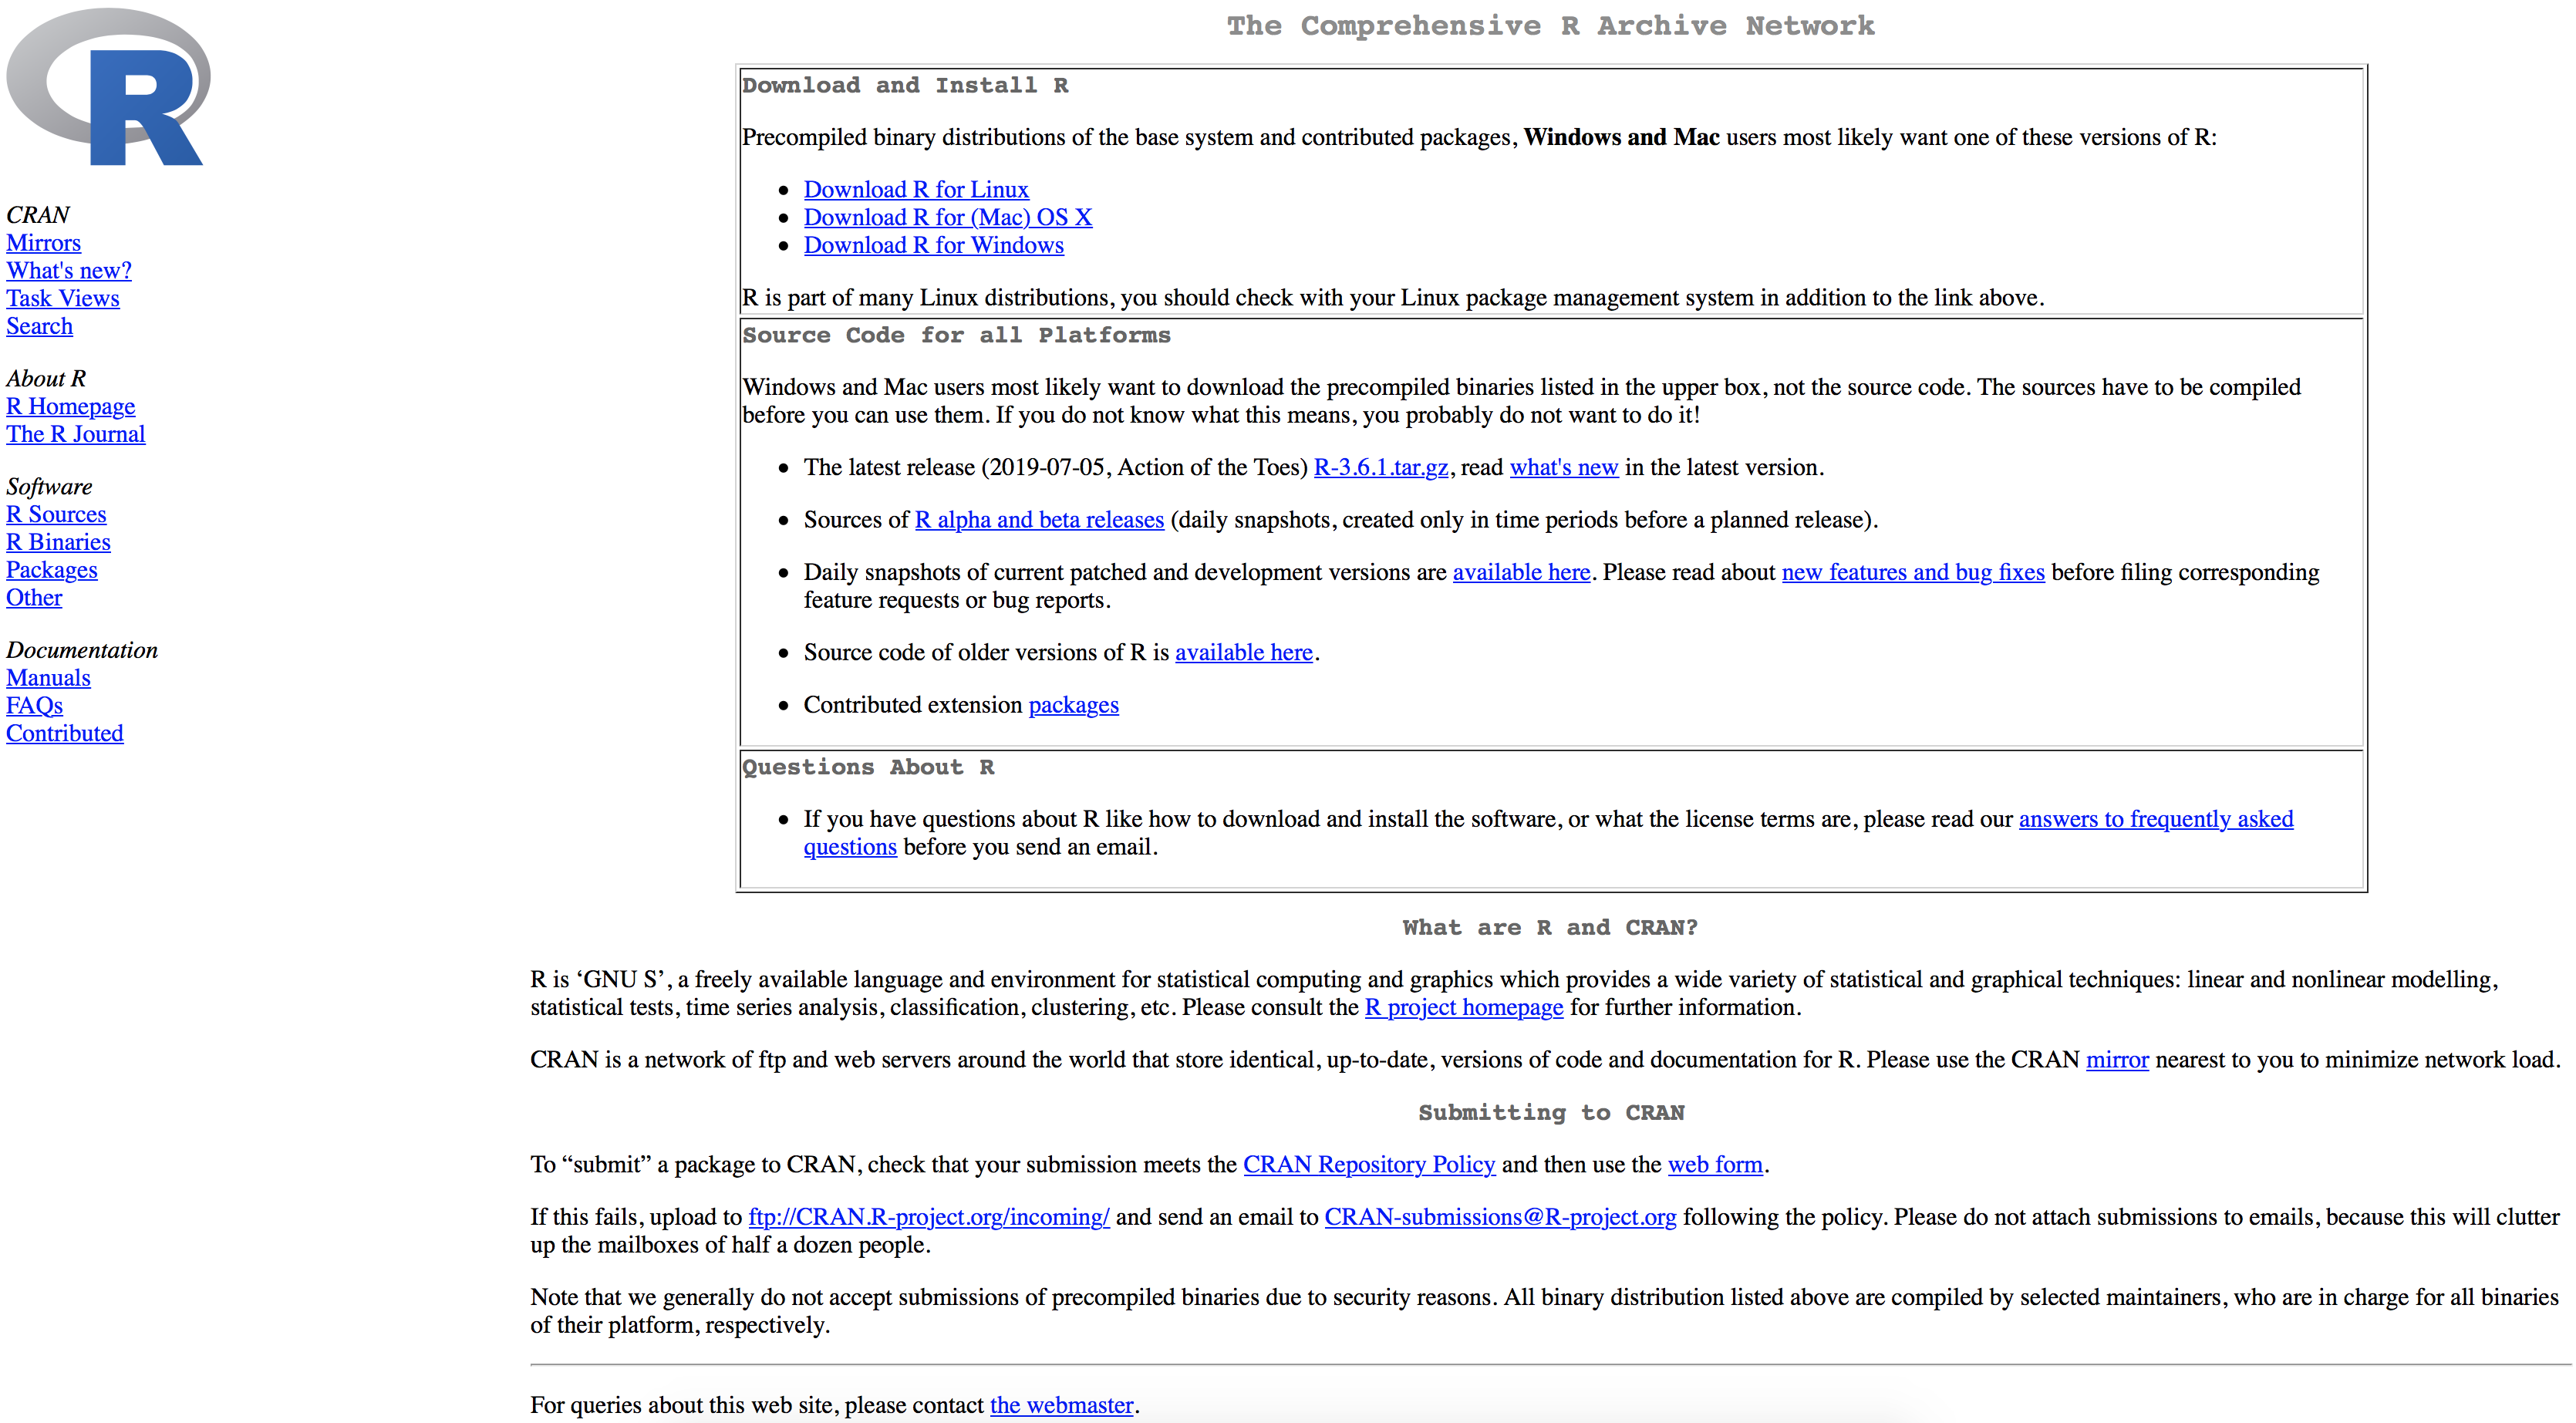
\includegraphics[width=0.9\linewidth]{figures/ch3_cran}
%\caption{The Comprehensive R Archive Network.}
%\label{fig:cran}
%\end{figure}

After installing R, let us immediately install RStudio Desktop (the free version).
Go to \url{https://rstudio.com/products/rstudio/download/#download} and download and run the installer for your computer.
If you open RStudio you should get a screen similar to \reffig{rstudio}.
If this is the first time you open RStudio you probably don't see the top left pane (the scripts),
you can create that pane by creating a new \emph{R Script} via the \emph{file} menu or with the green plus icon in the top left corner. 

\begin{figure}
\centering
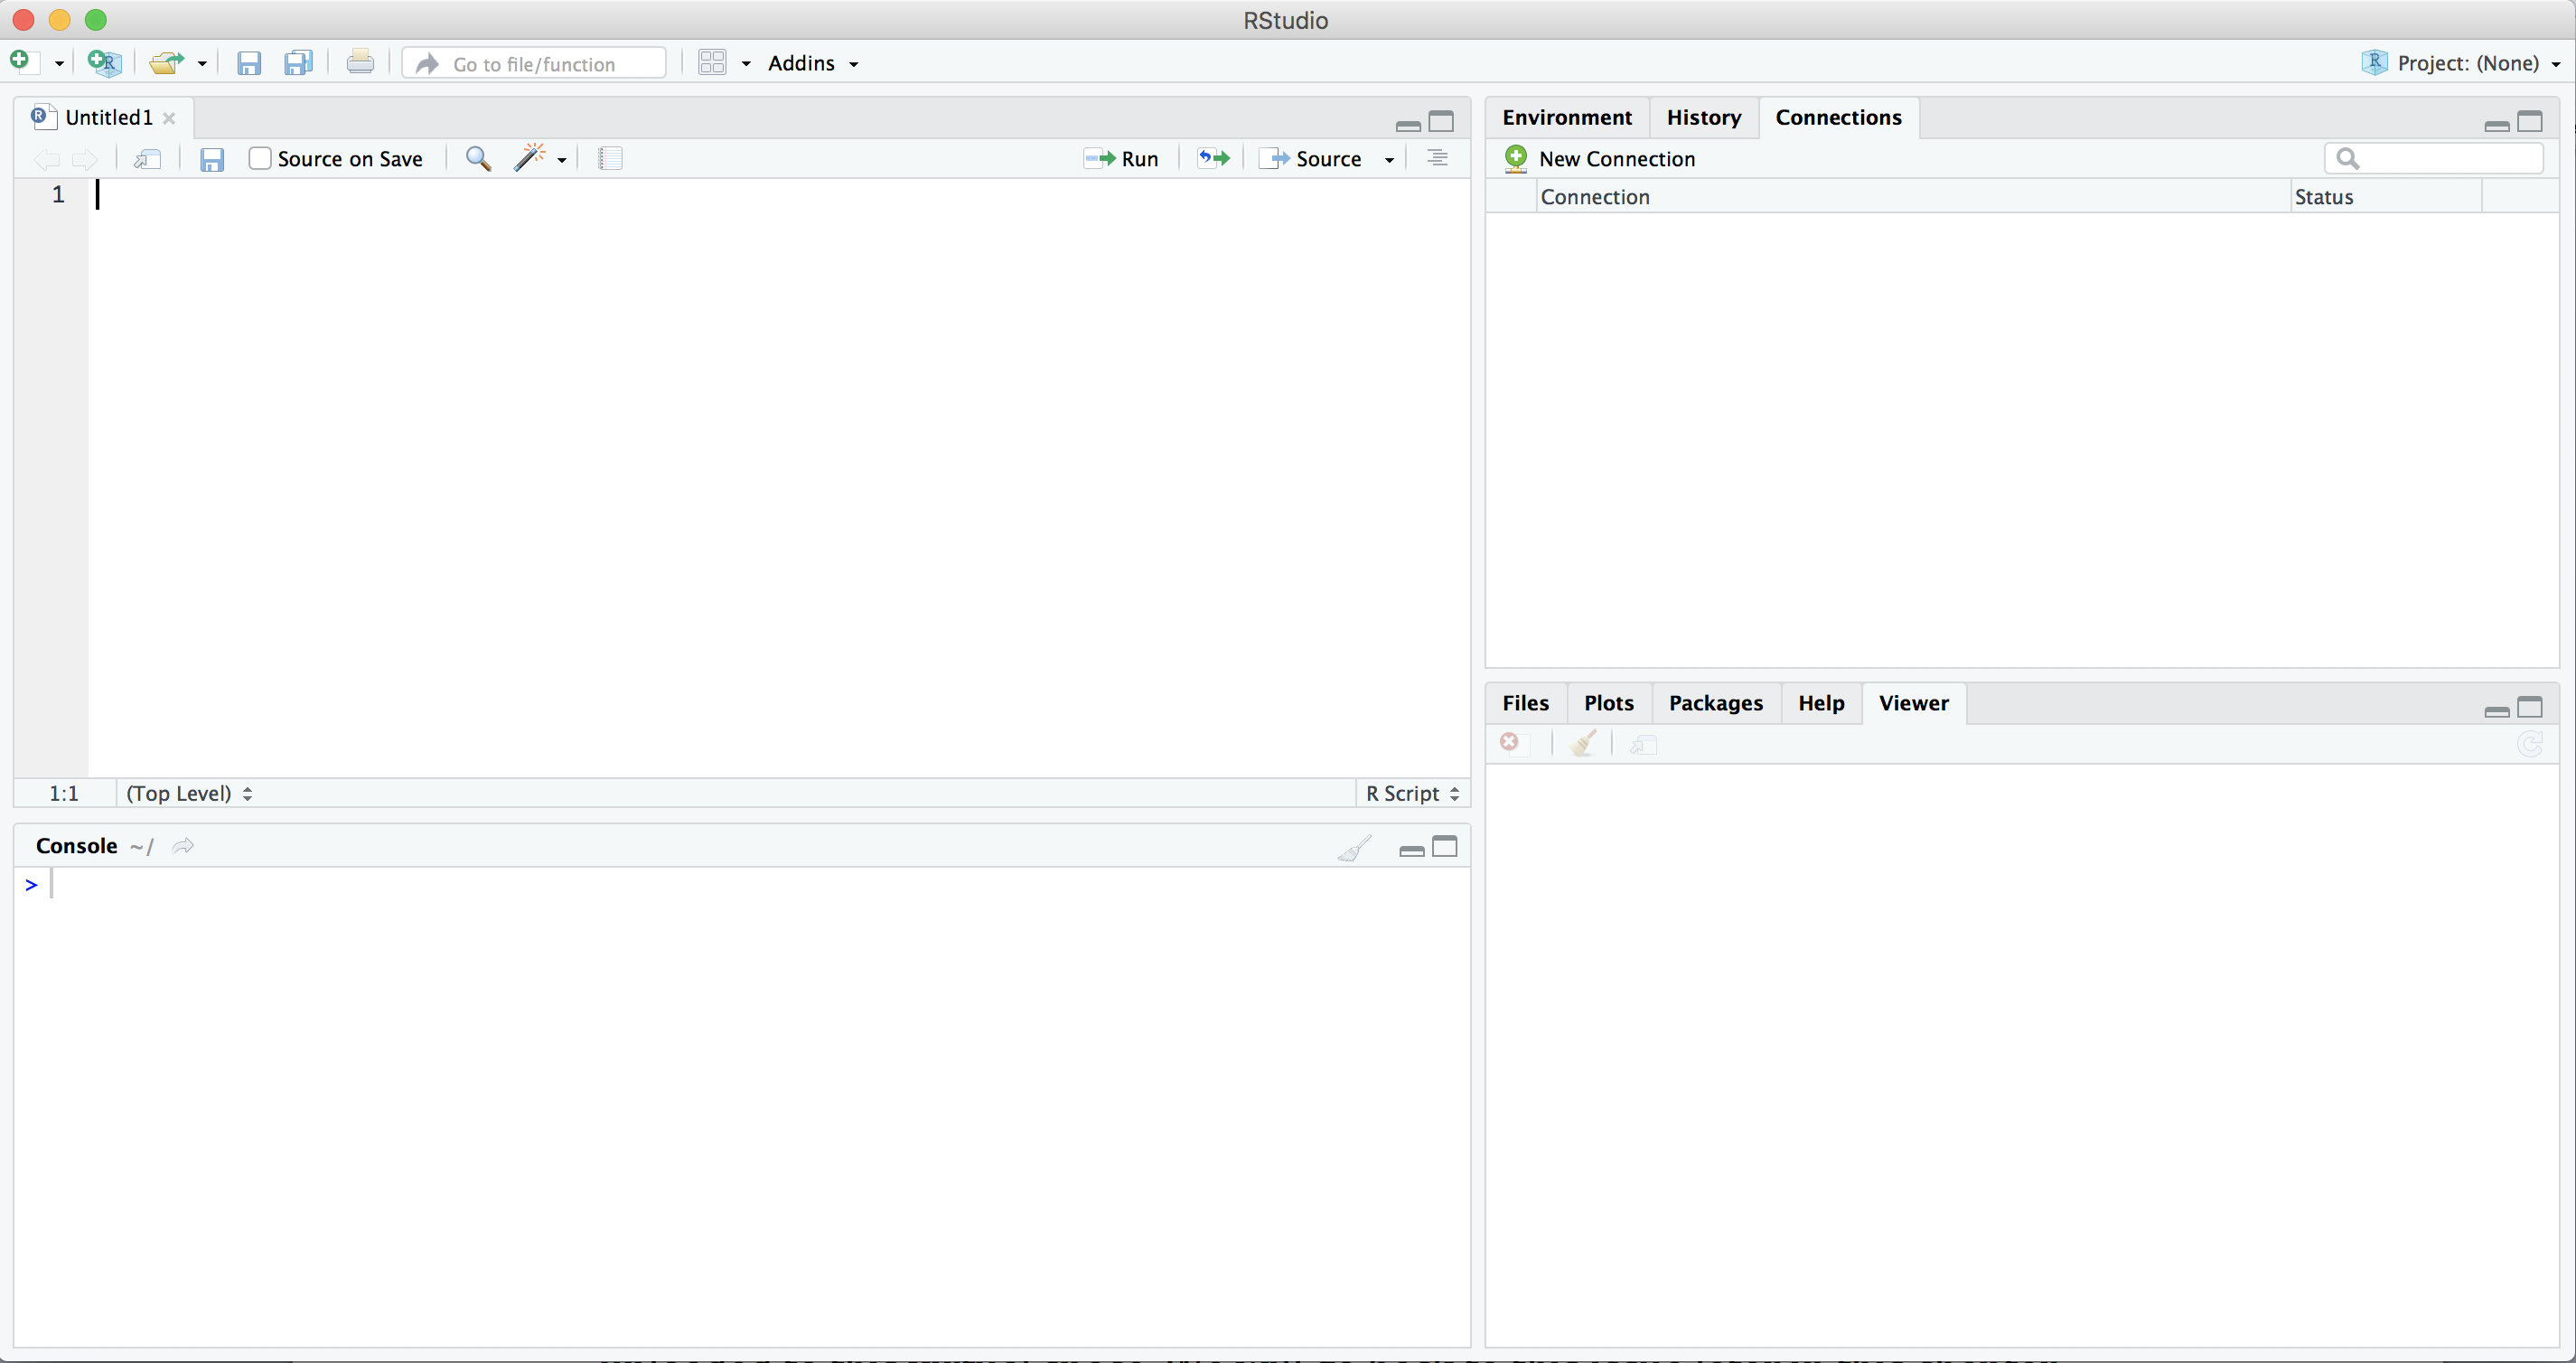
\includegraphics[width=0.9\linewidth]{figures/ch3_r_studio.png}
\caption{RStudio Desktop.}
\label{fig:rstudio}
\end{figure}

Of the four panes in RStudio,
you will probably spend most time in the top left pane, where you can view and edit your analysis \emph{scripts}.
A script is simply a list of commands that the computer should execute one after the other,
for example: open your data, do some computations, and make a nice graph. 

To run a line of code, you can place your cursor anywhere on that line and click the \emph{Run} icon or
press control+Enter.
To try that, type the following into your newly opened script:

\verb|print("Hello world")|

Now, place your cursor on that line and press Run (or control+Enter).
What happens is that the line is copied to the \emph{Console} in the bottom left corner
and executed.
So, the results of your commands (and any error messages) will be shown in this console view.

In contrast to most traditional programming languages,
the easiest way to run R code is line by line.
You can simply place your cursor on the first line,
and repeatedly press control+Enter, which executes a line and then places the cursor on the next line.
You can also select multiple lines (or part of a line) to execute those commands together,
but in general it is easiest to check that everything is going as planned if you run the code line by line.

You can also write commands directly in the console and execute them (by pressing enter).
This can be useful for trying things out or to run things that only need to be run once,
but in general we would strongly recommend typing all your commands in a script and then executing them.
That way, the script serves as a log of the commands you used to analyze your data,
so you (or a colleague) can read and understand how you did the analyses. 

\begin{feature}
  \textbf{RStudio Projects}
  A very good idea to organize your data and code is to work with RStudio Projects.
  In fact, we would recommend you to now create a new empty project for the examples in this book.
  To do this, click on the \emph{Project} button in the top right and select ``New Project''.
  Then, select New Directory and New Project and enter a name for this project
  and a parent folder for the project if you don't want it in your Documents. 
  Using a project means that the scripts and data files for your project are all in the same location
  and you don't need to mess around with specifying the locations of files
  (which will probably be different for someone else or on a different computer).
  Moreover, RStudio remembers which files you were editing for each project,
  so if you are working on multiple project it's very easy to switch between them.
  We recommend creating a project now for the book (and/or for any projects you are working on),
  and always switching to a project when you open RStudio
\end{feature}


On the right side of the RStudio workspace you will find two additional
windows. In the top right pane there are two or more tabs:
\emph{environment} and \emph{history}, and depending on additional
packages you may have installed there may be some more.  In
\emph{environment} you can manage your workspace (the set of elements
you need to deploy for data analysis) and have a list of the objects
you have uploaded to it. You may also import datasets with this tool.
In the \emph{history} tab you
have an inventory of code executions, which you can save to a file, or
move directly to console or to an R document.

Note that in the environment you can save and load your ``workspace'' (all data in the computer memory).
However, relying on this functionality is often not a good idea: it
will only save the state of your current session, whereas you most
likely want to save your R syntax file and/or your data instead.
If you have your raw input data (e.g., as a csv file, see \refchap{filetodata})
and your analysis script, you can always
reproduce what you have been doing. If you only have a snapshot of
your workspace, you know the state in which you arrived, but cannot
necessarily reproduce (or change) how you got there.

In the bottom right pane there are five additional useful tabs.
In \emph{files} you can explore
your computer and manage all the files you may use for the project,
including importing datasets. In \emph{plots}, \emph{help} and
\emph{viewer}, you can visualize the  outputs, figures, documentation
and general outcomes, respectively, that you have executed in your
script. Finally, the tab for \emph{packages} will be of great
utility since it will let you install or update packages from CRAN or
even from a file saved on your computer with a friendly interface.

\subsection{Installing Python and Jupyter Notebook}

Python is an object-orientated programming language
and it is probably the favorite language of computational and data
scientists in all disciplines around the world.
There are different releases of Python, but the biggest difference used to be between Python 2 and Python 3.
Fortunately, you will probably never need to install or use Python 2, and in fact, since January 2020 it is no longer supported.
Thus, you can just use any recent Python 3 version for this book.
When browsing through questions on online fora such as Stackoverflow or reading other people's code on Github (we will talk about that in \refchap{worldcode}), you still may come across legacy code in Python 2. Such code usually does not run directly in a Python 3 interpreter, but in most cases, only minor adaptions are necessary to make it work.

We will install and run Python and Jupyter Notebook using a \concept{terminal} or command line interface.
This is a tool that is installed on all computers that allows you to give commands to the computer directly.
First, create a project folder for this book using the File Explorer (Windows) or Finder (MacOS).
Then, on Windows you can shift + Right click that folder and select ``Open command Window here''.
On MacOS, after navigating to the folder you just created, you click on ``Finder'' in the menu at the top of the screen, then on ``Services'', then on ``New Terminal at Folder.''
In both cases, this should open a new window (usually black or gray) that allows you to type commands.

Note that on most computers, Python is already installed by default.
You can check this by typing the following the command in your terminal:

\begin{verbatim}
python3 --version
\end{verbatim}

On some versions of Windows, you may need to use \verb|py| instead of \verb|python3|:
\begin{verbatim}
py --version
\end{verbatim}

In either case, the output of this command should be something like \verb|Python 3.8.5|.
If \verb|python --version| also returns this version, you are free to use either command
(but on older systems \verb|python| can still refer to Python 2, so make sure that you are using Python 3 for this book!).

If Python is not installed on your system, go to \url{https://www.python.org/downloads/windows/} or \url{https://www.python.org/downloads/mac-osx/} and download and install the latest stable release (which at the time of writing is \verb|3.9.0|).%
\footnote{For linux, install python3 and pip using your package manager. For example, on ubuntu you can run \texttt{sudo apt install python3-pip}}
After installing it, open a terminal again and run the command above to verify that it is installed correctly.

Included in any recent Python install is \concept{pip}, the program that you will use for installing Python packages.
You can check that pip is installed correctly by typing the following command on your terminal:

\begin{verbatim}
pip3 --version
\end{verbatim}

Which should report something like \texttt{pip 20.0.2 from ... (python 3.8)}.
Again, if \verb|pip| reports the same version you can also use it instead of pip3.
On some systems \verb|pip3| will not work, so use \verb|pip| in that case
(but make sure to check that it points to Python 3).

\paragraph{Installing Jupyter Notebook}
Next, we will install Jupyter Notebook, which you can use to run all the examples in this book
and is a great environment for developing Python data analysis scripts.
Jupyter Notebooks (which are also included in IDE JupyterLab if you installed that), 
are run as a web application
that allows you to create documents that contain code and inline text fragments.
 One of the nicest things about 
the Jupyter Notebook is that the code is inserted in fields (so-called ``cells'') that you
can run one by one, getting its respective output, which added to the
designed narrative text will make your script more clean and
reproducible. You can also add formatted text blocks (using a simple formatting language called \concept{Markdown})
to explain to the reader what you are doing. In \refsec{practices}, we will address
notebooks again as a good practice for a computational scientist.

You can install Jupyter notebook directly using pip using the following command
(executed in a terminal):

\begin{verbatim}
pip3 install jupyter-notebook
\end{verbatim}

Now, you can run Jupyter by executing the following command on the terminal:

\begin{verbatim}
jupyter notebook
\end{verbatim}

This will print some useful information, including the URL at which you can access the notebook.
However, it should also directly open this in a browser (e.g. Chrome) so you can directly start working. 
In your browser you should see the Jupyter main screen similar to the middle window in \reffig{jupyter}.
Create a new notebook by clicking on the \emph{New} button in the top right and selecting Python 3.
This should open a window similar to the bottom window in \reffig{jupyter}.

\begin{figure}
  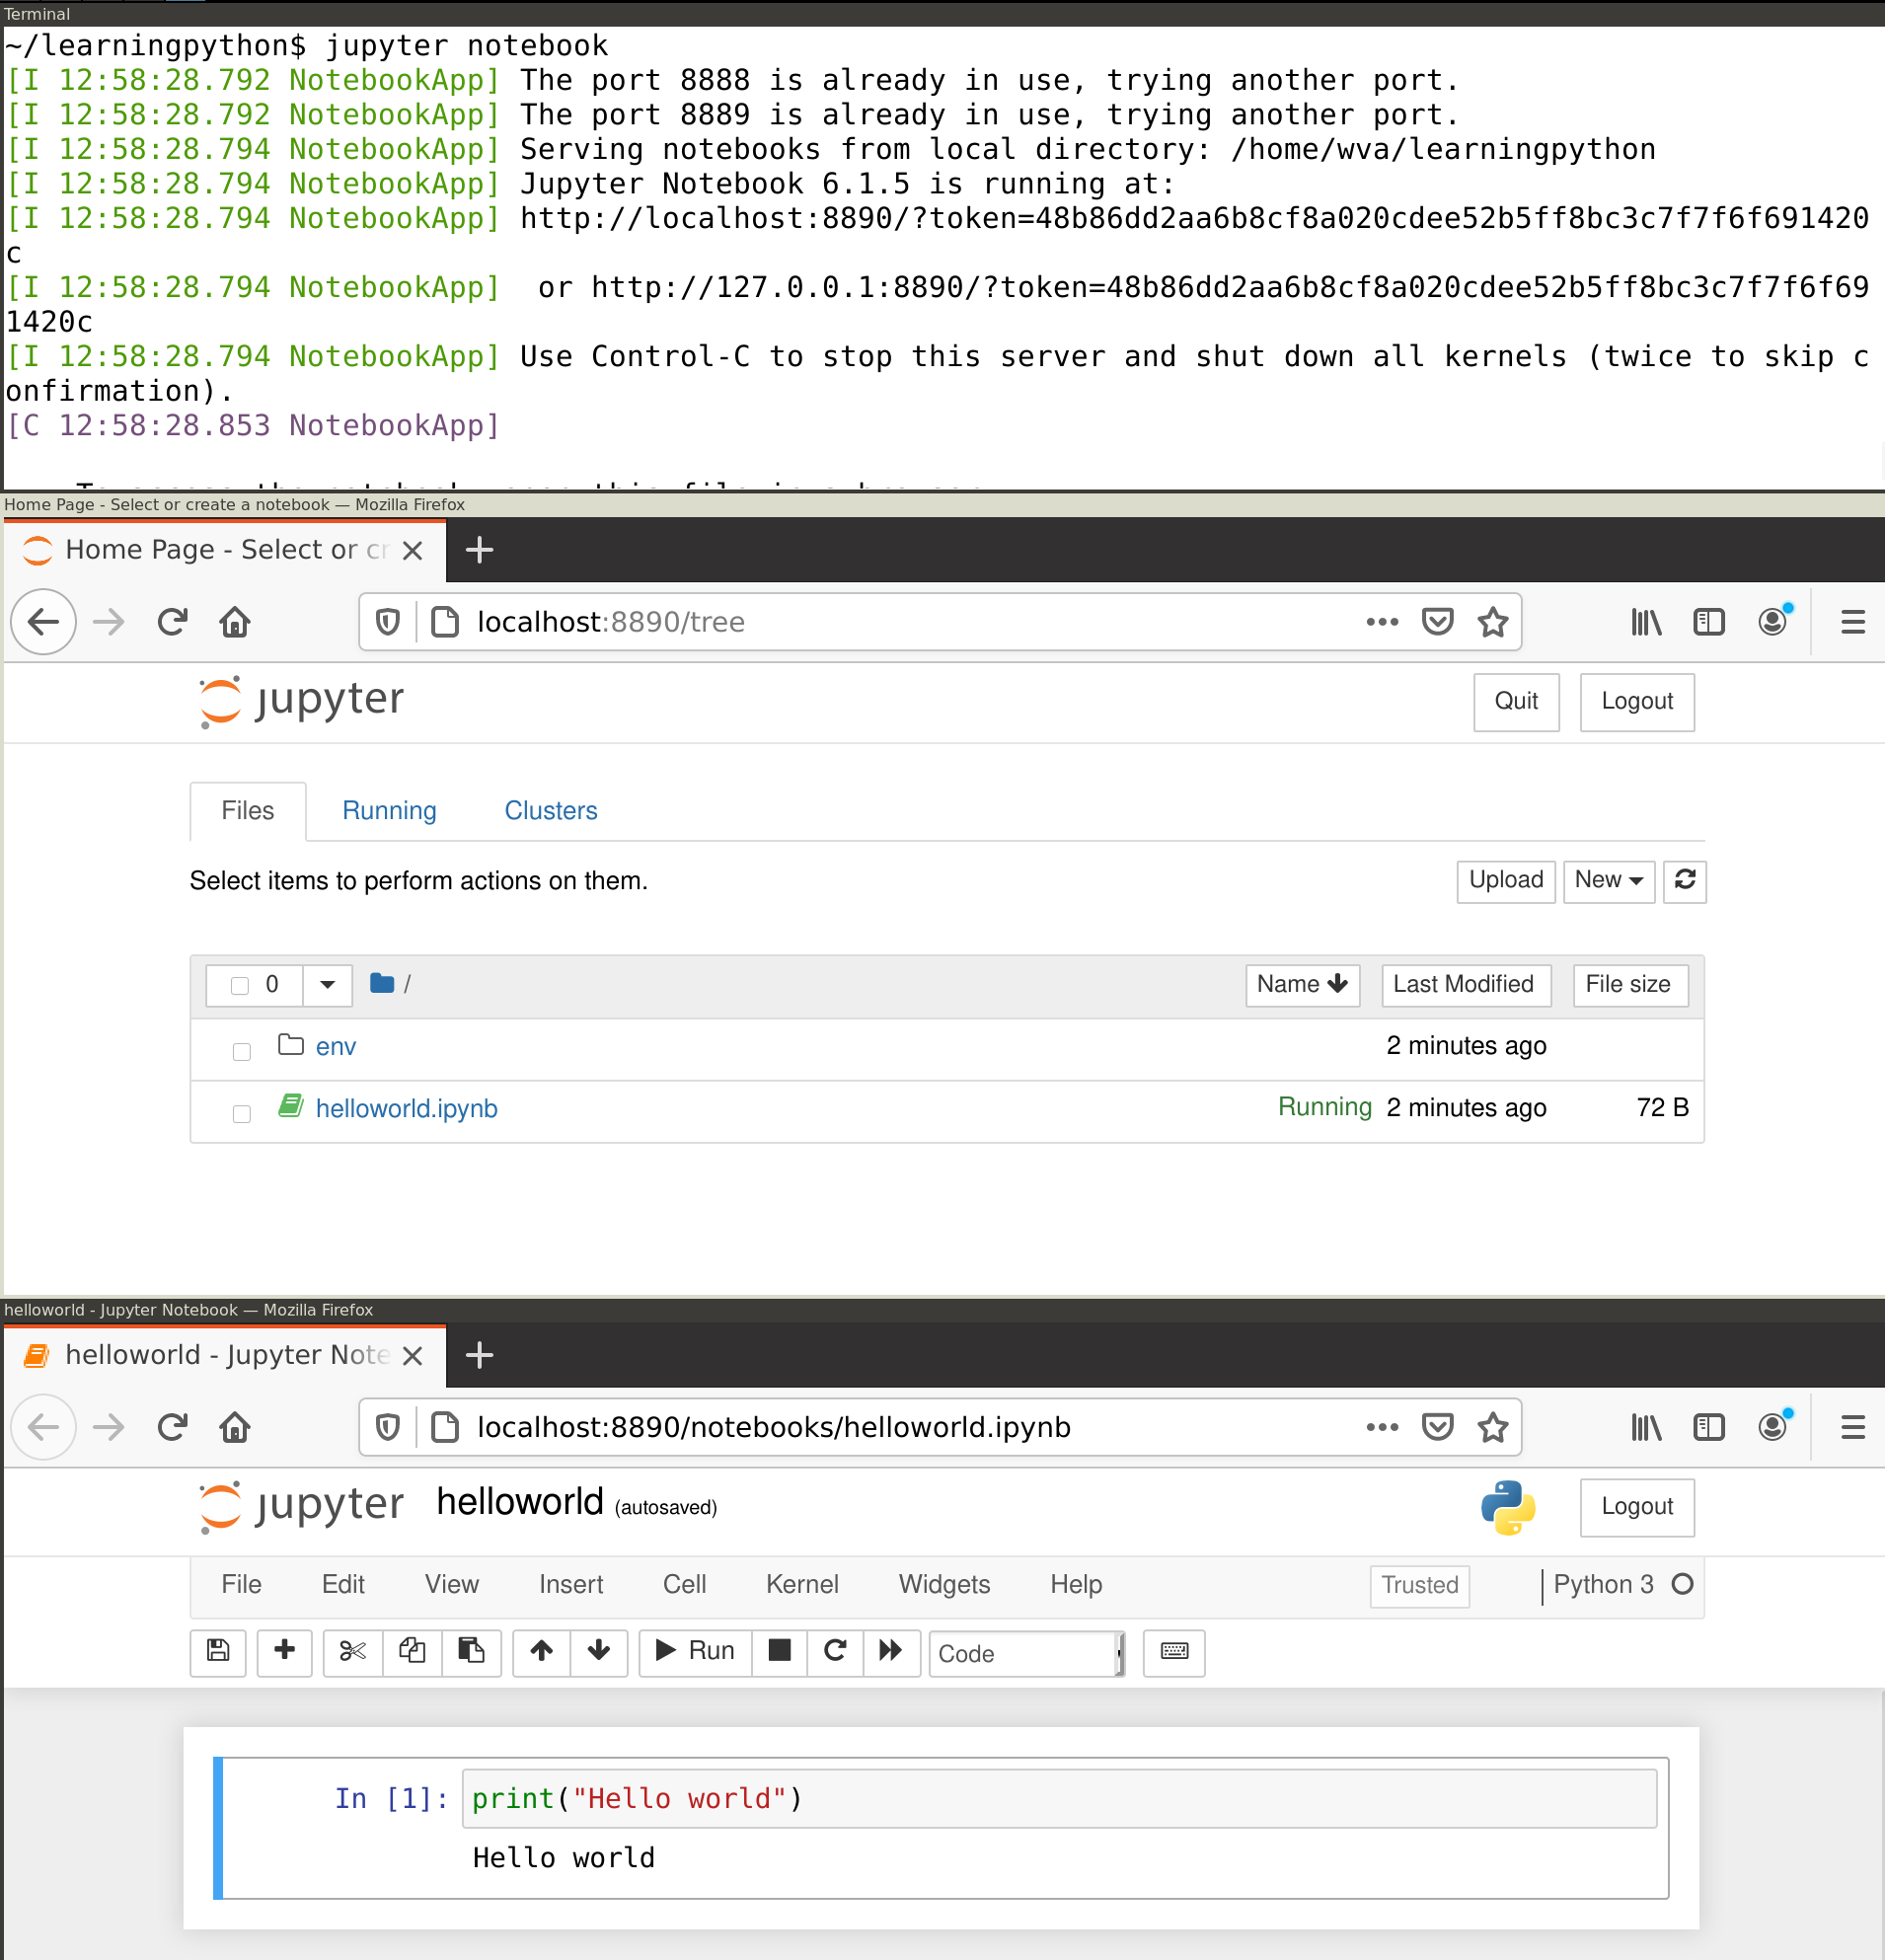
\includegraphics[width=\textwidth]{figures/jupyter.png}
  \caption{Jupyter Notebook.}\label{fig:jupyter}
\end{figure}

In Jupyter, code is entered into cells.
First, type \verb|print("Hello World")| into the empty cell next to the \verb|In [ ]:| prompt.
Then, click the Run button or press control+Enter. This should execute your command and display
the text \verb|"Hello World"| in the output area right below the input cell.
Note that you can create more cells using the plus icon or with the insert menu.
You can also set the cell type via the Cell menu: select code for analysis scripts (which is the default),
or Markdown for text fragments, which can be used to explain the code and/or interpret the results.

\section{Installing Third-Party Packages}

The \index{print}\texttt{print} function used above is included automatically when you start R or Python.
Many functions, however, are included in separate \concept{packages} (also known as \concept{libraries} or \concept{modules}), which are
generally collections of commands for a certain task or activity.

Although both R and Python come pre-installed with many useful \concept{packages},
one of the great things of both languages is that they have a very active community that continuously develops, improves, and publishes new packages.
Throughout this book, we will be using such third-party packages for a variety of tasks, from data wrangling and visualization to text analysis.
For example, we will use the R package \emph{tidyverse} and the Python packages \emph{pandas} for data wrangling.

To install these packages on your computer, run the following commands:
(Note: if you are using Anaconda, replace \ttt{pip3 install} by \ttt{conda install})  

\begin{tcbraster}[raster columns=2,raster equal height=rows,raster valign=top]
   \codex[caption=Installing a package from Jupyter]{chapter01/ch01install.py}
   \codex[caption=Installing a package in R]{chapter01/ch01install.r}
\end{tcbraster}


These commands will automatically fetch the package from the right repository\footnote{Similar to the App Store or Play Store, both R and Python have a centralized repository for third party packages.  For R, this is the Comprehensive R Archive Network (CRAN) encountered earlier,
    while for Python this is the Python Package Index (PyPI) accessed by \verb|pip|.  Normally, all packages in these repositories are open source and safe to install.} and install them on your computer. This can take a while, especially for large packages such as tidyverse.
Fortunately, this only needs to be done once.
Every time time you use a package, you also need to \emph{activate} it using the \index{import}\texttt{import} (Python) or  \index{library}\texttt{library} (R) command.

In general, whenever you get an error \texttt{No module named 'pandas'} (Python) or \texttt{there is no package called ‘tidyverse’},
you can just install the package with that name using the code listed above.
If you get an error such as \texttt{name 'pandas' is not defined} (Python) or \texttt{object 'ggplot' not found} (R),
it is quite possible you forgot to activate the package that includes that function. 


\begin{feature}
\textbf{Packages used in each chapter}\\
Some packages, like the \emph{tidyverse} (R) and \emph{pandas} (Python) packages for data handling are used in almost every chapter.
Many chapters also introduce specific packages such as \emph{igraph}/\emph{networkx} for network analysis in \refchap{network}.
To make it easy to keep track of the packages needed for each chapter,
every chapter that includes code in this book starts with a note like this that gives an overview of the main packages introduced in that chapter.
It also includes the code needed to install these packages, which of course is only needed if you didn't install these packages before.
Note again that if you are using Anaconda for Python,
you should replace \ttt{!pip3 install} by \ttt{!conda install} in that code. On some systems, you may need to use \ttt{!pip install} instead of \ttt{!pip3 install}.

These notes also includes a code block to import all the packages used for that chapter,
which you need to run every time you use examples from that chapter.
\end{feature}

%\section{Installing R and Python}
\label{sec:installing}

R and Python are the most popular programming languages that data
scientists and computational scholars have adopted to conduct their
work (see \refchap{introduction}). While many develop a preference
for the one or the other language, chances are good that you
will ultimately switch back and forth between them, depending on
the specific task at hand and the project you are involved in.

Before you can start with analysing data and communication in Python or R,
you need to install these languages on your computer.
Both Python and R are open source and completely free to download and use.
Although there are various web-based services on which you can run code for both languages
(such as google Colab or RStudio Cloud),
it is generally better to install them on your own computer.

After installing Python or R, you can execute code in these languages, but you also want a nice
\concept{Integrated Development Environment (IDE)} to develop your data analysis scripts. 
For R we recommend RStudio, which is free to install and is currently the most popular environment for working with R.
For Python we recommend starting with JupyterLab, which is a web-based environment for writing and running python code.
All of these tools are available and well documented for Windows, MacOS, and Linux. 
After explaining how to install R and Python, there is a very important section on installing packages.
If you plan to only use either R or Python (for now), feel free to skip the part about the other language.

Note that If you are writing longer Python programs you probably want to install a desktop IDE (Integrated Development Environment)
as well.
We recommend PyCharm\footnote{\url{https://www.jetbrains.com/pycharm/}} for this, which has a free version that has everything you need, and the premium version is also free for students and academic or open source developers.
See their website for download and installation instructions.


\begin{feature}\textbf{Anaconda}. An alternative to installing 
  R, Python, and optional libraries separately and as you need them
  (which we will explain in this chapter) is to install the so called
  Anaconda distribution, one of the most used and extensive platforms
  to perform data science. Anaconda is free and open-source, and is
  conceived to run Python and R code for data analysis and machine
  learning. Installing the complete Anaconda Distribution on your
  computer\footnote{\url{https://www.anaconda.com/distribution/\#download-section}}
  provides you with everything that you need to follow the examples in
  this book and includes development environments such as Spyder,
  Jupyter, and RStudio. It also includes a large set of pre-installed
  packages often used in data science and an own package manager,
  \pkg{conda}, which will help you to install and update other
  libraries or dependencies. In short, Anaconda bundles the almost all
  important software to perform computational analysis of
  communication.

  So, should you install Anaconda, or should you
  install all software separately as outlined in this chapter? It
  depends. On the pro side, you just have everything installed at once and do
  not have to worry about dependencies (e.g., Windows users ususally
  do not have a C compiler installed, but some packages may need
  it). On the con side, next to that it is huge and also installs many
  things you don not need, you essentially get a non-standard
  installation, in which programs and packages are stored in different
  locations than you (or your computer) may expect. As many computers
  actually already \emph{have} Python installed (even though you may
  not know it), you also end up in a possibly confusing situation
  where it may be unclear which version you are actually running, or
  for which version you installed a package.
  For this reason, our recommendation is to not use Anaconda unless
  it is already installed or you have a specific reason to do so
  (for example, if your professor requires you to use it).
\end{feature}

\subsection{Installing R and RStudio}

Firstly, we will install R and its most popular IDE RStudio, and we
will learn how to install additional packages and how to run a
script. R is an object-based programming language
orientated to statistical computing that can be used for most of the
stages of computational analysis of communication.  If you are
completely new to R, but familiar with other popular
statistical packages in social sciences (such as SPSS or STATA), you
will find that you can perform in R many already-known statistical
operations. If you are not familiar with other statistical packages,
do not panic, we will guide you from the very beginning. Unlike
many traditional software that requires just one complete and initial
installation, when working with R, we will first install the raw
programming language and then we will keep on installing additional
components during all of our journey. It might sound cumbersome, but
in fact it will make your work more powerful and flexible, since you
will be able to choose the best way to interact with R and especially
you will select the packages that are suitable for your project.

Now, let's install R.
The easiest way is to go to the RStudio CRAN page at \url{https://cran.rstudio.com/}.
\footnote{\concept{CRAN}, short for Comprehensive R Archive Network, is a network
  of web sites on which R itself and various R packages are hosted.}
Click on the link for installing R for your operating system, and
install the latest version.
If you use Linux, you may want to install R via your package manager.
For Ubuntu linux, it is best to follow the instructions on \url{https://cran.r-project.org/bin/linux/ubuntu/}.

%\begin{figure}
%\centering
%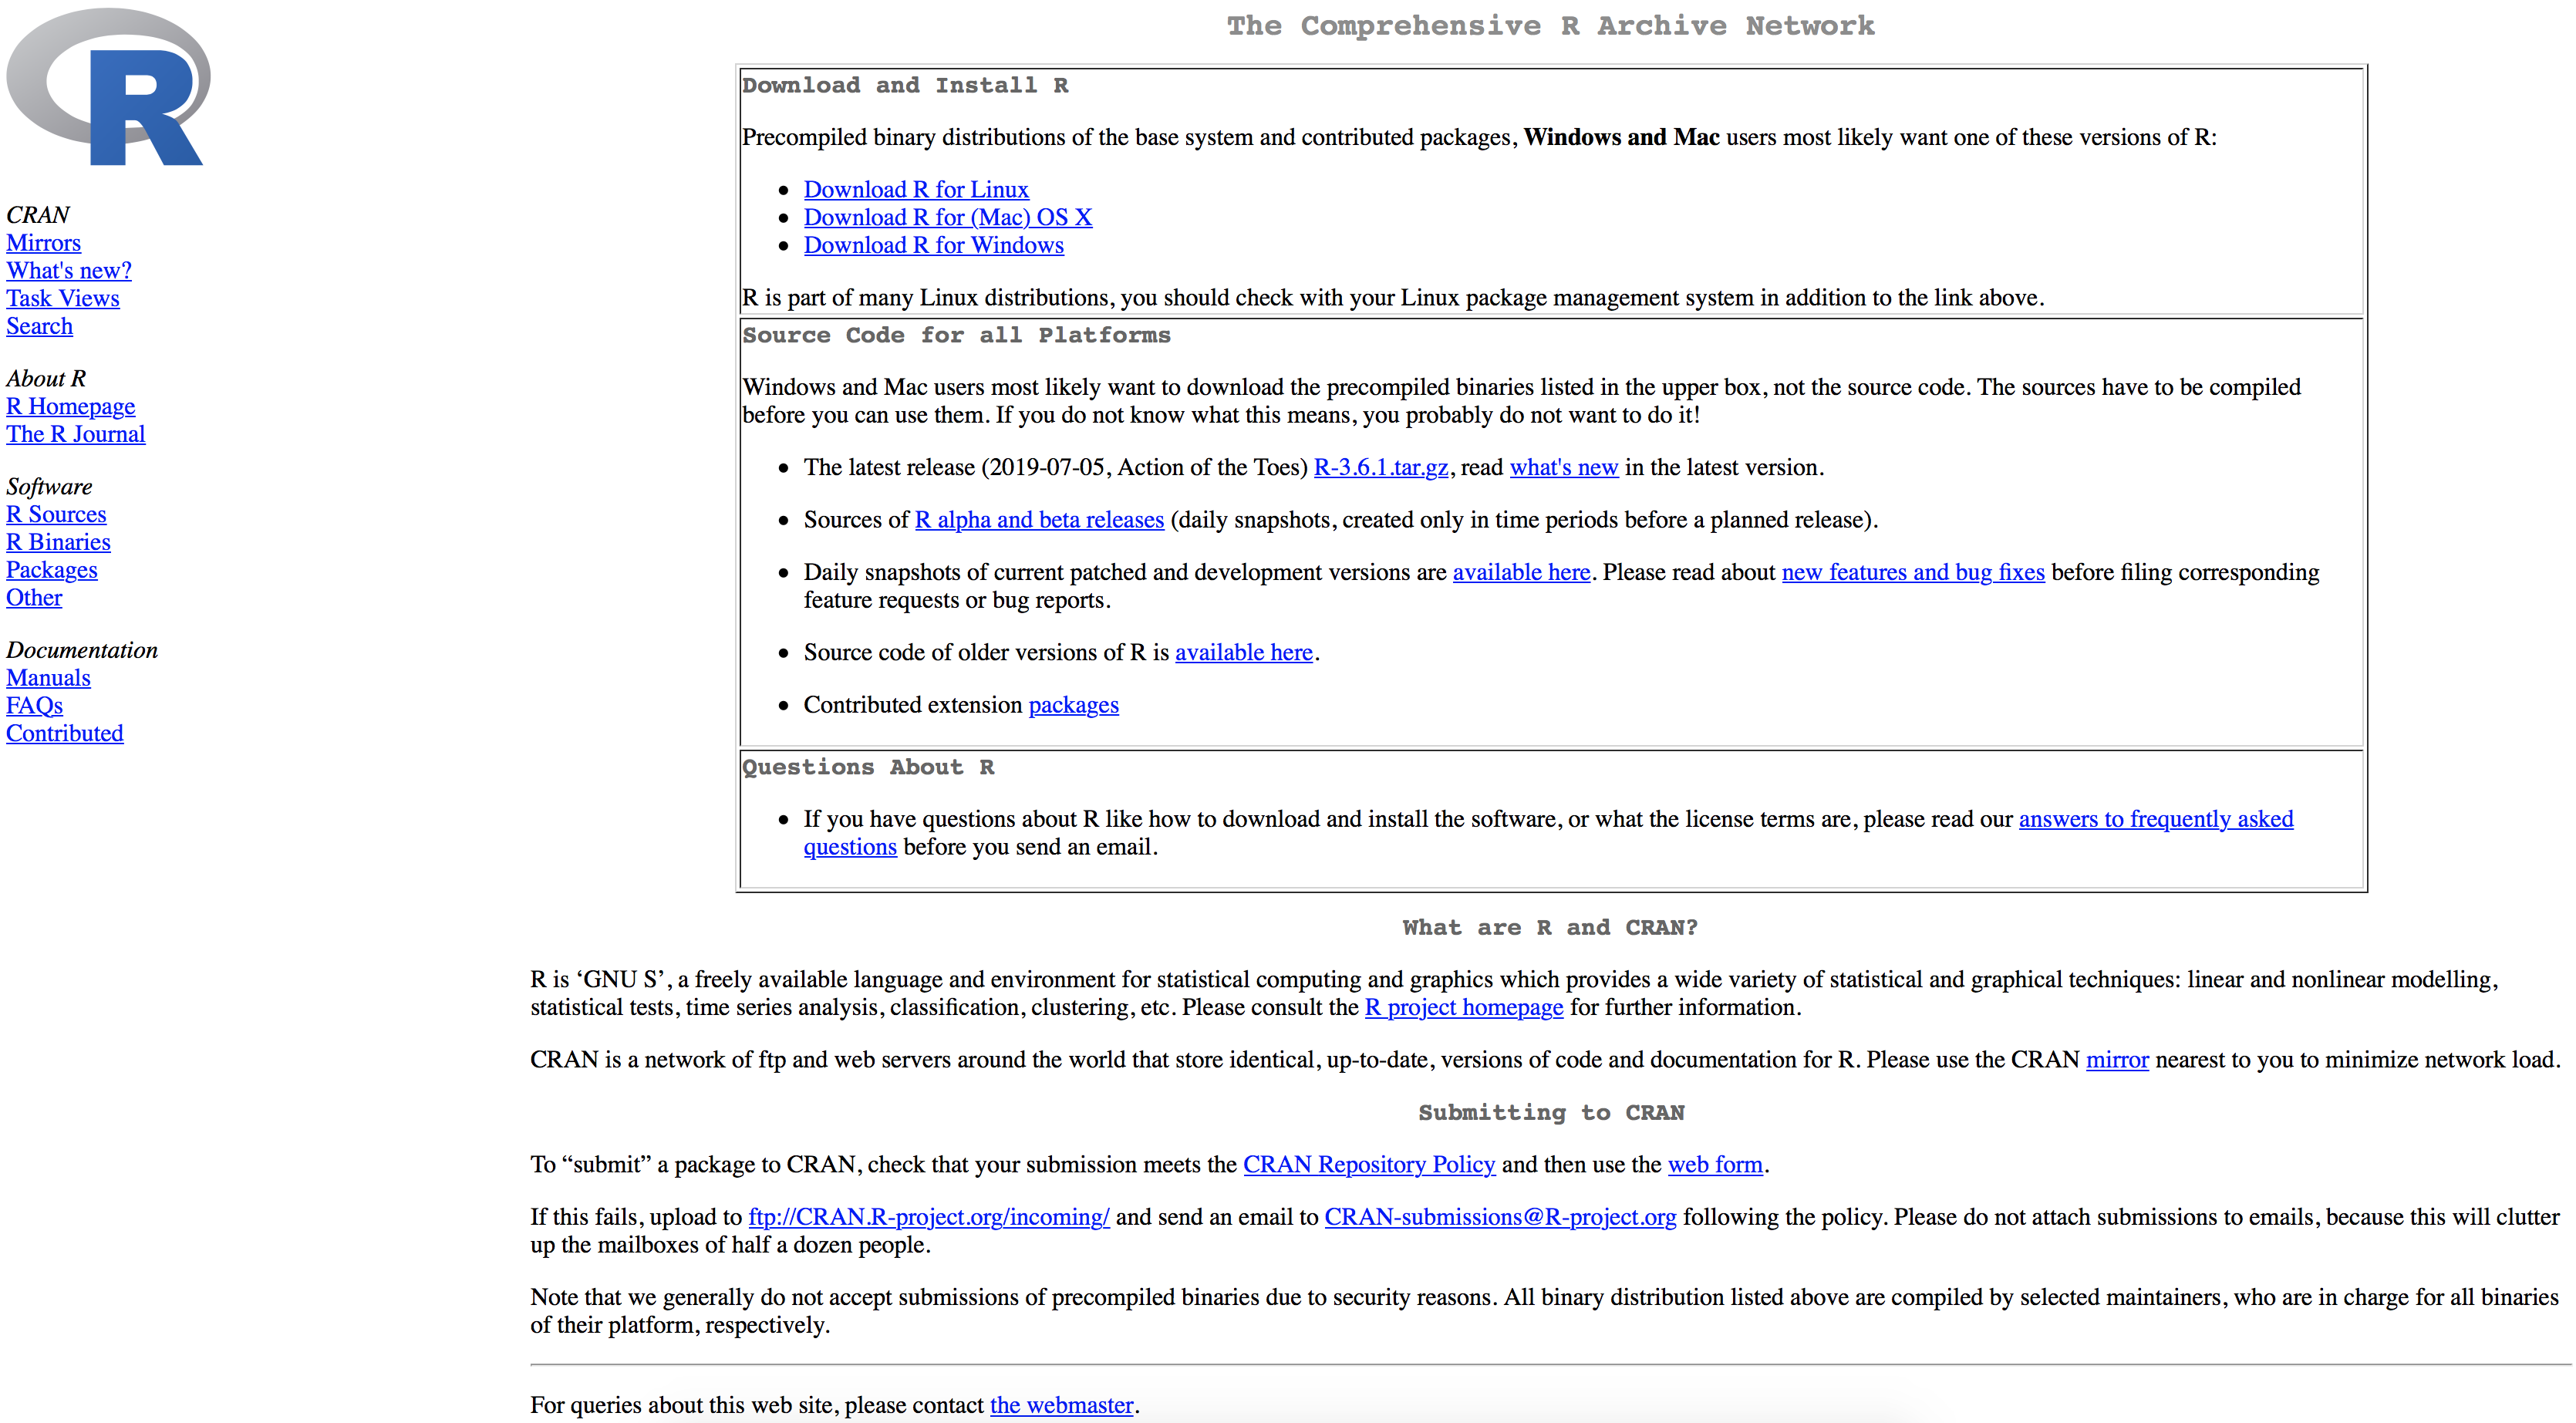
\includegraphics[width=0.9\linewidth]{figures/ch3_cran}
%\caption{The Comprehensive R Archive Network.}
%\label{fig:cran}
%\end{figure}

After installing R, let's immediately install RStudio Desktop (the free version).
Go to \url{https://rstudio.com/products/rstudio/download/#download} and download and run the installer for your computer.
If you open RStudio you should get a screen similar to \reffig{rstudio}.
If this is the first time you open RStudio you probably don't see the top left pane (the scripts),
you can create that pane by creating a new \emph{R Script} via the \emph{file} menu or with the green plus icon in the top left corner. 

\begin{figure}
\centering
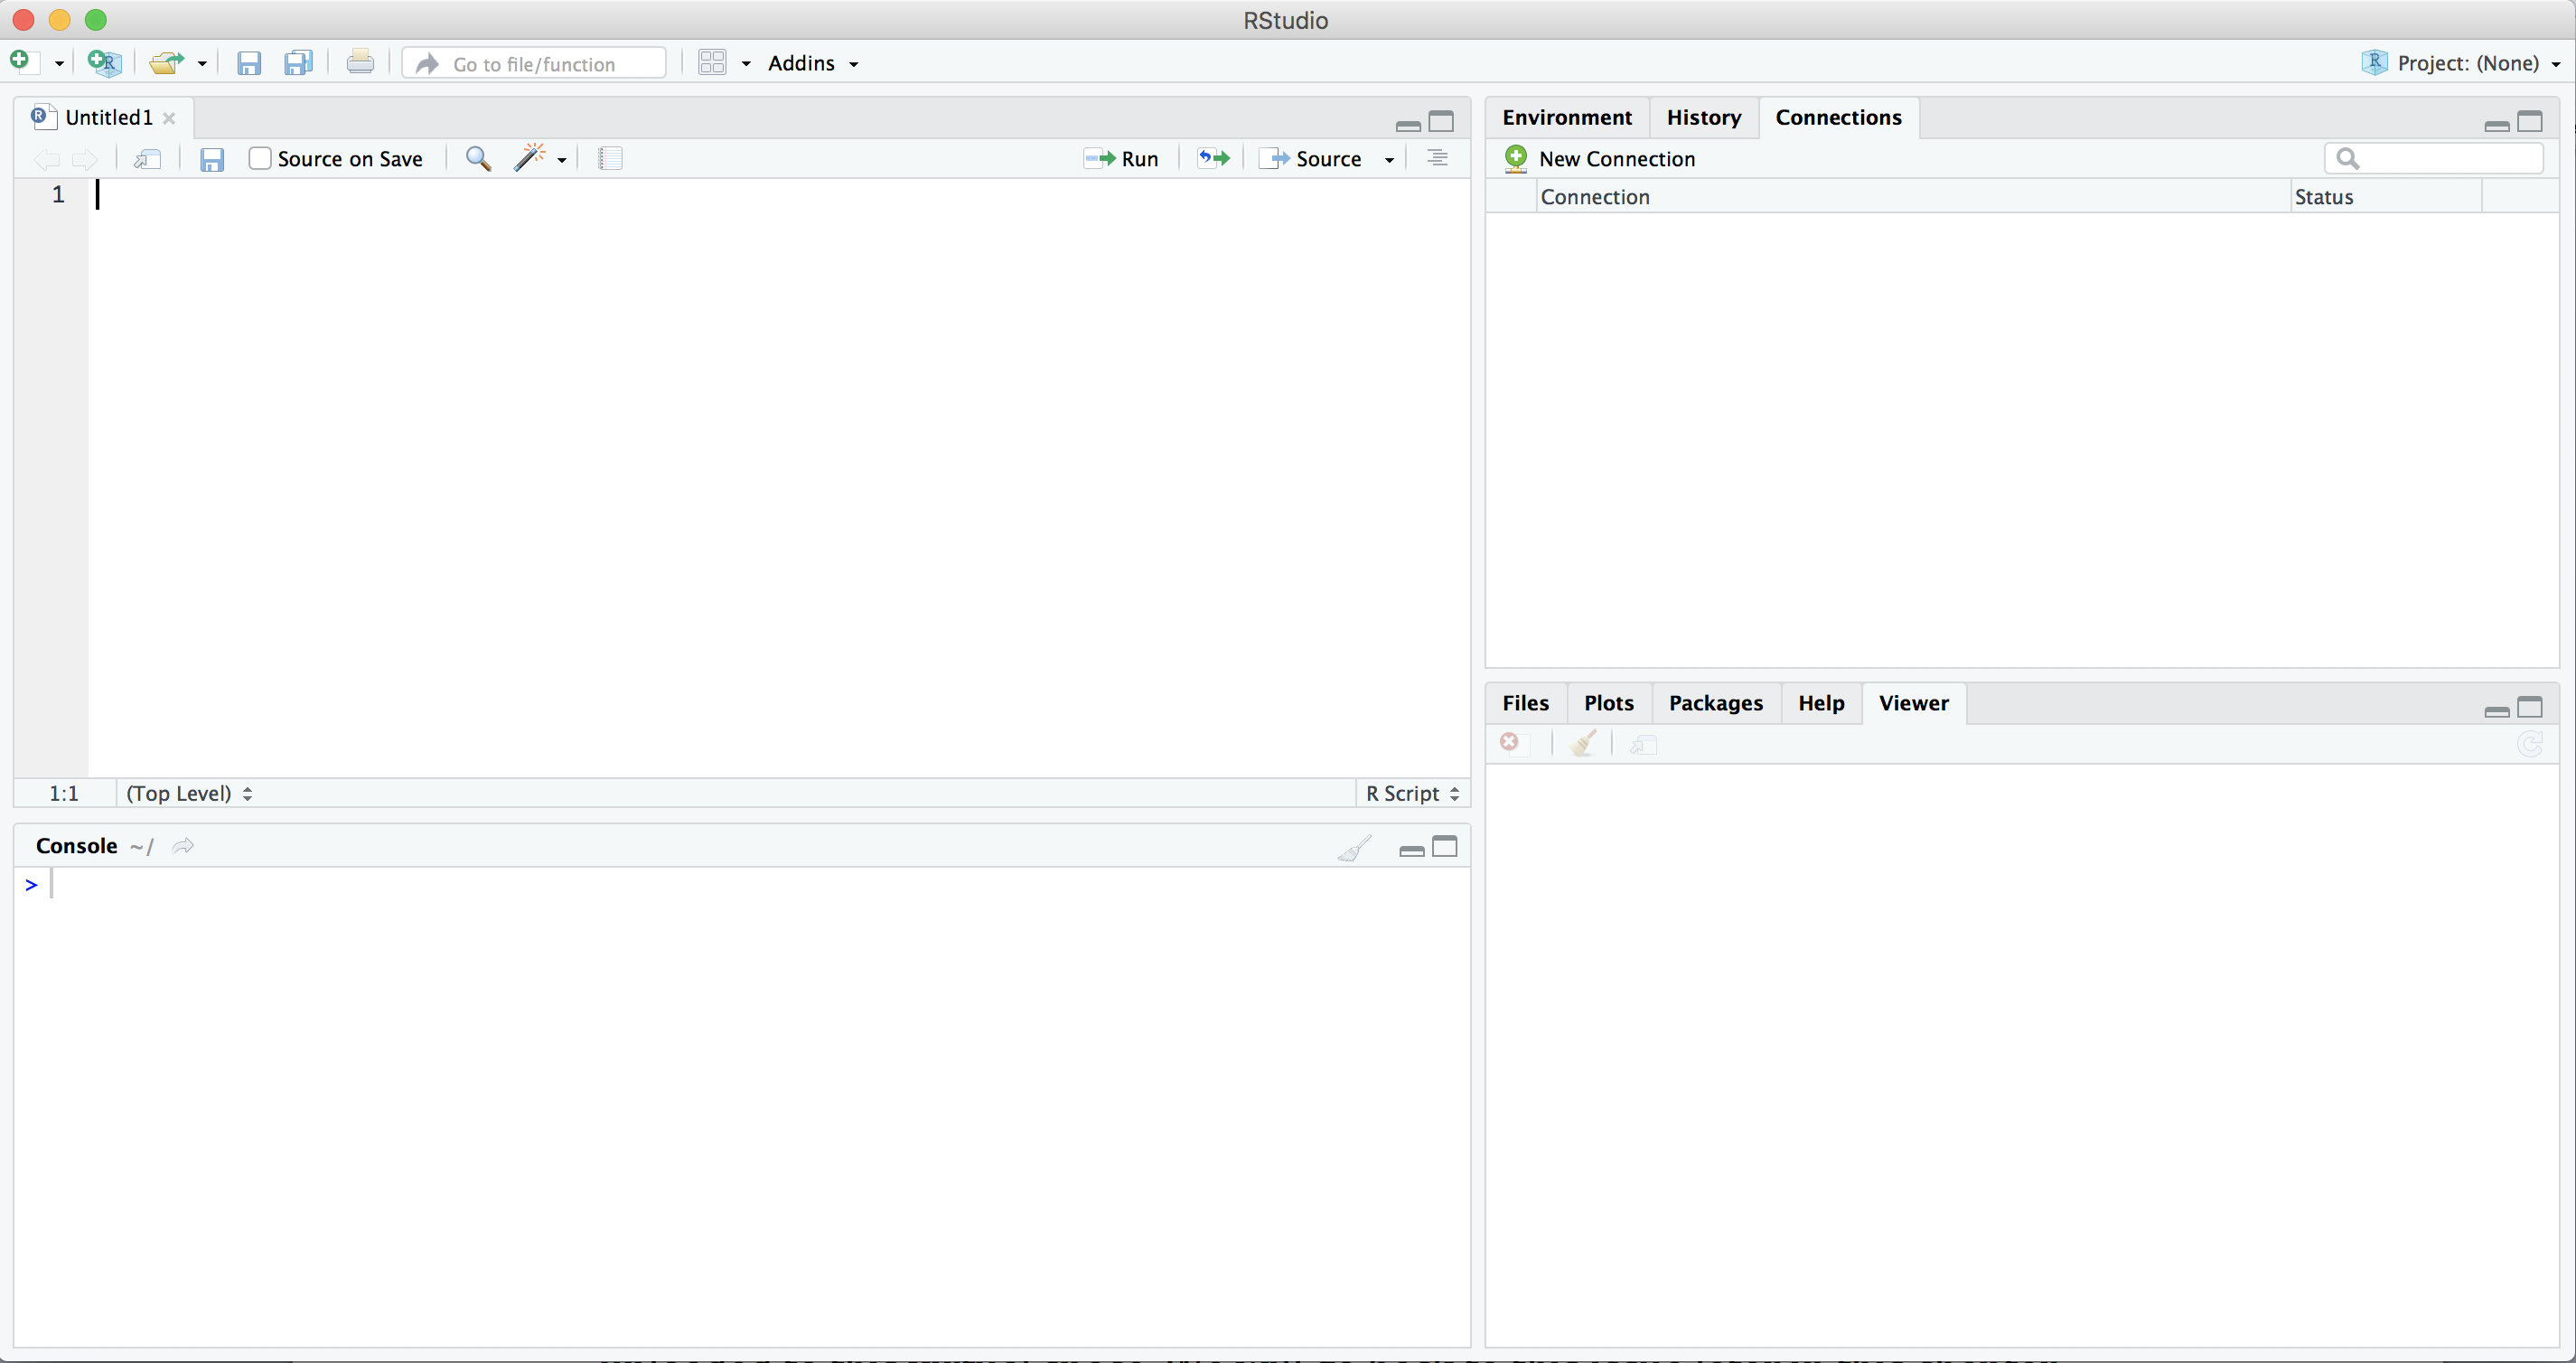
\includegraphics[width=0.9\linewidth]{figures/ch3_r_studio}
\caption{RStudio Desktop}
\label{fig:rstudio}
\end{figure}

Of the four panes in RStudio,
you will probably spend most time in the top left pane, where you can view and edit your analysis \emph{scripts}.
A script is simply a list of commands that the computer should execute one after the other,
for example to open your data, do some computations, and make a nice graph. 

To run a line of code, you can place your cursor anywhere on that line and click the \emph{Run} icon or
press control+Enter.
To try that, type the following into your newly opened script:

\verb|print("Hello world")|

Now, place your cursor on that line and press Run (or control+Enter).
What happens is that the line is copied to the \emph{Console} in the bottom left corner
and executed.
So, the results of your commands (and any error messages) will be shown in this console view

Contrary to most traditional programming languages,
the easiest way to run R is line by line.
You can simply place your cursor on the first line,
and repeatedly press control+Enter, which executes a line and then places the cursor on the next line.
You can also select multiple lines (or part of a line) to execute those commands together,
but in general it is easiest to check that everything goes as planned if you run the code line by line.

You can also write commands directly in the console and execute them (by pressing enter).
This can be useful for trying things out or to run things that only need to be run once,
but in general we would strongly recommend typing all your commands in a script and then executing them.
That way, the script serves as a log of what commands you have run to analyse your data,
so you (or a colleague) can read and understand how you did the analyses. 

\begin{feature}
  \textbf{RStudio Projects}
  A very good idea to organize your data and code is to work with RStudio Projects.
  In fact, we would recommend you to now create a new empty project for the examples in this book.
  To do this, click on the \emph{Project} button in the top right and select `New Project'.
  Then, select New Directory and New Project and enter a name for this project
  and a a parent folder for the project if you don't want it in your Documents. 
  Using a project means that the scripts and data files for your project are all in the same location
  and you don't need to mess around with specifying the locations of files
  (which will probably be different for someone else or on a different computer).
  Morever, RStudio remembers which files you were editing for each project,
  so if you are working on multiple project it's very easy to switch between them.
  We recommend creating a project now for the book (and/or for any projects you are working on),
  and always switching to a project when you open RStudio
\end{feature}


On the right side of RStudio workspace you will find two additional
windows. In the top right pane there are two or more tabs:
\emph{environment} and \emph{history}, and depending on additional
packages you may have installed maybe some more.  In
\emph{environment} you can manage your workspace (the set of elements
you need to deploy for data analysis) and have a list of the objects
you have uploaded to it. You may also import datasets with this tool.
n \emph{history} you will
have an inventory of code executions, which you can save to a file, or
move directly to console or to an R document.

Note that in the environment you can save and load your ``workspace'' (all data in the computer memory).
However, relying on this functionality is often not a good idea: it
will only save the state of your current session, whereas you most
likely want to save your R syntax file and/or your data instead.
If you have your raw input data (e.g., as a csv file, see \refchap{filetodata})
and your analysis script, you can always
reproduce what you have been doing. If you only have a snapshot of
your workspace, you know state in which you arrived, but cannot
necessarily reproduce (or change) how you got there.

I In the bottom right pane
there are five additional useful tabs.
In \emph{files} you can explore
your computer and manage all the files you may use for the project,
including importing datasets. In \emph{plots}, \emph{help} and
\emph{viewer}, you can visualize the outputs figures, documentation
and general outcomes, respectively, that you have executed in your
script. Finally, the tab for \emph{packages} will be of great
utility since it will let you install or update packages from CRAN or
even from a file saved on your computer with a friendly interface.

\subsection{Installing Python and Jupyter Notebook}

As explained in \refchap{introduction}, Python is an object-orientated programming language
and it is probably the favourite language of computational and data
scientists in all disciplines around the world.

There are different releases of Python, but the biggest difference used to be between Python 2 and Python 3.
Fortunately, you will probably never need to install or use Python 2, and in fact it is no longer supported since January 2020.
Thus, you can just use any recent Python 3 version for this book.

We will install and run python and Jupyter notebook using a \concept{terminal} or command line interface.
This is a tool that is installed on all computers that allows you to give commands to the computer directly.
First, create a project folder for this book using the file explorer / finder.
Then, on Windows you can shift + Right click that folder and select ``Open command Window here''.
On MacOS, after navigating to the folder you just created, you click on "Finder" in the menu at the top of the screen, then on "Services", then on "New Terminal at Folder"
In both cases, this should open a new window (usually black or grey) that allows you to type commands.

Note that on most computers, Python is already installed by default.
%Note that on many computers, especially on MacOS and Ubuntu, python is already installed by default.
You can check this by typing the following the command in your terminal:

\begin{verbatim}
python3 --version
\end{verbatim}

On some versions of Windows, you may need to use \verb|py| instead of \verb|python3|:
\begin{verbatim}
py --version
\end{verbatim}

In either case, the output of this command should be something like \verb|Python 3.8.5|.
If \verb|python --version| also returns this version, you are free to use either command
(but on older systems \verb|python| can still refer to Python 2, so make sure that you are using Python 3 for this book!).

If Python is not installed on your system, go to \url{https://www.python.org/downloads/windows/} or \url{https://www.python.org/downloads/mac-osx/} and download and install the latest stable release (which at the time of writing is \verb|3.9.0|).
\footnote{For linux, install python3 and pip using your package manager. For example, on ubuntu you can run \texttt{sudo apt install python3-pip}}
After installing it, open a terminal again and run the command above to verify that it is installed correctly.

Included in any recent Python install is \concept{pip}, the program that you will use for installing python packages.
You can check that pip is installed correctly by typing the following command on your terminal:

\begin{verbatim}
pip3 --version
\end{verbatim}

Which should report something like \texttt{pip 20.0.2 from /usr/lib/python3/dist-packages/pip (python 3.8)}.
Again, if \verb|pip| reports the same version feel free to use it instead of pip3. 

\paragraph{Installing Jupyter Notebook}
Next, we will install Jupyter Notebook, which you can use to run all the examples in this book
and is a great environment for developing python data analysis scripts.
Jupyer Notebooks (which are also included in IDE JupyterLab if you installed that), 
are run as a web application
that allows you to create documents that contain code and inline text fragments.
 One of the nicest things of
the Jupyter Notebook is that the code is inserted in fields that you
can run one by one, getting its respective output, which added to the
designed narrative text will make your script more clean and
reproducible. You can also add formatted text blocks to explain to the
reader what you are doing. In \refsec{practices}, we will address
notebooks again as a good practice for a computational scientist.

You can install jupyter notebook directly using pip using the following command
(executed in a terminal):

\begin{verbatim}
pip3 install jupyter-notebook
\end{verbatim}

Now, you can run jupyter by executing the following command on the terminal:

\begin{verbatim}
jupyter notebook
\end{verbatim}

This will print some useful information, including the URL at which you can access the notebook.
However, it should also directly open this in a browser (e.g. Chrome) so you can directly start working. 
In your browser you should see a juypter screen similar to \reffig{jupyter}.
Create a new notebook by clicking on the \emph{New} button in the top right and selecting Python 3.
This should open a window similar to \reffig{jupyter2}.

%TODO Add screeshots for jupyter
\begin{figure}
  \fbox{Jupyter notebook}
  \caption{Jupyter Notebook main screen}\label{fig:jupyter}
\end{figure}
\begin{figure}
  \fbox{Hello world on Juypter}
  \caption{My First Notebook}\label{fig:jupyter2}
\end{figure}

In jupyter, code is entered into cells.
First, type \verb|print("Hello World")| into the empty cell next to the \verb|In [ ]:| prompt.
Then, click the Run button or press control+Enter. This should execute your command and display
the text \verb|"Hello World"| in the output area right below the input cell.
Note that you can create more cells using the plus icon or with the insert menu.
You can also set the cell type via the Cell menu: select code for analysis scripts (which is the default),
or Markdown for text fragments, which can be used to explain the code and/or interpret the results.

\section{Installing Third-Part Packages}

The \fn{print} function used above is included automatically when you start R or Python.
Many functions, however, are included in separate \concept{packages}, which are
generally collections of commands for a certain task or activity.

Although both R and Python come pre-installed with many useful \concept{packages},
one of the great things of both langauges is that they have a very active community that continuously develops, improves, and publishes new packages.
Throughout this book, we will be using such third-party packages for a variety of tasks, from data wrangling and visualization to text analysis.
For example, we will use the R package \pkg{tidyverse} and the Python packages \pkg{pandas} for data wrangling.

To install these packages on your computer, run the following commands:


\noindent\rule{\textwidth}{.5pt}\vspace{-1em}

\noindent\begin{minipage}[t]{.5\textwidth}
Installing a package in R
\begin{verbatim}
install.packages("tidyverse")
\end{verbatim}
\end{minipage}
\begin{minipage}[t]{.45\textwidth}
  Installing a package in Jupyer Notebook:
\begin{verbatim}
!pip3 install pandas
\end{verbatim}
\end{minipage}
\vspace{.5em}

\noindent\rule{\textwidth}{.5pt}

\newcommand{\fnrepo}{\footnote{Similar to the App Store or Play Store, both R and Python have a centralized repository for third party packages.  For R, this is the Comprehensive R Archive Network (CRAN) encountered earlier,
    while for Python this is the Python Package Index (PyPI) accessed by \verb|pip|.  Normally, all packages in these repositories are open source and safe to install.}}

These commands will automatically fetch the package from the right repository\fnrepo and install them on your computer. This can take a while, especially for large packages such as tidyverse.
Fortunately, this only needs to be done once.

Every time you use a package, you also need to \emph{activate} it using the \fn{import} (Python) or  \fn{library} (R) command.
So, almost every chapter in this book starts with a code block to import all the packages used for that chapter.
If that includes packages you have not yet installed, you can use the code above to install the packages.

In general, whenever you get an error \texttt{No module named 'pandas'} (Python) or \texttt{there is no package called ‘tidyverse’},
you can just install the package with that name using the code listed above.
If you get an error such as \texttt{name 'pandas' is not defined} (Python) or \texttt{object 'ggplot' not found} (R),
it is quite possible you forgot to activate the package that includes that function. 



\chapter{Getting started: Fun with data and visualizations}
\label{chap:fundata}

\begin{abstract}{Abstract}
  This chapter gives a lightning tour of some of the cool (and informative) things you can do with R and Python.
  Starting from a dataset of tweets about COVID-19, we show how you can analyze this data using
  text analysis, network analysis, and using geographic information.
  The goal of this chapter is not to teach you all these techniques in detail.
  Rather, each of the examples showcases a possibility and guides you to the chapter where it will be explained in more detail.
  So don't worry too much about understanding every line of code, but relax and enjoy the ride!
\end{abstract}

\keywords{basics of programming}

\begin{objectives}
\item Get an overview of the possibilities of R and Python for data analysis and visualization
\item Understand how different aspects of data gathering, cleaning, and analysis work together
\item Have fun with data and visualizations!
\end{objectives}

\newpage
\begin{feature}
  \textbf{Packages used in this chapter}\\
  Since this chapter showcases a wide variety of possibilities,
  it relies on quite a number of third party packages.
  If needed, you can install these packages with the code below
  (see \refsec{installing} for more details):
  \doublecodex{chapter02/chapter02install}
  \noindent After installing, you need to import (activate) the packages every session:
  \doublecodex{chapter02/chapter02library}
\end{feature}


\section{Fun with Tweets}

The goal of this chapter is to showcase how you can use R or Python to quickly and easily
run some impressive analyses of real world data.
For this purpose, we will be using a data set of tweets about the COVID pandemic that is
engulfing much of the world at the time this book is written.
Of course, tweets are probably only representative for what is said on Twitter,
but the data are (semi-)public and rich, containing text, location, and network characteristics.
This makes them ideal for exploring the many ways in which we can analyse and visualize information
with Python and R. 

\refex{funtweets} shows how you can read this data set into memory using a single command.
Note that this does not retrieve the tweets from Twitter itself, but rather downloads
our cached version of the tweets.
Below we will show how you can download tweets and location data yourself, but to make sure
we can get down to business immediately we will start from this cached version. 

\begin{ccsexample}
\codex[caption=R Code]{chapter02/tweets.r}
\codex[caption=Output]{chapter02/tweetsb.r.out}
\caption{Retrieving cached tweets about COVID}\label{ex:funtweets}
\end{ccsexample}

As you can see, the dataset contains almost ten thousand tweets, listing their
sender, their location and language, the text, the number of retweets, and whether it was a reply (retweet).
You can read the start of the three most retweeted messages, which contain one (political) tweet from India
and two seemingly political and factual tweets from the United States.

\paragraph{My first bar plot} Before diving into the textual, network, and geographic data in the data set,
let's first make a simple visualization of the date at which the tweets are posted.
\refex{funtime} does this in two steps:
First, the number of tweets per hour is counted with an aggregation command.
Next, a bar plot is made of this calculated value with some options to make it look relatively clean and professional.
If you want to play around with this, you can for example try to plot the amount of tweets per language,
or turn it into a line plot. 
For more information on visualization, please see \refchap{eda}.
See \refchap{datawrangling} for an in-depth explanation of the aggregation command. 

\pyrex[caption=Barplot of tweets over time,input=r,output=r,format=png]{chapter02/funtime}

\section{Fun with textual data}

\paragraph{Corpus Analysis} Next, we can analyse which hash tags are most frequently used in this data set.
\refex{funcloud} does this by creating a \concept{document-term matrix} using the package \pkg{quanteda} (in R)
or \sklearn (in Python).
The code shows a number of steps that are made to create the final results, each of which represent
researcher choices about which data to keep and what to discard as noise.
In this case,  we select English tweets, convert text to lower case, remove stop words, and keep only words that start with \#,
while dropping words starting with \verb+#corona+ and \verb+#covid+.
To play around with this example,
see if you can adjust the code to e.g. include all words or only at-mentions instead of the hash tags
and make a different selection of tweets, for example Spanish language tweets or only popular (retweeted) tweets.
Please see \refchap{dtm} if you want to learn more about corpus analysis,
and see \refchap{datawrangling} for more information on using \fn{filter} to make selections. 

\pyrex[caption=My First Tag Cloud,input=r,output=r,format=png]{chapter02/funcloud}

\paragraph{Topic Model}
Where a word cloud (or tag cloud) shows which words occur most frequently,
a \concept{topic model} analysis which words co-occur in the same documents.
Using the most common topic modeling algorithm, Latent Dirichlet Allocation or LDA,
\refex{funlda} explores the tweets by automatically clustering the tags selected earlier into 10 \emph{topics}.
Topic modeling is non-deterministic -- if you run it again you can get slightly different topics,
and topics are swapped around randomly as the topic numbers have no special meaning.
Thus, we set the computer's random seed to ensure that if you run it again you get the same results.
As you can see, some topics seem easily interpretable (such as topic 6 about economic consequences,
and topic 7 about masks and prevention), it is always recommended to inspect the clustered documents
and edge cases in addition to the top words (or tags) as shown here.
You can play around with this example by e.g. using a different selection of words
(modifying to code of \refex{funcloud}) or changing the number of topics.
You can also change (or remove) the random seed and see how running the same model multiple times give different results. 
Please see \refsec{lda} for more information about fitting, interpreting, and validating topic models.

\pyrex[caption=Topic Model of the COVID tags,input=r,output=r,format=table]{chapter02/funlda}

\section{Fun with Visualizing Geographic information}
For the final set of examples, we will use the location information contained in the twitter data.
This information is based on what twitter users enter into their profile, and as such it is incomplete and noisya
with many users giving a nonsensical location such as `Ethereally here' or not filling in any location at all.
However, if we assume that most users that do enter a proper location (such as Lahore or Florida in the top tweets displayed above),
we can use it to map where most tweets are coming from.

The first step in this analysis is to resolve a name such as `Lahore, Pakistan' to its geographical coordinates (in this case, about 31 degrees north and 74 degrees east). This is called geocoding, and both Google maps and Open Street Maps can be used
to perform this automatically.
As with the tweets themselves, we will use a cached version of the geocoding results here so we can proceed directly.
At the end of this chapter we will show the code that was used to create this file so you can play around with it as well. 

\refex{funmap} shows how this data can be used to create a map of twitter activity.
First, the cached user data is retrieved, showing the correct location for Lahore but also
illustrating the noisiness of the data with the location `Un peu partout'.
Next, this data is \concept[joining]{joined} to the twitter data, so the coorinates are filled in where known.
Finally, we plot this information on a map, showing tweets with more retweets as larger dots.
See \refchap{eda} for more information on visualization.

\pyrex[caption=Location of COVID tweets,input=r,output=r,format=png]{chapter02/funmap}


\paragraph{Combining textual and structured information}
Since we know the location of a subset of our tweet's users,
we can differentiate between e.g. American, European, and Asian tweets.
\refex{funcompare} creates a very rough identification of North American tweets,
and uses that to compute the relative frequency of words in those tweets compared to the rest.
Not surprisingly, those tweets are much more about American politics, locations, and institutions.
The other tweets talk about UK politics but also use a variety of names to refer to the pandemic.
To play around with this, see if you can isolate e.g. Asian or South American tweets,
or compare spanish tweets from different locations.

\pyrex[caption=Corpus comparison: North American tweets vs. the rest,input=r,output=r,format=png]{chapter02/funcompare}

\section{Fun with Networks}

Twitter, of course, is a social network as well as a microblogging service:
users are connected to other users because they follow each other and retweet and like each others' tweets.
Using the \verb+reply_to_screen_name+ column, we can inspect the retweet network contained in the COVID tweet data set.
\refex{fungraph} first uses the data summarization commands from \tidyverse\ (R) and \pandas\ (python) to
create a data frame of connections or \concept{edges} listing how often each user retweets each other user.
The second code block shows how the \pkg{igraph} package is used to convert this edge list into a graph.
From this graph, we select only the largest connected component and use a clustering algorihtm to analyse which
nodes (users) form cohesive subnetworks.
Finally, a number of options are used to set the color and size of the edges, nodes, and labels,
and the resulting network is plotted.
As you can see, the central node is Donal Trump, who is retweeted by a large number of users,
some of which are then retweeted by other users.
You can play around with different settings for the plot options,
or try to filter e.g. only tweets from a certain language. 
You could also easily compute social network metrics such as centrality on this network,
and/or export the network for further analysis in specialized social network analysis software.
See \refchap{network} for more information on network analysis,
and \refchap{datawrangling} for the summarization commands used to create the edge list.

\begin{ccsexample}
  \codex[caption=R Code]{chapter02/fungraph.r}
  \codexoutputtable{chapter02/fungraph.r}
  \codex[caption=R Code]{chapter02/fungraphb.r}
  \codexoutputpng{chapter02/fungraphb.r}
\caption{Retweet nework in the COVID tweets}\label{ex:fungraph}
\end{ccsexample}

\paragraph{Geographic networks}
In the final example of this chapter, we will combine the goegraphic and network information to
show which regions of the world interact with each other.
For this, in \refex{fungeonet} we join the user information to the edges data frame created above twice:
once for the sender, once for the replied-to user.
Then, we adapt the earlier code for plotting the map by adding a line for each node in the network.
As you can see, users in the main regions (US, EU, India) mostly interact with each other,
with almost all regions also interacting with the US.

\pyrex[caption=Reply Network of Tweets,input=r,output=r,format=png]{chapter02/fungeonet}



\chapter{Programming concepts for data analysis}
\label{chap:programmingconcepts}

\begin{abstract}{Abstract}
  This chapter introduces readers to the basics of programming, data types, control structures, and functions
  in Python and R. It
explains how to deal with objects, statements, expressions, variables
and different types of data, and shows how to create and understand
simple control structures such as loops and conditions.
\end{abstract}

\keywords{basics of programming}

\begin{objectives}
\item Understand objects and data types
\item Write control structures
\item Use functions and methods
\end{objectives}

\newpage
\begin{feature}
  \textbf{Packages used in this chapter}\\
  This chapter focuses on the built-in capabilities of Python and R,
  so it does not rely on many packages.
  For R, only \index{glue}\emph{glue} is used (which allows nice text formatting).
  For Python, we only use the packages \index{numpy}\emph{numpy} and \index{pandas}\emph{pandas}
  for data frame support.
  If needed, you can install these packages with the code below
  (see Section~\ref{sec:installing} for more details).
  \doublecodex{chapter03/chapter03install}
  \noindent After installing, you need to import (activate) the packages every session:
  \doublecodex{chapter03/chapter03libraries}
\end{feature}


\section{About Objects and Data Types}
\label{sec:datatypes}

Now that you have seen what R and Python can do in Chapter~\ref{chap:fundata},
it is time to take a small step back and learn more about how it all actually works under the hood.

In both languages, you write a
\emph{script} or \emph{program} containing the commands for the
computer.  But before we get to
some real programming and exciting data analyses, we need to understand
how data can be represented and stored.

No matter whether you use R or Python, both store your data in memory as \emph{objects}.
Each of these objects has a name, and you create them by
assigning a value to a name. For example, the command \verb|x=10|
creates a new object\footnote{In both R and Python, the equals
  sign (\verb|=|) can be used to assign values. In R, however, the
  traditional way of doing this is using an arrow (\verb|<-|). In
  this book we will use the equals sign for assignment in both
  languages, but remember that for R, \verb|x=10| and
  \verb|x<-10| are essentially the same.}, named \texttt{x}, and stores the value 10
in it.  This object is now stored in memory and can be used in later
commands. Objects can be simple values such as the number 10, but they can also
be pieces of text, whole data frames (tables), or analysis results.
We call this distinction the \emph{type} or \emph{class} of an
object. 

\begin{feature}
\textbf{Objects, pointers, and variables.} In programming, a distinction is
  often made between an object (such as the number 10) and the
  variable in which it is stored (such as \texttt{x}). The latter is also called a ``pointer''.
  However, this distinction is not very relevant for most of our
  purposes. Moreover, in statistics, the word variable often refers to a
  column of data, rather than to the name of, for instance, the object
  containing the whole data frame (or table).  For that
  reason, we will use the word \emph{object} to refer to both the
  actual object or value and its name. (If you want some extra food
  for thought and want to challenge your brain
  a bit, try to see the relationship between the idea of a pointer and
  the discussion about mutable and immutable objects below.)
\end{feature}

Let us create an object that we call \verb|a| (an arbitrary name, you can use
whatever you want), assign the value 100 to it, and use the class\index{class@\texttt{class}}
function (R) or type\index{type@\texttt{type}} function (Python) to check what kind of
object we created (Example~\ref{ex:var1}).
As you can see, R reports the type of the number as ``numeric'', while Python reports it
as ``int'', short for integer or whole number.  Although they use
different names, both languages offer very similar data types.
Table~\ref{tab:types} provides an overview of some common basic data types.

\pyrex[output=both,caption=Determining the type of an object]{chapter03/var1}

% [WvA] I don't think this command is used anywhere?
%\newcommand{\fndouble}{In R, double and numeric can generally be used
%  interchangeably (there is a subtle difference, but that is not
%  relevant here).}

\begin{table}
  \caption{\label{tab:types}Most used basic data types in Python and R}{
  \begin{tabularx}{\textwidth}{lllll}
    \toprule
    \multicolumn{2}{c}{Python} & \multicolumn{2}{c}{R}& Description \\
    \cmidrule(lr){1-2}    \cmidrule(lr){3-4}\\
    Name & Example & Name & Example \\
    \midrule
    int   & \verb+1+             & integer   & \verb+1L+             & whole numbers \\
    float & \verb+1.3+           & numeric   & \verb+1.3+           & numbers with decimals \\
    str   & \verb+"Spam", 'ham'+ & character & \verb+"Spam", 'ham'+ & textual data  \\
    bool  & \verb+True, False+   & logical   & \verb+TRUE, FALSE+   & the truth values \\
    \bottomrule
  \end{tabularx}}{}
\end{table}
    


Let us have a closer look at the code in Example~\ref{ex:var1} above.
The first line is a command to create the object \emph{a} and store
its value 100; and the second is illustrative and will give you the
class of the created object, in this case ``numeric''. Notice that we
are using two native functions of R, \index{print}\texttt{print} and \index{class}\texttt{class}, and
including \verb|a| as an argument of \index{class}\texttt{class}, and the very same
\index{class(a)}\texttt{class(a)} as an argument of \index{print}\texttt{print}. The only difference
between R and Python, here, is that the relevant Python function is
called \index{type}\texttt{type} instead of \index{class}\texttt{class}.


Once created, you can now perform multiple operations
with \verb|a| and other values or new variables as shown in Example~\ref{ex:var2}. For example, you
could transform \verb|a| by multiplying \verb|a| by 2, create a new
variable \verb|b| of value 50 and then create another new object
\verb|c| with the result of \verb|a + b|.

\pyrex[output=both,caption=Some simple operations]{chapter03/var2}




\subsection{Storing Single Values: Integers, Floating-Point Numbers, Booleans}\label{sec:primitives}

 When working with numbers, we distinguish between integers (whole
numbers) and floating point numbers (numbers with a decimal point,
called ``numeric'' in R). Both Python and R automatically determine the
data type when creating an object, but differ in their default
behavior when storing a number that can be represented as an int: R
will store it as a float anyway and you need to force it to do
otherwise, for Python it is the other way round
(Example~\ref{ex:var3}). We can also convert between types later on,
even though converting a float to an int might not be too good an idea,
as you truncate your data.

So why not just always use a float? First,
floating point operations usually take more time than integer operations.
Second, because floating point numbers are stored as a combination of
a coefficient and an exponent (to the base of 2), many decimal fractions can only approximately be stored
as a floating point number. Except for specific domains (such
as finance), these inaccuracies are often not of much practical importance.
But it explains why calculating \verb|6*6/10| in Python returns 3.6, while
\verb|6*0.6| or \verb|6*(6/10)| returns 3.599\,999\,999\,999\,999\,6. Therefore, if
a value can logically only be a whole number (anything that is
countable, in fact), it makes sense to restrict it to an integer.

We also have a data type that is even more restricted and can take
only two values: true or false. It is called ``logical'' (R) or ``bool''
(Python).  Just notice that boolean values are case sensitive:
while in R you must capitalize the whole value (\verb|TRUE|, \verb|FALSE|), in
Python we only capitalize the first letter: \verb|True|, \verb|False|.  As you can
see in Example~\ref{ex:var3}, such an object behaves exactly as an integer that
is only allowed to be 0 or 1, and it can easily be converted to an
integer.

\pyrex[caption={Floating point numbers, integers, and boolean values.}]{chapter03/var3}




\subsection{Storing Text}\label{sec:storingtext}

As a computational analyst of communication you will usually work with
text objects or strings of characters. Commonly simply known as ``strings'',
such text objects are also referred to as ``character vector objects'' in R.
Every time you want to analyze a social-media message, or any other text, you will be dealing with such strings. 

\begin{ccsexample}
  \doublecodex{chapter03/var4}
  \doubleoutput{chapter03/var4}
  \doublecodex{chapter03/var4b}
  \doubleoutput{chapter03/var4b}
  \caption{Strings and bytes.}\label{ex:var4}
 \end{ccsexample}

As you see in Example~\ref{ex:var4}, you can create a string by enclosing  text in quotation
marks. You can use either double or single quotation marks, but you
need to use the same mark to begin and end the string. This can be
useful if you want to use quotation marks within a string, then you can
use the other type to denote the beginning and end of the string.
If you need to use a single quotation mark within a single-quoted string,
you can \index{escape}\emph{escape} the quotation mark by prepending it with a backslash (\verb|\'|),
and similarly for double-quoted strings.
To include an actual backslash in a text, you also escape it with a backslash,
so you end up with a double backslash (\verb|\\|). 

The Python example also shows a concept introduced in Python 3.6:
the f-string. These are strings that are prefixed with the letter \texttt{f} and are \emph{formatted} strings.
This means that these strings will automatically insert a value where curly brackets indicate that you wish to do so.
This means that you can write: \verb|print(f"The value of i is {i}")| in order to print ``The value of i is 5'' (given that \verb|i| equals 5).
In R, the \index{glue}\emph{glue} package allows you to use an f-string-like syntax as well: \texttt{glue("The value of i is \{i\}")}.

Although this will be explained in more detail in Section 5.2.2~\ref{sec:unicode},
it is good to introduce how computers store text in memory or files. 
It is not too difficult to imagine how a computer internally
handles \emph{integers}: after all, even though the number may be displayed
as a decimal number to us, it can be trivially converted and stored
as a binary number (effectively, a series of zeros and ones)
--- we do not have to care about that.
But when we think about text, it is not
immediately obvious how a string should be stored as a sequence of
zeros and ones, especially given the huge variety of writing systems used for different languages. 

Indeed, there are several ways of how textual characters can be stored as bytes,
which are called \index{encodings}\emph{encodings}. 
The process of moving from bytes (numbers) to characters is called decoding,
and the reverse process is called encoding. 
Ideally, this is not something you should need to think of,
and indeed strings (or character vectors) already represent decoded text.
This means that often when you read from or write data to a file,
you need to specify the encoding (usually UTF-8). 
However, both Python and R also allow you to work with the raw data
(e.g.\ before decoding) in the form of \index{bytes}\emph{bytes} (Python) or \index{raw}\emph{raw} (R) data,
which is sometimes necessary if there are encoding problems.
This is shown briefly in the bottom part of \index{example 3.4}\emph{var4}.
Note that while R shows the underlying hexadecimal byte values of the raw data (so 54 is \verb|T|, 68 is \verb|h| and so on) and Python 
displays the bytes as text characters, in both cases the underlying data type is the same: raw (non-decoded) bytes.



\subsection{Combining Multiple Values: Lists, Vectors, And Friends}\label{sec:collections}

Until now, we have focused on the basic, initial data types or ``vector
objects'', as they are called in R.  Often, however, we want to group
a number of these objects. For example, we do not want to manually
create thousands of objects called tweet0001, tweet0002, \ldots,
tweet9999 -- we'd rather have one list called tweets that contains all
of them. You will encounter several names for such combined data
structures: lists, vectors, arrays, series, and 
more. 
The core idea is always the same: we take multiple objects
(be it numbers, strings, or anything else) and then create one object that combines all of them (Example~\ref{ex:1darray1}).

\pyrex[caption=Collections arrays (such as vectors in R or lists in Python) can contain multiple values]{chapter03/1darray1}

As you see, we now have one name (such as \verb|scores|) to refer to all of the scores.
The Python object in Example~\ref{ex:1darray1} is called a \emph{list}, the R object a \emph{vector}.
There are more  such combined data types, which have slightly different
properties that can be important to know about: first, whether you can mix different
types (say, integers and strings); second, what happens if you change the array.
We will discuss both points below and show how this relates to different
specific types of arrays in Python and R which you can choose from. But first,
we will show how to work with them.


\paragraph{Operations on vectors and lists}
One of the most
basic operations you can perform on all types of one-dimensional arrays
is \emph{indexing}. It lets you locate any given
element or group of elements within a vector using its or their
positions. The first item of a vector in R is called 1, the second 2, and so on;
in Python, we begin counting with 0.  You can retrieve a specific element
from a vector or list by simply putting the index between square brackets \verb|[]| (Example~\ref{ex:1darray2}).

\pyrex[input=both, output=both, caption=Slicing vectors and converting data types]{chapter03/1darray2}

In the first case, we asked for the score of the 5th student ("9");
in the second we asked for the 1st and 10th position ("8" "5"); and
finally for all the elements between the 1st and 4th position ("8"
"8" "7" "6"). We can directly indicate a range
by using a \verb|:|. After the colon, we provide the index of
the last element (in R), while Python stops just \emph{before} the index.\footnote{This is related to the
reason why Python starts counting with zero. If you are interested
in this, have a look at \url{https://www.cs.utexas.edu/users/EWD/transcriptions/EWD08xx/EWD831.html}}
If we want to pass multiple single index values instead of a range in R,
we need to create a vector of these indices by using \verb|c()| (Example~\ref{ex:1darray2}).
Take a moment to compare the different ways of indexing between Python
and R in Example~\ref{ex:1darray2}!

Indexing is very useful to access elements and also to
create new objects from a part of another one. The last line of our
example shows how to create a new array with just the first four
entries of \verb|scores| and store them all as numbers. To do so, we
use \emph{slicing} to get the first four scores and then either change its class using the function
as.numeric (in R) or convert the elements to integers one-by-one (Python)  (Example~\ref{ex:1darray2}).


\pyrex[input=both, output=none, caption=Some more operations on one-dimensional arrays]{chapter03/1darray3}

We can do many other things like adding or removing values, or creating a vector from scratch by using a
function (Example~\ref{ex:1darray3}). For instance, rather than just typing  a large number of values by hand, we often might
wish to create a vector from an operator or a function, without typing
each value. Using the operator \index{:}\texttt{:} (R) or the functions \index{seq}\texttt{seq} (R) or \index{range}\texttt{range} (Python), we 
can create numeric vectors with
a range of numbers.


\paragraph[Can we mix different types?]{Can we mix different types?}
There is a reason that the basic data types (numeric, character, etc.) we described above are called
``vector objects'' in R: The vector is a very important structure in
R and consists of these objects. A vector can be easily created with the
\index{c}\texttt{c} function and can only combine elements of the same type (numeric, integer, complex,
character, logical, raw).
Because the data types within a vector correspond to only one class,
when we create a vector with for example numeric data, the \index{class}\texttt{class} function will display
``numeric'' and not ``vector''.

If we try to
create a vector with two different data types, R will 
force some elements to be transformed, so that all elements belong to the same
class. For example, if you re-build the vector of scores with a new student who has
been graded with the letter \emph{b} instead of a number (Example~\ref{ex:1darray1b}), your vector
will become a character vector. If you print it, you will see that the
values are now displayed surrounded by \verb|"|.


\pyrex[caption=R enforces that all elements of a vector have the same data type, output=r, input=r]{chapter03/1darray1b}


In contrast to a vector, a \index{list}\emph{list} is much less restricted: a list does not care
whether you mix numbers and text. In Python, such lists are the most common type for creating
a one-dimensional array. Because they
can contain very different objects, running the \index{type}\texttt{type} function on them
does not return anything about the objects inside the list, but simply states that we
are dealing with a list (Example~\ref{ex:1darray1}).
In fact, lists can even contain other lists, or any other object for
that matter.

In R you can also use lists, even though they are much less popular in R than
they are in Python, because vectors are better if all objects are of the same type.
R lists are created in a similar way as vectors, except that we have to add the word \verb|list|
before declaring the values. Let us build a list with four different
kinds of elements, a numeric object, a character object, a square root
function (\index{sqrt}\texttt{sqrt}), and a numeric vector (Example~\ref{ex:1darray4}). In fact, you
can use any of the elements in the list through indexing -- even the
function \index{sqrt}\texttt{sqrt} that you stored in there to get the square root of
16!

\pyrex[input=both, output=both, caption=Lists can store very different objects of multiple data types and even functions]{chapter03/1darray4}

Python users often like the fact that lists give  a lot of flexibility, as they happily accept
entries of very different types. But also Python users sometimes may want a stricter
structure like R's vector. This may be especially interesting for
high-performance calculations, and therefore, such a structure is
available from the \index{numpy}\emph{numpy} (which stands for Numbers in Python)
package: the numpy array.
This will be discussed in more detail when we deal with data frames in Chapter~\ref{chap:filetodata}.


\begin{feature}\textbf{Object references and mutable objects.}
  A subtle difference between Python and R is how they deal with copying objects.
  Suppose we define $x$ containing the numbers $1,2,3$ (\verb|x=[1,2,3]| in Python or \verb|x=c(1,2,3)| in R)
  and then define an object $y$ to equal $x$ (\verb|y=x|).
  In R, both objects are kept separate, so changing $x$ does not affect $y$,
  which is probably what you expect.
  In Python, however, we now have two variables (names) that both point to or \index{reference}\emph{reference} the same object,
  and if we change $x$ we also change $y$ and vice versa, which can be quite unexpected.
  Note that if you really want to copy an object in Python, you can run \verb|x.copy()|.
  See Example~\ref{ex:mutable} for an example. 

  Note that this is only important for \index{mutable}\emph{mutable} objects, that is,
  objects that can be changed.
  For example, lists in Python and R and vectors in R are mutable because you can replace or append members.
  Strings and numbers, on the other hand, are immutable:
  you cannot change a number or string, a statement such as \verb|x=x*2| creates a new object containing the value of \verb|x*2| and stores it under the name \verb|x|.

\end{feature}
  
\pyrex[caption={The (unexpected) behavior of mutable objects}]{chapter03/mutable}

\paragraph{Sets and Tuples}
The \index{vector}\emph{vector} (R) and \index{list}\emph{list} (Python) are the most frequently used collections
for storing multiple objects. 
In Python there are two more collection types you are likely to encounter.
First, \index{tuples}\emph{tuples} are very similar to lists, but they cannot be changed after creating them
(they are \index{immutable}\emph{immutable}).
You can create a tuple by replacing the square brackets by regular parentheses:
\verb|x=(1,2,3)|. 

Second, in Python there is an object type called a \index{set}\emph{set}.
A set is a mutable collection of \emph{unique} elements (you cannot repeat a value) with
no order. As it is not properly ordered, you cannot run any indexing
or slicing operation on it.
Although R does not have an explicit set type,
it does have functions for the various set operations,
the most useful of which is probably the function \index{unique}\texttt{unique} which removes all duplicate values in a vector.
Example~\ref{ex:sets} shows a number of set operations in Python and R,
which can be very useful,  e.g.\ finding all elements that occur in two lists.

\pyrex[input=both, output=both, caption={Sets}]{chapter03/sets}

\subsection{Dictionaries}\label{sec:dictionaries}

Python \emph{dictionaries} are a very powerful and versatile data type.
Dictionaries contain unordered\footnote{Newer versions of Python actually do remember the order in which items are inserted into a dictionary. However, for the purpose of this introduction, you can assume that you hardly ever care about the order of elements in a dictionary.} and mutable collections of objects that
contain certain information in another object. Python generates this
data type in the form of \verb|{key : value}| pairs in order
to map any object by its key and not by its relative position in the
collection. Unlike in a list, in which you index with an integer denoting
the position in a list, you can index a dictionary using the key.
This is the case shown in Example~\ref{ex:dict}, in which we want to get the values of the object ``positive'' in the
dictionary \emph{sentiments} and of the object ``A'' in the dictionary
\emph{grades}. You will
find dictionaries very useful in your journey as a computational
scientist or practitioner, since they are flexible ways to store and
retrieve structured information. We can create them using the curly
brackets \{\} and including each key-value pair as an element of the
collection (Example~\ref{ex:dict}).

In R, the closest you can get to a Python dictionary is to use lists with named elements.
This allows you to assign and retrieve values by key,
however the key is restricted to names, while in Python most objects can be used as keys.
You create a named list with \verb|d = list(name=value)| and access individual elements with either
\verb|d$name| or \verb|d[["name"]]|.

\pyrex[caption=Key-value pairs in Python dictionaries and R named lists]{chapter03/dict}

A good analogy for a dictionary is a telephone book (imagine a paper
one, but it actually often holds true for digital phone books as
well): the names are the keys, and the associated phone numbers the
values. If you know someone's name (the key), it is \emph{very easy}
to look up the corresponding values: even in a phone book of thousands
of pages, it takes you maybe 10 or 20 seconds to look up the name
(key). But if you know someone's phone number (the value) instead and
want to look up the name, that's very inefficient: you need to read
the whole phone book until you find the number.

Just as the elements of a list can be of \emph{any} type, and you can
have lists of lists, you can also nest dictionaries to get dicts of
dicts. Think of our phone book example: rather than storing just a
phone number as value, we could store another dict with the keys
``office phone'', ``mobile phone'', etc. This is very often done, and you
will come across many examples dealing with such data structures.
You have one restriction, though: the keys in a dictionary (as opposed
to the values) are not allowed to be mutable. After all, imagine that
you could use a list as a key in a dictionary, and if at the same time,
some other pointer to that very same list could just change it, this
would lead to a quite confusing situation.




\subsection{From One to More Dimensions: Matrices and $n$-Dimensional Arrays}\label{sec:matrices}

 Matrices are two-dimensional rectangular datasets that include values
in rows and columns. This is the kind of data you will have to deal
with in many analyses shown in this book, such as those related to
machine learning. Often, we can generalize to higher dimensions.

\pyrex[caption=Working with two- or $n$-dimensional arrays, output=both]{chapter03/2darray}

In Python, the easiest representation is to simply construct a list of
lists. This is, in fact, often done, but has the disadvantage that
there are no easy ways to get, for instance, the dimensions (the
shape) of the table, or to print it in a neat(er) format. To get all
that, one can transform the list of lists into an \verb|array|, a
datastructure provided by the package \index{numpy}\emph{numpy} (see Chapter 5 for more details).

To create a matrix in R, you have to use the function \fn{matrix} and
create a vector of values with the indication of how many rows and
columns will be on it. We also have to tell R if the order of the
values is determined by the row or not. In Example~\ref{ex:2darray}, we create
two matrices in which we vary the \verb|byrow| argument to be TRUE and
FALSE, respectively, to illustrate how it changes the values of the
matrix, even when the shape ($2 \times3$) remains identical. As you may
imagine, we can operate with matrices, such as adding up two of them.


\subsection{Making Life Easier: Data Frames}\label{sec:dataframes}

So far, we have discussed the general built-in collections that you find in most programming languages
such as the list and array.
However, in data science and statistics you are very likely to encounter a specific collection type that we haven't discussed yet: the \concept{Data frame}.
Data frames are discussed in detail in Chapter~\ref{chap:filetodata},
but for completeness we will also introduce them briefly here. 

Data frames are user-friendly data structures that look very much like
what you find in SPSS, Stata, or Excel. They will help you in a wide
range of statistical analysis.  A
data frame is a tabular data object that includes rows (usually the
instances or cases) and columns (the variables). In a three-column data frame,
the first variable can be \emph{numeric}, the second \emph{character}
and the third \emph{logical}, but the important thing is that each
variable is a vector and that all these vectors must be of the same
length. We create data frames from scratch using the data.frame()
function.  Let’s generate a simple data frame of three instances (each
case is an author of this book) and three variables of the types
numeric (\emph{age}), character (\emph{country} where they obtained their
master degree) and logic (\emph{living abroad}, whether they currently
live outside the country in which they were born) (Example~\ref{ex:dataframe1}).
Notice that you have the label of the variables at the top of each column and that it creates an automatic numbering for indexing the rows.  

\pyrex[caption=Creating a simple data frame, output=py]{chapter03/dataframe1}

\section{Simple Control Structures: Loops and Conditions}	
\label{sec:controlstructures}

\begin{feature}\textbf{Control structures in Python and R.}
  This section and the next explain the working of control structures
  such as loops, conditions, and functions.
  These exist (and are very useful) in both Python and R.
  In R, however, you do not need them as much because most functions
  can work on whole columns in one go, while in Python you often run things
  on each row of a column and sometimes do not use data frames at all.
  Thus, if you are primarily interested in using R you could consider skipping
  the remainder of this chapter for now and returning later when you are ready to learn more.
  If you are learning Python, we strongly recommend continuing with this chapter, as
  control structures are used in many of the examples in the book.
  \end{feature}
  


Having a clear understanding of objects and data types is a first step
towards comprehending how object-orientated languages such as R and Python work,
but now we need to get some literacy in writing code and \emph{interacting}
with the computer and the objects we created. Learning a programming
language is just like learning any new language.  Imagine you want to
speak Italian or you want to learn how to play the piano. The first thing
will be to learn some words or musical notes, and to get familiarized
with some examples or basic structures -- just as we did in Chapter~\ref{chap:fundata}. In the
case of Italian or the piano, you would then have to learn  some grammar:
how to form sentences, how play some chords; or, more generally,
how to reproduce patterns. And this is exactly how we 
now move on to acquiring computational literacy: by learning some
rules to make the computer do exactly what you want.

Remember that you can interact with R and Python directly on their
consoles just by typing any given command. However, when
you begin to use several of these commands and combine them
you will need to put all these instructions into a
script that you can then run partially or entirely. Recall Section~\ref{sec:installing},
where we showed how IDEs such as RStudio (and Pycharm) offer both a
console for directly typing single commands and a larger window
for writing longer scripts.

Both R and Python are \emph{interpreted} languages (as opposed to
\emph{compiled} languages), which means that interacting with
them is very straightforward: You provide your computer with some
\emph{statements} (directly or from a script), and your computer
reacts. We call a sequence of these statements a \emph{computer program}.
When we created objects by writing, for instance,
\verb|a = 100|,  we already dealt with a very basic statement, the \emph{assignment statement}. But of course the statements can be more complex.

In particular, we may want to say more about how and when
statements need to be executed. Maybe we want to repeat
the calculation of a value for each item on a list, or maybe
we want to do this only if some condition is fulfilled.

Both R and Python have such \emph{loops} and \emph{conditional statements}, which will
make your coding journey much easier and with more sophisticated
results because you can control the way your statements are
executed. By controlling the flow of instructions you can deal with a
lot of challenges in computer programming such as iterating over
unlimited cases or executing part of your code as a function of new
inputs.

In your script, you usually indicate such loops and conditions
visually by using \emph{indentation}. Logical empty spaces -- two in R and four in
Python -- depict blocks and sub-blocks on your code structure.
As you will see in the next section, in R, using indentation
is optional, and curly brackets will indicate the beginning (\verb|{|)
and end (\verb|}|) of a code block; whereas in Python, indentation
is mandatory and tells your interpreter where the block
starts and ends.





\subsection{Loops} \label{sec:loops}

Loops can be used to repeat a block of statements.
They are executed once, indefinitely, or
until a certain condition is reached. This means that you can operate
over a set of objects as many times as you want just by giving one
instruction. The most common types of loops are \emph{for},
\emph{while}, and \emph{repeat} (do-while), but we will be mostly
concerned with so-called for-loops. Imagine you have a list of
headlines as an object and you want a simple script
to print the length of each message. Of course you can go headline
by headline using indexing, but you will get bored or will not
have  enough time if you have thousands of cases. Thus, the idea is to
operate a loop in the list so you can get all the results, from the
first until the last element, with just one instruction. The syntax
of the for-loop is:

\doublecodex{chapter03/forsyntax}


As Example~\ref{ex:forloop} illustrates, every time you find yourself
\emph{repeating} something, for instance printing each element from a
list, you can get the same results easier by \emph{iterating} or
\emph{looping} over the elements of the list, in this case.  Notice
that you get the same results, but with the loop you can automate your
operation writing few lines of code. As we will stress in this
book, a good practice in coding is to be efficient and harmonious in
the amount of code we write, which is another justification for using
loops.

\pyrex[caption={For-loops let you repeat operations.}]{chapter03/forloop}

\begin{feature}
  \textbf{Don't repeat yourself!}
  You may be used to copy-pasting
  syntax and slightly changing it when working with some statistics
  program: you run an analysis and then you want to repeat the same
  analysis with different datasets or different specifications. But
  this is error-prone and hard to maintain, as it involves a lot of
  extra work if you want to change something. In many cases where you
  find yourself pasting multiple versions of your code, you would
  probably be better using a for-loop instead.
  \end{feature}


Another way to iterate in Python is using list comprehensions  (not available natively in R), which are a stylish way to create list of elements automatically even with conditional clauses. This is the syntax:

\begin{verbatim}
newlist  = [expression for item in list if conditional]
\end{verbatim}

In Example~\ref{ex:listcomprehensions} we provide a simple example (without any
conditional clause) that creates a list with the number of characters
of each headline. As this example illustrates, list comprehensions
allow you to essentially write a whole for-loop in one
line. Therefore, list comprehensions are very popular in Python.

\pyrex[input=py,output=py,caption=List comprehensions are very popular in Python]{chapter03/listcomprehensions}



\subsection{Conditional Statements}\label{sec:ifelse}

Conditional statements will allow you to control the flow and order of
the commands you give the computer. This means you can tell the
computer to do this or that, depending on a given circumstance. These
statements use logic operators to test \emph{if} your condition is met
(True) or not (False) and execute an instruction accordingly. Both in
R and Python, we use the clauses \emph{if}, \emph{else if}
(\emph{elif} in Python), and \emph{else} to write the syntax of the
conditional statements. Let's begin showing you the basic structure of
the conditional statement:

\doublecodex{chapter03/ifsyntax}

Suppose you want to print the headlines of Example~\ref{ex:forloop} only if the text is less than 40 characters long.
To do this, we can include the conditional statement in the loop, executing the body only if the condition is met (Example~\ref{ex:if1})

\pyrex[caption=A simple conditional control structure, output=py]{chapter03/if1}

We could also make it a bit more complicated: first check whether the length is smaller than 40,
then check whether it is exactly 44 (\verb|elif| / \verb|else if|), and finally specify what to do if none of the conditions was met (\verb|else|).

In Example~\ref{ex:if2}, we will print the headline if it is shorter than 40 characters,
print the string ``What a coincidence!'' if it is exactly 44 characters, and print ``Too Low'' in all other cases.
Notice that we have included the clause \emph{elif} in the structure (in R it is noted \emph{else if}).
\emph{elif} is a combination of \emph{else} and \emph{if}: if the previous condition is not satisfied,
this condition is checked and the corresponding code block (or \emph{else} block) is executed.
This avoids having to nest the second \emph{if} within the \emph{else}, but otherwise the reasoning behind the control flow statements remains the same.


\pyrex[caption=A more complex conditional control structure, output=py]{chapter03/if2}

\section{Functions and Methods}
\label{sec:functions}

\emph{Functions} and \emph{methods} are fundamental concepts in
writing code in object-orientated programming. Both are objects that
we use to store a set of statements and operations that we can use later
without having to write the whole syntax again. This makes our code
simpler and more powerful.

We have already used some built-in functions, such as \index{length}\texttt{length} and
\index{class}\texttt{class} (R) and \index{len}\texttt{len} and \index{type}\texttt{type} (Python) to get the length
of an object and the class to which it belongs. But, as you will learn
in this chapter, you can also write your own functions. In essence, a
function takes some input (the \emph{arguments} supplied between
brackets) and returns some output.  Methods and functions are very
similar concepts. The difference between them is that the functions
are defined independently from the object, while methods are created
based on a class, meaning that they are associated with an object. For
example, in Python, each string has an associated method \index{lower}\texttt{lower},
so that writing \verb|'HELLO'.lower()| will return 'hello'. In R, in
contrast, one uses a function, \verb|tolower('HELLO')|. For now, it is not
really important to know why some things are implemented as a method
and some are implemented as a function; it is partly an arbitrary
choice that the developers made, and to fully understand it, you need
to dive into the concept of \index{class}\texttt{class}es, which is beyond the scope of
this book.


\begin{feature}\textbf{Tab completion.} Because methods are associated with an object, you have a very
  useful trick at your disposal to find out which methods (and other
  properties of an object) there are: TAB completion. In Jupyter, just
  type the name of an object followed by a dot (e.g., \texttt{a.<TAB>} in case you
  have an object called a) and hit the TAB key. This will open a
  drop-down menu to choose from.
\end{feature}

We will illustrate how to create simple functions in R and Python, so you
will have a better understanding of how they work. Imagine you want to
create two functions: one that computes the 60\% of any given number
and another that estimates this percentage only if the given argument
is above the threshold of 5.
The general structure of a function in R and Python is:

\doublecodex{chapter03/functionsyntax}

In both cases, this defines a function called \verb|f|,
with two \index{arguments}\emph{arguments}, \verb|arg_1| and \verb|arg_2|.
When you call the function, you specify the values for these parameters (the arguments) between brackets after the function name.
You can then store the result of the function as an object as normal.

As you can see in the syntax above, you have some choices when specifying the arguments.
First, you can specify them \emph{by name} or \emph{by position}.
If you include the name (\verb|f(param1=arg1)|) you explicitly bind that argument to that parameter.
If you don't include the name (\verb|f(arg1, arg2)|) the first argument matches the first parameter and so on.
Note that you can mix and match these choices, specifying some parameters by name and others by position.

Second, some functions have \index{optional parameters}\emph{optional parameters}, for which they provide a default value.
In this case, \verb|par2| is optional, with default value \verb|0|.
This means that if you don't specify the parameter it will use the default value instead.
Usually, the mandatory parameters are the main objects used by the function to do its work,
while the optional parameters are additional options or settings.
It is recommended to generally specify these options by name when you call a function,
as that increases the readability of the code.
Whether to specify the mandatory arguments by name depends on the function:
if it's obvious what the argument does, you can specify it by position,
but if in doubt it's often better to specify them by name. 

Finally, note that in Python you explicitly indicate the result value of the function with
\verb|return value|.
In R, the value of the last expression is automatically returned,
although you can also explicitly call \verb|return(value)|. 

Example~\ref{ex:functions} shows how to write our function and how to use it.
\pyrex[caption=Writing functions,output=py]{chapter03/functions}

The power of functions, though, lies in scenarios where they are used
repeatedly.  Imagine that you have a list of 5 (or 5 million!) scores
and you wish to apply the function \verb|perc_60_cond| to all the scores at
once using a loop. This costs you only two extra lines of code
(Example~\ref{ex:functions2}).

\pyrex[caption=Functions are particular useful when used repeatedly,output=py]{chapter03/functions2}


\begin{feature}
  A specific type of Python function that you may come across at some point (for instance, in Section~\ref{sec:crawling}) is the \index{generator}\texttt{generator}. 
  Think of a function that returns a list of multiple values. Often, you do not need all values at once: you may only 
  need the \emph{next} value at a time. This is especially interesting when calculating the whole list would take a lot of time or a lot 
  of memory. Rather than waiting for all values to be calculated, you can immediately begin processing the first value before the next arrives; or 
  you can work with data so large that it doesn't all fit into your memory at the same time.  You recognize a generator by 
  the \verb|yield| keyword instead of a \verb|return| keyword (Example~\ref{ex:generators})


  \pyrex[input=py, output=py, caption={Generators behave like lists in that you can iterate (loop) over them, but each element is only 
  calculated when it is needed. Hence, they do not have a length.}]{chapter03/generators}
\end{feature}



So far you have taken your first steps as a programmer, but there are many
more advanced things to learn that are beyond the scope of this
book. You can find a lot of literature, online documentation and even
wonderful Youtube tutorials to keep learning. We can recommend the
books by \cite{crawley2012r} and \cite{vanderplas2016python} to have
more insights into R and Python, respectively. In the next chapter, we
will go deeper into the world of code in order to learn how and why
you should re-use existing code, what to do if you get stuck during your
programming journey and what are the best practices when coding.

%\chapter{The world of Code}
\chapter{How to write code}
\label{chap:worldcode}

\begin{abstract}{Abstract}
  
Programming is no longer a solitary activity, and almost all questions, problems, and error messages have been encountered and solved before. This chapter explains the most common forms of collaboration and sources of outside help, as well as giving best practices on how to write and share code yourself.
\end{abstract}

\keywords{package, library, errors, computational hygiene, notebooks}

\begin{objectives}
\item Understand the importance of re-using code when programming
\item Help first coders to avoid getting stuck
\item Explain "computational hygiene" and show best practices in R and Python to write and share code
\end{objectives}

\begin{feature}
This chapter explains the importance of re-using earlier code and shows how to get help to fix errors by visiting sites such as Stackoverflow. It also introduces online repositories like GitHub and the use of Markdown and Jupyter Notebooks.
\end{feature}

In the \refchap{programmingconcepts}, you have learned how to write
your first lines of code.  You created objects of different types,
used and wrote some functions, and explored the major control structures.
You are probably eager to write your first longer piece of code and
produce some interesting data processing or analysis script. In this
chapter, we prepare you to do this with as little frustration as possible.
You will be introduced to some best practices so that you can implement
them right from the start and to some tools that make your life easier.

First, we will answer the question how you avoid reinventing
the wheel: When is it appropriate to simply use someone else's existing code, and
when do you need to write your own code from scratch? And is there a middle ground?

Second, we will discuss how to turn error messages -- which you will inevitably
see a lot -- from a frustrating annoyance into a helpful tool.

Finally, we will discuss some best practices when writing code.

\section{Re-using code: How not to re-invent the wheel}
\label{sec:code}

Just as any human language, also programming languages consist of a vocabulary, syntax rules, and expressions. Using the proper words and grammar, you can build from scratch any idea your imagination allows you. That's a wonderful thing! But, let's be honest: The language itself, the expressions, ideas, and all the abstract constructs seldom come originally from you. In fact, that's great as well: Otherwise, you'd have to deeply think of every element before talking and expressing any thought. Instead, you use pre-existing rules, ideas, perceptions and many different narratives to create your own messages to interact with the world. It's the same with coding: You never start from scratch.

Of course you \emph{can} code anything you want from the very beginning, even just using 0's and 1's!
When reading through the previous chapters, maybe you even started to think that complex operations will be very exhausting and will take a really long time. After all, from the basic operations we did to a useful statistical model seems like a long way to go.

Luckily, this is not the case.
There is almost no project in which computational scientists, data analysts, or developers do not re-use earlier code in order to achieve their goals quicker and more efficiently.
The more common a task is, the greater the chance that you do not have to re-invent the wheel.
Of course, you have to give credit where credit is due, but it is not uncommon to paste code snippets from others into your own code and adapt them. This is especially true for standard operations, for which there are only so-many ways to do achieve the desired result.

There are different ways to re-use earlier code. One is to copy and adapt raw lines of code written by someone else or by yourself in the past. In fact, there are many online repositories such as Github or BitBucket that contain many programs and well-documented code examples (see \refsec{practices}). When conducting computational analyses, you will spend a significant part of your time in such repositories trying to understand what others have done and figuring out how you can use it in your own work. Of course, make sure that the license of the code allows you to use it in the way you want. Also, give credit where credit is due: At the very least, plase a comment with a link in your code to indicate what inspired you.

Another way is to build or import functions that summarize many lines of code into a simpler command, as we explained in \refsec{functions}. The functions are indeed powerful strategies to re-use the code since you do not have to write the same code over and over again if you need it in multiple places. Packages are probably the most elegant approach to recycle the work made by other colleagues. In \refsec{installing} you already learnt how to install a package and you did probably noticed how easy it is to bring many pre-build functionalities onto your workspace. You can also write and publish your own package in the future to help your colleagues to write less code and to be more efficient in their daily job (see also \refsec{publishingsource})!

A lot of questions can arise here: What to re-use? When to use a function written by someone else instead of writing the code yourself? Which scripts and sources are trustworthy? Which is the best package to choose? How many packages should we use within the same project? Should we care about package versions? And must we know every package that is released in our field? There are of course multiple answers to these questions and it will be probably a matter of practice how to obtain the most appropriate ones. In general, we can say that one premise is to re-use and share code as much as you can. This idea is limited by constraints of quality, availability, parsimony, updates and expertise. In other words, when recycling code we should think of the reputation of the source, the difficulty to access it, the risk of having an excessive and messy number of inputs, the need to share the last developments with your colleagues and the fact that you will never be able to know everything.

Let's take an example. Imagine you want to compute the Levenshtein distance between two
strings. That's a pretty straightforward metric that answers the question: ``How many
edits (removing/changing/editing characters) do I need to apply to transform string1 into string2?''
It can be used for plagiarism detection, but may be interesting for us to determine, for instance,
whether a newspaper copied some content from somewhere else, even if small changes have been
applied. You could now try to write some code to calculate that (and we are sure you could
do that if you invested some time in it!), but it is such a common problem that it
has been solved multiple times before. You could, for instance,  look up some
functions that are known to solve the problem and copy-paste them into your code. You can find
a large number of different implementations for both Python and R here:
\url{https://en.wikibooks.org/wiki/Algorithm_Implementation/Strings/Levenshtein\_distance}.
You can then choose and copy-paste the one which is most appropriate for you. One that is very fast, because
you want to compare a huge set of strings? One that is easy to understand? One that uses
only a few lines of code to not distract the reader?
Alternatively, if you look for available packages for Python and R, you see that there are
multiple packages that you can install with \fn{install.packages} (R) or \fn{pip} (Python)
and then import. If you go for that route, you don't need
to care about the internal workings and can ``abstract away'' and outsource the problem -- on the other
hand, the users of your code now have one more dependency to install before they can
use your code.

In the case of package selection, we understand it can be quite overwhelming,
with so many different packages from different contributors.
In fact, sometimes the same task, such as topic modeling,
can be done using multiple different packages.
So, how to find and choose the best package?
Besides resources like this book, the most important guide is probably the community around you:
using packages that a lot of other people also use means that the package is probably well maintained and documented,
and that there is a community to ask for help if needed.
Since all packages on Pypi and CRAN are free to download and install, however, you can also shop around and see what the various packages do.
When comparing different packages, it is always good to check their documentation and their github page:
packages that are well documented and that are updated frequently are often a good choice.

Just to mention an example, the authors of this book had several intensive discussions of which packages to mention and use in the proposed exercises, an issue that became complex given the variety of topics addressed in this book. In the case of text analysis, a library such as \fn{NLTK} for Python was incredibly popular among computational analysts until a few years ago becoming a package of reference in the field, but it has -- at least for some applications -- been overpassed by friendly and sophisticated new packages for natural language processing like \fn{SpaCy}. So, which should we have included in this book? The one which is well-known (with excellent documentation by the way) and still used by thousands of practitioners and students around the world, or the one which is penetrating the market because of its easiness and advantages? Moreover, when choosing the second option, are we sure a more trendy package is going to be stable in time or is it going to be crossed out by a different one in just few months?  

There isn't the one golden way of how to re-use code and packages, but this dynamic scenario also depicts an exciting and provocative field that forces us to keep ourselves updated.


\section{Understanding errors and getting help}
\label{sec:errors}


Programming can be a frustrating endeavour, and you will encounter error messages, bugs, and problems that you don’t know how to fix. This section shows how error messages are useful rather than scary and lists the main error messages encountered in the beginning. It explains how to search for help within the R/Python documentation, how to use online resources, and how to formulate questions to your instructor or community so you get a useful answer. 

\section{Best practices: beautiful code, GitHub, and notebooks}
\label{sec:practices}


This section gives a brief explanation of ``computational hygiene'': how to structure your code such that you can understand it later, the importance of naming and documentation, the use of versioning and online repositories such as GitHub, and the use of literate programming (Rmd/Jupyter notebooks) to explain, share and publish code.

Coding is more than learning the basic rules and creating a message. If you want use the code to communicate ideas and to work with peers you have to take care of many content and shape details in order to guaranty the comprehension and reproducibility of the scripts. It even applies to the code you write for "private use" because it is highly likely that you forget your original thoughts from one day to another, or that you later realize that you need to share it with someone else to ask for help. Thus instead of writing personal, hidden and \textit{illiterate} code without adopting any social conventions, you should dedicate some extra effort to have your scripts easy and ready to share.

The first step of the computational hygiene is within the very code. Every time you create an object, a variable or a function you have to take many apparently unimportant decisions when giving a name, separating words, lines or blocks, and including comments. These decisions are personal but mostly should depend on social conventions in order to be useful. As you may imagine, it exists many of these conventions for general programming and specially for specific languages. Just to mention some, you can find a "official" style guide for Python\footnote{https://www.python.org/dev/peps/pep-0008/}  or a Google's R style guide\footnote{https://google.github.io/styleguide/Rguide.html}. Some of these guides are extensive (they cover every detail) and some are more general or abstract, and they are not properly a "bible" or a rule of thumb for practitioners, but orientate  coders for best practices. In fact, even when you find them useful it is true that you will probably learn more of these practices from reading good examples and specially from interacting with a specific community and its rules.

We will mention some general guidelines that apply for both R and Python. If it is the first time you are into the world of code you will find these advices useful,  but if you are a more advanced learner you will probably get more specific knowledge in more detailed sources for each language and community.

In the case of naming we encourage you to use meaningful names or standard abbreviations to objects, using lower-case or mixed-case (remember it's case-sensitive!), avoiding special characters and operators (such as \&, @ or \%), and not exceeding 32 characters. You normally begin with a letter (an upper-case when defining a class or even with an underscore for private identifiers), followed by other letter or numbers, and using underscores to separate the words if it is necessary (i.e. \texttt{data\_2020} or \texttt{Filter\_Text}). Some suggest that variable names should be nouns and function names should be verbs, which seems logical if you think of the nature of these objects. 

When writing the code, please take also into consideration the white spaces and indentations (remember 2 spaces for R and 4 for Python!), because you should use them to give proper structure to the code by creating the block statements (in the case of R also pay attention to the use of curly braces\footnote{The convention is that the opening curly begins after some code and is always followed by a new line; and the closing curly is in its own line except if there are more instructions in the block}). Do not write very long lines (more than 80 characters) to help your code fit the screen and avoid lateral scrolling. Good separation of words, lines and blocks will make your script more readable!

Now, if you want to make your code highly understandable and shareable, you have to include \textit{documentation}.
This is probably a very basic dimension of coding but unfortunately some authors forget to include some few words of what they have done in their scripts, making your journey (and sometimes their own!) more difficult.
An essential good practice in coding is to include enough information that clarify your code when it is not clear by itself.
You can do this in different ways (even by writing a separate codebook), but the most natural and straightforward manner is to include some  \textit{comments} in the code.
This comments should be included both at the beginning of the script to give an overview or introduction to the code;
and within the script (in independent lines or at the the end of a line) to give specific orientations.
A

R and Python use the hash sign \texttt{\#} to create these comments. Notice that the comment will begin always after the hash, so this part will not be executed when compiling. If the first character in your line is  a \texttt{\#} all the text included will be considered as a comment; but if you have already written some code in a line and include a \texttt{\#} after the code, the initial code will be executed and you will always see the comment by its side. You will normally combine these two ways of documenting your script.
As a rule of thumb, insert a comment if the code itself is not obvious,
and explain the choices and intentions of the code.
So, if a line says \verb|df = df - 1|, a comment like \emph{Decrease df by one} is not very useful (as that is obvious from the code), but a comment like \emph{Remove one degree of freedom since we esimated the mean} does help, as it makes it clear why we are subtracting one from the \verb|df| object.

Additionally, Python and R encorages the use of so-called \fn{docstrings}:
In python, place a string at the start of a function; in R, place a commend \verb|#'| right above the function.
\footnote{For more information, see \url{https://www.python.org/dev/peps/pep-0257/\#what-is-a-docstring} and \url{https://cran.r-project.org/web/packages/roxygen2/vignettes/roxygen2.html},respectively}
In this documentation, you can explain what the function does and what parameters it requires. 
The neat this is that if properly used, docstrings are automatically displayed in help functions and automatically generated documentation.

Another way to make your code more beautiful and, crucially, easier to re-use by others and/or your future self is to make your code as generic as possible. For instance, imagine you need to calculate the sum of the length of two texts, ``Good morning!'' and ``Goodbye!''. You could just write |r = 13 + 8|. But what if the strings change in the future? And how to remember what |13 + 8| was supposed to mean? Instead of using such \emph{hardcoded} values, you can therefore better write |r = len("Good morning!") + len("Goodbye")| (in Python, in R replace \fn{len} by \fn{nchar}. But the strings themselves are still hardcoded, so you can better create these strings and assign them the names |s1| and |s2| first, and then just calculate |r = len(s1) + len(s2)|. In practice, these types of generalisation often involve the uses of functions (\refsec{functions}) and loops (\refsec{loops}).

Moreover, you must be aware that your code is \textit{dynamic} and it will normally evolve over time. For example, you may have different files (.py or .R) containing different versions of your script, though this is normally inefficient and chaotic. In order to have a more powerful control of versions and track changes, coders usually use online repositories to host their scripts for private use and especially to share them. And there are many of these sites, but we could fairly say that Github\footnote{https://github.com/} is the most known and preferred by data scientists (figure~\ref{fig:github} shows the repository we created for this book!).

\begin{figure}
\centering
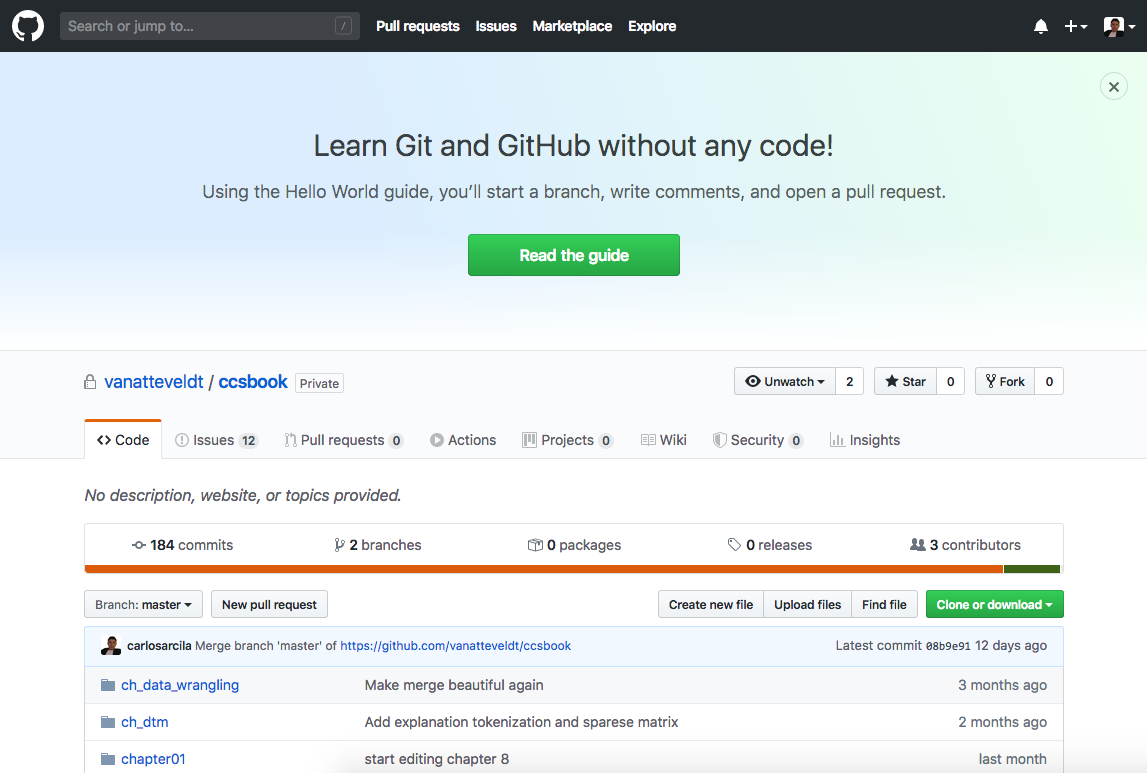
\includegraphics[width=0.9\linewidth]{figures/ch04_github}
\caption{The online repository GitHub}
\label{fig:github}
\end{figure}
 
Once you upload (or \textit{commit}) your code to GitHub you can have access to it from anywhere and will be able to track the historical changes, which in practice will allow you to have multiple versions in the very same place. You will decide if you keep the code public or private, and who to invite to edit the repository. When working collaboratively you will feel like editing a \textit{wiki} of code, while having a \textit{webpage} for your project and a \textit{net of friends} (followers), similarly to a social media. You can work locally or even from a web interface, and then synchronize the changes. When you allow colleagues to download (or \textit{clone}) your repository you are then making a good contribution to the community of developers and you can also monitor your impact. In addition to code, you can also upload other kind of files, including notebooks, and organize them in folders, just as you have it on your computer.

One extended good practice when sharing code is the use of \textit{literate programming}, which is an elegant, practical and pedagogic way to document and execute the base code. We have already mentioned in this section the importance of including documentation within your code (i.e. using the \texttt{\#} sign), but you also have the opportunity to extend this documentation (with formatted texts, images and even equations!) and put everything together to present in a logical structure all the necessary to understand the code and to run the executable lines step by step. 

There are different approaches to implement this literate programming in web and local environments, but the standard in R and Python is the use of \textit{notebooks}. In a notebook you can alternate a text processor with a executable cell to include formatted contents and blocks of code, respectively. By doing this you can include complete documentation of your scripts, and even more important you can execute each cell one step at a time (loading the results in RAM memory while the notebook is open). This last point allows you to avoid the risks of executing the whole script at once, and also to have more control of the intermediate outputs produced in your code. Once you get used to notebooks, you will probably won't want to code in a basic editor again!

The usual tool in R is the \textit{R Markdown Notebooks} and in Python the Jupyter Notebooks (see figure~\ref{fig:notebooks}), but in practice you can also deploy Python in Markdown and R in Jupyter. Both tools can help you with similar task to organize your script, though their internal technical procedures are quite different. We have chosen Jupyter to develop the examples of this book because it is a web-based interactive tool. Moreover, there several services such as Google Colab\footnote{https://colab.research.google.com}(figure~\ref{fig:colab}), that allows you remotely run these notebooks online without installing anything in your computer, making the code highly reproducible.

\begin{figure}
\centering
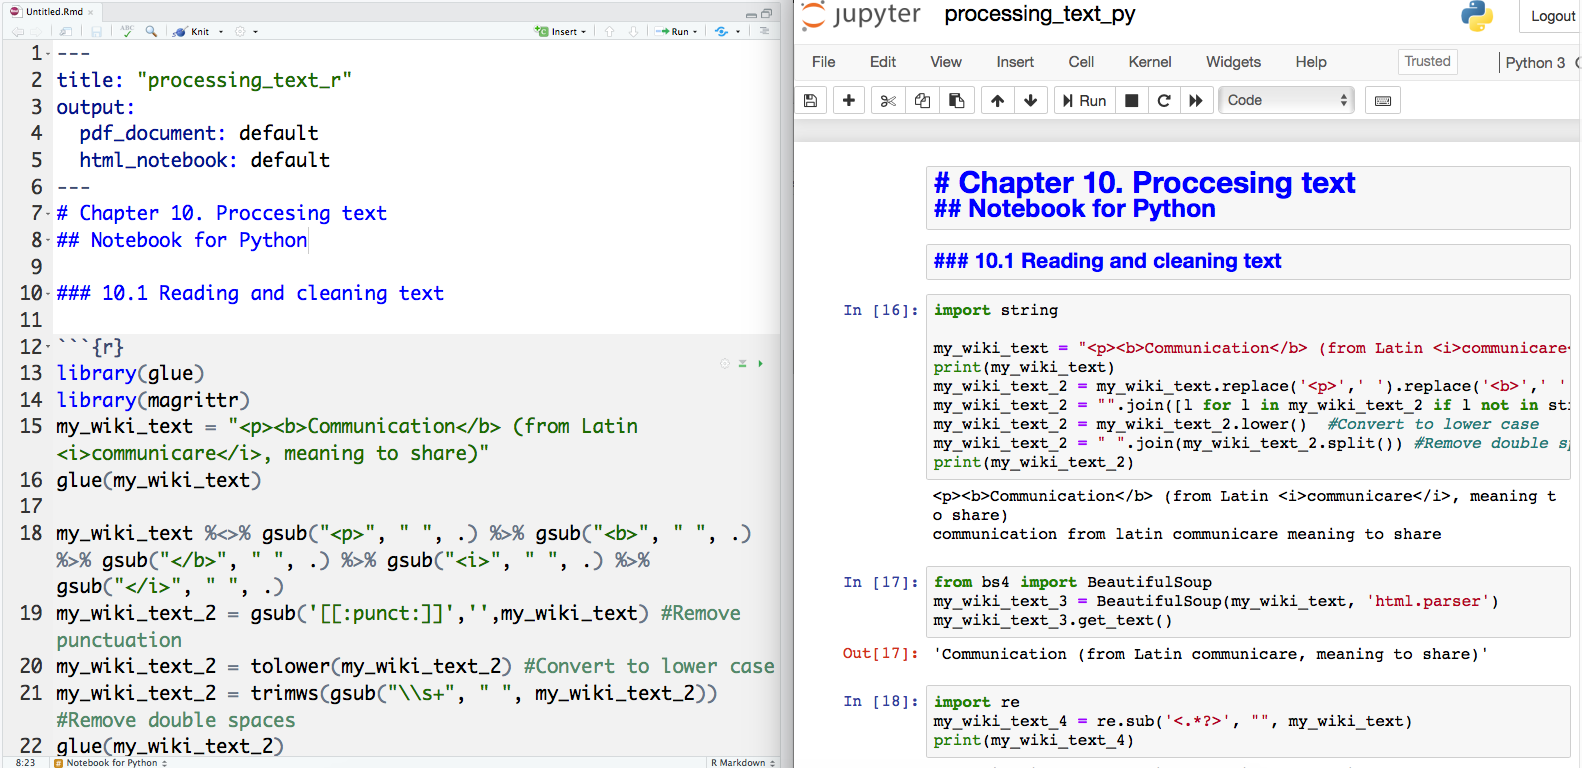
\includegraphics[width=0.9\linewidth]{figures/ch04_notebooks}
\caption{Markdown (left) and Jupyter (right) Notebooks}
\label{fig:notebooks}
\end{figure}

So far you have seen many of the possibilities that the world of code offers you from a technical and collaboration perspective. However, the practice of writing and re-using the code may also be sensitive and could lead to bad practices. The next section will deal with this ethical and normative factors.

\begin{figure}
\centering
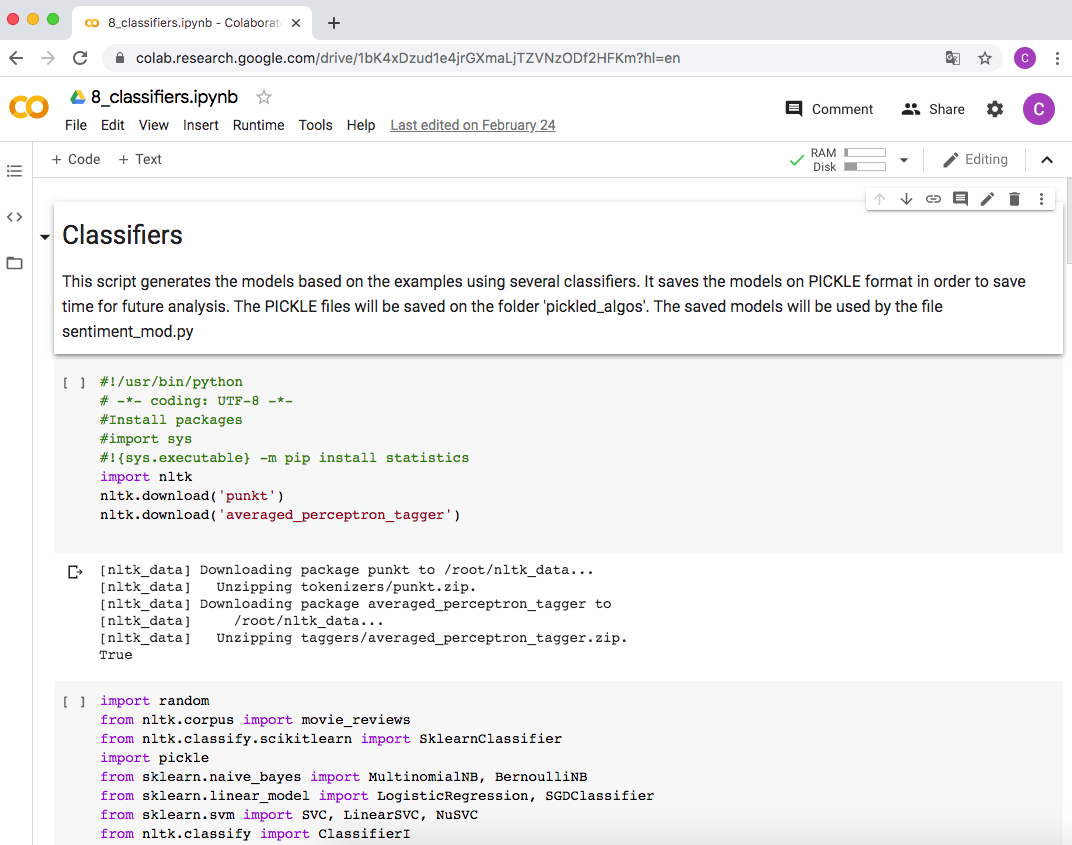
\includegraphics[width=0.9\linewidth]{figures/ch04_colab}
\caption{Jupyter notebook in Google Colab}
\label{fig:colab}
\end{figure}



\setcounter{chapter}{5}
\chapter{From file to data frame and back}
\label{chap:filetodata}


\begin{abstract}{Abstract}
  This chapter teaches you basics of file handling, such as different file formats and encodings. It introduces csv files, json files, plain text files, and binary file formats. We discuss different approaches to organizing data in files, and how to write data frames to and read them from these files].  Finally, we provide guidance for retrieving example datasets.
\end{abstract}

\keywords{file formats, encodings, reading and writing files, data frames, datasets}

\begin{objectives}
\item Know how to handle different encodings and dialects
\item Make an informed choice for a file format
\item Know how to access existing datasets
\end{objectives}

\begin{feature}
We use basic Python and R functionality to handle files. Additionally, we use \pkg{pandas} (Python) and \pkg{haven}/\pkg{tidyverse} (R) to read and write tables.
\end{feature}


\section{Why and when do we use data frames?}

In Section~\ref{sec:datatypes}, we introduced basic data types: strings (which contain text), integers (which contain whole numbers, or numbers without anything 'behind the dot'), floats (floating point numbers; numbers with decimals), and bools (Boolean values, True or False). 
We also learned that a series of multiple values (e.g., multiple integers, multiple strings) can be stored in what we call a vector (R) or a list (Python).

In most social-scientific applications, however, we do not deal with isolated series of values. We rather want to link multiple values to each other. One way to achieve this are dictionaries (see Section~\ref{sec:datatypes}).
Such data structures are really useful for nested data:
For example, if we would not want to store people's age but their addresses,
we could store a dict within a dict.
%\rpyex{chapter06/snippets/listvsdict}{CAPTION}
In fact, as we will see later in this chapter, many data that computational social scientists use come in such a format.
For instance, data about an online product can contain many reviews which in turn have various pieces of information on the review author.

But ultimately, for many social-scientific analyses, a tabular data format is preferred.
We are used to thinking of observations (cases) as rows with columns containing information or measurements about these observations (e.g., age, gender, days per week of newspaper reading, ...). It also simplifies how we can run many statistical analyses later on.

We could simply construct a list of lists to achieve such a tabular data format.
In fact, this list-of-lists technique is often used to store tabular data or matrices, and you will probably encounter it in some examples in this book or elsewhere. The list-of-lists approach is very low-level, though: If we wanted to, for instance, insert a column or a row at a specific place, writing the code to do so can be cumbersome. There are also no things like column headers, and no consistency checks: nothing would warn us if one row actually contained more 'columns' than another, which should not be the case in a rectangular table.

To make our lifes easier, we can therefore use a data structure called a data frame. 
Data frames can be generated from list-of-list structures, from dictionaries, and many others.
One way of doing so is shown in \refex{createdataframe}, but very often, you'd rather read data from a file or an online resource directly into a dataframe (see Section~\ref{sec:reading}).

\pyrex[output=both, caption=Creating a dataframe from other datastructures]{chapter06/createdataframe}

In this book, we use dataframes a lot, because they are very convenient for handling tabular data, and because they provide a lot of useful convenience functionality, instead of requiring us to re-invent the wheel all the time. In the next section, we will discuss some of them.

Of course, there are some situations when dataframes are \emph{not} a good choice to organize your data:
\begin{itemize}
\item Your data is one-dimensional. Think, for example, of resources like a list of stopwords, or a list of texts without any meta-information.
\item Your data do not have a tabular structure. Think, for example, of deeply nested data, or of very messy data.
\item Your data are so large that you cannot (or do not want to) load it into memory. For instance, if you want to process the text of all articles on Wikipedia, you probably want to process them one-by-one instead of loading all articles at the same time.
\end{itemize}

%\subsection{Basic operations on data frames}

%When retrieving data for external sources (Section~\ref{sec:gathering}), we can convert the data we retrieved into a dataframe using the techniques outlined in the previous paragraphs. In many other cases, we will read them directly from files instead (Section~\ref{sec:reading}).

Therefore, you will come across (and we will introduce you to) examples in which we do \emph{not} use data frames to organize our data.
But in most cases we will, because they make our life easier:
Once we constructed our data frame, we have a range of handy functions at our disposal, that allow us to select rows or columns, add new rows or columns, apply functions to them, and so on.
We will discuss these in Chapter~\ref{chap:datawrangling}.

But how do we -- toy examples like those in \refex{createdataframe} aside -- get data into and out of dataframes? 




%Table~\ref{tab:dataframecommands} gives an overview of some of them. Many of these commands will come back in subsequent chapters, but we encourage you to already play around a bit with them. That is more fun with a real dataset - and that's why we will load some in the next section.


%\begin{table}[]
%\caption{Basics of data frame handling}
%\label{tab:dataframecommands}
%\begin{tabularx}{\textwidth}{XXXXX}
%\toprule
%                         & pandas data frame                 & R data.frame & R tibble \\ \midrule
%select rows by index     & df.iloc{[}1, ...... ..            &              &          \\
%select columns by number & df.iloc...                        &              &          \\
%select columns by name   & df{[}'mycolumn'{]} or df.mycolumn &              &          \\ \bottomrule
%\end{tabularx}
%\end{table}




\section{Reading and saving data}
\label{sec:reading}

\subsection{The role of files}

In statistical software like SPSS or Stata, or in all typical office applications for that matter, you \emph{open} a file, do some work on it, and then \emph{save} the changes to the same file once you are done. You basically ``work on that file''.

That's not how your typical workflow in R or Python looks like. Here, you work on one or multiple data frames (or some other data structures). That means that you might start by \emph{reading} the contents of some file into a data frame, but once that is done, there is no link between the dataframe and that file any more. Once your work is done, you can save your dataframe to a file, of course, but it is a good practice not to overwrite your input file, so that you can always go back to where you started. A typical workflow would rather look like this:
\begin{enumerate}
\item Read raw data from file \ttt{myrawdata.csv} into data frame \ttt{df}"
\item Do some operations and analyses on df
\item Save df to file \ttt{myfinaldata.csv}
\end{enumerate}
Note that the last step is not even necessary, but may be handy if running the script takes very long, or if you want to re-distribute the resulting file.

The format in which we read files into a data frame and the format to which we save our final data frame also by no means needs to be identical. We can, for example, read data created by someone else in Stata's proprietary \ttt{.dta} format into a dataframe and later save it to a .csv table.

While we sometimes do not have the choice in which format we get our input data, we have a range of options regarding our output data. We usually prefer formats that are \emph{open} and \emph{interoperable} for this, which ensures that they can be used by as many people as possible, also in the future, and that they are not tied to any specific (proprietary) product.

The most common file formats that are relevant to us are listed in Table~\ref{tab:fileformats}. \ttt{txt} files are particularly useful for long texts (think of one file containing one newspaper article or even a whole book), but they are bad for storing associated meta data. \ttt{csv} files are the default choice for tabular data, and \ttt{json} files allow us to store nested data in a dictionary-like format. 

For the sake of completeness, we also listed the native Python and R formats pickle, RDS, and RDA. Because their lack of interoperability, they are not very suitable for long-term storage or for sharing data, but they can have a place in a workflow as an intermediate step to solve the issue that none of the other formats are able of storing all properties of a dataframe (e.g., the csv file cannot store whether a given column in an R dataframe is to be understood as containing strings such as 'man', 'woman', 'non-binary' or a factor with the three levels man, woman, non-binary). If it is of importance to store an object (such as a dataframe) exactly as-it-is, we can use these formats. One of the rare instances where we use these formats is in \refex{reuse}, where we store machine learning models for later reuse.

\begin{table}[]
\caption{Basics of data frame handling \label{tab:fileformats}}{%
\begin{tabular}{@{}llll@{}}
\toprule
        & Used for?             & open   & interoperable?\\ \midrule
txt     & plain text            &yes & yes            \\
csv     & tabular data          & yes & yes            \\
json    & nested data, key-value pairs   & yes & yes             \\ 
pickle  & Python objects        & yes & no     \\ 
RDS/RDA & R objects             & yes & no \\ \bottomrule
\end{tabular}}{}
\end{table}


\subsection{Encodings and dialects}
\label{sec:encodings}
Plan \ttt{txt} files, \ttt{csv} files, and \ttt{json} files are all files that are based on text. Unlike binary file formats, you can read them in any text editor. Try it yourself to understand what is going on under the hood. 

Download a csv file (such as \url{http://cssbook.net/d/gun-polls.csv})
and open it in a text editor of your choice. Some people swear that their preferred editor is the best (google to learn about the vi vs. emacs war for some entertainment), but if you have no strong feeling, then Notepad++, Atom, or Sublime may be good choices that you may want to look into.

As you will see (Figure~\ref{fig:csv-in-editor}), a csv file internally just looks like a bunch of text in which each line represents a row and in which the columns are separated by a comma (hence the name comma seperated values (csv)).
Looking at the data in a text editor is a very good way to find out what happens if reading your files into a data frame does not work as expected - which can happen more frequently than you would expect.

Mostly due to historical reasons, not every text based file (which, as we have seen, includes csv files) is internally stored in the same way.
For a long time, it was common to \emph{encode} in such a way that one character mapped to one byte. That was easy from a programming perspective (after all, the n-th character of a text can directly be read from and written to the n-th byte of a file) and also storage-efficient. But given that a byte consists of 8 bits, that means that there are only 256 possible characters. All letters in the alphabet in uppercase, again in lowercase, numbers, punctuation, some control characters -- and you are out of characters. Due to this limitation, there were different encodings or codepages for different languages that told a program which value should be interpreted as which character.

We all know the phenomenon of garbled special characters, like German umlauts or Scandinavian characters like ø, å, or œ being displayed as something completely different. This happens when files are read with a different encoding than the encoding that was used for creating them.

In principle, this issue has been solved due to the advent of Unicode. Unicode allows to handle all characters from all scripts, including emoticons, Korean and Chinese characters, and so on. The most popular encoding for Unicode characters is called UTF-8, and it has been around for decades. 

To avoid any data loss, it is advisable to make sure that your whole workflow uses UTF-8 files. By far most modern applications support UTF-8, even though some still by default use a different encoding (e.g., 'Windows-1252') to store data. As Figure~\ref{fig:csv-in-editor} illustrates, you can use a text editor to find out what encoding your data has, and many editors also offer an option to change the encoding. However, you cannot recover what has been lost (e.g., if at one point you saved your data with an encoding that only allows 256 different characters, it follows logically that you cannot recover that information).


\begin{figure}
\centering
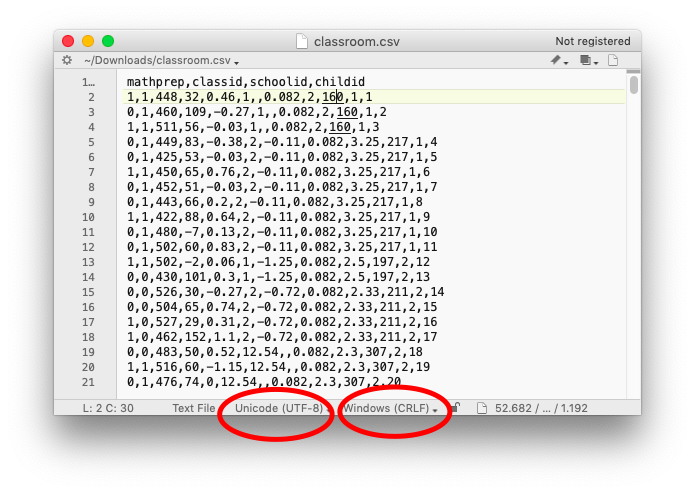
\includegraphics[width=0.9\linewidth]{figures/ch6_csv-in-editor}
\caption{A csv file opened in a text editor, illustrating that the columns are separated by commas, and showing the encoding and the line endings.}
\label{fig:csv-in-editor}
\end{figure}

As we will show in the practical code examples below, you can also force Python and R to use a specific encoding, which can come in handy if your data arrives in a legacy encoding.

Related to the different encodings a file can have, but less problematical, are different conventions of how a \emph{line ending} is denoted. Windows-based programs have been using a Carriage Return followed by a Line Feed (denoted as \texttt{\textbackslash r\textbackslash n}), very old versions of MacOS used a Carriage Return only (\texttt{\textbackslash r}), and newer versions of MacOS as well as Linux use a Line Feed only (\texttt{\textbackslash n}). In our field, the Linux (or Unix) style line endings have become most dominant, and Python 3 even automatically converts Windows style line endings to Unix style line endings when reading a file -- even on Windows itself.

A third difference is the use of so-called \emph{byte-order markers} (BOM). In essence, a BOM is an additional byte added to the beginning of a text file to indicate that it is a UTF-encoded file and to indicate in which order the bytes are to be read (the so-called endianness). While informative, this can cause trouble if your program does not expect that byte to be there. In that case, you might either want to remove it or explicitly specify the encoding as such (e.g., 'utf-8-bom' instead of 'utf-8' in the examples below).


In short, the most standard form in which you probably want to encode your data is in UTF-8 with Linux-style line endings without the use of a byte-order marker.


In the case of reading and writing csv files, we thus need to know the encoding, and potentially also the line ending conventions and the presence of a byte-order marker. However, there are also some additional variations that we need to consider. There is no single definition of how a csv file needs to look like, and there are multiple dialects that are widely used. They mainly differ in two aspects: the delimiter that is chosen, and the quoting an/or escaping of values.

First, even though csv stands for comma separated values, one could use other characters instead of a comma to separate the columns. In fact, because many countries use a comma instead of a dot to as a decimal separator (\$10.30 vs 10,30€), in these countries a semicolon (';') is used instead of a comma as  column delimiter. To avoid the possible confusion, others use a tab character (\texttt{\textbackslash t}) to seperate columns. Sometimes, these files are then called a tab-seperated file, and instead of .csv, they may have a file extension such as \ttt{.tsv}, \ttt{.tab}, or even \ttt{.txt}. However, this does not change the way how you can read them - but what you need to know is whether your columns are seperated by \texttt{,}, \texttt{;}, or \texttt{\textbackslash t}. 

Second, there may be different ways of how to deal with strings as values in a csv file. For instance, it may be that a specific value contains the same character that is also used as a delimiter. These cases are usually resolved by either putting all strings into quotes, putting only strings that contain such ambiguities in quotes, or by prepending the ambigous character with a specific escape character. Most likely, all of this is just handled automatically under the hood, but in case of problems, you might want to look into this and check out the documentation of the packages you are using on how to specify which strategy is to be used.

Let's get practical and try out reading and writing files into a data frame (\refex{readfiles}).

\pyrex[output=none, caption=Reading files into a dataframe]{chapter06/readfiles}

Of course, we can read more than just csv files. In the Python
example, you can use tabcompletion to get an overview of all file
formats Python supports: Type |pd.read| and then press the TAB key to
get a list of all supported files. For instance, you could to
|pd.read_excel('test.xlsx')|, |df3 = pd.read_stata('test.dta')|, or
|df4 = pd.read_json('test.json')| Similarily, for R, you can hit TAB
after typing |haven::| to get an overview over functions such as
|read_spss|.

\subsection{File handling beyond data frames}
Dataframes are a very useful data structure for organizing and analyzing data, and will come back in many examples in this book.
However, not all things that we might want to read from a file needs to go into a dataframe.
Imagine if we have a list of words that we later want to remove from some texts (so-called stopwords, see \refchap{protext}).
We could make a list (or vector) of such words directly in our code. 
But if we have more than a couple of such words, it is easier and more readable to keep them in an external file. We could create a file \texttt{stopwords.txt} in a text editor with one of such words per line:

\begin{lstlisting}
and
or
a
an
\end{lstlisting}

If you are too lazy to create this list yourself, you could also
download one from \url{http://cssbook.net/d/stopwords.txt} and save it
in the same directory as your Python or R script.

Then, you can read this file into a vector or list  (see \refex{readingstopwords}).

\pyrex[output=none, caption=Reading files without dataframes]{chapter06/stopwords}

\pyrex[output=none, caption={More examples for reading from and writing to files. Because dictionaries do not exist in R and handling non-rectangular data is more uncommon in R, we do not show an example for direct interaction with JSON files without involvement of a dataframe in the R example.}]{chapter06/extendedfilehandling}

\refex{extendedfilehandling} provides you with some more elaborate code examples that allows us to dig a bit deeper into the general way of handling files.

In the Python example,  we can open a file and assign a handle to it that allows us to refer to it (the name of the handle is arbitrary, let's just call it \texttt{f} here.
Then, we can use a for loop to iterate over all lines in the file and add it to a list

The \texttt{mode = 'r'} specifies that we want to read from the file. \texttt{mode = 'w'} would open the file for writing, create it if necessary, and immediately deletes all content that may have been in there if the file already existed (!).
Note that the \texttt{.strip()} is necessary to remove the line ending itself, and also possible whitespace at the beginning or end of a line.
If we want to save our stopwords, we can do this in a similar way: We first open the file (this time, for writing), and then use the file handle's methods to write to it.
We are not limited to plain text files, here. For instance, we can use the same approach to read json files into a python dict or to store a python dict into a json file.

We could also combine this with a for loop that goes over all files in a dictionary.
Imagine we have a folder full of positive movie reviews, and another one full of negative movie reviews that we want to use to train a machine learning classifier (see Section~\ref{sec:supervised}).
Let's further assume that all these reviews are saved as \texttt{.txt} files.
We can iterate over all of them, as shown in \refex{reviewdata}. If you want to read text files into a dataframe in R, the \pkg{readtext} package may be interesting for you.


\section{Data from online sources}
\label{sec:gathering}

Many data that are interesting to those analyzing communication are
nowadays gathered online.  In Chapter~\ref{chap:scraping}, you will
learn how to use APIs to retrieve data from web services, and how to
write your own web scraper to automatically download large quanties of
web pages and extract relevant information. For instance, you might
want to retrieve customer reviews from a website or articles from news
sites.

In this section, however, we will focus on how to re-use existing
datasets that others have made available online. For instance, the
open science movement has led to more and more datasets being shared
openly using repositories such as Dataverse, Figshare, or
others. Re-using existing data can be very good for several reasons:
First, to confirm (or not) the conclusions drawn by others; second, to
not waste resources by re-collecting very similar or even identical
data all over again; and third, because gathering a large,
high-quality dataset might just not be feasible with your means. This
is especially true when you need annotated (i.e., hand-coded) data for
supervised machine learning purposes (Chapter~\ref{chap:introsml}).

We can distinguish between two types of existing online datasets:
datasets that are inherently interesting, and so-called toy datasets.

Toy datasets may include made-up data, but often, these data are
real. However, they are not analyzed to gain scientific insights (any
more), as they may be too small, outdated, or already analyzed
all-over again. These provide a great way, though, to learn and
explore new techniques: After all, the results and the characteristics
of the data are already known. Hence, such toy datasets are often
even included in R and Python packages. Some of them are really
well-known in teaching (e.g., the iris dataset containing measurements
of some flowers; or the titanic dataset containing statistics on
survival rates of passengers on the Titanic; or the MPG dataset on car fuel consumption). Many of these are included
in packages like \pkg{scikit-learn}, \pkg{seaborn}, or \pkg{ggplot2}-- have a look at their documentation.

For instance, the 20 Newsgroups dataset contains $18,846$ posts from
newsgroups plus the groups where they were posted
(\refex{20newsgroups}). This can be an interesting resource for
exercising with natural language processing, unsupervised, and
supervised machine learning. Another interesting resource are
collections of political speeches, such as the state-of-the-union
speeches from the US, which are available in multiple packages
(\refex{sotudata}).
Other interesting datasets with large collections of textual data may
be the Financial News dataset compiled by \cite{Chen2017} or the
political news dataset compiled by \cite{Horne2018}.


\pyrex[output=py, input=both,caption={In Python, \pkg{scikit-learn} has a convenience function to automatically download the 20 newsgroup dataset and automatically clean it up. In R, you can download the raw version (there are multiple copies floating around on the internet) and perform the cleaning yourself.}]{chapter06/20newsgroups}

\pyrex[output=r, input=both, format=table, caption={A collection of US state-of-the-union speeches is available in multiple packages in various forms.}]{chapter06/sotudata}



There are also some more generic ressources that you may want to consider for finding
more datasets to play around with. On  \url{https://datasetsearch.research.google.com},
you can search for datasets of all kinds, both really interesting ones and toy datasets.
Another great research is \url{https://kaggle.com}, a site that hosts data
science competitions.






% \part{From Data to Science}

\setcounter{chapter}{6}
\chapter{Data Wrangling}
\label{chap:datawrangling}

\begin{abstract}{Abstract}
This chapter shows you how to do `data wrangling' in R and Python.
Data wrangling is the process of transforming raw data into a shape that is suitable for analysis. The sections of this chapter first take you through the normal data wrangling pipeline of
filtering, changing, grouping, and joining data. Finally, the last section shows how you can
reshape data.
\end{abstract}

\keywords{Data wrangling, data cleaning, filtering, merging, reshaping}

\begin{objectives}
\item Filter rows and columns in data frames
\item Compute new columns and summary statistics for data frames
\item Reshape and merge data frames
\end{objectives}

\begin{feature}
  This chapter uses functions from the package \pkg{tidyverse} (including: \pkg{ggplot2}, \pkg{dplyr}, \pkg{tidyr}, \pkg{pusss}, \pkg{tibble}, \pkg{stringr} and \pkg{forcats}) in R and the package \pkg{pandas} in Python. In this chapter we read the data directly from the Internet page of this book, but instead of a URL you can also use a local file name.
\end{feature}


\section{Filtering, selecting and renaming}


\paragraph{Selecting and renaming columns}
A first clean up step we often want to do is removing unnecessary columns and renaming columns with unclear or overly long names.
In particular, it is often convenient to rename columns that contain spaces or non-standard characters, so it is easier to refer to them later.

\paragraph{Selecting rows}
As a next step, we can decide to filter out certain rows.
For example, we might want to use only a subset of the data,
or we might want to remove certain rows because they are incomplete or incorrect.

As an example, FiveThirtyEight published a quiz about American public opinon about guns,
and were nice enough to also publish the underlying data\footnote{https://projects.fivethirtyeight.com/guns-parkland-polling-quiz/; see https://github.com/fivethirtyeight/data/tree/master/poll-quiz-guns for the underlying data}.
\refex{data-filter} gives an example of loadnig and cleaning this data set, starting with the \verb+read_csv+ function to load the data directly from the Internet.
This data set contains one poll result per row, with a Question column indicating which question was asked,
and the columns listing how many Americans (adults or registered voters) were in favor of that measure, in total and for Republicans and Democracts.
Next, the columns \emph{Republican} and \emph{Democratic Support} are renamed to shorten the names and remove the space.
Then, the URL column is dropped using the \verb+select+ (R) or \verb+drop+ (python) function.
Notice that the result of these operations is assigned to the same object \verb+d+.
This means that the original \verb+d+ is overwritten.

\note{[R] In R, the \texttt{select} function is quite versatile.
  You can specify multiple columns using \texttt{select(d, column1, column2)} 
  or by specifying a range of columns: \texttt{select(d, column1:column3)}.
  Both commands keep only the specified columns. 
  As in the example, you can also specify a negative selection with the minus sign: 
  \texttt{select(d, -column1)} drops \texttt{column1}, keeping all other columns.
  Finally, you can rename columns in the select command as well: 
  \texttt{select(d, column1=col1, column2)} renames \texttt{col} to \texttt{column1},
  keeps that column and \texttt{column2},and drops all other columns.
  }
  
In line 6, we filter the data set to list only the polls on whether teachers should be armed
(you can understand this is close to our heart).
This is done by comparing the value of the Question column to the value \verb+'arm-teachers'+.
This comparison is done with a double equals sign (\verb+==+).
In both python and R, a single equals sign is used for assignment,
and a double equal sign is used for comparison.
A final thing to notice is that while in R we used a function (\verb+filter+) to filter out rows,
in python we \emph{index} the data frame using square brackets on the \verb+loc+(ation) attribute: \verb+d.loc[]+.

Note that we chose to assign the result of this filtering to \verb+d2+,
so after this operation we have the original full data set \verb+d+ as well as the subset \verb+d2+ at our disposal.
In general, it is your choice whether you overwrite the data by assigning to the same object,
or create a copy by assigning to a new name.
If you will later need to work with a different subset, it is smart to keep the original so you can subset it again later.
On the other hand, if all your analyses will be on the subset, you might as well overwrite the original.
We can always re-download it from the internet (or reload it from our harddisk) if it turns out we needed the original anyway. 

\pyrex[caption=Filter,output=r,format=html]{ch_data_wrangling/data-filter}



\section{Calculating values}
\label{sec:calculate}

Very often, we need to calculate values for new columns or change the content of existing columns.
For example, we might wish to calculate the difference between two columns,
or we may need to clean a column by correcting clerical errors or converting between data types.

In these steps, the general pattern is that a column is assigned a new value based on
a calculation that generally involves other columns.
In both R and Python, there are two general ways to accomplish this.
First, you can simply assign to an existing or new column,
using the column selection notation discussed in \refsec{datatypes}:
\verb+df["column"] = ...+ in Python, or \verb+df$column = ...+ in R.

Both Python and R also offer a function that allows multiple columns to be changed,
returning a new copy of the data frame rather than changing the original data frame.
In R, this is done using the \verb+mutate+ function, which is the recommended way to compute values.
The Python equivalent, \verb+assign+, is used more rarely as it does not offer many advantages over direct assignment.

In either case, you can use arithmetic: e.g. \verb|rep - dem| for computes the difference between these columns.
This works directly in R \verb+mutate+,
but in Python or in R direct assignment you also need to specify the name of the dataframe.
In python, this would be \verb+d.rep - d.dem+, while in R this is \verb+d$rep - d$dem+. 

In many cases, however, you want to use various functions to perform tasks like cleaning and data conversion
(see \refsec{function} for more explanation of built-in and custom functions).
For example, to convert a column to numeric you would use the \verb+as.numeric+ (R) or \verb+pd.to_numeric+ (Python) function.
Both functions take a column as argument and convert it to a numeric column.

Almost all R functions work on whole columns like that.
In Python, however, many functions work on individual values rather than columns.
To apply a function on each element of a column, you can use \verb+df.col.apply(my_function)+
(where df and col are the names of your dataframe and column). 
There are more built-in functions that you can call on a column, for example \verb+df.col.fillna+ replaces
missing values, and \verb+df.col.str.replace+ does a find and replace.
Note that these functions (like most functions in pandas) work on whole columns,
so there is no need to \verb+apply+ them. 

%TODO should we give or point to some overview of possible functions?

\pyrex[output=r,format=html,caption=Mutate]{ch_data_wrangling/mutate}

To illustrate these possibilities, \refex{mutate} has code for cleaning a version of the Guns Polls
in which we intentionally introduced two problems: we added some typos to the `rep' column
and introduced a missing value in the `Support' column.
To clean this, we perform three steps: First, we remove all non-numeric characters using a regular expression
(see \refsec{regex} for more information on text handling and regular expressions).
Next, we need to explicitly convert the resulting column into a numeric column so we can later use it in calculations.
Finally, we replace the missing value by the column mean
(of course, it is doubtful that that is the best strategy for imputing missing values here,
we do it mainly to show how one can deal with missing values technically).

The cleaning process is actually performed twice: lines 5-10 use direct assignment,
while lines 12-18 use the \verb+mutate+/\verb+assign+ function.
Finally, lines 20-26 show how you can define and apply a custom function to combine the first two cleaning steps.
This can be quite useful if you use the same cleaning steps in multiple places,
since it reduces the repetition of code and hence the possibility of introducing bugs or inconsistencies. 

Note that all these versions work fine and produces the same result.
In the end, it is up to the researcher to determine which feels most natural in the circumstances.
As noted above, in R we would generally prefer \verb+mutate+ over direct assignment,
mostly because it fits nicely into the tidyverse workflow and you do not need to repeat the data frame name.
In Python, we would generally prefer the direct assignment, unless it is desired to make a copy of the data
with the changes made, in which case \verb+assign+ can be more useful. 




\section{Grouping and aggregating}

The functions we used to change data above operated on individual rows.
Sometimes, however, we wish to compute summary statistics of groups of rows.
This essentially shifts the unit of analysis to a higher level of abstraction.
For example, we could compute per-school statistics from a data file containing information per student;
or we could compute the average number of mentions of a politician per day from a file containing information per articles.

In data analysis, this is called \emph{aggregation}.
In both Python and R, it consists of two steps:
First, you define which rows are \emph{grouped} together to form a new unit
by specifying which column identifies these groups.
In the previous examples, this would be the school name or ID or the date of each article.
It is also possible to group by multiple columns, for example to compute the average per day per news source.

The next step is to specify one or more summary (or \emph{aggregate}) functions to be computed over the desired value columns.
These functions compute a summary value, like the mean, sum, or standard deviation, over all the values belonging to each group.
In the example, to compute average test scores per school we would apply the average (or mean) function to the test score value column.
In general, you can use multiple functions (e.g.  mean and variance) and multiple columns (e.g. mean test score and mean parental income).

The resulting dataset is reduced both in rows and in columns.
Each row now represents a group of previuos cases (e.g. school or date),
and the columns are now only the grouping columns and the computed summary scores.

\refex{data-aggregate} shows the code in R and Python to define groups and compute summary values.
First, we group by poll \emph{question}; and for each question, we compute the average and standard deviation.
The syntax is a little different for R and Python, but the idea is the same:
first we create a new variable \verb+groups+ that stores the grouping information,
and then we create the aggregate statistics.
In this example, we do not store the result of the computation, but print it on the screen.
To store the results, simply assign it to a new object as normal.

\pyrex[caption=Aggregation,output=r,format=table]{ch_data_wrangling/aggregate}

In R, you use the \pkg{dplyr} function \fn{group\_by}  to define the groups,
and then call the function \fn{summarize~} to compute summary values by specifying
\verb+name=function(value)+.

In Python, the grouping step is quite similar.
In the summarization step, however, you specify which summaries to compute in a dictionary%
\footnote{See \refsec{datatypes} for more information on working with dictionaries}.
The keys of the dictionary lists the value columns to compute summaries of,
and the values contain the summary functions to apply, so \verb+{'value': [function]}+.

\subsection{Combining multiple operations}

In the examples above, each line of code (often called a \emph{statement}) contained a single operation, generally a function call.
The general shape of each line in R was \verb+data = function(data, arguments)+, that is, the data is provided as the first argument to the function.
In Python, you specify the object on which to call the function with a period,
i.e. \verb+object.function(arguments)+.

Although there is nothing wrong with limiting each line to a single operation, both languages allow multiple operations to be chained together.
Especially for grouping and summarizing, it can make sense to link these operations together as they can be thought of as a single `data wrangling' step.

In Python, this can be achieved by adding the second \verb+.function()+ directly to the end of the first statement.
Essentially, this calls the second function on the result of the first function: \verb+data = data.function1(arguments).function2(arguments)+.

In R, the data is of course included in the function arguments, so an alternative method is needed to chain function calls.
This is done using the \emph{pipe operator} (\verb+%>%+) from the (cutely named) \pkg{magrittr} package.
The pipe operator inserts the result of the first function as the first argument of the second function.
More technically, \verb+f1(d) %>% f2()+ is equivalent to \verb+f2(f1(d))+.
This can be used to chain multiple commands together, e.g. \verb+data = data %>% function1(arguments) %>% function2(arguments)+.

\pyrex[caption=Combining multiple functions,output=r,format=table]{ch_data_wrangling/aggregate2}{

\refex{data-aggregate2} shows the same operation as above, but chained into a single statement.


\subsection{Adding summary values}

Rather than reducing a data frame to contain only the group-level information,
it is sometimes desirable to add the summary values to the original data.
For example, if we add the average score per school to the student-level data,
we can then determine whether individual students outperform the school average.

Of course, the summary scores are the same for all rows in the same group:
all students in the same school have the same school average.
So, these values will be repeated for these rows, essentially
mixing individual and group level variables in the same data frame.

\pyrex[caption=Adding summary values to individual cases,output=r,format=table]{ch_data_wrangling/transform}

\refex{data-transform} shows how this can be achieved in Python and R,
computing the mean support per question and then calculating how each poll deviates from this mean. 

In R, the code is very similar to \refex{data-aggregate2} above, simply
replacing the \pkg{dplyr} function \fn{summary} by the function \fn{mutate} discussed above.
In this function you can mix summary functions and regular functions, as shown in the example:
first the mean per group is calculated, followed by the deviation of this mean.

The Python code also uses the same syntax used for computing new columns.
The first line selects the \emph{Support} column on the grouped dataset,
and then calls the \pkg{pandas} function \fn{transform} on that column to compute the mean per group,
adding it as a new column by assigning it to the column name.
The second line uses the regular assignment syntax to create the deviation based on the support and calculated mean. 

\section{Merging data}

In many cases, we need to combine data from different sources or data files.
For example, we might have election poll results in one file and socio-economic data per area in another.
To test whether we can explain variance in poll results from factors such as education level,
we would need to combine the poll results with the economic data.
This process is often called merging or joining data.

\subsection{Equal units of analysis}

%\pyrex[caption=Private and Pulic Capital data (source: Piketty 2014)]{ch_data_wrangling/piketty}

\begin{ccsexample}
  \doublecodex{ch_data_wrangling/piketty_1}
  \codexoutputtable{ch_data_wrangling/piketty_1.r}
  \doublecodex{ch_data_wrangling/piketty_2}
  \codexoutputtable{ch_data_wrangling/piketty_2.r}
\caption{Private and Pulic Capital data (source: Piketty 2014)}\label{ex:piketty}
\end{ccsexample}


The easiest joins are when both data sets have the same unit of analysis,
i.e. the rows represent the same units.
For example, consider the data on public and private capital ownership published by
\cite{piketty} alongside his landmark book \emph{Capital in the 21st Century}.
As shown in \refex{piketty}, he released separate files for public and private capital ownership.
If we would want to analyse the relationship between these (for example to recreate Figure 3.6 on page 128 of that book),
we first need to combine them into a single data frame.

To combine these data frames, we use the \pkg{pandas} function \fn{merge} in Python or the \pkg{dplyr} method \fn{full\_join} in R.
Both methods join the data frames on one or more \emph{key} columns.
The key column(s) identify the units in both data frames, so in this case the \emph{Year} column.
Often, the key column is some sort of identifier, like a respondent or location ID.
The resulting data frame will contain the shared key column(s), and all other columns from both joined data frames.

In both Python and R, all columns that occur in both data frames are by default assumed to be the key columns.
In many cases, this is the desired behaviour as both data frame may contain e.g. a \emph{Year} or \emph{RepondentID} column.
Sometimes, however, this is not the case.
Possibly, the key column is called differently in both data frames, e.g. \emph{respID} in one and \emph{Respondent} in the other. 
It is also possible that the two frames contain columns with the same name,
but which contain actual data that should not be used as key.
For example, in the Piketty data shown above the key column is called \emph{Year} in both frames,
but they also share the columns for the countries which are data columns.

In these cases, it is possible to explicitly specify which columns to join on (using the \verb+on=+ (Python) / \verb+by=+ argument).
However, we would generally recommend preprocessing the data first and select and/or rename columns such that the only shared columns are the key columns.
The reason for that is that if columns in different data frames mean the same thing (i.e. \emph{respID} and \emph{Respondent}), they should generally have the same name to avoid confusion.
In the case of `accidentally' shared column names, such as the country names in the current example,
if is also better to rename them so it is obvious which is which in the resulting data set:
if shared columns are not used in the join, by default they get `.x' and `.y' appended to their name, which is not very meaningful.
Even if the key column is the only shared column, however, it can still be good to explicitly select that column to make it clear to the reader (or the future you) what is happening. 

\begin{ccsexample}
\doublecodex{ch_data_wrangling/capital_1}
\codexoutputtable{ch_data_wrangling/capital_1.r}
\doublecodex{ch_data_wrangling/capital_2}
\doubleoutput{ch_data_wrangling/capital_2}
\caption{Merging private and public data for France}\label{ex:merge}
\end{ccsexample}


%\pyrex[caption=Merging private and public data for France]{ch_data_wrangling/capital}

This is shown in \refex{merge}.
The first two lines select only the \emph{Year} and \emph{France} columns, and rename the \emph{France} column to indicate whether it is the private or public data.
Lines 3 and 5 do the actual join, with and without the explicit selection of key column, respectively.
This is then used to compute the correlation between private and public capital, 
which shows that there is a weak but (just) significant negative correlation ($\rho=-.32, p=.04$)%
\footnote{Of course, the fact that this is time series data means that the independence assumption of regular correlation is violated badly, so this should be interpreted as a descriptive statistic, e.g. in the years with high private capital there is low public capital and the other way around}.

\subsection{Inner and Outer joins}

In the example above, both data sets had exactly one entry for each unit (year), making it the most straightforward case.
If either (or both) of the data sets are missing units, however, you need to specify how to deal with this.

\reftab{joins} list the 4 possible ways of joining, keeping all rows (\emph{outer join}), only rows present in both (\emph{inner join}), or all rows from one of the sets and matching rows from the other (\emph{left} or \emph{right join}).
In all cases except inner joins, this can create units where information from one of the data sets is missing.
This will be lead to missing values (|NA|/|NaN|) being inserted in the columns of the data sets with missing units.

\SaveVerb{py_full}|d1.merge(d2, how='outer')|
\SaveVerb{py_inner}|d1.merge(d2, how='inner')|
\SaveVerb{py_left}|d1.merge(d2, how='left')|
\SaveVerb{py_right}|d1.merge(d2, how='right')|
\SaveVerb{r_full}|full_join(d1,d2)|
\SaveVerb{r_inner}|inner_join(d1,d2)|
\SaveVerb{r_left}|left_join(d1,d2)|
\SaveVerb{r_right}|right_join(d1,d2)|


\begin{table}
  \caption{Different types of joins between datasets d1 and d2\label{tab:joins}}{%
  \begin{tabularx}{\linewidth}{lXll}
    \toprule
    Type &  Description  & R & Python \\
    \midrule
    Outer &  All units from both sets & \UseVerb{r_full} & \UseVerb{py_full} \\
    Inner & Only units that are in both sets & \UseVerb{r_inner} & \UseVerb{py_inner} \\
    Left & All units from left-hand set & \UseVerb{r_left} & \UseVerb{py_left} \\
    Right & All units from right-hand set & \UseVerb{r_right} & \UseVerb{py_right} \\  
    \bottomrule
  \end{tabularx}}{}
\end{table}


In most cases, you will either use inner join or left join.
Inner join is useful when information should be complete,
or where you are only interested in units with information in both data sets.
In general, when joining sets with the same units, it is smart to check the number of rows before and after the operation.
If it decreases, this shows that there are units where information is missing in either set.
If it increases, it shows that apparently the sets are not at the same level of analysis,
or there are duplicate units in the data.
In either case, an unexpected change in the number of rows is a good indicator that something is wrong.

Left joins are useful when you are adding extra information to a `primary' data set.
For example, you might have your main survey results in a data set,
to which you want to add metadata or extra information about your respondents.
If this data is not available for all respondents, you can use a left join to add the information
where it is available, and simply leave the other respondents with missing values.

A similar use case is if you have a list of news items, and a separate list of items that were coded
or found with some search term. Using a left join you keep all news items, and add the coding where it is available.
Especially if items that had zero hits of a search term are excluded from the search results,
you might use a left join followed by a calculation to replace missing values by zeroes to indicate that the counts for
items aren't actaully missing, but were zero. 

Of course, you could also use a right join to achieve the same effect.
It is more natural, however, to work from your primary data set and add the secondary data,
so you will generally use left joins rather than right joins.

Outer (or full) joins can be useful when you are adding information from e.g. multiple survey waves,
and you want to include any respondent that answered any of the waves.
Of course, you will have to carefully think about how to deal with the resulting missing values in the substantive analysis. 

\subsection{Nested data}

The sections above discuss merging two data sets at the same level of analysis,
i.e. with rows representing the same units (repondents, items, years) in both sets.
It is also possible, however, to join a more aggregate (high level) set with a more detailed data set.

For example, you might have respondents that are part of a school or organizational unit.
It can be desirable to join the respondent level information with the school level information,
for example to then explore differences between schools or do multilevel modelling.

For this use the same commands as for equal joins.
In the resulting merged data set, information from the group level will be duplicated for all individuals in that group.

For example, take the two data sets shown in \refex{primary}.
The \texttt{results} data set shows how many votes each US 2016 presidential primary candidate received in each county:
Bernie Sanders got 544 votes in Autauga County in the US state of Alabama, which was 18.2\% of all votes cast in the
Democratic primary.
Conversely, the \texttt{counties} data set shows a large number of facts about these counties,
such as population, change in population, gender and education distribution, etc. 

\pyrex[caption=2016 Primary results and county-level metadata]{ch_data_wrangling/primary}

Suppose we hypothesize that Hillary would do relatively well in areas with more black voters.
We would then need to combine the county level data about ethnic composition with the country $\times$ candidate
level data on vote outcomes.

This is achieved in \refex{nested} in two steps.
First, both data sets are cleaned to only contain the relevant data:
for the \texttt{results} data set only the Democrat rows are kept, and only the \emph{fips} (county code), \emph{candidate}, \emph{votes}, and \emph{fraction} columns.
For the \texttt{counties} data set, all rows are kept but only the \emph{county code}, \emph{name}, and \emph{Race\_white\_pct} columns are kept.

\pyrex[caption=Joining data at the result and the county level]{ch_data_wrangling/nested}

In the next step, both sets are joined using an inner join from the results data set.
Note that we could also have used a left join here, but with an inner join it will be immediately
obvious if county level data is missing, as the number of rows will then decrease.
In fact, in this case the number of rows does decrease, because some results do not have corresponding county data.
As a puzzle, can you use the dataset filtering commands discussed above to find out which results these are?

Note also that the county level data contains units that are not used, particularly the national and state level statistics.
These, and the results that do not correspond to counties, are automatically filtered out by using an inner join.

Finally, we can create a scatter plot or correlation analysis of the relation between ethnic composition and electoral success (see how to create the scatter plot in section \refsec{visualization}).
In this case, it turns out that Hillary Clinton did indeed do much better in counties with a high percentage of black residents.
Note that we cannot take this to mean there is a direct causal relation, there could be any number of underlying factors, including the date of the election which is very important in primary races.
Statistically, since observations within a state are not independent, we should really control for the state-level vote here.
For example, we could use a partial correlation, but we would still be violating the independence assumption of the errors,
so it would be better to take a more sophisticated (e.g. multilevel) modeling approach. This, however, is well beyond the scope
of this chapter. 

% TODO! By selecting only one candidate, the levels actually are equal :(

\section{Reshaping data: wide to long and long to wide}\label{sec:pivot}

Data that you find or create does not always have the shape that you need it to be in for your analysis.
In many cases, for further data wrangling or for analyses you want each observation to be in its own row.
However, many data sources list multiple observations in columns.
For example, data from panel surveys asking the same question every week will often have one row per respondent,
and one column for each weekly measurement.
For a time-series analysis, however, each row should be a single measurement,
i.e. the unit of analysis is a respondent per week.

Generally, data with multiple observations of the same unit is called \concept{wide data} (as there are many column),
while a data set with one row for each observation is called \concept{long data} (as there are many rows).
In most cases, long data is easiest to work with, and in fact in \tidyverse\ jargon such data is called \concept[tidy data]{tidy}.

As a first relatively simple example, consider the data sets containing public and private capital.
This data is `wide' in the sense that the measurements for the different countries are contained in the columns.
To make this data `long' we would have to create rows for each country-year combination.
This will make it much easier to do further data wrangling or analysis, as you can now e.g. directly merge the data sets and compute the pooled correlation between these variables. 
In fact, when we merged these data sets earlier in \refex{merge}, we selected only the measurements for France, essentially turning it into long data.

\begin{ccsexample}
  \doublecodex{ch_data_wrangling/merge1}
  \codexoutputtable{ch_data_wrangling/merge1.r}
  \doublecodex{ch_data_wrangling/merge2}
  \codexoutputpng{ch_data_wrangling/merge2.r}
  \caption{Converting wide to long data to facilitate merging and visualizing}\label{ex:merge}
\end{ccsexample}

\refex{pivot} shows how you can `pivot' the capital data to long format using \fn{pivot\_longer} (R) and \fn{wide\_to\_long} (Pandas). The seccond part of this example then goes on to do this for both data sets, merge them, and partially reproduce Figure~4.4 from \citet{piketty}.

\section{Restructuring `messy' data}

As a final example, we will look at the data on income and wage shares from Piketty (supplemental tables S8.1 and S8.2).
We want to visualize the income and wage share going to the top 1\% earners in France and the U.S..
\reffig{messy} shows a screenshot of this data in Open Office, with the U.S. data having a similar shape.
For the previous examples, we used a clean csv version of this data, but now we will tackle the additional challenge
of dealing with the excel file including extra header rows and column names aimed at human consumption rather than easy computing. 

\begin{figure}
  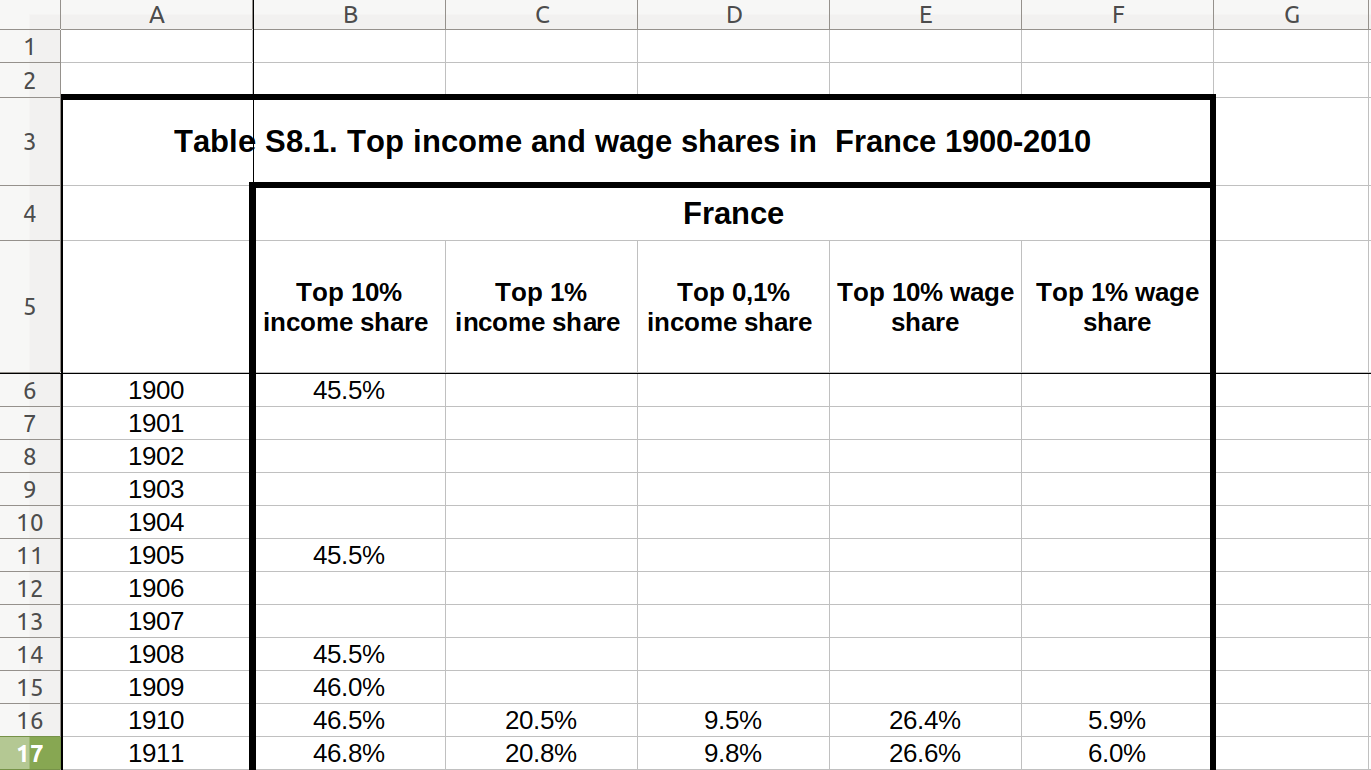
\includegraphics[width=\linewidth]{ch_data_wrangling/messy.png}
  \caption{Data on top incomes as provided in Piketty (2014; digital appendix)}\label{fig:messy}
\end{figure}

In order to perform our visualization, we want a data set containing a single measurement column (percentage share),
and a row for each year-country-type combination, i.e. one row for wage inequality in 1910 in the U.S..
One of the most important skills in computational social science (and data-driven analysis in general) is
understanding which series of generally small steps are needed to go from one data format to the other.
Although there is not a fixed set of steps that are always needed, the steps to get from the raw data visualized in \reffig{messy} to a `tidy' data set are fairly typical:

\begin{enumerate}
  \item Input: Read the data into data frames. In this case, reading from an excel sheet and skipping the extra header rows
  \item Reshape: Pivoting the data into long format
  \item Normalize: Normalize names, value types, etc. In this case, also separate a header like ``Top 1\% income share'' into income type (income, wage) and percentile (10\%, 1\%, etc)
  \item Filter: Filter for the desired data
  \item Analyze: Create the visualization
\end{enumerate}

Fortunately, These steps have been discussed before: reading csv data in \refsec{readdata}; pivot to long data in \refsec{pivot};
add a column in \refsec{calculate}; joining data in \refsec{join}; and visualizing in \refchap{visualize}.

\refex{excel} shows how to perform the first three steps for the U.S. case.
First, we use the \pkg{readxl} (R) and \pkg{xlrd} (Python) to read a sheet from an excel file into a data frame,
manually specifying the number of header and footer rows to skip.
Then, we pivot the columns into a
The missing step, splitting a header into two columns, is done using \fn{separate} (R) and \fn{split} (Python). 

\begin{ccsexample}
  \doublecodex{ch_data_wrangling/excel1}
  \codexoutputtable{ch_data_wrangling/excel1.r}
  \doublecodex{ch_data_wrangling/excel2}
  \codexoutputpng{ch_data_wrangling/excel2.py}
  \caption{Dealing with `messy' data}\label{ex:excel}
\end{ccsexample}



\setcounter{chapter}{7}
\chapter{Exploratory data analysis}
\label{chap:eda}

This chapter explains how to use data analysis and visualization techniques to understand and communicate the structure and story of our data.  It includes how to conduct exploratory statistics and data visualization in R and Python, and introduces unsupervised machine learning for clustering and dimensionality reduction to group similar cases or to decrease the number of features in a dataset.

\section{Simple exploratory data analysis}
\label{sec:simpleeda}

Now that you are familiar with data structures (\refchap{filetodata}) and data wrangling (\refchap{datawrangling}) you are probably eager to get some real insights of your data beyond the basic techniques we briefly introduced in \refchap{fundata}.

As we outlined in \refchap{introduction}, the computational analysis
of communication can be both bottom-up or top-down, inductive or
deductive.  Just as in traditional research methods \cite[for an
  overview, see, for example,][]{Bryman2012}, sometimes, an inductive
bottom-up approach is a goal in itself: After all, explorative
analyses are invaluable for generating hypothesis that can be tested
in follow-up research. But even when you are conducting a deductive,
hypothesis-testing study, it is a good idea to start by
\emph{describing} your dataset using the tools of exploratory data
analysis to get a better picture of your data. In fact, we could even
go as far as saying that obtaining descriptives like frequency tables,
cross-tabulations, and summary statistics (mean, median, mode, etc.)
is always necessary, even if your research questions or hypotheses
require further complex analysis. For the computational analysis of
communication, a significant amount of time may actually be invested
at this stage.

Exploratory data analysis (EDA), as originally conceived by \citet{tukey1977exploratory}, can be a very powerful framework to prepare and evaluate data, as well as to understand its properties and generate insights at any stage of your research.
It is mandatory to do some EDA before any sophisticated analysis to know if the data is clean enough, if there are missing values and outliers, and how the distributions are shaped.
Furthermore, before making any multivariate or inferential analysis we might want to know the specific frequencies for each variable, their measures of central tendency, their dispersion, and so on. We might also want to integrate frequencies of different variables into a single table to have an initial picture of their interrelations.

To illustrate how to do this in R and Python, we will use existing representative survey data to analyze how the demographics of Europeans citizens and relate to support the arrivalof  either migrants or refugees to the continent. The Eurobarometer (freely available at the Leibniz Institute for the Social Sciences -- GESIS) contains these specific questions since 2015. We might pose questions about the variation of a single variable or also describe the covariation of different variables to find patterns in our data. In this section, we will compute basic statistics to answer to these questions and in the next section we will visualize them by plotting \textit{within} and \textit{between} variables behaviours of a selected group of features of the Eurobarometer conducted in November 2017 to 33,193 Europeans. 

For most of the EDA we will use \pkg{tidyverse} in R and \pkg{pandas} as well \pkg{numpy} and \pkg{scipy} in Python. After loading a clean version of the survey data\footnote{Original data ZA6928\_v1-0-0.csv was cleaned and prepared for the exercise. The preparation of the data are in the notebooks cleaning\_eurobarometer\_py.ipynb and cleaning\_eurobarometer\_r.ipynb.}  stored in a cvs file (using the \pkg{tidyverse} function \fn{read\_csv} in R and the \pkg{pandas} function \fn{read\_csv} in R), checking the dimensions of our dataframe (33193 x 17), we probably want to get a global picture of each of our variables by getting a frequency table. This table shows the frequency of different outcomes for every case in a distribution. This means that we can know how many cases we have for each number or category in the distribution of every variable, which is useful to have an initial understanding of our data.

\begin{feature}
  \textbf{pandas versus pure numpy/scipy} In this book, we use pandas
  dataframes a lot: they make our lifes easier compared to native
  datatypes (\refsec{datatypes}), and they already integrate a lot of
  functionality of underlying math and statistics packages such as
  \pkg{numpy} and \pkg{scipy}. However, you do not have to force your
  data into a datatype if a different structure makes more sense in
  your script. \pkg{numpy} and \pkg{scipy} will happily calculate
  mean, media, skewness, and kurtosis of the values in a list, or the
  correlation between two lists. It's up to you.
\end{feature}


\pyrex[output=both,caption=Load data from Eurobarometer survey and select some variables]{chapter08/load}
		
Let us first get the distribution of the categorical variable \textit{gender} by creating tables that include absolute and relative frequencies. The frequency tables (using the \fn{dplyr} functions \fn{group\_by} and \fn{summarise} in R, and \pkg{pandas} function \fn{value\_counts} in Python) reveales that 17,716 (53.38\%) women and 15,477 (46.63\%) men answered this survey. We can do the same with the level of support of refugees [\textit{support\_refugees}] (\textit{To what extent do you agree or disagree with the following statement: Our country should help refugees}) and obtain that 4,957 (14.93\%) persons totally agreed with this statement, 12,695 (38.25\%) tended to agree, 5,931 (16.24\%) tended to disagree and 3,574 (10.77\%) totally disagreed. 

\begin{ccsexample}
\doublecodex{chapter08/frequency}
\codexoutputtable[Absolute and relative frequencies of gender:]{chapter08/frequency.r}
\doublecodex{chapter08/frequency2}
\codexoutputtable[Absolute and relative frequencies of support of refugees:]{chapter08/frequency2.r}
\caption{Absolute and relative frequencies of support of refugees and gender}
\end{ccsexample}


Before diving any further into any \textit{between} variables analysis, you might have noticed that there might be some missing values in the data. These values represent an important amount of data in many real social and communication analysis (just think that you cannot be forced to answer to every question in a telephone or face-to-face survey!). From a statistical point of view, we can have many approaches to address missing values that go from drop either the rows or columns that contain any of them, to compensate those values doing imputation (predicting which would the value based on its relation with other variables), as we did in \refsec{calculate} by replacing the missing values with the column mean. It goes beyon this chapter to explain all the imputation methods (and, in fact, mean imputation has some serious drawbacks when used in subsequent analysis), but at least we need to know how to identify the missing values in our data and how to drop the cases that contain them from our dataset.

In the case of the variable \textit{support\_refugees} we can count its missing data (6,576 cases) with base R function \fn{is.na} and the pandas method \fn{isna}\footnote{If missing values are not corrected declared (e.g. using strings or numbers such as 999) we should first transform the initial values into proper missing values using the \pkg{tidyverse} function \fn{na\_if} in R and the \pkg{numpy} object \fn{nan} in Python. We conducted did this when cleaning the original Eurobarometer dataset for you.}.  Then we may decide to drop all the records that contain these values in our dataset using \pkg{tydyr} function \fn{drop\_na} in R and \pkg{pandas} function \fn{dropna} in Python to drop the records\footnote{We may also use: dropna(axis='columns') if you want to drop columns instead of rows.}. By doing this we can have a cleaner dataset and continue more sophisticated EDA with cross-tabulation and summary statistics for group of cases.	

\pyrex[output=both,caption=Drop missing values]{chapter08/na}

Now let us crosstabulate the \textit{gender} and \textit{support\_refugees} to have an initial idea of how the relation between these two variables might be. With this purpose we create a contingency table or cross-tabulation to get the frequencies in each combination of categories (using \pkg{dplyr} functions \fn{group\_by}, \fn{summarise} and \fn{spread} in R, and \pkg{pandas} function \fn{crosstab} in Python). From this table you can easily get that 2,178 women totally supported to help refugees and 1,524 men totally did not.  Furthermore, other interesting questions about our data might now arise if we compute summary statistics for group of cases (using again \pkg{dplyr} functions \fn{group\_by}, \fn{summarise} and \fn{spread}, and base \fn{mean} in R; and \pkg{pandas} function \fn{groupby} and base \fn{mean} in Python). For example, you might wonder what are the average ages of women that totally supported (52.42) or not (53.2) to help of refugees.  This approach will open a huge amount of possible analysis by grouping variables and estimating different statistics beyond the mean, such as count, sum, median, mode, minimum or maximum, among others.

%Check why tables outputs in R are not supported well
\pyrex[output=both,caption=Cross tabulation of support of refugees and gender\, and summary statistics]{chapter08/cross}


\section{Visualizing data}
\label{sec:visualization}


Data visualization is a powerful technique for both understanding data yourself and communicating the story of your data to others. Based on \pkg{ggplot2} in R and \pkg{matplotlib} and \pkg{seaborn} in Python, this section covers histograms, line and bar graphs, scatterplots and heatmaps. It touches on combining multiple graphs, communicating uncertainty with boxplots and ribbons, and plotting geospatial data.  In fact, visualizing data is an important stage in both EDA and advanced analytics, and we can use graphs to obtain important insights about our data. For example, if we want to visualize the age and the support of refugees of European citizens, we can plot a histogram and a bar graph, respectively. 


\subsection{Plotting frequencies and distributions}
In the case of nominal data, the most straightforward way to visualize them is to simply count the frequency of value and then plot them as a bar chart. For instance, when we depict the support to help refugees (\refex{bar}) you can quickly get that the option ``tend to agree'' is the most frequently voiced answer.

\pyrex[output=py,format=png,caption=Barplot of support of refugees]{chapter08/bar}

If we have continous variables, however, having such a bar chart would lead to too many bars: we may loose oversight (and creating the graph may be resource-intensive). Instead, we want to group the data into \emph{bins}, like age groups.
Hence, a histogram is used to examine the distribution of a continuous variable (\pkg{ggplot2} function geom\_histogram in R and \pkg{pandas} function \fn{hist} in Python) and a graph bar to inspect the distribution of a categorical one (\pkg{ggplot2} function geom\_bar() in R and \pkg{matplotlib} function \fn{plot} in Python). In \refex{hist} you can easily notice the shape of the distribution of the variable age, with many values close to the average and a slightly bigger tail to the right (not that far from the normal distribution!).  

\pyrex[output=py,format=png,caption=Histogram of Age]{chapter08/hist}

Another way to show distributions is using bloxplots, which are powerful representations of the distribution of our variables through the use of quartiles that are marked with the 25th, 50th (median) and 75th percentiles of any given variable. By examining the lower and upper levels of two or more distributions you can compare their variability and even detect possible outliers. You can generate multiple boxplots to compare the ages of the surveyed citizens by country and quickly get that in term of age the distributions of Spain and Greece are quite similar, but we can detect some differences between Croatia and the Netherlands. In R we use the base function \fn{geom\_boxplot}, while in Python we use the \pkg{seaborn} function \fn{boxplot}.

\pyrex[output=py,format=png,caption=Bloxplots of age by country]{chapter08/boxplots}




\subsection{Plotting relationships}

After having inspected distributions of single variables, you may want to check how two variables are related. We are going to discuss two ways of doing so: plotting data over time, and scatterplots to illustrate the relationship between two continous variables.

The Eurobarometer collects data during 15 days (in the example from November 5 to 19, 2017) and you may wonder if the level of support to refugees or even to general migrants changes over the time. This is actually a simple time series and you can use a graph line to represent it. Firstly you must use a numerical variable for the level of support (\emph{support\_refugees\_n}, which ranges from 1 to 4, being 4 the maximum support) and group it by day in order to get the average for each day. In the case of R, you can plot the two series using the base function \fn{plot}, or you can use the \pkg{ggplot2} function \fn{geom\_line}. In the case of Python you can use the \pkg{matplotlib} function \fn{plot} or the \pkg{seaborn} function \fn{lineplot}. To start, \refex{line} shows how to create a graph for the average support of refugees by day.

\pyrex[output=py,format=png,caption=Graph line of average support of refugees by day]{chapter08/line}

%\pyrex[output=py,format=png,caption=Graph line of average support of migrants by day]{chapter08/line2}

To also plot the support for migrants, you can combine multiple subgraphs in a single plot,
giving the reader a broader and more comparative perspective (\refex{combine2}).
In R, the \fn{geom\_line} also takes a color aesthetic, but this requires the data to be in long format.
So, we first reshape the data and also change the factor labels to get a better legend (see \refsec{pivot}).
In Python, you can plot the two lines as separate figures figures and add the \pkg{pyplot} function \fn{show} to display an integrated figure.

\pyrex[output=py,format=png,caption=Plotting multiple lines in one graph]{chapter08/combine2}

Alternatively, you can create multiple subplots, one for each group that you want to show (\refex{combine}).
In \pkg{ggplot} (R), you can use the \fn{facet\_grid} function to automatically create subplots that each show one of the groups. In the case of Python you can use the \pkg{matplotlib} function \fn{subplots} that allows you to configure multiple plots in a single one.

\pyrex[output=py,format=png,caption=Creating subfigures)]{chapter08/combine}

Now if you want to explore the possible correlation between the average support to refugees (\texttt{mean\_support\_refugees\_by\_day}) and the average support to migrants by year (\texttt{mean\_support\_migrants\_by\_day}), you might need a scatterplot, which is a better figure to visualize the type and strength of this relationship \pkg{scatter}. 

\pyrex[output=py,format=png,caption=Scatterplot of average support of refugees and migrants by year]{chapter08/scatter}

A scatterplot uses dots to depict the values of two variables in a Cartesian plane (with coordinates for the axes X and Y). You can easily plot this figure in R using the \pkg{ggplot2} function \fn{geom\_point} (and \fn{geom\_smooth} to display a regression line!), or in Python using \pkg{seaborn} function \fn{scatterplot} (\fn{lmplot} for including the regression line as shown in \pkg{scatter2}). 

\pyrex[output=py,format=png,caption=Scatterplot with regression line]{chapter08/scatter2}

Looking at the dispersion of points in the provided example you can infer that there might be a positive correlation between the two variables, or in other words, the more the average support to refugees the more the average support to migrants over time.

We can check and measure the existence of this correlation by computing the Pearson correlation coefficient or Pearson's \emph{r}, which is the most known estimator for a correlation problem. As you probably remember from your statistics class, a correlation refers to a relationship between two continuous variables and is usually applied to measure linear relationships (although there are also exists nonlinear correlation coefficients, such as Spearman's $\rho$). Specifically, Pearson's $r$  measures the linear correlation between two variables (\emph{X} and \emph{Y}) producing a value between -1 and +1, where 0 depicts the absence of correlation and values near to 1 a strong correlation. The signs (+ or -) represent the direction of the relationship (being positive if two variables variate in the same direction, and negative if they variate in the opposite direction). The correlation corefficient is usually represented with \emph{r} or the Greek letter $\rho$ and mathematically expressed as:

$$
  r =
  \frac{ \sum_{i=1}^{n}(x_i-\bar{x})(y_i-\bar{y}) }{%
        \sqrt{\sum_{i=1}^{n}(x_i-\bar{x})^2}\sqrt{\sum_{i=1}^{n}(y_i-\bar{y})^2}}
$$

You can estimate this correlation coefficient with \pkg{pandas} function \fn{corr} in Python and the base R function \fn{cor} in R. Ass shown in \refex{corr} the two variables plotted above are highly correlated with a coefficient of 0.95.

\pyrex[output=both,caption=Pearson correlation coefficient]{chapter08/corr}

Another useful representation is the heatmap. This figure can help you plot a continuous variable using a colour scale and shows its relation with another two variables.  This means that you represent your data as colours, which might be useful for understanding patterns. For example, we may wonder what is the level of support of refugees given the nationality and the gender of the individual. For this visualization, it is necessary to create a proper dataframe (\refex{pivot}) to plot the heatmap, in which each number of your continuous variable \emph{\_refugees\_n} is included in a table where each axis (x= gender, y=country) represents the categorical variables. This pivoted table stored in an object called \texttt{pivot\_data} can be generated using some of the already explained commands.

\pyrex[output=none,caption=Create a dataframe to plot the heatmap]{chapter08/pivot}  

In the first resulting figure proposed in \refex{heatmap}, the lighter the blue the greater the support in each combination of country x gender. You can see that level of support is similar in countries such as Slovenia or Spain, and is different in Czech Republic or Austria. It also seems that women have a higher level of support. For this default heatmap we can use the \pkg{ggplot2} function \fn{geom\_tile} in R and \pkg{seaborn} function \fn{heatmap} in Python.  To personalize the scale colours (i.e. a scale of blues) we can use the \pkg{ggplot2} function \fn{scale\_fill\_gradient} in R or the parameter \texttt{cmap} of the \pkg{seaborn} function \fn{heatmap} in Python. 

\pyrex[output=py,format=png,caption=Heatmap of country\, gender and support of refugees]{chapter08/heatmap}

As you have noticed, one of the goals of EDA is exploring the variance of our variables, which includes some uncertainty about their behaviour. We will introduce you to two basic plots to visually communicate this uncertainty. Firstly, ribbons and area plots can help us to clearly identify a predefined interval of a variable in order to interpret its variance over some cases. Let us mark this interval in 0.15 points in the above-mentioned plots of the average support to refugees or migrants by day, and we can see that the lines tend to converge more in the very last day and are more separated by the day 4. This simple representation can be conducted in R using the \pkg{ggplot2} function \fn{geom\_ribbon} and in Python using the parameter \texttt{ci} of the \pkg{seaborn} function \fn{lineplot}.  

\pyrex[output=py,format=png,caption=Add ribbons to the graph lines of support to refugees and migrants]{chapter08/ribbons}




\subsection{Plotting geospatial data}

Plotting geospatial data is a more powerful tool to compare countries or other regions.  Maps are very easy to understand and can have greater impact in all kind of readers, which make them a useful representation for a wide range of studies that any computational analyst has to deal with. Geospatial data is based on the specific location of any country, region, city or geographical area, marked by its coordinates, latitude and longitude, that can later build points and polygon areas. The coordinates are normally mandatory to plot any data on a map, but are not always provided in our raw data. In those cases, we must joint the geographical information we have (i.e. the name of a country) with its coordinates in order to have an accurate dataframe for plotting geospatial data. Some libraries in R and Python might directly read and interpret different kinds of geospatial information by recognizing strings such as “France” or “Paris”, but at the end they will be converted into coordinates. 

Using the very same data of our example, we might want to plot in a map the level of support to refugees of European citizens by country. Firstly, we should create a dataframe with the average level of support to refugees by country (\texttt{supports\_country}). Secondly, we must install any exiting library that provides you with accurate geospatial information. In the case of R, we recommend the package \pkg{maps} which contains the function \fn{map\_data} that helps you generate an object with geospatial information of specific areas, countries or regions, that can be easily read and plot by \pkg{ggplot2}. Even if not explained in this book, we also recommend \pkg{ggmap} in R (\cite{kahle2013ggmap}). When working with Python we recommend \pkg{geopandas} that works very well with \pkg{pandas} and \pkg{matplotlib} (it will also need some additional packages such as \pkg{descartes}).  

In \refex{map} we illustrate how to plot a world map (from existing geographical information).
We then save a partial map into the object \texttt{some\_eu\_maps} containing the European countries that participate in the survey. After we merge \texttt{supports\_country} and \texttt{some\_eu\_maps} (by region) and get a complete dataframe called \texttt{support\_map} with coordinates for each country (\refex{countries}).  
Finally, we plot it using the \pkg{ggplot2} function \fn{geom\_polygon} in R and the \pkg{geopandas} method \fn{plot} in Python (\refex{map2}). Voilà a nice and comprehensible representation of our data with a scale of colours!

\pyrex[output=py,format=png,caption=Simple world map]{chapter08/map}

\pyrex[output=none,caption=Select EU countries and joint the map with Eurobarometer data]{chapter08/countries}

\pyrex[output=r,format=png,caption=Map of Europe with the average level of support of refugees by country]{chapter08/map2}


\subsection{Other possibilities}

There are many other ways of visualizing data. For EDA we have covered in this chapter only some of the most used techniques but they might be still limited for your future work. There are many books that cover data visualisation in detail, such as \cite{tufte2006beautiful}, \cite{cairo2019charts}, and \cite{Kirk2016}. Also, there are other packages as well as getting familiar with other packages such as \pkg{shiny} in R or \pkg{bokeh} or \pkg{plot.ly} in Python, which offer a wide range of functionalities and may fit your needs. There are also many online resources, such as the Python Graph Gallery \url{https://www.python-graph-gallery.com/} and the R Graph Gallery (\url{https://r-graph-gallery.com/}, which introduce you to other useful plots, including code examples.


\section{Clustering and dimensionality reduction}
\label{sec:clustering}

So far in this chapter we have reviewed traditional statistical exploratory and visualization techniques that any social scientist must manage. However, a more computational approach in EDA is using machine learning (ML) to let our computer “learn” about our data and in turn give us more initial insights.  ML is a branch of artificial intelligence that uses algorithms to interact with data and obtain some patterns or rules that characterize that data. We normally distinguish between supervised machine learning (SML) and unsupervised machine learning (UML). The main difference between these two approaches is that in SML we give the algorithm some “examples” in order to learn from them, and in UML we just give the algorithm the whole data and ask to learn the patterns directly from it. We will cover SML in the  chapter~\ref{chap:introsml}. In this chapter, we will focus on UML as a means of finding groups and latent dimensions in our data, which can also help to reduce our number of variables. Specifically, we will use base R and Python’s \pkg{scikit-learn} to conduct k-means clustering, hierarchical clustering and principal component analysis (PCA). 

In data mining, we use clustering as a UML technique that aims to find the relationship between a set of descriptive variables (instead of finding the relationship between those descriptive features and a target variable, as in SML). By doing cluster analysis we can identify underlying groups in our data that we will call \textit{clusters}. Imagine we want to explore how European countries can be grouped based on their average support to refugees/migrants, age and educational level. We might create some \textit{a priori} groups (such as Southern vs. Northern countries), but cluster analysis would be a great method to let the data “talk” and then create the most appropriate groups for this specific case. As in all UML, the groups will come unlabelled and the computational analyst will be in charge of finding an appropriate and meaningful label for each cluster for a better communication of results. In spite of this challenge, clustering is a very powerful approach for many EDA tasks and can help the analysis to discover patterns in data.

K-means is the most known algorithm to perform cluster analysis. It is a method that takes any number of observations (cases) and group them into a given number of clusters based on the proximity of each observation to the mean of the formed cluster (centroid).  Mathematically, we measure this proximity as the distance of any given point to its cluster center, and can be expressed as

$$J = \sum_{j=1}^{k} \sum_{i=1}^{n} \big\| X_i^{(j)} - c_j \big\| ^2$$

where $ \big\| X_i^{(j)} - C_j \big\| ^2$ is the distance between the data point $X_i^{(j)}$ and the center of the cluster $c_j$.

Instead of taking the mean, some variations of this algorithm take the median (k-medians) or a representative observation, also called medoid (k-medoids or partitioning around medoids, PAM) as a way to optimize the initial method.

The first thing is to prepare a proper dataset, using only continuous variables, scaling the data (for comparability) and avoiding missing values (drop or impute). In the above example, we will use the variables support to refugees (\emph{support\_refugees\_n}), support to migrants(\emph{support\_migrants\_n}), age (\emph{age}) and educational level (number of years of education) (\emph{educational\_n}) and will create a dataframe \verb+d3+ with the mean of all theses variables for each \emph{country} (each observation will be a country). Before conducting cluster analysis, we should establish how many clusters we want to have. This is a tricky question, since you have to tell k-means how many of them you want to and there are different ways to estimate this number (besides of arbitrarily decide it!). The simplest method to obtain the optimal number of clusters is by estimating the variability within the groups for different executions of the k-means function. This means that we must run k-means for different number of clusters (i.e. 1 to 15 clusters) and then choose the number of clusters that decreases the variability maintaining the highest number of clusters. If it is confusing, don not worry!  When you generate and plot a vector with the variability, or in more technical words, the within-cluster sum of squares (WSS) obtained after each execution, it is very easy to identify the optimal number: Just look at the bend (\textit{knee} or \textit{elbow}) and you will find the point where it decreases the most and then get the optimal number of clusters (3 clusters in our example).

\pyrex[output=py,caption=Getting the optimal number of clusters]{chapter08/elbow}

Now we can finally conduct k-means. We generate 25 initial random centroids (the algorithm will choose the one that optimizes the cost). The default of this parameter is 1, but it is recommended to set it with a higher number (i.e. 20 to 50) to guaranty the maximum benefit of the method. The base R function \fn{kmeans} and \pkg{scikit-learn} function \fn{KMeans} in Python will produce the clustering. You can observe the mean (scaled) for each variable in each cluster, as well as the corresponding cluster for each observation. Using the function \fn{fviz\_cluster} of the library \pkg{factoextra} in R, or the \pkg{pyplot} function \fn{scatter} in Python, you can have a great visualization of the clusters! In the provided example you can clearly identify that the clusters correspond to Nordic countries (more support to foreigners, more education and age), Central and Southern European countries (middle support, lower education and age), and Eastern European countries (less support, lower education and age)\footnote{We can re-run this cluster analysis using k-medoids or partitioning around medoids (PAM) and get similar results (the three medoids are: Slovakia, Belgic and Denmark), both in data and visualization. In R you must install the package \pkg{cluster} than contains the function \fn{pam}, and in Python the package \pkg{scikit-learn-extra} with the function \fn{Kmedoids}.} .

\pyrex[output=py,caption=Using Kmeans to group countries based on the average support of refugees and migrants\, age and educational level]{chapter08/kmeans}

Another method to deploy cluster analysis is hierarchical clustering, which builds a hierarchy of clusters that we can visualize in a dendogram.  This algorithm has two versions: a bottom-up approach (observations begin in their own clusters), also called \textit{agglomerative}, and a top-down approach (all observations begin in one cluster), also called \textit{divisive}. We will follow the bottom-up approach in this chapter and when you will look at the dendogram you will realize how this strategy repeatedly combines the two \textit{nearest} clusters at the bottom into a larger one in the top. The distance between clusters is initially estimated for every pair observation points and then put every point in its own cluster in order to get the closest pair of points and iteratively compute the distance between each new cluster and the previous ones. This is the internal rule of the algorithm and we must choose a specific linkage method (complete, single, average or centroid or ward). In the example we will use the function \fn{hcut} of the package \pkg{factoextra} in R and \pkg{scikit-learn} function \fn{AgglomerativeClustering} in Python, to compute the hierarchical clustering. We can then plot the dendogram  with base R function \fn{plot} and \pkg{scipy} (module \texttt{cluster.hierarchy}) function \fn(dendogram) in Python. The summary of the initial model suggest us 2 clusters (size=2) but by looking at the dendogram you can choose the number of clusters you want to work with by choosing a height (for example 4 to get 3 clusters). 

\pyrex[output=py,caption=Using hierarchical clustering to group countries based on the average support of refugees and migrants\, age and educational level]{chapter08/hc}

If you re-run the hierarchical clustering for 3 clusters and visualize it you will get a graph similar to the one produced by k-means!

\pyrex[output=py,caption=Re-run hierarchical clustering with 3 clusters]{chapter08/hc3}

Finally, we will cover principal component analysis (PCA). This unsupervised method is useful to reduce the dimensionality of your data by creating new uncorrelated variables or \textit{components} that describe the original dataset. PCA uses lineal transformation to create principal components that are ordered by the level of explained variance (the first component will catch the largest variance). We will get as many principal components as number of variables we have in the dataset, but when we look at the cumulative variance we can easily select only few of these components to explain most of the variance and thus work with a smaller and summarised dataframe that might be more convenient for many tasks (i.e. those that require avoiding multicollinearity or just need to be more computationally efficient). By simplifying the complexity of our data we can have a first understanding of how our variables are related and also of how our observations might be grouped. All components have specific loads for each original variable, which can tell you how the old variables are represented in the new components. This statistical technique is especially useful in EDA when working with high dimensional datasets but it can be used in many other situations.  

The mathematics behind PCA can be  relatively easy to understand. However, for the sake of simplicity, we will just say that in order to obtain the principal components the algorithm firstly has to compute the mean of each variable and then compute the covariance matrix of the data. This matrix contains the covariance between the elements of a vector and the output will be a square matrix with identical number of rows and columns, corresponding to the total number of dimensions of original dataset. Specifically, we can calculate the covariance matrix of the variables \emph{X} and \emph{y} with the next formula

$$cov_{x,y}=\frac{\sum_{i=1}^{N}(x_{i}-\bar{x})(y_{i}-\bar{y})}{N-1}$$

Secondly, using the covariance matrix the algorithm computes the eigenvectors and their corresponding eigenvalues, and then drop the eigenvectors with the lowest eigenvalues. With this reduced matrix it transforms the original values to the new subspace in order to obtain the principal components that will synthesize the original dataset.

Let us now conduct a PCA over the Eurobarometer data.  In the provided example we will re-use the sub dataframe \emph{d3} containing the means of 4 variables (support to refugees, support to migrants, age and educational level) for each of the 30 European countries (30 x 4). The question is if we can have a new dataframe containing less than 4 variables but that explain most of the variance, or in other words, that represent well our original dataset with less dimensions. As long as our features are usually measured in different scales, it is normally suggested to center (to mean 0) and scale (to standard deviation 1) the data. We can perform the PCA in R using the base function \fn{prcomp} and in Python using the function \fn{PCA} of the module \texttt{decomposition} of \pkg{scikit-learn}. 

\pyrex[output=py,caption=Principal component analysis (PCA) of a dataframe with 30 records and 4 variables]{chapter08/pca}

The generated object with the PCA contains different elements (in R "sdev",     "rotation", "center",  "scale" and   "x") or attributes in Python (components\_, explained\_variance\_, explained\_variance\_ratio, singular\_values\_, mean\_, n\_components\_, n\_features\_, n\_samples\_ and noise\_variance\_). In the resulting object we can see the values of 4 principal components of each country, and the values of the loadings, technically called \textit{eigenvalues}, for the variables in each principal component. In our example we can notice that support to refugees and migrants are more represented on PC1, while age and educational level on PC2. If we plot the first two principal components (using base function \fn{biplot} in R and and ad hoc function created with \pkg{pyplot} in Python) we can clearly see how the variables are associated with either PC1 or with PC2 (we might also want to plot any pair of the four components!). But we can also get a picture of how countries are grouped based only in this two new variables.

\pyrex[output=py,caption=Plot PC1 and PC2]{chapter08/plot_pca}

So far we are not sure of how many components are enough to accurately represent our data, so we need to know how much variance (which is the square of the standard deviation) is explained by each component. We can get the values and plot both the proportion of explained variance and the cumulative explained variance. We get that the first component explain 57.85\% of the variance, the second 27.97\%, the third 10.34\% and the fourth just 3.83\%. 

\pyrex[output=py,caption=Proportion of variance explained]{chapter08/prop}

When we plot the cumulative explained variance it is easy to identify that with just the two first components we explain 88.82\% of the variance. It might now seem a good deal to reduce our dataset from 4 to 2 variables, or let’s say half of the data, but retaining most of the original information.

\pyrex[output=py,caption=Cumulative explained variance]{chapter08/acum}

And what if we want to use this PCA and deploy a clustering (as explained above) with just these two new variables instead of the four original ones?  Just repeat the k-means procedure but now using a new smaller dataframe selecting PC1 and PC2 from the PCA. After estimating the optimal number of clusters (3 again!) we can compute and visualize the clusters, and get a very similar picture to the one obtained in the previous examples, with little differences such as the change of cluster of the Netherlands (more similar now to the Nordic countries!). 

\pyrex[output=py,caption=Combining PCA to reduce dimensionality and k-means to group countries]{chapter08/new}

This last exercise is a good example of how to combine different techniques in EDA. In the next chapter (chapter~\ref{chap:introsml}) we will continue explaining machine learning, but we will focus on supervised methods that will be of mandatory use for many computational analyses of both structured and unstructured data.





\setcounter{chapter}{8}
\chapter{Introduction to Statistical Modeling and Supervised Machine Learning}
\label{chap:introsml}
In this chapter, we introduce the basic concepts and ideas behind
machine learning.  We will outline how machine learning relate to
traditional statistical approaches that you already might now (and as
you will see, there is a lot of overlap), present different types of
models, and discuss how to validate them.

In a later chapter (Chapter~\ref{chap:text}), we will then
specifically apply the knoweldge you gained from this chapter to the
analysis of textual data, arguably one of the most interesting tasks
in the computational analysis of communication.

In this chapter, we mostly focus on \emph{supervised} machine learning
-- a form of machine learning, where we aim to predict a variable
that, for at least a part of our data, is known. To illustrate the
idea, imagine that you are interested in predicting the gender based
on Twitter biographies. You determine the gender for some of the
biographies yourself and hand these examples over to the computer. The
computer ``learns'' from your examples, and can then be used to
predict the gender for other twitter biographies for which you do not
know the gender.

In unsupervised machine learning, in contrast, you do not have such
examples. We have discussed some of such techniques in [ADD REFERENCE
  TO EXPLORATIVE DATA CHAPTER], in particular cluster analysis and
principal component analysis (PCA)/singular value decomposition (SVD).
Later, in chapter [ADD REFERENCE TO TOPIC MODELLING CHAPTER], we will
discuss topic models, an unsupervised method to extract so-called
topics from textual data.

Even though both approaches can be combined (for instance, one could
first reduce the amount of data using SVD, and then predict some
outcome), they can be seen as fundamentally different, also from a
theoretical and conceptual point of view.  Unsupervised machine
learning is a bottom-up approach and corresponds to an inductive
reasoning: you do not have a hypothesis of, for instance, which topics
are present in a corpus of text; you rather let the topics emerge from
the data.  Supervised machine learning, in contrast, is a top-down
approach and can be seen as more deductive: you define a priori which
topics to predict.

Both supervised and unsupervised approaches are widely used in the computational analysis of communication, and you will meet them across the book.
In this chapter, however, we will focus on supervised learning.

\section{Statistical modeling and prediction}
\label{sec:prediction}
Machine learning, many people joke, is nothing else than a fancy name
for statistics.  And, in fact, there is some truth to this: If you say
``logistic regression,'' this will sound familiar to both
statisticians and machine learning practitioners.  Hence, it does not
make much sense to distinguish between statistics on the one hand and
machine learning on the other hand.

Still, there are some differences between traditional statistical
approaches that you may have learned about in your statistics classes
and the machine learning approach, even if they use some of the same
mathematical tools. One may say that  the focus is a different
one, and the objective we want to achieve may differ.

Let us illustrate this with an example.
\texttt{mediause.csv}\footnote{You can download the file from
  \url{http://cssbook.nl/d/mediause.csv}} contains a few columns from
survey data on how many days per week respondents turn to different
media types (\emph{radio}, \emph{newspaper}, \emph{tv} and \emph{internet}) in order to follow the news\footnote{For a detailed
  description of the dataset, see \citet{Trilling2013phd}.}. It also
contains their \emph{age} (in years), their \emph{gender} (coded as female = 0, male = 1), and their \emph{education} (on a 5-point scale).

A straightforward question to ask is how far the
sociodemographic characteristics of the respondents explain their
media use.  Social scientists would typically approach this question
by running a regression analysis.  Such an analysis tells us how some
independent variables $x_1, x_2 \ldots x_n$ can explain $y$.  In an
ordinary least square regression (OLS), we would estimate $y=\beta_0 +
\beta_1 x_1 + \beta_2 x_2 + \ldots + \beta_n x_n$.

In a typical social-science paper, we would then interpret the coefficients
that we estimated, and say something like: When $x_1$ increases by one unit,
$y$ increases by $\beta_1$.
We sometimes call this ``the effect of $x_1$ on $y$'' (even though, of course,
it depends on the study design weather the relationship can really be interpreted
as a causal effect).
Additionally, we might look at the explained variance $R^2$, to assess how good the model fits our data. In \refex{ols} we use this regression approach to model the relationship of \emph{age} and \emph{gender} over the number of days per week a person reads a \emph{newspaper}. We fit the linear model using the \pkg{stats} function \fn{lm} in R and the \pkg{statsmodels} (module formula.api) function \fn{ols} in Python.

\pyrex[output=py, caption=Obtaining a model through estimating an OLS regression]{chapter09/ols}

Most traditional social-scientific analyses stop after reporting and
interpreting the coefficients of \emph{age} ($\beta = 0.0676$) and \emph{gender} ($\beta = -0.0896$), as well as the total explained variance (19\%) of such a model for our dependent variable \emph{newspaper}.
But we can go a step further. Given that we have already estimated our
regression equation, why not use it to do some \textit{prediction}?

We have just estimated that

$\textrm{newspaperreading} = -0.0896 + 0.0676 \cdot \textrm{age} + 0.1767 \cdot \textrm{gender}$

By just filling in the values for a 20 year old man, or a 40 year old
woman, we can easily calculate the expected number of days such a
person reads the newspaper per week, \emph{even if no such person
  exists in the original dataset}.

We learn that

$\hat{y}_{man20} = -0.0896 + 0.0676 \cdot 20 + 1 \cdot 0.1767 = 1.4391$

$\hat{y}_{woman40} = -0.0896 + 0.0676 \cdot 40 + 0 \cdot 0.1767 = 2.6144$

This was easy to do by hand, but of course, we could do this automatically for a large and essentially unlimited number of cases.
This could be as simple as shown in \refex{olspredict}.

\pyrex[output=py, caption=Using the OLS model we estimated before to predict the dependent variable for new data where the dependent variable is unknown.]{chapter09/olspredict}

In doing so, we shift our attention from the interpretation of coefficients to the prediction of the dependent variable for new, unknown cases. We do not
care about the actual values of the coefficents, we just need them for our prediction.
In fact, in many machine learning models, we will have so many of them that
we do not even bother to report them.

As you see, this implies that we proceed in two steps: First, we use some data
to estimate our model. Second, we use that model to make predictions.

We used an OLS regression for our first example, because it is very
straightforward to interpret and most of our readers will be familiar
with it.  However, a model can take the form of \emph{any} function,
as long as it takes some characteristics (or ``features'') of the
cases (in this case, people) as input and returns a prediction.

Using such a simple OLS regression approach for prediction, as we did in our example, can come with a couple of problems, though. One problem is that in some cases, such predictions do not make much sense. For instance, even though we know that the output should be something between 0 and 7 (as that is the number of days in a week), our model will happily predict that once a man reaches the age of 105 (rare, but not impossible), he will read a newspaper on 7.185 out of 7 days. Similarly, a one year old girl will even have a negative amount of newspaper reading. A second problem relates to the models' inherent assumptions. For instance, in our example it is quite an assumption to make that the relationships between these variables are linear – we will therefore discuss multiple models that do not make such assumptions later in this chapter. And, finally, in many cases, we are actually not interested in getting an accurate prediction of a continuous number (a \textit{regression} task), but rather in predicting a category. We may want to predict whether a tweet goes viral or not, whether a user comment is likely to contain offensive language or not, whether an article is more likely to be about politics, sports, economy, or lifestyle. In machine learning terms, these tasks are known as \textit{classification}.

In the next section, we will outline key terms and concepts in machine
learning. After that, we will discuss specific models that you
can use for different use applications.


\section{Concepts and Principles}
\label{sec:principles}

%\label{sec:supervised}
The goal of Supervised Machine Learning can be summarized in one sentence:
Estimate a model based on some data, and then use the model to predict the
expected outcome for some new cases, for which we do not know the outcome yet.
This is exactly what we have done in the introductory example in Section~\ref{sec:prediction}.

But when do we need it?

In short, in any scenario where the following two preconditions are fulfilled.
First, we have a large dataset (say, $100,000$
headlines) for which we want to predict to which class they belong to (say, whether
they are clickbait or not).
Second, for a random subset of the data (say, $2,000$ of the headlines), we already
know the class.
For example because we have manually coded (``annotated'') them.

Before we start using SML, though, we first need to have
a common terminology.
At the risk of oversimplifying matters, Table~\ref{tab:mllingo} provides a rough
guideline of how some typical machine learning terms translate to statistical
terms that you may be familiar with.

\begin{table}
\caption{Some common machine learning terms explained\label{tab:mllingo}}{
  \centering
\begin{tabularx}{\textwidth}{XX}
\toprule
machine learning lingo  & statistics lingo\\ \midrule
feature                 & independent variable  \\
label                   & dependent variable  \\
labeled dataset         & dataset with both independent and dependent variables\\
to train a model        & to estimate \\
classifier (classification)  & model to predict nominal outcomes \\
to annotate             & to (manually) code (content analysis) \\
\bottomrule
\end{tabularx}}{}
\end{table}

Let us explain them more in detail by walking through a typical SML workflow.

Before we start, we need to get a \emph{labeled dataset}.
It may be given to us, or we need to create it ourselves.
For instance, often we can draw a random sample of our data and use techniques
of manual content analysis \citep[e.g.,][]{riffe2019analyzing} to
\emph{annotate} (i.e., to manually code) the data.
You can download an example for this process (annotating the topic of news
articles) from \url{http://dx.doi.org/10.6084/m9.figshare.7314896.v1} \citep{Vermeer2018}.

It is hard to give a rule of thumb for how much labelled data you need.
It depends heavily on the type of data you have (if it is a \emph{binary} or a \emph{multi-class} classification problem), and on how evenly distributed (\emph{class balance}) they are (after all, having $10,000$ annotated headlines doesn't help you if $9,990$ are no clickbait and only $10$ are).
These reservations notwithstanding, it is fair to say that typical sizes in
our field are (very roughly) speaking often in the order of $1,000$ to $10,000$
when classifying longer texts \citep[see][]{Burscher2014},
even though researchers studying less rich data sometimes annotate larger
datasets \citep[e.g., $60,000$ social media messages in][]{vermeer2019seeing}.

Once we have established that this labelled dataset is available and
have ensured that it is of good quality, we randomly split it into two
datasets: a \emph{training dataset} and a \emph{test
  dataset}.\footnote{In Section~\ref{sec:validation}, we discuss more
  advanced approaches, such as splitting into training, validation,
  and test dataset, and cross-validation.}  We will use the first one
to train our model, and the second to test how good our model
performs. Common ratios range from 50:50 to 80:20; and especially if
the size of your labelled dataset is rather limited, you may want to
have a slightly larger training dataset at the expense of a slightly
smaller test dataset.

In \refex{preparedata}, we prepare the dataset we already used in
Section~\ref{sec:prediction} for classification by creating a
dichotomous variable (the label) and splitting it into a training and
a test dataset. We use |y_train| to denote the training labels and
|X_train| to denote the feature matrix of the training dataset;
|y_test| and |X_test| is the corresponding test dataset. We set a
so-called random-state seed to make sure that the random splitting
will be the same when re-running the code. We can easily split these datasets using the \pkg{rsample} function \fn{initial\_split} in R and the \pkg{sklearn} function \fn{train\_test\_split} in Python.

\pyrex[output=py, caption=Preparing a dataset for supervised machine learning]{chapter09/preparedata}

We now can \emph{train our classifier} (i.e., estimate our model using the
training dataset contained in the objects \texttt{X\_train} and \texttt{y\_train}). This can be as straightforward as estimating a
logistic regression equation (we will discuss different classifiers in
Section~\ref{sec:nb2dnn}).  It may be that we first need to create new
independent variables, so-called features, a step known as
\emph{feature engineering}, for example by transforming existing
variables, combining them, or by converting text to numerical word
frequencies.
\refex{nb} shows how easy it is to train a classifier using the Na\"ive Bayes algorithm with packages \pkg{caret}/\pkg{naivebayes} in R and \pkg{sklearn} in Python (this approach will be better explained in Subsection~\ref{subsec:naivebayes}).

\pyrex[output=none, caption=A simple Na\"ive Bayes classifier]{chapter09/nb}

But before we can actually use this classifier to do some useful work, we need to test how capable it actually is to predict the
correct labels, given a set of features. One might think that we could
just feed it the same input data (i.e., the same features) again and
see whether the predicted labels match the actual labels of the test
dataset.  In fact, we could do that.  But this test would not be
strict enough: After all, the classifier has been trained on exactly
these data, and therefore one would expect it to perform pretty well.
In particular, it may be that the classifier is very good in
predicting its own training data, but fails at predicting other data,
because it overgeneralizes some idiosyncrasy in the data, a phenomenon
known as overfitting (see Figure ~\ref{fig:overfit}).

\begin{figure} 
\centering
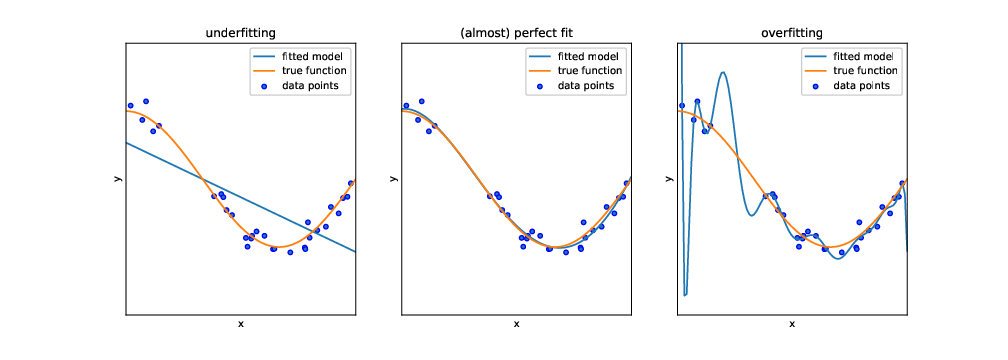
\includegraphics[width=\linewidth]{figures/ch09_overfitting}
\caption{Underfitting and overfitting. Example adapted from https://scikit-learn.org/stable/auto\_examples/model\_selection/plot\_underfitting\_overfitting.html}
\label{fig:overfit}
\end{figure}

Instead, we use the features of the \emph{test dataset} (stored in the objects  \texttt{X\_test} and \texttt{y\_test})  as input for
our classifier, and evaluate in how far the predicted labels match the
actual labels.  Remember: the classifier has at no point in time seen
the actual labels.  Therefore, we can in fact calculate how often the
prediction is right.\footnote{We assume here that the manual annotation
  is always right; an assumption that one may, of course,
  challenge. However, in the absence of any better proxy for reality,
  we assume that this manual annotation is the so-called \emph{gold
    standard} that reflects the \emph{ground truth} as closely as
  possible, and that it by definition cannot be outperformed. When creating the manual annotations, it is therefore important to safeguard their quality. In particular, one  should calculate and report some reliability measures, such as the \emph{intercoder reliability} which tests the degree of agreement between two or more annotators in order to check if our classes are well defined and the coders are doing their work correctly.}

\pyrex[output=py, caption=Calculating precision and recall]{chapter09/classificationreport}

As shown in \refex{classificationreport}, we can create a \emph{confusion matrix} (generated with \pkg{caret} function \fn{confusionMatrix} in R and \pkg{sklearn} function \fn{confusion\_matrix} in Python), and then estimate two measures: \emph{precision} and \emph{recall} (using base R calculations in R and \pkg{sklearn} function \fn{classification\_report} in Python). In a binary classification, the \emph{confusion matrix} is a useful table in which each column usually represents the number of cases in a predicted class, and each row the number of cases in the real or actual class. With this matrix (see \reffig{matrix}) we can then estimate the number of \emph{true positives} (TP) (correct prediction), \emph{false positives} (FP) (incorrect prediction), \emph{true negatives} (TN) (correct prediction) and \emph{false negatives} (FN) (incorrect prediction).


\begin{figure} 
\centering
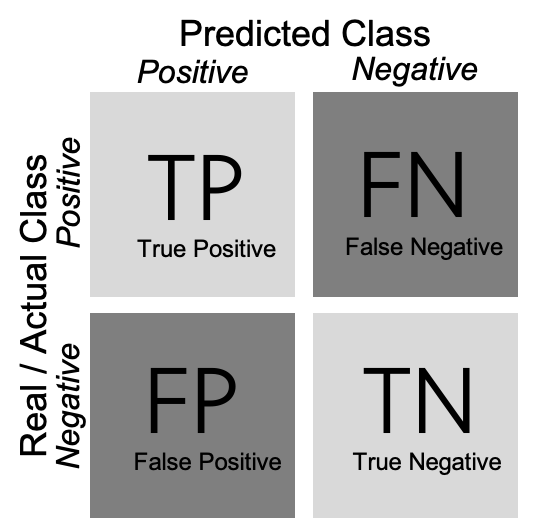
\includegraphics[width=\linewidth]{figures/ch09_matrix}
\caption{Visual representation of a confusion matrix}
\label{fig:matrix}
\end{figure}

For a better understanding of these concepts, imagine that we build a sentiment classifier, that predicts -- based on the
text of a movie review -- whether it is a positive review or a
negative review. Let us assume that the goal of training this classifier is to build an app that recommends the user only good movies. There are two things
that we want to achieve: We want to find as many positive films as possible (recall), but we also want that the selection we found
\emph{only} contains positive films (precision).

Precision is calculated as $\frac{TP}{TP+FP}$, where TP are true
positives and FP are false positives. For example, if our classifier
retrieves 200 articles that it classifies as positive films, but only
150 of them indeed are positive films, then the precision is
$\frac{150}{150+50} = \frac{150}{200} = 0.75$.

Recall is calculated as $\frac{TP}{TP+FN}$, where TP are true
positives and FN are false negatives. If we know that the classifier
from the previous paragraph missed 20 positive films, then the recall
is $\frac{150}{150+20} = \frac{150}{170}= 0.88$.

In other words: Recall measures how many of the cases we wanted to
find we actually found. Precision measures how much of what we have
found actually is correct.

Often, we have to make a trade-off between precision and recall. For
example, just retrieving \emph{every} film would give us a recall of
1.0 (after all, we didn't miss a single positive film). But on the
other hand, we retrieved all the negative films as well, so precision
will be extremely low. It can depend on the task at hand whether
precision or recall is more important. In
Section~\ref{sec:validation}, we discuss this tradeoff in detail, as well as other metrics such as \emph{accuracy}, \emph{f1-score} or the \emph{area under the curve} (AUC).


\section{From Na\"{i}ve Bayes to Deep Neural Networks}
\label{sec:nb2dnn}


\section{Validation and best practices}
\label{sec:validation}
\subsection{Finding a balance between precision and recall}
\label{sec:balance}

In the previous sections, we have learned how to fit different models:
Na\"ive Bayes, logistic regressions, support vector machines, and
random forests.  We have also had a first look at confusion matrices,
precision, and recall.

But how do we find the best model? ``Best'', here, should be read as
``best for our purposes'' -- some models may be bad, and some may be
good, but which one is really the best may depend on what matters most
for us: Do we care more about precision or about recall? Are all
classes equally important to us?  And of course, other factors, such
as explainability or computational costs may factor into our decision.
 
But in any event, we need to decide which metrics to focus on.  We can
then either manually inspect them and look, for instance, which model
has the highest \emph{accuracy}, or the best balance of precision and recall,
or a recall higher than some threshold you are willing to accept.

If we build a classifier to distinguish spam messages from legitimate
messages, we could ask the following questions:
\begin{description}
\item[Precision] Which percentage of what our classifier predicts to be
  spam really is spam?
\item[Recall]{What percentage of all spam messages has our classifier
  found?}
\item[Accuracy]{In which percentage of all cases was our classifier
  right?}
\end{description}

We furthermore have:
\begin{description}
\item[F1-score]{The harmonic mean of precision and recall: $F_1 = 2
  \cdot \frac{precison \cdot recall}{precison + recall}$}
\item[AUC]{The AUC (Area under Curve) is the area under the curve that
  one gets when plotting the True Positive Rate (TPR) against the
  False Positive Rate (FPR) at various threshold settings. A perfect
  model will receive a value of 1.0, while random guessing between two
  equally probable classes will result in a value of 0.5}
\item[Micro- and macroaverage]{Especially when we have more than two
  classes, we can calculate the average of measures such as precision,
  recall, or f1-score. We can do so based on the separately calculated
  measures (macro), or based on the underlying values (TP, FP, etc.)
  (micro), which has different implications in the interpretation --
  especially if the classes have very different sizes.}
\end{description}


So, which one to choose?  If we really do not want to be annoyed by
any spam in our inbox, we need a high recall (we want to find all spam
messages). If, instead, we want to be sure that we do not
accidentally throw away legitimate messages, we need a high
precision (we want to be sure that all spam really is spam).

Maybe you say: well, I want both!  You could look at the accuracy, a
very straightforward to interpret measure. However, if you get many
more legitimate messages than spam (or the other way round), this
measure can be misleading: after all, even if your classifier finds
almost none of the spam messages (it has a recall close to zero), you
still get a very high accuracy, simply because there are so many
legitimate messages. In other words, the accuracy is not a good measure when working with highly unbalanced classes.
Often, it is therefore a better idea to look at the harmonic mean of
precision and recall, the F1-score, if you want to find a model that
gives you a good compromise between precision and recall.


In fact, we can even fine-tune our models in such a way that they are
geared towards either a better precision or a better recall.
As an example, let us take a logistic regression model. It predicts a
class label (such as ``spam'' versus ``legitimate''), but it can also
return the assigned probabilities. For a specific message, we can thus
say that we estimate its probability of being spam as, say, .65.
Unless we specify otherwise, everything above .5 will then be judged
to be spam, everything below as legitimate. But we could specify a
different cutoff point: we could, for instance, decide to classify
only everything above .7 as spam. This would give us a more
conservative spam filter, with probably a higher precision at the
expense of a lower recall.

\begin{figure} 
\centering
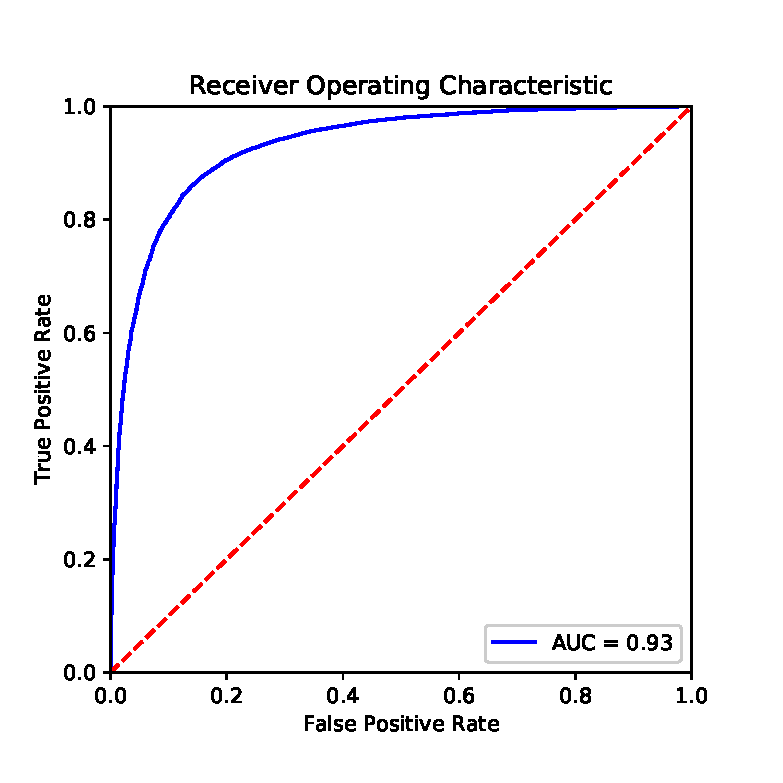
\includegraphics[width=0.4\linewidth]{figures/ch09_roccurve}
\caption{A ROC curve.}
\label{fig:roccurve}
\end{figure}

We can visualize this with a so-called ROC (reveicer operator
chraracteristic), a plot in which (Figure~\ref{fig:roccurve}) we plot
true positives against false positives at different thresholds.  A
good model extends until close to the upper left corner, and hence has
a large area under the curve (AUC).  If we choose a threshold at the
left end of the curve, we get few false positives (good!), but also
few true positives (bad!), if we go too far to the right, we get
the other extreme. So, how can we find the best spot?

One approach would be to print a table with three columns: the false
positive rate, the true positive rate, and the threshold value. You
then decide which FPR-TPR combination is most appealing to you, and
use the corresponding threshold value.

The second approach (also knwon as Yoden's J) is to find the threshold
value with the maximum distance between TPR and FPR, and use that one.

\pyrex[input=py, output=py,caption={Choosing a differnet cutoff point for predictions with logistic regression. In this case, we make a tradeoff and maximize the difference between false positive rate and true positive rate to improve the precision for the the second categegory by .12 at the expense of reducing the precision for the first category by .8.}]{chapter09/cutoffpoint}


\subsection{Train, validate, test}
\label{sec:train}

By now, we have established which measures we can use to decide which
model to use. For all of them, we have assumed that we split our
labeled dataset into two: a training dataset and a test dataset. The
logic behind it was simple: If we would calculate precision and recall
on the training data itself, our assessment would be too optimistic --
after all, our models have been trained on exactly these data, so
predicting the label isn't too hard. Assessing the models on a different
dataset, the test dataset, instead, gives us an assessment of how
precision and recall look like if haven't seen the labels earlier --
which is exactly what we want to know.

Unfortunately, if we calculate precision and recall (or any other
metric) for multiple models on the same test dataset, and use these
results to determine which metric to use, we can run into a problem:
We may avoid overfitting of our model on the training data, we may now
overfit it on the test data! After all, we could tweak our models as
long until they fit our test data perfectly, even if this makes the
predictions for other cases worse.

One way to avoid this is to split the original data into three
datasets instead of two: a training dataset, a validation dataset, and
a test dataset.  We train multiple model configurations on the
training dataset and calculate the metrics of interest for all of them
on the validation dataset.  Once we have decided on a final model, we
calculate its performance (once) on the test dataset, to get an
unbiased estimate of its performance.



\subsection{Cross-validation and grid search}
\label{sec:crossvalidation}
In an ideal world, we would have a huge labelled dataset and do not
need to worry about the decreasing size of our training dataset as we
set aside our validation and test datasets.

Unfortunately, our labelled datasets in the real world have a limited
size, and setting aside too many cases can be problematic. Especially
if you are already on a tight budget, setting aside not only a test
dataset, but also a validation dataset of meaningful size may lead to
critically small training datasets. While we have addressed the
problem of overfitting, this could lead to underfitting: We may have
removed the only examples of some specific feature combination, for
instance.

A common approach to address this issue is $k$-fold
cross-validation. To do so, we split our data into $k$ partitions,
so-called folds. We then estimate our model $k$ times, and each time
leave \emph{one} of the folds aside for validation. Hence, every fold
is exactly one time the validation dataset, and exactly $k-1$ times
part of the training data. We then simply average the results of our
$k$ values for the evaluation metric we are interested in.

If our classifier generalizes well, we would expect that our metric of
interest (e.g., the accuracy, or the f1-score, \ldots) is very similar
in all folds. ~\refex{crossval} performs a cross-validation based on
the logistic regression classifier we build above. We see that the
standard deviation is really low, indicating that there are almost no
changes between the runs, which is great.

Running the same cross-validation on our random forest, instead, would
produce not only worse (lower) means, but also worse (higher) standard
deviations, even though also here, there are no dramatic changes
between the runs.

\pyrex[input=both, output=both,caption=Crossvalidation]{chapter09/crossval}

Very often, cross-validation is used when we want to compare many
different model specifications, for example to find optimal
hyperparameters.
Hyperparameters are parameters of the model that are not estimated
from the data. These depend on the model, but could for example be the
estimation method to use, the number of times a bootstrap should be
repeated, etc. A very good example are the hyperparameters of support
vector machines (see above): It is hard to know how soft our margins
should be (the $C$), and we may also be unsure about the right kernel
(\refex{gridsearch2}), or in the case of a polinomial kernel, how many
degrees we want to consider.

Using the help function (e.g., \fn{RandomForestClassifier?} in Python),
you can look up
which hyperparameters you can specify. For a random forest classifier,
for instance, this includes the number of estimators in the model, the
criterion, and whether or not to use
bootstrapping. \refex{gridsearch}, \ref{ex:gridsearch2}, and
\ref{ex:gridsearch3} illustrate how you can automatically assess which
values you should choose.

\pyrex[input=py, output=py,caption=A simple gridsearch in Python]{chapter09/gridsearch}

\pyrex[input=py,output=py,caption=A gridsearch in Python using multiple CPUs]{chapter09/gridsearch2}

\pyrex[input=r,output=r,caption={A gridsearch in R. Note that in R, not all parameters are ``tunable'' using standard \pkg{caret}. Therefore, an exact replication of the grid searches in \refex{gridsearch} and \refex{gridsearch2} would requires either manual comparisons or writing a so-called caret extension.}]{chapter09/gridsearch3} 

\begin{feature}
    Supervised machine learning is one of the areas where you really
    see differences between Python and R. While in Python, virtually
    all you need is available via \pkg{scikit-learn}, in R, we often
    need to combine \pkg{caret} with various libraries providing the
    actual models. In contrast, all components we need for machine
    learning in Python are developed within one package, which leads
    to less friction. This is what you see in the gridsearch examples
    in this section. In scikit-learn, \emph{any} hyperparameter can be
    part of the grid, but no hyperparameter has to be.  Note that in
    R, in contrast, you cannot (at least, not easily) put any
    parameter of the model in the grid. Instead, you can look up the
    ``tunable parameters'' which \emph{must} be present part of the
    grid in the caret documentation. This means that an exact
    replication of the grid searches in \refex{gridsearch} and
    \refex{gridsearch2} is not natively supported using \pkg{caret}
    and requires either manual testing or writing a so-called caret
    extension.

    While in the end, you can find a supervised machine learning
    solution for all your use cases in R as well, if supervised
    machine learning is at the core of your project, it may save you a
    lot of cursing to do this in Python.
\end{feature}



\chapter{Processing text}
\label{chap:protext}


\begin{abstract}{Abstract}
Many data sets that are relevant for social science consist of textual data, from political discussions and newspaper archives to open-ended survey questions and reviews. This chapter gives an introduction in dealing with textual data using base R and Python, as well as packages such as \pkg{Quanteda} and \pkg{SpaCyr} in R, or \pkg{NLTK} and \pkg{SpaCy} in Python, and shows how to solve common problems encountered when reading and processing text. 
\end{abstract}

\keywords{Text representation, text cleaning, regular expressions}

\begin{objectives}
\item Understand how text is represented in the computer
\item Be able to clean up and alter text
\item Understand and be able to use regular expressions 
\end{objectives}


\section{Reading and cleaning text}
\label{sec:readtext}

When dealing with textual data, an important step is to normalize the data. Such preprocessing ensures that noise is removed, and reduces the amount of data to deal with. In \refsec{encodings} we explained how to read data from different formats, such as txt, csv or json that can include textual data, and we also mentioned some of the challenges when reading text (i.e. encoding/decoding from/to Unicode). In this section we cover typical cleaning steps such as lowercasing and removing punctuation, HTML tags and boilerplate.
 
As a computational communication scientist you will come across with many sources of text that range from electronic versions of newspapers in HTML to parliamentary speeches in PDF. Moreover, most of the contents in their original shape will include data that will not be of interest for the analysis but, instead,  will produce noise that might negatively affect the quality of the research. You have to decide which parts of the raw text should be considered for analysis and determine the shape of these contents in order to have a good input in the analytical process. 

There is not a rule of thumb that can guide you in this preprocessing stage, and it is highly likely that you will have to test different combination of steps and assess what are the best options. For example, in some cases keeping capital letters within a chat conversation or a news comment might be valuable to detect the tone of the message, but in more formal speeches transforming the whole text to lowercases would help to normalize the content. However, it is true that there some typical challenges to reduce the noise from the text.

The first thing to keep in mind is that once you load any text on R or Python you usually store this content as a \emph{character} or \emph{string} object (or you may also think of \emph{lists} or \emph{dictionaries}, but they will have strings inside anyway), which means that basic operations and conditions of this data type apply, such as indexing or slicing to access individual characters or substrings (see \refsec{datatypes}). In fact, base strings operations are very powerful to clean your text and eliminate a big amount of noise of it.  Table~\ref{tab:stringoperations} summarises some useful operations on strings in R and Python that will help you in this stage.   

\begin{table}
  \caption{\label{tab:stringoperations}Useful strings operations in R and Python to clean noise}{
  \begin{tabularx}{\textwidth}{lllll}
    \toprule
String operation      & R   & Python\\ \midrule
Count characters      & nchar(string) & len(string)  \\
Get a substring       & substr(string, start=n1, stop=n2) & string[n1:n2]            \\
Split the string into several strings   & strsplit(string, split) & split(string, split)             \\ 
Convert to lowercase  & tolower(string) & string.lower     \\ 
Convert to uppercase  & toupper(string) & string.upper     \\ 
Find and replace      & gsub("substring1","substring2",string) & string.replace('substring1','substring2') \\ 
    \bottomrule
  \end{tabularx}}{}
\end{table}

Let us apply some of these functions/methods to a simple Wikipedia text that contains HTML tags or boilerplate, punctuation and natural upper/lower case letters. Using base function \fn{gsub} in R and \fn{replace} in Python we can remove strings containing specific expressions such as \texttt{<p>} or \texttt{</b>} and include an empty space instead. We can use this same method to eliminate punctuation taking as a reference a pre-defined list of signs (\texttt{:punct:} in base R or the object \texttt{punctuation} from the library \pkg{string} in Python). In the case of converting letters from upper to lower case, we use the base R function \fn{tolower} and the string method \fn{lower} in Python. To remove unnecessary double spaces we apply the base R function \fn{trimws} and method \fn{join} in Python. \refex{clean} shows how to conduct this cleaning process.

\pyrex[output=both,caption=Cleaning text with base functions]{chapter10/clean}

It is good news that we have some extra packages that facilitate this initial stage and clean boilerplate. For instance, you can think of \pkg{stringi} in R (recommended by \citet{welbers2017text} as a better option than built-it functions) or \pkg{Beautiful Soup} in Python. \refex{cleanextra} shows how to implement these packages to remove html tags.

\pyrex[output=both,caption=Cleaning text with stringi and Beautiful Soup]{chapter10/cleanextra}

As you can notice in the R example, the package \pkg{stringi} removed the tags using the function \fn{stri\_replace\_all} and a \emph{regular expression} (which are very useful in this cleaning stage and that we will explain in the next section). We also eliminated the surrounding white spaces with the function \fn{stri\_trim}. In the case of the Python example, the library \pkg{BeautifulSoup} helps you to \emph{parse} the text with the same-name function \fn{BeautifulSoup} and then extract the text without the html tags using the function \fn{get\_text}.	

\section{Regular expressions}
\label{sec:regular}

A \concept{regular expression} or \emph{regex} is a powerful language to locate strings that conform a given pattern. For instance, we can extract usernames or email-addresses from text, or normalize spelling variations and improve the cleaning methods covered in the previous section. Specifically, regular expressions are a sequence of characters that we can use to design a pattern and then use this pattern to \emph{find} strings (identify or extract) and also \emph{replace} those strings by new ones. 

Regular expressions look complicated, and in fact they take some getting used to initially.
For example, a relatively simple (and not quite correct) expression to match an email address is \verb|[\w\.-]+@[\w\.-]+\.\w\w+|,
which doesn't look like anything at all unless you know what you are looking for.
The good news is that regular express syntax is the same in R and Python (and many other languages),
so once you learn regular expressions you will have acquried a powerful and versatile tool for text processing. 

%We will show how you can use regexes to preprocess text. The good thing is that regular expression syntax can be similar in R and Python and once you learn how to write a pattern in one language it is easy to do the same in the other.  However they are not identical! Even it is out of the scope of this book, you can trace the specific standards of each language and its different versions. You will come across with some standards of the Portable Operating System Interface (POSIX), such as the Basic Regular Expressions (BRE) or Extended Regular Expressions (ERE), or also with the Perl Compatible Regular Expressions (PCRE).  By default the R function \fn{grep} uses ERE but you can set a parameter (\verb|perl = TRUE|) to work with PCRE, and in the case of Python \fn{re} module regexes match operations similar to PCRE as a default.

%% \note{\textbf{Python: re versus regex}
%%   In python, people generally use the \pkg{re} package for regular expressions.
%%   In this book we will use the \pkg{regex} package, however.
%%   This modules has the same functions and arguments as the \pkg{re} module,
%%   but it has better support for unicode, which is very important when dealing with non-western text.
%%   However, for almost all examples you can also use the \pkg{re} module if prefered.
%%   }

In the next section, we will first review general expression syntax without reference to running them in Python or R.
Subsequently, you will see how you can apply these expression to inspect and clean texts in both languages.

\subsection{Regular expression syntax}

At its core, regular expressions are patters for matching sequences of characters.
In the simplest case, a regular letter just matches that letter, so the pattern `cat' matches the text `cat'.
Next, there are various wildcards, or ways to match different letters.
For example, the period (\verb|.|) matches any character, so \verb|c.t| matches both `cat' and `cot'.
You can place mulitple letters between square brackets to create a \concept{character class} that matches all the specified letters, so \verb|c[au]t| matches `cat' and `cut', but not `cot'.
There are also a number of pre-defined classes, such as \verb|\w| which matches `word characters' (letters, digits, and (curiously) underscores).

Finally, for each character or group of characters you can specify how often it should occur.
For example, \verb|a+| means one or more a's while \verb|a?| means zero or one a, so \verb|lo+l| matches `lol', `lool', etc.,
and \verb|lo?l| matches `lol' or `ll'.
This raises the question, of course, of how to look for actual occurrences of a plus, question mark, or period.
The solution is to \concept{escape} these special symbols by placing a backslash (\verb|\|) before them:
\verb|a\+| matches the literal text `a+', and \verb|\\w| (with a double backslash) matches the literal text `\textbackslash w'. 

Now, we can have another look at the example emails address pattern given above.
The first part, \verb|[\w\.-]| creates a character class containing word characters, (literal) periods, and dashes.
Thus, \verb|[\w\.-]+@[\w\.-]+| means one or more letters, digits, underscores, periods, or dashes, followed by an at sign,
followed by one or more letters, digits, etc.
Finally, the last part \verb|\.\w\w+| means a literal period, a word character, and one or more word characters.
In other words, we are looking for a name (possibly contining dashes or periods) before the at sign,
followed by a domain, followed by a top level domain (like \verb|.com|) of at least two characters.

In essence, thinking in terms of what you want to match and how often
you want to match it is all there is to regular expressions.
However, it will take some practice to get comfortable with turning something sensible (such as an email address) into a correct regular expression pattern.
The next subsection will explain regular expression syntax in more detail, followed by an explanation of grouping,
and in the final subsection we will see how to use these regular expressions in R and Python to do text cleaning. 

\newcommand{\fnregexnote}{\footnote{Note that this is not a full review of everything that is possible with regular expressions, but this includes the most used options and should be enough for the majority of cases. Moreover, if you descend into the more specialized aspects of regular expressions (with beautiful names such as `negative lookbehind assertions') you will also run into differences between Python, R, and other languages, while the features used in this chapter should function in most implementations you come across unless specifically noted.}}




\newcommand{\ttt}[1]{\texttt{\small{#1}}}
\newcommand{\bs}[1]{\ttt{\textbackslash#1}}

\begin{table}
  \caption{\label{tab:regex}Regular expression syntax}{
  \begin{tabularx}{\textwidth}{lllll}
    \toprule
\multicolumn{2}{l}{Function}      & Syntax   & Example & Matches    \\
    \midrule
\multicolumn{2}{l}{\textit{What to match}} \\
& All characters except for new lines   & \ttt{.} & \ttt{d.g} & \ttt{d\textbf{i}g}, \ttt{d\textbf{!}g}\\
& Word characters$^*$
  (letters, digits, \_)         & \bs{w} & \ttt{d\textbackslash{}wg} & \ttt{dig}, \ttt{dog} \\
%& Everything except word characters     & \bs{W} \\
& Digits$^*$ (0 to 9)                       & \bs{d} & \ttt{202\textbackslash{}d} & \ttt{2020}, \ttt{2021} \\
%& Everything except digits              & \bs{D} \\
& Whitespace$^*$ (space, tab, newline) & \bs{s} \\
%& Everything except whitespace	& \bs{S} \\
& Newline	& \bs{n} & \\

& Beginning of the string	& \ttt{\^{}} & \ttt{\^{}go} & \ttt{\textbf{go} {\color{gray}go go}}\\
& Ending of the string   & \ttt{\$} & \ttt{go\$} & \ttt{{\color{gray}go go} \textbf{go}} \\
& Beginning or end of word & \bs{b} & \ttt{\textbackslash{}bword\textbackslash{}b} & \ttt{{\color{gray}a} \textbf{word}\color{gray}!} \\
& Either first or second option  & \ttt{$\cdots$\textbar$\cdots$} & \ttt{cat\textbar{}dog} & \ttt{cat}, \ttt{dog}\\

\multicolumn{2}{l}{\textit{How many to match}} \\
& Zero or more & \ttt{*} & \ttt{d.*g} & \ttt{dg}, \ttt{drag}, \ttt{d = g} \\
& Zero or more (non-greedy) & \ttt{*?} & \ttt{d.*?g} & \ttt{\textbf{dog}{\color{gray}g}} \\
& One or more & \ttt{+}  & \ttt{\textbackslash{}d+\%} & \ttt{1\%}, \ttt{200\%} \\
& One or more (non-greedy) & \ttt{+?}  & \ttt{\textbackslash{}d+\%} & \ttt{{\color{gray}20}\textbf{0\%}} \\
& Zero or one  & \ttt{?} & \ttt{colou?r} & \ttt{color}, \ttt{colour} \\
& Exactly n times  & \ttt{\{n\}} & \ttt{\textbackslash{}d{\{4\}}} & \ttt{1940}, \ttt{2020} \\
& At least n times  & \ttt{\{n,\}} \\
& Between n and m times  & \ttt{\{n,m\}} \\

\multicolumn{2}{l}{\textit{Other constructs}} \\
& Groups & \ttt{($\cdots$)} & \ttt{'(bla )+'} & \ttt{'blah blah blah'} \\
& Selection of characters & \ttt{\lbrack$\cdots$\rbrack} & \ttt{d\lbrack iuo\rbrack g}& \ttt{dig}, \ttt{dug}, \ttt{dog} \\
& Range of characters in selection & \ttt{\lbrack a-z\rbrack} \\
& Everything except selection & \ttt{\lbrack\^{}...\rbrack} \\
& Escape special character & \ttt{\textbackslash{}} & \ttt{3\textbackslash{}.14} & \ttt{3.14} \\

\multicolumn{4}{l}{\textit{Unicode character properties$^\dagger$}} \\
& Letters$^*$ & \multicolumn{2}{l}{\ttt{\textbackslash{}p\{LETTER\}}} & \ttt{words}, 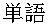
\includegraphics[height=1em]{chapter10/tango.pdf}\\
& Punctuation$^*$ &\multicolumn{2}{l}{ \ttt{\textbackslash{}p\{PUNCTUATION\}}} & . , : \\
& Quotation marks$^*$ & \multicolumn{2}{l}{\ttt{\textbackslash{}p\{QUOTATION MARK\}}} & ' ` " «  \\
& Emoji$^*$ & \multicolumn{2}{l}{\ttt{\textbackslash{}p\{EMOJI\}}} & 
\includegraphics[height=1em]{chapter10/emoji.pdf}  \\
& Specific scripts, e.g. Hangul$^*$& \multicolumn{2}{l}{\ttt{\textbackslash{}p\{HANG\}}} & 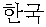
\includegraphics[height=1em]{chapter10/hangul.pdf}\\

    \bottomrule
  \end{tabularx}}{\small
    $*$ These selectors can be inverted by changing it into a capital letter. Thus, \bs{W} matches everything except word characters, and \ttt{\textbackslash{}P\{PUNCTUATION\}} matches everything except punctuation\\
    $\dagger$ See \url{https://www.unicode.org/reports/tr44/\#Property\_Index} for a full list of unucode properties. Note that when using Python, these are only available if you use \pkg{regex}, which is a drop-in replacement for the more common \pkg{re}.}
\end{table}


In \reftab{regex} you will find an overview of the most important parts of regular expression syntax.\fnregexnote
The first part shows a number of common specifiers for determining what to match, e.g. letters, digits, etc.,
followed by the quantifiers available to determine how often something should be matched.
These quantifiers always follow a specifier, i.e. you first say what you're looking for, and then how many of those you need.
Note that by default quantifiers are greedy, meaning they match as many characters as possible.
For example, \verb|<.*>| will match everything between angle brackets, but if you have something like `<p>a paragraph</p>'
it will happily match everything from the first opening bracket to the last closing bracket.
By appending a question mark (\verb|?|) to the quantifier, it becomes non-greedy.
so, \verb|<.*?>| will match the individual `<p>' and `</p>' substrings. 

The third section discusses other constructs.
\concept[Capture Groups]{Groups} are formed using parentheses \verb|()| and are useful in at least three ways. 
First, by default a quantifier applies to the letter directly before it, so \verb|no+| matches `no', `nooo', etc.
If you group a number of characters you can apply a quantifier to the group. So, \verb|that's (not)? good| matches either `that's not good' or `that's good'.
Second, when using a vertical bar (\textbar) to have multiple options, you very often want to put them into a group so you can use it as part of a larger pattern.
For example, \verb!a (great|fantastic)? victory! matches either `a victory', `a great victory', or `a fantastic victory'.
Third, as will be discussed below in \refsec{regextract}, you can use groups to capture (extract) a specific part of a string, e.g. to get only the domain part of a web address. 

The other important construct are \concept{character classes}, formed using square brackets \verb|[]|.
Within a character class, you can specify a number of different characters that you want to match, using a dash (\verb|-|) to indicate a range.
You can add as many characters as you want: \verb|[A-F0-9]| matches digits and capital letters A through F.
You can also invert this selection using an initial caret: \verb|[^a-z]| matches everything except for lowercase Latin letters.
Finally, you sometimes need to match a control character  (e.g. \verb!+!, \verb|?|, \verb|\|). Since those characters have a special meaning within a regular expressing, they cannot be used directly. The solution is to add a backslash (\verb|\|) behind them to \concept{escape} them:
\verb|.| matches any character, but \verb|\.| matches an actual period. \verb|\\| matches an actual backslash.

\subsection{Example patterns}

Using the syntax explained in the previous section, we can now make patterns for common tasks in cleaning and analysing text.
\reftab{regexample} list a number of regular expressions for common tasks such as finding dates or stripping HTML artefacts.


\begin{table}
  \caption{\label{tab:regex}Regular expression syntax}{
    \begin{tabularx}{\textwidth}{lll}
      \toprule
      Goal & Pattern & Example \\
      \midrule
      URL & https?:// & \ttt{https://example.com?a=b} \\
      E-mail address & \ttt{[\textbackslash{}w\textbackslash{}.-]+@[\textbackslash{}w\textbackslash{}.-]+\textbackslash{}.\textbackslash{}w+} & \ttt{me@example.com} \\
      HTML tags & \ttt{</?\textbackslash{}w[\^{}>]+>} & \ttt{</html>} \\
      HTML Character escapes & \ttt{\&[\^{};]+;} & \ttt{\&nbsp;} \\
      US Zip Code (and zip+4) & \ttt{\textbackslash{d}\{5\}(-\textbackslash{d}\{4\})?} & \ttt{90210, 90210-1234} \\
      Dutch Postcode & \ttt{\textbackslash{d}\{4\} ?\lbrack{}A-Za-z\rbrack\{2\}} & \ttt{1015 GK} \\
      U.S. Phone number & \ttt{(\textbackslash{d}\{3\})\textbackslash{d}\{3\}-\textbackslash{d}\{4\}} & \ttt{(555) 123-4567}\\
      International phone number & \ttt{\textbackslash{}d+[\textbackslash{}d -]{6,}\textbackslash{}d+} & \ttt{+1 555-1234567}\\
      ISO Date and time & \ttt{\textbackslash{}d\{4\}-\textbackslash{}d\{2\}-\textbackslash{}d\{2\}(T\textbar{} )\textbackslash{}d\{2\}:\textbackslash{}d\{2\}:\textbackslash{}d\{2\}} & \ttt{2020-07-20T22:15} \\
      \bottomrule
      \end{tabularx}}{Please note that some of these patterns are not completely correct, and should not be used for e.g. validation in a financial system.
        a complete regular expression to match email addresses is over 400 characters long, and a complete HTML tag expression is impossible because they can contain nested escapes within attributes.
        For a better way to deal with analysing HTML, please see \refchap{scraping}. In the end, patterns like these are fine for a (somewhat) noisy analysis of (often also somewhat noisy) source texts,
        and it is fine to use such patterns as long as you understand the limitations. }
\end{table}



We start with a number of relatively simple patterns for Zip codes and phone numbers.
Starting with the simplest example, US Zip codes are simply five consecutive numbers.
Next, a US phone number can be written down as three groups of numbers separated by parentheses,
where the first group is made optional for local phone numbers using parentheses to group these numbers so the question mark applies to the whole group. 
Next, Dutch postal codes are simply 4 numbers followed by 2 letters, and we allow an optional space in between.
Similarly simple, dates in ISO format are 3 groups of numbers separated by dashes.
German dates follow a different order, use periods as separator, and allow for single-digit day and month numbers.
Note that these patterns do not check for the validity of dates.
A simple addition would be to restrict months to 01-12, e.g. using \verb!(0[1-9]|1[0-2])!.
However, in general validation is better left to specialized libraries, as properly validitaing the day number would require taking the month (and leap years) into account. 

A slightly more complicated pattern is the one given for international phone numbers.
They always start with a plus sign and contain at least 8 numbers, but can contain dashes and spaces depending on the country.
So, after the literal \verb|+| (which we need to escape since \verb|+| is a control character),
we look for 7 or more numbers, optionally followed by a single dash or space, and end with a single number.
This allows dashes and spaces at any position except the start and end, but does not allow for e.g. double dashes.
It also makes sure that there are at least 8 numbers regardless of how many dashses or spaces there are.

The final four examples are patters for common notations found online.  
For URLs, we look for \ttt{http://} or \ttt{https://} and take everything until the next space or end of the string.
For email addresses, we define a character class for letters, periods, or dashes and look for it before and after the at-sign.
Then, there needs to be at least one period and a top level domain containing only letters.
Note that the dash within the character class does not need to be escaped because it is the final character in the class, so it cannot form a range.
For HTML tags and character escapes, we anchor the start (\verb|<| and \verb|&|) and end (\verb|>| and \verb|;|) and allow any characters except for the ending character in between
using an inverted character class.

Note that these example patterns would also match if the text is enclosed in a larger text.
For example, the zip code pattern would happily match the first 5 numbers of a 10-digit number.
If you want to check that an input value is a valid zip code (or email address, etc.),
you probably want to check that it only contains that code by surrounding it with start-of-text and end-of-text markers: \verb|^\d{5}$|.
If you want to extract e.g. zip codes from a longer document, it is often useful to surround them with word boundary markers: \verb|\b\d{5}\b|.

Please note that many of those patterns are not necessarily fully complete and correct, especially the final patterns for online notations.
For example, email addresses can contain plus signs in the first part, but not in the domain name, while domain names are not allowed to start with a dash -- a completely correct regular expression to match email addresses is over 400 characters long!
Even worse, a complete HTML tag expression is probably not even possible because as a regular expression as they can contain comments and nested escapes within attributes.
For a better way to deal with analysing HTML, please see \refchap{scraping}. In the end, patterns like these are fine for a (somewhat) noisy analysis of (often also somewhat noisy) source texts as long as you understand the limitations. 
        
\section{Using regular expressions in Python and R}\label{sec:regextract}

Now that you hopefully have a firm grasp of regular expression syntax,
it is relatively easy to use these patterns in Python or R (or most other languages).
\reftab{regexample} lists the commands for four of the most common use cases:
identifying matching texts, removing and replacing all matching text, extracting matched groups, and splitting texts.


\begin{table}
  \caption{\label{tab:regexample}Regular expression syntax}{
    \begin{tabularx}{\textwidth}{llll}
      \toprule
      Operation & R (\pkg{stringr}) & Python & Pandas \\
      & (whole column)  & (single string) & (whole column)\\     
      \midrule
      Does pattern p occur in text t? & \ttt{str\_detect(t, p)} & \ttt{re.search(p, t)} & \ttt{t.str.contains(p)} \\
      Does text t start with pattern p? & \ttt{str\_detect(t, "\^{}p")} & \ttt{re.match(p, t)} & \ttt{t.str.match(p)} \\
      Count occurrences of p in t & \ttt{str\_count(t, "\^{}p")} & \ttt{re.match(p, t)} & \ttt{t.str.count(p)} \\
      Remove all occurences of p in t & \ttt{str\_remove\_all(t, p)} & \ttt{re.sub(p, "", t)} & \ttt{t.str.replace(p, "")} \\
      Replace p by r in text t & \ttt{str\_replace\_all(t, p, r)} & \ttt{re.sub(p, r, t)} & \ttt{t.str.replace(p, r)} \\
      Extract the first match of p in t & \ttt{str\_extract(t, p)} & \ttt{re.search(p, t).group(1)} & \ttt{t.str.extract(p)} \\
      Extract all matches of p in t & \ttt{str\_extract\_all(t, p)} & \ttt{re.findall(p, t)} & \ttt{t.str.extractall(p)} \\
      Split t on matches of p & \ttt{str\_split(t, p)} & \ttt{re.split(p, t)} & \ttt{t.str.split(p)} \\
      \bottomrule
      \end{tabularx}}{Note: if using unicode character properties (\ttt{\textbackslash{}p}), use the same functions in package \pkg{regex} instead of \pkg{re}}
\end{table}



For R, we again use the functions from the \pkg{stringr} package.
For Python, you can use either the \pkg{re} or \pkg{regex} package,
which both support the same functions and syntax so you can just import one or the other.
The \pkg{re} package is more common, but does not support unicode character properties (\verb!\p!).
We also list the corresponding commands for \pandas, which are run on a whole column instead of a single text 
(but note that \pandas\ does not support unicode character properties.)

Finally, a small but important note about \concept{escaping} special characters by placing a backslash (\verb|\|) before them.
The regular expression patterns are used \emph{within} another language (in this case, Python or R), but these languages have their own
special characters which are also escaped. In Python, you can create a \concept{raw string} by putting a single \verb|r| before the opening quotation mark:
\verb|r"\d+"| creates the regular expression pattern \verb|\d|.
From version 4.0 (released in spring 2020), R has a similar construct: \verb|r"(\d+)"|. In R, the parentheses are part of the string delimiters, but you can use more parentheses within the string without a problem.
The only think you cannot include in a string is the closing sequence \verb|)"|, but as you are also allowed to use square or curly brackets instead of parentheses and single instead of double quotes to delimit the raw string you can generally avoid this problem:
to create the pattern \verb!"(cat|dog)"! (i.e. cat or dog enclosed in quotation marks), you can use \verb!r"{"(cat|dog)"}"! or \verb!r'("(cat|dog)")'! (or even more legible: \verb!r'{"(cat|dog)"}'!). 

Unfortunately, in earlier versions of R (and in any case if you don't use raw strings), you need to escape special characters twice:
first for the regular expression, and then for R. So, the pattern \verb|\d| becomes \verb|"\\d+"|. To match a literal backslash you would use the pattern \verb|\\|,
which would then be represented in R as \verb|"\\\\"|!

\refex{clean} uses regular expressions to clean a single text, by removing HTML tags and punctuation,
normalizing whitespace, and also uses string commands for converting to lower case and trimming leading and trailing spaces.

\pyrex[caption=Using regular expressions to clean a text]{chapter10/clean}

Finally, \refex{cleanpandas} shows how you can run the various commands on a whole column of text rather than on individual strings,
using  a small set of made-up tweets to showcase various operations.
First, we determine whether a pattern occurs, in this case for detecting hash-tags
This is very useful for e.g. subsetting a data frame to only rows that contain this pattern.
Next, we count how many at-mentions are contained in the text, where we require that the character before the mention needs to be either whitespace or the start of the string (\verb|^|), to exclude email addresses and other non-mentions that do contain at signs.
Then, we extract the (first) url found in the text, if any, using the pattern discussed above.
Finally, we extract the plain text of the tweet in two chained operations:
First, we remove every word starting with an at-sign, hash, or http, removing everything up to the next whitespace character.
Then, we replace everything that is not a letter by a single space. 


\pyrex[output=r,format=table,caption=Using regular expressions on a data frame]{chapter10/cleanpandas}

\subsection{Splitting and Joining strings, and extracting multiple matches}

So far, the operations we used all took a single string object and returned a single value,
either a cleaned version of the string or e.g. a boolean indicating whether there is a match.
This is convenient when using data frames, as you can transform a single column into another column.
There are three common operations, however, that complicate matters:
You can \emph{split} a string into multiple substrings, or \emph{extract} multiple matches from a string,
and you can \emph{join} multiple matches together.

\pyrex[caption=Splitting\, extracting\, and joining a single text]{chapter10/split}

\refex{split} shows the 'easier' case of splitting up a single text and joining the result back together.
We show three different ways to split: using a fixed pattern to split on (in this case, a comma plus space);
using a regular expression (in this case, any punctuation followed by any space);
and by matching the items we are interested in (letters) rather than the separator.
Finally, we join these items together again using \fn{join} (Python) and \fn{str\_c} (R).

One thing to note in the previous example is the use of the index \verb|[[1]]| to select the first element in a list.
This is needed because in R, splitting a text actually splits all the given texts, returning a \cls{list} containing all the matches for each input text.
If there is only a single input text, it still returns a list, so we select the first element of the list.

In many cases, however, you are not working on a single text but rather on a series of texts loaded into a data frame,
from tweets to news aritcles and open survey questions.
In the example above, we extracted only the first url from each tweet.
If we would want to extract e.g. all hash tags from each tweet, we cannot simply add a `tags' column,
as there can be multiple tags in each tweet.
Essentially, the problem is that the urls per tweet are now nested in each row,
creating a non-rectangular data structure.

Although there are multiple ways of dealing with this,
if you are working with data frames our advice is to normalize the data structure to a long format.
In the example, that would mean that each tweet is now represented by multiple rows,
namely one for each hash tag.
\refex{splitlong} shows how this can be achieved in both R and pandas. 
One thing to note is that in pandas,
\verb!t.str.extractall! automatically returns the desired long format,
but it is essential that the index of the data frame actually contains the identifier (in this case, the tweet (status) id).
\verb!t.str.split!, however, returns a data frame with a column containing lists,
similar to how both R functions return a list containing character vectors.
We can normalize this to a long data frame using \fn{t.explode} (pandas) and \fn{pivot\_longer} (R).
After this, we can use all regular data frame operations, for example to join and summarize the data.

A final thing to note is that in while you normally use a function like \fn{mean} to summarize the values in a group,
you can also join strings together as a summarization.
The only requirement for a summarization function is that it returns a single value for a group of values,
which of course is exactly what joining a mulitple string together does.
This is shown in the final line of the example, where we split a tweet into words and then reconstruct the tweet from the individual words.




\begin{ccsexample}
\doublecodex{chapter10/splitlong1}
\codexoutputtable{chapter10/splitlong1.r}
\doublecodex{chapter10/splitlong2}
\codexoutputtable{chapter10/splitlong2.r}
\doublecodex{chapter10/splitlong3}
\codexoutputtable{chapter10/splitlong3.r}
  \caption{Applying split and extract\_all on text columns'}\label{ex:splitlong}
\end{ccsexample}





\chapter{Text as Data}
\label{chap:dtm}

\begin{abstract}{Abstract}
  
This chapter shows you how to do `data wrangling' in R and Python.
Data wrangling is the process of transforming raw data into a shape that is suitable for analysis. The sections of this chapter first take you through the normal data wrangling pipeline of
filtering, changing, grouping, and joining data. Finally, the last section shows how you can
reshape data.
\end{abstract}

\keywords{Text as Data, Document-Term Matrix}

\begin{objectives}
\item Create a document-term matrix from text
\item Perform feature and document selection and weighting
\item Understand and use more advanced representations such as n-grams and embeddings
\end{objectives}

\begin{feature}
  This chapter shows how you can analyze texts that are stored as a data frame column or variable using functions from the package \pkg{quanteda} in R and the package \pkg{sklearn} in Python in Python and R.
  Please see \refsec{readtext} for more information on reading and cleaning text and see \refsec{installing} for information on installing these packages.
\end{feature}

\section{The bag of words and term-document matrix}
\label{sec:dtm}

Before you can analyse text using the computer, the text must be represented in a way that is understandable for the computer.

The Document-term matrix (DTM, also called the term-document matrix or TDM) is a common numerical representation of text.
This represents a \concept{corpus} (or set of documents) as a matrix or table, where each row represents a document, each column represents a term (word),
and the numbers in each cell show how often that word occurs in that document.

\pyrex[caption=Example document-term matrix,output=r,format=table]{ch_dtm/dtm}

As an example, \refex{dtm} shows a DTM made from two lines from the famous poem by Mary Angelou.
The resulting matrix has two rows, one for each line; and 11 columns, one for each unique term (word).
In the columns you see the document frequencies of each term: the word ``bird'' occurs once in each line,
but the word ``with'' occurs only in the first line (text1) and not in the second (text2).

In R, you can use the \fn{dfm} function from the \pkg{quanteda} package.
This function can take a vector or column of texts and transforms it directly into a DTM.
In Python, you achieve the same by creating an object of the \cls{CountVectorizer} class, which has a \fn{fit\_transform} function.


\subsection{Tokenization}

In order to turn a corpus into a matrix, each text needs to be \concept{tokenized},
meaning that it must be split into a list (vector) of words.
This seems trivial, as English (and most western) text generally uses spaces to demarcate words.
However, even for English there are a number of edge cases. 
For example, should `haven't' be seen as a single word, or two?

\pyrex[caption=Differences between tokenizers]{ch_dtm/tokenize}

\refex{tokenize} shows how Python and R deal with the sentence ``I haven't seen John's derring-do''.
For Python, we first use |CountVectorizer.build_tokenizer| to access the built-in tokenizer.
As you can see in the first line of input, this tokenizes ``haven't'' to |haven|,
which of course has a radically differeny meaning. Moreover, it silently drops all single-letter words,
including the |'t|, |'s|, and |I|.
A more reasonable tokenizer is the \cls{TreebankWordTokenizer} included in the \pkg{nltk} package, which contains a number of functions for doing natural language processing in python.
This tokenizer splits ``haven't'' into |have| and |n't|, which is a reasonable outcome.
Unfortunately, this tokenizer assumes that text has already been split into sentence,
and it also includes punctuation as tokens by default.
For this reason, we introduce a custom tokenizer based on the Treebank tokenizer,
which splits text into sentences (using \fn{nltk.sent\_tokenize}) and allows for a custom criterion for keeping tokens,
in this case that the token must contain at least one letter. 

For R, we simply call the \fn{tokens} function from the \quanteda\ package.
This keeps |haven't| and |John's| as a single word, which is probably less desirable than splitting the words
but at least better than outputting the word |haven|.

As this simple example shows, even a relatively simple sentence is tokenized differently by the three tokenizers considered here.
Depending on the research question, these differences might or might not be important.
However, it is always a good idea to check the output of this (and other) preprocessing steps so you understand
what information is kept or discarded.

% Listings won't work with the japanese output, so I manually created png. Sorry!
\begin{ccsexample}
  \doublecodex{ch_dtm/haiku}
  \begin{tcbraster}[raster columns=2,raster equal height=rows,raster valign=top]
  \begin{tcolorbox}[title=Python Output]
      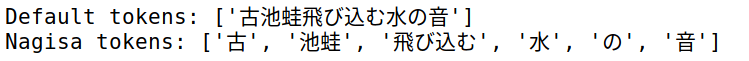
\includegraphics[width=\linewidth]{{ch_dtm/haiku.py}.png}
  \end{tcolorbox}%
  \begin{tcolorbox}[title=R Output]
      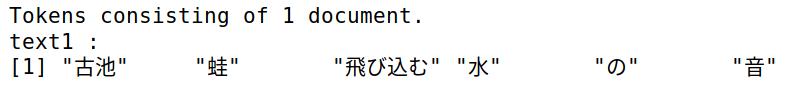
\includegraphics[width=\linewidth]{{ch_dtm/haiku.r}.png}
  \end{tcolorbox}%
\end{tcbraster}
  \caption{Tokenization of Japanese verse}\label{ex:haiku}
\end{ccsexample}



Note that for languages such as Chinese, Japanese, and Korean, which do not use spaces to delimit words, the story is more difficult.
Although a full treatment is beyond the scope of this book, \refex{haiku} shows a small example of tokenizing Japanese text,
in this case the famous haiku ``the sound of water'' by Bash\={o}.
The default tokenizer in quanteda actually does a good job, in contrast to the default python tokenizer
that simply keeps the whole string as one word
(which makes sense since this tokenizer only looks for whitespace or punctuation).
For python the best bet is to use a custom package for tokenizing Japanese, such as the \pkg{nagisa} package.
This package contains a tokenizer which is able to tokenize the Japanese text, and we could use this in the \cls{CountVectorizer}
much like we used the \cls{TreebankWordTokenizer} for English earlier.
Similarly, with heavily inflected languages such as Hungarian or Arabic,
it might be better to use preprocessing tools developed specifically for these languages, but treating those is unfortunately
beyond the scope of this book. 


\subsection{The DTM as a Sparse Matrix}

\pyrex[caption=Example document-term matrix]{ch_dtm/sotu}

\refex{sotu} shows a more realistic example.
It downloads all US 'State of the Union' speeches and creates a document-term matrix from them.
Since the matrix is now easily too large to print, both python and R simply list the size of the matrix.
R lists $85$ documents (rows) and $17,999$ features (columns), and Python reports that it's size is $85\times22219$.
Note the difference in the amount of columns (unique terms) due to the differences in tokenization as discussed above. 

\pyrex[caption=A look inside the DTM]{ch_dtm/freq}
\pyrex[caption=A look inside the DTM]{ch_dtm/freq2}

In \refex{freq} we show how you can look at the contents of the DTM. First, we show the overall term and document frequencies of each word, where we showcase words at different frequencies. Unsurprisingly, the word \emph{the} tops both charts, but further down there are minor differences.
In all cases, the highly frequent words are mostly functional words like \emph{them} or \emph{first}. More informative words such as \emph{investments} are by their nature used much less often.
Such term statistics are very useful to check for noise in the data and get a feeling of the kind of language that is used. 
Second, we take a look at the frequency of these same words in four speeches from Truman to Obama. All use words like \emph{the} and \emph{first}, but none of them talk about \emph{defrauded} -- which is not surprising, since it was only used once in all the speeches in the corpus.

However, the words that ranked around 1,000 in the top frequency are still used in less than half of the documents.
Since there are about 17,000 even less frequent words in the corpus, you can imagine that most of the document-term matrix consists of zeroes. 
The output also noted this \concept{sparsity} in the first output above.
In fact, R reports that the dtm is $91\%$ sparse, meaning that percentage of all entries is zero.
Python reports a similar figure, namely that there are only just under 150 thousand non-zero entries
out of a possible $8\times22219$, which boils down to a 92\% sparse matrix.

Note that to display the matrix we turned it from a \concept{sparse matrix} representation into a \concept{dense matrix}.
Briefly put, in a dense matrix, all entries are stored as a long list of numbers, including all the zeroes.
In a sparse matrix,  only the non-zero entries and their location are stored. 
This conversion (using the function \verb|as.matrix| and \verb|todense| respectively), however, was only performed after selecting a small subset of the data.
In general,  it is very inefficient to store and work with the matrix in a \concept[dense matrix]{dense} format.
For a reasonably large corpus with tens of thousands of documents and different words, this can quickly run billions of numbers,
which can cause problems even on modern computers and is moreover very inefficient.
With sparsities of often above 99\%, using a sparse matrix representation can easily reduce storage requirements by a hundred times and in the process speed up calculations by reducing the number of entries that need to be inspected.
Both \quanteda\ and \sklearn\ store DTMs as sparse matrices by default,
and most analysis tools are able to deal with sparse matrices very efficiently.
(but see \refsec{workflow} for problems with machine learning on sparse matrices in R). 

A final note on the difference between python and R in this example.
The code in R is much simpler and produces nicer results since it also shows the words and the speech names.
In python, we wrote our own helper function to create the frequency statistics which is built into the R \quanteda\ package.
These differences between Python and R reflect a pattern that is true in many (but not all) cases:
In python libraries such as \numpy\ and \sklearn\ are setup to maximize performance,
while in R a library such as \quanteda\ or \tidyverse\ is more geared towards ease of use.
For that reason, the DTM in python does not `remember' the actual words, it uses the index of each word,
so it consumes less memory if you don't need to use the actual words in e.g. a machine learning setup.
R, on the other hand, stores the words and also the document IDs and metadata in the DFM object.
This is easier to use if you need to look up a word or document, but it consumes (slightly) more memory. 


\begin{feature}
  \textbf{R: Why is it a document-feature matrix?}
The package \pkg{quanteda} uses the term document-feature matrix because the columns can also contain
other information instead of terms, such as word pairs, and these are collectively called \emph{features} of the text.
\end{feature}

\begin{feature}
\noindent\textbf{Python: Why fit\_transform?}
In Python, you don't have a function that directly transforms text into a DTM.
Instead, you create an \emph{transformer} called a CountVectorizer,
which can then be used to 'vectorize' texts (turn it into a row of numbers)
by counting how often each word occurs.
This uses the \fn{fit\_transform} function which is offered by all \sklearn\ transformers.
It `fits' the model on the training data, which in this case means learning the vocabulary.
It can then be used to transform other data into a DTM with the exact same columns,
which is often required for algorithms.
Because the feature names (the words themselves) are stored in the CountVectorizer
rather than the document-term matrix, you generally need to keep both objects.
\end{feature}

\subsection{The DTM as a `bag of words'}


As you can see already in these simple examples, the document-term matrix discards quite a lot of information from text.
Specifically, it disregards the order or words in a text: `John fired Mary' and `Mary fired John' both result in the same DTM,
even though the meaning of the sentences is quite different.
For this reason, a DTM is often called a \concept{bag of words}, in the sense that all words in the document are simply put in a big bag
without looking at the sentences or context of these words. 

Thus, the DTM can be said to be a specific and `lossy' representation of the text, that turns out to be quite useful for certain tasks:
The frequent occurrence of words like ``employment'', ``great'', or ``I'' might well be good indicators that a text is about the economy,
is positive, or contains personal expressions respectively.
As we will see in the next chapter, the DTM representation can be used for many different text analyses, from dictionaries to supervised and unsupervised machine learning.

Sometimes, however, you need information that is encoded in the order of words.
For example, in analysing conflict coverage it might be quite important to know who attacks whom, not just that attacking took place.
In the last section of this chapter we will look at some ways to create a richer matrix-representation by using word pairs.
Although it is beyond the scope of this book,
you can also use automatic syntactic analysis to take grammatical relations into account as well.
As is always the case with automatic analyses, it is important to understand what information the computer is looking at,
as the computer cannot find patterns in information that it doesn't have.

\subsection{The (unavoidable) Word Cloud}

One of the most famous text visualizations is without doubt the word cloud.
Essentially, a word cloud is an image where each word is displayed in a size that is representative of its frequency.
Depending on preference, word position and colour can be random, depending on word frequency, or in a decorative shape.

Word Clouds are often criticised since they are (sometimes) pretty but mostly not very informational.
The core reason for that is that only a single aspect of the words is visualized (frequency),
and simple word frequency is often not that informative: the most frequent words are generally uninformative `stop words' like ``the'' and ``I''.

For example, \refex{wordcloud} shows the word cloud for the state of the union speeches downloaded above.
In R, this is done using the \quanteda\ function \fn{textplot\_wordcloud}.
In Python we need to work a little harder, since it only has the counts, not the actual words.
So, we sum the DTM columns to get the frequency of each word, and combine that with the feature names (words)
from the |CountVectorized| object |cv|. Then we can create the WordCloud and give it the frequencies to use.
Finally, we plot the cloud and remove the axes.

\pyrex[caption=Word Cloud of the US State of the Union corpus,format=png]{ch_dtm/wordcloud}

The results from Python and R look different at first -- for one thing, R is nice and round but Python has more colors!
However, if you look at the cloud you can see both are not very meaningful: the largest words are all punctuation or words like
`a', `and', or `the'.
You have to look closely to find words like `federal' or `security' that give a hint on what the texts were actually about.



\section{Weighting and selecting documents and terms}
\label{sec:dtmselect}

\subsection{Stopword removal}

\subsection{Trimming a DTM}


\subsection{Weighting a DTM}


\section{Advanced representation of text}
\label{ngram}

The examples above all created document-term matrices where each column actually represents a word.
There is more information in a text, however, than pure word counts.
The phrases: \emph{the movie was not good, it was in fact quite bad} and \emph{the movie was not bad, in fact it was quite good}
have exactly the same word frequencies, but are quite different in meaning.
Similarly, \emph{the new residents of York} and \emph{the residents of New York} are talking about quite different people. 

Of course, in the end which aspect of the meaning of a text is important depends on your research question:
if you want to know the sentiment about the movie, it is important to take a word like `not' into account;
but if you are interested in the topic or genre of the review, or the extremity of the language used, this might not be relevant.

The core idea of this section is that in many cases this information can be captured in a DTM by having the columns represent different information than just words, for example word combinations or groups of related words.
This is often called \concept{feature engineering}, as we are using our domain expertise to find the right features (columns, independent variables) to capture the relevant meaning for our research question.
If we are using other columns than words it is also technically more correct to use the name \concept{Document-feature matrix}, as \quanteda\ does, but we will stick to the most common name here and simply continue using the name DTM.

\subsection{N-grams}

The first feature we will discuss are n-grams.
The simplest case is a bigram (or 2-gram), where each feature is a pair of adjacent words.
The example used above, \emph{the movie was not bad}, will yield the following bigrams: \emph{the-movie}, \emph{movie-was}, \emph{was-not}, and \emph{not-bad}.
Each of those bigrams is then treated as a feature, that is, a DTM would contain one column for each word pair.

As you can see in this example, we can now see the difference between \emph{not-bad} and \emph{not-good}.
The downside of using n-grams is that there are many more unique word pairs than unique words,
so the resulting DTM will have many more columns.
Moreover, there is a bigger \concept{data scarcity problem}, as each of those pairs will be less frequent,
making it more difficult to find sufficient examples of each to generalize over.

Although bigrams are the most frequent use case, trigrams (3-grams) and (rarely) higher-order n-grams can also be used.
As you can imagine, this will create even bigger DTMs and worse data scarcity problems,
so require even more attention paid to feature selection and/or trimming.


\pyrex[caption=Generating n-grams]{ch_dtm/ngram}

\refex{ngram} shows how n-grams can be created and used in Python and R.
In Python, you can pass the \verb|ngram=(n, m)| option to the vectorizer,
while R has a \verb|tokens_ngrams(n:m)| function.
Both will post-process the tokens to create all n-grams in the range of n to m.
In this example, we are asking for unigrams (i.e., the words themselves), bigrams and trigrams of a simple example sentence.
Both languages produce the same output, with R separating the words with an underscore while python uses a simple space.

\pyrex[caption=Words and bigrams containing 'government',output=r,format=table]{ch_dtm/ngram2}

\refex{ngram2} shows how you can generate n-grams for a whole corpus.
In this case, we create a DTM of the state of the union matrix with all bigrams included.
A glance at the frequency table for all words containing \emph{government} shows that,
besides the word itself and it's plural and possessive forms, the bigrams include compound words (federal and local government),
phrases with  the government as subject (the government can and must), and nouns for which the government is an adjective
(government spending and government programs).

You can imagine that including all these words as features will add many possibilities for analysis of the DTM
which would not be possible in a normal bag-of-words approach.
The terms local and federal government can be quite important to understand policy positions,
but for e.g. sentiment analysis a bigram like \emph{not good} would also be insightful
(but make sure 'not' is not on your stop word list!).   

\subsection{Collocations}

A special case of n-grams are collocations.
In the strict corpus linguistic sense of the word, collocations are pairs of words that occur more frequently than expected
based on their underlying occurence.
For example, the phrase \emph{crystal clear} presumably occurs much more often than would be expected by chance given
how often \emph{crystal} and \emph{clear} occur separately.
Collocations are important for text analysis since they often have a specific meaning,
for example because they refer to names such as \emph{New York} or disambiguate a term like \emph{sound} in \emph{sound asleep},
a \emph{sound proposal}, or \emph{loud sound}.

\refex{colloc} shows how to identify the most `surprising' collocations using R and Python.
For Python, we use the \pkg{gensim} package which we will also use for topic modeling in \refsec{unsupervised}.
This package has a \cls{Phrases} class which can identify the bigrams in a list of tokens.
In R, we use the \fn{textstat\_collocations} function from \quanteda.
These packages each use a different implementation: \pkg{gensim} uses pointwise mutual information, i.e.
how much information about finding the second word does seeing the first word give you?
Quanteda estimates an interaction parameter in a loglinear model.
Nonetheless, both methods give very similar results, with Saddam Hussein, the Iron Curtain, Al Qaida, and red tape topping the list for each.


\begin{ccsexample}
\doublecodex{ch_dtm/colloc}
\codexoutputtable{ch_dtm/colloc.r}
\doublecodex{ch_dtm/colloc2}
\codexoutputtable{ch_dtm/colloc2.r}
\caption{Identifying and applying collocations in the US State of the Union}\label{ex:colloc}
\end{ccsexample}


The next block demonstrates how to use these collocations in further processing.
In R, we filter the collocations list on $lambda>8$ and use the \fn{tokens\_compound} function to compound bigrams from that list.
As you can see in the term frequencies filtered on `hussein', the regular terms (apart from the posessive) are removed and the compounded term now has 26 occurrences.
For Python, we use the \cls{PhraseTransformer} class, which is an adaptation of the \cls{Phrases} class to the \sklearn\ methodology.
After setting a standard threshold of 0.7, we can use \fn{fit\_transform} to change the tokens.
The term statistics again show how the individual terms are now replaced by their compound. 


\subsection{Word Embeddings}

A recent addition to the text analysis toolbox are \concept{word embeddings}.
Although it is beyond the scope of this book to give a full explanation of the algorithms behind word embeddings,
they are relatively easy to understand and use at an intuitive level.

The first core idea behind word embeddings is that the meaning of a word can be expressed using a relatively small \concept{embedding vector}, generally consisting of around 300 numbers which can be interpreted as dimensions of meaning.
The second core idea is that these embedding vectors can be derived by scanning the context of each word in millions and millions of documents.


These embedding vectors can then be used as features or DTM columns for further analysis.
Using embedding vectors instead of word frequencies has the advantages of strongly reducing the dimensionality of the DTM:
instead of (tens of) thousands of columns for each unique word we only need hundreds of columns for the embedding vectors.
This means that further processing can be more efficient as fewer parameters need to be fit,
or conversely that more complicated models can be used without blowing up the parameter space.
Another advantage is that a model can also give a result for words it never saw before, as these words most likely will have an embedding vector and so can be fed into the model.
Finally, since words with similar meanings should have similar vectors,
a model fit on embedding vectors gets a `head start' since the vectors for words like `great' and `fantastic' will already be relatively close to each other, while all columns in a normal DTM are treated independently.

\newcommand{\fnglove}{\footnote{The full embedding models can be downloaded from https://nlp.stanford.edu/projects/glove/. To make the file easier to download, we took only the 10,000 most frequent words of the smallest embeddings file (the 50 dimension version of the 6B tokens model). For serious applications you probably want to download the larger files, in our experience the 300 dimension version usually gives good results. Note that the files on that site are in a slightly different format which lacks the initial header line, so if you want to use other vectors for the examples here you can convert them with the \fn{glove2word2vec} function in the \pkg{gensim} package. For R, you can also simply omit the \verb|skip=1| argument as apart from the header line the formats are identical}}

The assumption that words with similar meanings have similar vectors can also be used directly to extract synonyms.
This can be very useful, for example for (semi-)automatically expanding a dictionary for a concept.
\refex{embedding} shows how to download and use pre-trained embedding vectors to extract synonyms.
First, we download a very small subset of the pre-trained Glove embedding vectors\fnglove,
wrapping the download call in a condition to only download it when needed.

Then, for Python, we use the excellent support from the \pkg{gensim} package to load the embeddings into a \cls{KeyedVectors} object.
Although not needed for the rest of the example, we create a pandas DataFrame from the internal embedding values so the internal structure becomes clear: each row is a word, and the columns (in this case 50) are the different (semantic) dimensions that characterize that word according to the embeddings model.
This data frame is sorted on the first dimension, which shows that negative values on that dimension are related to various sports.
Next, we switch back to the \cls{KeyedVectors} object to get the most similar words to the word \emph{fraud}, which is apparently related to similar words like \emph{bribery} and \emph{corruption} but also to words like \emph{charges} and \emph{alleged}.
These similarities are a good way to (semi-)automatically expand a dictionary: start from a small list of words,
find all words that are similar to those words, and if needed manually curate that list.
Finally, we use the embeddings to solve the `analogies' that famously showcase the geometric nature of these vectors:
if you take the vector for \emph{king}, subtract the vector for \emph{man} and add that for \emph{woman},
the closest word to the resulting vector is \emph{queen}.
Amusingly, it turns out that soccer is a female form of football, probably showing the American cultural origin of the source material.

For R, there was less support from existing packages so we decided to use the opportunity to show both the conceptual simplicity of embeddings vectors and the power of matrix manipulation in R.
Thus, we directly read in the word vector file which has a head line and then on each line a word followed by its 50 values.
This is converted to a matrix with the rownames showing the word,
which we normalize to (Euclidean) length of one for each vector for easier processing. 
To determine similarity, we take the cosine distance between the vector representing a word with all other words in the matrix.
As you might remember from algebra, the cosine distance is the dot product between the vectors normalized to have length one
(just like Pearson's product-moment correlation is the dot product between the vectors normalized to z-scores per dimension).
Thus, we can simply multiply the normalized target vector with the normalized matrix to get the similarity scores.
These are then sorted, renamed, and the top values are taken using the basic functions from \refchap{datawrangling}.
Finally, analogies are solved by simply adding and subtracting the vectors as explained above, and then listing the closest words to the resulting vector
(excluding the words in the analogy itself). 

\begin{ccsexample}
\doublecodex{ch_dtm/embeddings0}
\doublecodex{ch_dtm/embeddings1}
\codexoutputtable{ch_dtm/embeddings1.r}
\doublecodex{ch_dtm/embeddings2}
\codexoutputtable{ch_dtm/embeddings2.r}
\doublecodex{ch_dtm/embeddings3}
\codex[caption=Output]{ch_dtm/embeddings3.r.out}
\caption{Using word embeddings for finding similar and analogous words}\label{ex:embedding}
\end{ccsexample}





\subsection{Linguistic Preprocessing}
\label{sec:nlp}

A final technique to be discussed here is the use of linguistic preprocessing steps to enrich and filter a DTM.
So far, all techniques discussed here are language independent.
However, there are also many language-specific tools for automatically enriching text developed by computational linguistics communities around the world.
Two techniques will be discussed here as they are relatively widely available for many languages and easy and quick to apply: \concept{Part-of-speech tagging} and \concept{lemmatizing}.

In \concept{part-of-speech tagging} or POS-tagging, each word is enriched with information on its function in the sentence: verb, noun, determiner etc.
For most languages, this can be determined with very high accuracy, although sometimes text can be ambiguous:
in one famous example, the flies in \emph{fruit flies} is generally a noun (fruit flies are a type of fly), but it can also be a verb (if fruit could fly). 
Although there are different sets of POS tags used by different tools, there is broad agreement on the core set of tags listed in \reftab{postags}.

%TODO: Add tabel with pos tags and reference to jurafsky

POS tags are useful since they allow us for example to analyse only the \textit{nouns} if we care about the things that are discussed, only the \textit{verbs} if we care about actions that are described, or only the \textit{adjectives} if we care about the characteristics given to a noun.
Moreover, knowing the POS tag of a word can help disambiguate it.
For example, like as a verb (I like books) is generally positive, but like as a preposition (a day like no other) has no clear sentiment attached.

\concept{Lemmatizing} is a technique for reducing each word to its root or \concept{lemma} (plural: lemmata).
For example, the lemma of the verb \emph{reads} is (to) \emph{read} and the lemma of the noun \emph{books} is \emph{book}.
Lemmatizing is useful since for most of our research question we do not care about these different conjugations of the same word.
By lemmatizing the texts, we do not need to include all conjugations in a dictionary,
and it reduces the dimensionality of the DTM -- and thus also the data scarcity.

Note that lemmatizing is related to a technique called \emph{stemming}, which removes known suffixes (endings) from words.
For example, for English it will remove the `s' from both reads and books.
Stemming is much less sophisticated than lemmatizing, however, and will trip over irregular conjugations
(e.g. \emph{are} as a form of to be) and regular word endings that look like conjugations (e.g. \emph{virus} will be stemmed to \emph{viru}).
English has relatively simple conjugations and stemming can produce adequate results.
For morphologically richer languages such as German or French, however, it is strongly advised to use lemmatizing instead of stemming.
Even for English we would generally advise lemmatization since it is so easy nowadays and will yield better results than stemming.

For \refex{udpipe}, we use the \concept{UDPipe} natural language processing toolkit \citep{udpipe},
a `Pipeline' that parses text into `Universal Dependencies', a representation of the syntactic structure of the text.
For R, we can immediately call the \fn{udpipe} function from the package of the same name.
This parses the given text and returns the result as a data frame with one token (word) per row,
and the various features in the columns.
For Python, we need to take some more steps ourselves.
First, we download the English models if they aren't present.
Second, we load the model and create a pipeline with all default settings,
and use that to parse the same sentence.
Finally, we use the \pkg{conllu} package to read the results into a form that can be turned into a data frame.

In both cases, the resulting tokens clearly show some of the potential advantages of lingusitic processing:
The lemma column shows that it correctly deals with irregular verbs and plural forms.
Looking at the upos (universal Part-of-Speech) column, John is recognized as a proper name (PROPN), brought as a verb, and knives as a noun.
Finally, the \verb|head_token_id| and \verb|dep_rel| columns represent the syntactic information in the sentence:
`Bought' (token 2) is the root of the sentence, and `John' is the subject (nsubj) while `knives' is the object of the buying.

\pyrex[caption=Using UDPipe to analyse a sentence,format=table,output=r]{ch_dtm/udpipe}

The syntactic relations can be useful if you need to differentiate between who is doing something and whom it was done to.
For example, one of the authors of this book used syntactic relations to analyse conflict coverage,
where there is an important difference between attacking and getting attacked \citep{clause}.
However, in most cases you probably don't need this information and analysing dependency graphs is relatively complex.
We would advise you to almost always consider lemmatizing and tagging your texts, as lemmatizing is simply so much better than stemming
(especially for languages other than English), and the Part-of-Speech can be very useful for analysing different aspects of a text. 

If you only need the lemmatizer and tagger, you can speed up processing by setting \verb|udpipe(.., parser='none')| (R) or setting the third argument to Pipeline (the parser) to \verb|Pipeline.NONE| (Python).
\refex{nouncloud} shows how this can be used to extract only the nouns from the most recent state of the union speeches,
create a DTM with these nouns, and then visualize them as a word cloud.
As you can see, these words (such as student, hero, childcare, healthcare, and terrorism), are much more indicative of the topic of a text than the general words used earlier.
In the next chapter we will show how you can further analyse these data, for example by analysing usage patterns per person or over time, or using an unsupervised topic model to cluster words into topics.

\pyrex[caption=Nouns used in the most recent State of the Union addresses,format=png,output=py]{ch_dtm/nouncloud}

Please note that we use UDPipe here, but nowadays there are a number of good and relatively easy to use linguistic toolkits that can be used.
Especially \concept{Spacy} \citep{spacy} and \concept{Stanza} \citep{stanza} are also very good and flexible toolkits with support for multiple (human) languages and good integration especially with Python.
If you want to learn more about natural language processing, the book `Speech and Language Processing' by Jurafsky and Martin is a very good starting point \citep{jurafsky}, with a third edition currently being written.


\section{Which preprocessing to use?}

This chapter has shown how to create a DTM and especially introduced a number of different steps that can be used to clean and preprocess the DTM before analysis.
All of these steps are used by text analysis practitioners and in the relevant literature.
However, no study ever uses all of these steps on top of each other.
This of courses raises the question of how to know which preprocessing steps to use for your research question.

First, there are a number of things that you should (almost) always do.
If your data contains noise such as boilerplate language, HTML artefacts, etc., you should generally strip these out before proceedings.
Second, text almost always has an abundance of uninformative (stop) words and a very long tail of very rare words.
Thus, it is almost always a good idea to use a combination of stop word removal, trimming based on document frequency, and/or tf-idf weighting.
Note that when using a stop word list, you should always manually inspect and/or fine-tune the word list to make sure it matches your domain and research question.

The other steps such as n-grams, collocations, and tagging and lemmatization are more optional but can be quite important depending on the specific research.
For this (and for choosing a specific combination of trimming and weighting), it is always good to know your domain well, look at the results, and think whether you think they make sense.
Using the example given above, bigrams can make more sense for sentiment analysis (since \emph{not good} is quite different from \emph{good}),
but for analysing the topic of texts it may be less important.

Ultimately, however, many of these questions have no good theoretical answer, and the only way to find a good preprocessing `pipeline' for your research question is to try many different
options and see which works best.
This might feel like `cheating' from a social science perspective, since it is generally frowned upon to just test many different statistical models and report on what works best.
There is a difference, however, between substantive statistical modeling where you actually want to understand the mechanisms,
and technical processing steps where you just want the best possible measurement of an underlying variable (presumably to be used in a subsequent substantive model).
\citet{mousetrap} uses the analogy of the mouse trap and the human condition: in engineering you want to make the best possible mouse trap, 
while in social science we want to understand the human condition.
For the mouse trap, it is OK if it is a black box of which we don't understand how it works, as long as we are sure that it works.
For the social science model, this is not the case as it is exactly the inner workings we are interested in.

Technical (pre)processing steps such as reviewed in this chapter are primarily engineering devices:
we don't really care how something like tf-idf works, as long as it produces the best possible measurement of the variables we need for our analysis.
In other words, it is an engineering challenge, not a social science research question.
As a consequence, the key criterion by which to judge these steps is validity, not explainability.
Thus, it is fine to try out different options, as long as you validate the results properly.
If you have many different choices to evaluate against some metric such as performance on a subsequent prediction task,
using split-half or crossvalidation techinques discussed in chapter \refchap{introsml} are also relevant here to avoid biasing the evaluation.



\setcounter{chapter}{11}
\chapter{Scraping online data}
\label{chap:scraping}

\begin{abstract}{Abstract}
In this chapter, you learn how to retrieve your data from online sources. We first discuss the use of application programming interfaces, so-called APIs, which allow you to retrieve data from social media platforms, but also government data or other forms of open data, in a machine-readable format. We then discuss how to do web scraping in a narrower sense to retrieve data from websites that do not offer an API. We also discuss how to deal with authentication mechanisms, cookies, and the like, as well as ethical, legal, and practical considerations.
\end{abstract}

\keywords{web scraping, application programming interface (API), crawling, HTML parsing}


\begin{objectives}
\item Be able to use APIs for data retrieval
\item Be able to write your own web scraper
\item Assess basics of legal, ethical, and practical constraints
\end{objectives}


\newpage
\begin{feature}
  \textbf{Packages used in this chapter}\\
  This chapter uses in particular \index{httr}\emph{httr} (R) and \index{requests}\emph{requests} (Python) to retrieve data, \index{json}\emph{json} (Python) and \index{jsonlite}\emph{jsonlite} (R) to handle JSON responses, and \index{lxml}\emph{lxml} and \index{Selenium}\emph{Selenium} for web scraping.

You can install these and some additional packages (e.g., for geocoding) with the code below if needed  (see Section~\ref{sec:installing} for more details):

\doublecodex{chapter13/chapter13install}

\noindent After installing, you need to import (activate) the packages every session:

\doublecodex{chapter13/chapter13library}
\end{feature}




%\section{Using open web APIs: from twitter and guarding to open government}
\label{sec:apis}


\section{Using Web APIs: From Open Resources to Twitter}
\label{sec:apis}

Let's assume we want to retrieve data from some online service. This
could be some social media platform, but could also be a government website,
some \emph{open data} platform or initiative, or sometimes a
commercial organization that provides some online service.  Of course,
we could surf to their website, enter a search query, and somehow save
the result. This would result in a lot of impracticalities,
though. Most notably, websites are designed such that they are
perfectly readable and understandable for humans, but the cues that
are used often have no ``meaning'' for a computer program. As humans,
we have no problem understanding which parts of a web page refer to
the author of some item on a web page, what the numbers ``2006'' and
``2008'' mean, and on. But it is not trivial to think of a way to
explain to a computer program how to identify variables like
\texttt{author}, \texttt{title}, or \texttt{year} on a web page.
We will learn how to do exactly that in Section~\ref{sec:webpages}. Writing
such a \emph{parser} is often necessary, but it is also error-prone
and  a detour, as we are trying to bring some information
that has been optimized for human reading \emph{back} to a more
structured data structure.

Luckily, however, many online services  not only have web interfaces
optimized for human reading, but also offer another possibility to
access the data they provide: an API (Application Programming
Interface).
The vast amount of contemporary web APIs works like this: you send a
\emph{request} to some URL, and you get back a  JSON object. As you
learned in Section~\ref{sec:reading}, JSON is a nested data structure, very
much like a Python dictionary (and, in fact, JSON data are typically 
represented as a dictionary in Python). In other words: APIs directly
gives us machine-readable data that we can work with without any need
to develop a custom parser.

Discussing specific APIs in a book can be a bit tricky, as there is a
chance that it will be outdated: after all, the API provider may change
it at any time. We therefore decided not to include a chapter on very
specific applications such as ``How to use the Twitter API'' or similar --
given the popularity of such APIs, a quick online search will produce
enough up-to-date (and out-of-date) tutorials on these. Instead,
we discuss the generic principles of APIs that should easily translate
to  examples other than ours.


In its  simplest form, using an API is nothing other than visiting
a specific URL. The first part of the URL specifies the so-called
API endpoint: the address of the specific API you want to use. This
address is then followed by a |?| and one or more key-value pairs with an
equal sign like this: |key=value|. Multiple key-value pairs are
separated with a \texttt{\&}.

For instance, at the time of the writing of this book, Google offers
an API endpoint, |https://www.googleapis.com/books/v1/volumes|, to search for books on Google Books.
If you want to search for books about Python, you can supply a key |q| (which stands for query) with
the value ``python'' (Example~\ref{ex:googleapi1}). We do not need any specific
software for this -- we could, in fact, use a web browser as well.
Popular packages that allow us to do it programatically are \index{httr}\emph{httr}
in combination with \index{jsonlite}\emph{jsonlite} (R) and \index{requests}\emph{requests} (Python).

But how do we know which parameters (i.e., which key-value pairs) we can use?
We need to look it up in the documentation of the API we are
interested in (in this example \url{https://developers.google.com/books/docs/v1/using}).
There is no other way of knowing that the key to submit a query
is called |q|, and which other parameters can be specified.

\begin{feature}
  In our example, we used a simple value to include in the request:
  the string ``python''.  But what if we want to submit a string that
  contains, let's say, a space, or a character like |&| or |?| which,
  as we have seen, have a special meaning in the request? In these
  cases, you need to ``encode'' your URL using a mechanism called URL
  encoding or percent encoding. You may have seen this earlier: a
  space, for instance, is represented by \texttt{\%20}
\end{feature}

\pyrex[output=py,caption={Retrieving JSON data from the Google Books API. }]{chapter13/googleapi1}

The data our request returns are nested data, and hence, they do not
really ``fit'' in a tabular data frame. We could keep the data as they
are (and then, for instance, just extract the key-value pairs that we
are interested in), but -- for the sake of getting a quick overview --
let's flatten the data so that they can be represented in a data frame
(Example~\ref{ex:googleapi2}). This works quite well here, but may be more
problematic when the items have a widely varying structure. If that
is the case, we probably would want to write a loop to iterate
over the different items and extract the information we are interested in.

\begin{ccsexample}
  \doublecodex{chapter13/googleapi2}
  \codexoutputtable{chapter13/googleapi2table.r}
  \caption{Transforming the data into a data frame.}\label{ex:googleapi2}
\end{ccsexample}

You may have realized that you did not get \emph{all} results.
This protects you from accidentally downloading a huge dataset (you
may have underestimated the number of Python books available on the
market), and saves the provider of the API a lot of bandwith.
This does not mean that you cannot get more data. In fact, many APIs work
with \emph{pagination}: you first get the first ``page'' of results,
then the next, and so on. Sometimes, the API response contains
a specific key-value pair (sometimes called a ``continuation key'')
that you can use to get the next results; sometimes, you can just
say at which result you want to start (say, result number 11) and
then get the next ``page''. You can then write a loop to retrieve
as many results as you need (Example~\ref{ex:googleapi3}) -- just make sure
that you do not get stuck in an eternal loop. When you start playing
around with APIs, make sure you do not cause unnecessary traffic,
but limit the number of calls that are made (see also Section~\ref{sec:ethicallegalpractical}).


\begin{ccsexample}
  \doublecodex{chapter13/googleapi3}
  \codexoutputtable{chapter13/googleapi3table.r}
  \caption{Full script including pagination.}\label{ex:googleapi3}
\end{ccsexample}



Many APIs work very much like the example we discussed, and you
can adapt the logic above to many APIs once you have read their
documentation. You would usually start by playing around with
single requests, and then try to automate the process by means
of a loop.

However, many APIs have restrictions regarding who can use them,
how many requests can be made, and so on.
For instance, you may need to limit the number of requests per minute
by calling a \index{sleep}\texttt{sleep} function within your loop to delay the
execution of the next call. Or, you may need to authenticate
yourself. In the example of the Google Books API, this will
allow you to request more data (such as whether you own an
(electronic) copy of the books you retrieved). In this case,
the documentation outlines that you can simply pass an authentication
token as a parameter with the URL. However, many APIs use
more advanced authentication methods such as OAuth (see Section~\ref{sec:authentication}).

Lastly, for many APIs that are very popular with social
scientists, specific wrapper packages exist (such as, to name just one example, \index{tweepy}\emph{tweepy})
which are a bit more user-friendly and handle things like authentication,
respecting rate-limits, etc., for you.


%\section{Retrieving and parsing web pages}
\label{sec:webpages}

Unfortunately, not all online services we may be interested in offer
an API -- in fact, it has even been suggested that computational
researchers has arrived in an ``post-API age'' \citep{Freelon2018}, as
API access for researchers has become increasingly restricted.

If data cannot be collected using an API (or a similar service, such
as RSS feeds), we need to resort to web scraping. Before you start a
web scraping project, make sure to ask the appropriate instances for
ethical and legal advice (see also \refsec{ethicallegalpractical}).

Web scraping (sometimes also referred to as harvesting), in essence,
boils down to automatically downloading web pages aimed at a human
audience, and extracting meaningful information out of them. One could
also say that we are reverse-engineering the way the information was
published on the web. For instance, a news site may always use a
specific formatting to denote the title of an article -- and we would
then use this to extract the title. This process is called `parsing',
which in this context is just a fancy term for `extracting meaningful
information'.

When scraping data from the web, we can distinguish two different
tasks: (1) downloading a (possibly large) number of webpages, and (2)
parsing the content of the webpages. Often, both go hand in
hand. For instance, the URL of the next page to be downloaded might
actually be parsed from the content of the current page; or some
overview page may contain the links and thus has to be parsed first in
order to download subsequent pages.

We will first discuss how to parse a single HTML page (say, the page
containing one specific product review, or one specific news article),
and then describe how to ``scale up'' and repeat the process in a
loop (to scrape, let's say, all reviews for the product; or all
articles in a specific time frame).




\subsection{Retrieving and parsing a HTML page}
\label{sec:parsehtml}
In order to parse a HTML file, you need to have a basic understanding
of the structure of an HTML file. Open your web browser, visit a
website of your choice (we suggest to use a simple page, such as
\url{http://css-book.net/d/restaurants/index.html}), and
look inspect its underlying HTML code (almost all browsers have a
function called something like ``view source'', which enables you to
do so).

You will see that there are some regular patterns in there. For
example, you may see that each paragraph is enclosed with the tags
|<p>| and |</p>|. Thinking back of \refsec{regular}, you may figure
that you could, for instance, use a regular expression to extract
the text of the first paragraph. In fact, packages like \pkg{beautifulsoup}
under the hood use regular expressions to do exactly that.

But writing your own set of regular expressions to parse a HTML
page usually is not a good idea (but it can be a last resort when
everything else fails). Chances are high that you make
a mistake or do not handle some edge case correctly; and besides,
it would be a bit like re-inventing the wheel. Packages like
\pkg{rvest} (R), \pkg{beautifulsoup}, and \pkg{lxml} (both Python)
already do this for you.

In order to use them, though, you need need to have a basic
understanding of how a HTML page looks like. Here is a simplified
example:

\begin{lstlisting}
<html>
<body>
<h1>This is a title</h1>
<div id="main">
<p> Some text with one <a href="test.html">link </a> </p>
<img src = "plaatje.jpg">an image </img>
</div>
<div id="body">
<p class="lead"> Some more text </p>
<p> Even more... </p>
<p> And more. </p>
</div>
</body>
</html>
\end{lstlisting}

For now, it is not too important to understand the function of each
specific tag (although it might help, for instance, to realize that
\texttt{a} denotes a link, \texttt{h1} a first-level heading,
\texttt{p} a paragraph and \texttt{div} some kind of section).

What is important, though, is to realize that each tag is opened and
closed (e.g. \ttt{<p>} is closed by \ttt{</p>}).
Because tags can be nested, we can actually
draw the code as a tree. In our example, this would look like this:

\dirtree{%
.1 html.
.2 body.
.3 h1.
.3 div\#main.
.4 p.
.5 a.
.4 img.
.3 div.
.4 p.lead.
.4 p.
.4 p.
}


Additionally, tags can have \emph{attributes}. For instance, the
makers of a page with customer reviews may use attributes to specify
what a section contains. For instance, they may write
\texttt{<p class="lead"> ... </div>}  to mark the lead paragraph of an article,
and \texttt{<a href=test.html"> ...</a>} specifies the target of a hyperlink.
Especially important here are the \ttt{id} and \ttt{class} attributes,
which are often used by webpages to control the formatting.
\ttt{id} (indicated with the hash sign \ttt{\#} above) gives a unique ID to a single element,
while \ttt{class} (indicated with a period) assigns a class label to one or more elements.
This enables web sites to speficy their layout and formatting using a technique called Cascading Style Sheets (CSS).
For example, the web page could set the lead paragraph to be bold.
The nice thing is that we can exploit
this information to tell our parser where to find the elements we
are interested in.



\begin{table}
  \caption{\label{tab:cssselect}Overview of CSSSelect and XPath syntax}{
  \begin{tabularx}{\textwidth}{llll}
\toprule
\multicolumn{2}{l}{Example}      & CSS Select   & XPath    \\
\midrule
\multicolumn{3}{l}{\textit{Basic tree navigation}} \\
& \ttt{h1} anywhere in document & \ttt{h1} & \ttt{//h1} \\
& \ttt{h1} inside a body & \ttt{body h1} & \ttt{//body//h1} \\
& \ttt{h1} directly inside \ttt{div} & \ttt{div > h1} & \ttt{//div/h1} \\
& Any node directly inside \ttt{div} & \ttt{div} > * & \ttt{//div/*} \\
& \ttt{p} next to a \ttt{h1} & \ttt{h1 ~ p} & \ttt{//h1/following-sibling::p} \\
& \ttt{p} next to a \ttt{h1} & \ttt{h1 + p} & \ttt{//h1/following-sibling::p[1]} \\
\multicolumn{3}{l}{\textit{Node attributes}} \\
& \ttt{<div id='x1'>} & \ttt{div\#x1} & \ttt{//div[@id='x1']} \\
& any node with \ttt{id x1} & \ttt{\#x1} & \ttt{//*[@id='x1']} \\
& \ttt{<div class='row'>} & \ttt{div.row} & \ttt{//div[@class='row']} \\
& any node with \ttt{class row} & \ttt{.row} & \ttt{//*[@class='row']} \\
& \ttt{a} with \ttt{href="\#"} & (not possible) & \ttt{//a[@href="\#"]} \\
\multicolumn{3}{l}{\textit{Advanced tree navigation}} \\
& \ttt{a} in a \ttt{div} with class 'meta' & \ttt{\#main > div.meta a} & \ttt{//*[@id='main']} \\
& $\;\;\;\;$ directly inside the \ttt{main} element & &$\;\;\;\;$ \ttt{/div[@class='meta']//a} \\
& First \ttt{p} in a \ttt{div} & \ttt{div p:first-of-type} & \ttt{//div/p[1]} \\
& First child of a \ttt{div} & \ttt{div :first-child} & \ttt{//div/*[1]} \\
& Second \ttt{p} in a \ttt{div} & \ttt{div p:nth-of-type(2)} & \ttt{//div/p[2]} \\
& Second \ttt{p} in a \ttt{div} & \ttt{div p:nth-of-type(2)} & \ttt{//div/p[2]} \\
& parent of the \ttt{div} with id \ttt{x1} & (not possible) & \ttt{//div[@id='x1']/parent::*} \\
\bottomrule
  \end{tabularx}}{}
  \end{table}


\paragraph{CSS Selectors} The easiest way to specify our parser to look for a specific element is to use a \concept{CSS Selector},
which might be familiar to you if you have created web pages.
For example, to find the lead paragraph(s) we specify \ttt{p.lead}.
To find the node with \ttt{id="body"}, we can specify \ttt{\#body}.
You can also use this to specify relations between nodes. For example,
to find all paragraphs withing the body element we would write \ttt{\#body p}.

\reftab{cssselect} gives an overview of the possibilities of CSS Select.
In general, a CSS selector is a set of node specifiers (like \ttt{h1}, \ttt{.lead} or \ttt{div\#body}),
optionally with relation specifiers between them.
So, \ttt{\#body p} finds a \ttt{p} anywhere inside the \ttt{id=body} element,
while \ttt{\#body > p} requires the \ttt{p} to be directly contained inside the body
(with no other nodes in between).

\paragraph{XPath}
An alternative to CSS Selectors is \concept{XPath}.
Where CSS Selectors are directly based on HTML and CSS styling,
XPath is a general way to describe nodes in XML (and HTML) documents.
The general form of XPath is similar to CSS Select:
a sequence of node descriptors (such as \ttt{h1} or \ttt{*[@id='body']}).
Contrary to CSS Select, you always have to specify the relationship, where
\ttt{//} means any direct or indirect descendant and \ttt{/} means a direct child.
If the relationship is not a child or decendant relationship (but for example a sibling or parent),
you specify the \concept[XPath axis]{axis} with e.g. \ttt{//a/parent::p} meaning an \ttt{a} anywhere in the document (\ttt{//a}) which has a direct parent (\ttt{/parent::}) that is a \ttt{p}. 

A second difference with CSS Selectors is that the \emph{class} and \emph{id} attributes are not given special treatment,
but can be used with the general \ttt{[@attribute='value']} pattern.
Thus, to get the lead paragraph you would specify \ttt{//p[@class='lead']}.
The big advantage of this is that you can specify any attribute (including e.g. \ttt{href=} or \ttt{data=}),
while in CSS Selectors you only have access to the \emph{class} and \emph{id}. 

The advantage of XPath is that it is a very powerful tool. 
Everything that you can describe with a CSS Selector can also be described with an XPath pattern,
but there are some thing that CSS Selectors cannot describe,
such as parents and attributes other thatn class and id.
On the other hand, CSS Selectors can be a bit harder to write, read, and debug.
You can chooose to use either tool, and you can even mix and match them in a single script,
but our general recommendation is to use CSS Selectors unless you need to use the specific abilities of XPath. 

\refex{htmlparse1} shows how to use XPATHs and CSS selectors to parse
a HTML page. To fully understand it, open
\url{http://cssbook.net/d/restaurants/index.html} in a browser and
look at its source code (all modern browsers have a function ``View
page source'' or similar), or -- more comfortable -- right-click on an
element you are interested in (such as a restaurant name) and select
``Inspect element'' or similar. This will give you a user-friendly
view of the HTML code.

\pyrex[output=py,caption={Parsing websites using XPATHs or CSS selectors}]{chapter13/htmlparse1}


Of course, \refex{htmlparse1} only parses one possible element of interest: the restaurant names. Try to retrieve other elements as well!

\begin{feature}\textbf{Do you care about children?}
Regardless of whether you use XPATHS or CSS Selectors to specify which part of the page you are interested in, it is often the case that there are other elements within it. Depending on whether you want to also retrieve the text of these elements or not, you have to use different approaches (see \refex{htmlparse2}).
\end{feature}

\pyrex[output=py,caption={Getting the text of an HTML element versus getting the text of the element and its children}]{chapter13/htmlparse2}


Notably, you may want to parse links. In HTML, links use a specific tag, |a|. These tags have an attribute, |href|, which contains the link itself. \refex{htmlparse3} shows how, after selecting the |a| tags, we can access these attributes. 

\pyrex[output=py,caption={Parsing link texts and links}]{chapter13/htmlparse3}



\begin{feature}\textbf{Pretending to be a specific browser.}  When \pkg{lxml}, \pkg{rvest}, or your web browser download a HTML page, they send a so-called HTTP request. This request contains the URL, but also some meta-data, such as a so-called user-agent string. This string specifies the name and version of the browser. Some sites may block specific user agents (such as, for instance, the ones \pkg{lxml} or \pkg{rvest} use); and sometimes, they deliver different content for different browsers. By using a more powerful module for downloading the HTML code (such as \pkg{requests} or \pkg{httr}) before parsing it, you can specify your own user-agent string and thus pretend to be a specific browser. If you do a web search, you will quickly find long lists with popular strings. In \refex{htmlparse1useragent}, we rewrote \refex{htmlparse1} such that a custom user-agent can be specified. 
\end{feature}

\pyrex[output=py,caption={Specifying a user agent to pretend to be a
    specific browser}]{chapter13/htmlparse1useragent}




\subsection{Crawling websites}
\label{sec:crawling}

Once we have mastered parsing a single HTML page, it is time to scale
up. Only rarely are we interested in parsing a single page. In most
cases, we want to use a HTML page as a starting point, parse it,
follow a link to some other interesting page, parse it as well, and so
on. There are some dedicated frameworks for this such as \pkg{scrapy},
but in our experience, it may be more of a burden to learn that
framework than to just implement your crawler yourself.

Staying with the example of a restaurant review website, we might be
interested retrieving all restaurants from a specific city, and for
all of these restaurants, all available reviews.

Our approach, thus, could look as follows:

\begin{enumerate}
	\item Retrieve the overview page.
	\item Parse the names of the hotels and the corresponding links.
	\item Loop over all the links, retrieve the corresponding pages.
	\item On each of these pages, parse the interesting content (i.e., the reviews, ratings, and so on).
\end{enumerate}

So, what if there are multiple overview pages (or multiple pages with
reviews)? Basically, there are two possibilities: The first
possibility is to look for the link to the next page, parse it,
download the next page, and so on.  The second possibility exploits
the fact that often, URLs are very systematic: For instance, the first
page of restaurants might have a URL such as
\url{http://myreviewsite.com/amsterdam/restaurants.html?page=1}.  If this
is the case, we can simply construct a list with all possible URLs
(\refex{createurls})

\pyrex[output=py,caption={Generating a list of URLs that follow the same pattern.}]{chapter13/createurls}

Afterwards, we would just loop over this list and retrieve all the
pages (a bit like how we approached \refex{googleapi3} in \refsec{apis}).

However, often, things are not as straightforward, and we need to find
the correct links on a page that we have been parsing -- that's why we
\emph{crawl} through the website.

Writing a good crawler can take some time, and they will look very
differently for different pages. The best advice is to build them up
step-by-step. Carefully inspect the website you are interested in.
Take a sheet of paper, draw its structure, and try to find out which
pages you need to parse, and how you can get from one page to the next.
Also think about how the data that you want to extract should be organized.

We will illustrate this process using our mockup review website \url{http://cssbook.net/d/restaurants/}.
First, have a look at the site and try to understand its structure.

You will see that it has an overview page, |index.html|, with the
names of all restaurants and, per restaurant, a link to a page with reviews.
Click on these links, and note your observations, such as:
\begin{itemize}
\item the pages have different numbers of reviews;
\item each review consists of a author name, a review text, and a rating;
\item some, but not all, pages have a link saying ``Get older reviews''
\item \ldots
\end{itemize}

If you combine what you just learned about extracting text and links from HTML
pages with your knowledge about control structures like loops and conditional
statements (\refsec{controlstructures}), you can now write your own crawler.

Writing a scraper is a craft, and there are several ways of achieving your goal.
You probably want to develop your scraper in steps: first write a function to
parse the overview page, then a function to parse the review pages, then try
to combine all elements into one script. Before you read on, try to write
such a scraper.

To show you one possible solution, we implemented a scraper in Python
that crawls and parses all reviews for all restaurants
(\refex{crawling}), which we describe in detail below.

\pyrex[output=py,input=py,caption={Crawling a website}]{chapter13/crawling}

First, we need to get a list of all restaurants and the links to their
reviews. That's what is done in the function |get_restaurants|. This
is actually the first thing we do (see line 34--35).

We now want to loop over these links and retrieve the reviews.  We
decided to use a \emph{generator} (\refsec{controlstructures}): instead of writing a
function that collects \emph{all} reviews in a list first, we let the
function yield each review immediately -- and immediately append that review
to a file. This has a big advantage: if our scraper fails (for
instance, due to a time out, a block, or a programming error), then we
already saved the reviews we got so far.

We loop over the links to the restaurants (line 38) and call the
function |get_reviews| (line 40). Each review it returns (the review
is a dict) gets the name of the restaurant as an extra key, and then
gets written to a file which contains one JSON-object per line (also
known as a jsonlines-file).

The function |get_reviews| takes a link to a review page as input and
yields reviews. If we knew all pages with reviews already, then we
would not need the while loop statement in line 16 and the lines
28--33. However, as we have seen, some review pages contain a link to
older reviews. We therefore use a loop that runs forever (that is what
|while True:| does), \emph{unless} it encounters a |break| statement
(line 33).  An inspection of the HTML code shows that these links have
a |span| tag with the attribute |class="backbutton"|. We therefore
check if such a button exists (line 27), and if so, we get its |href|
attribute (i.e., the link itself), overwrite the |url| variable with
it, and then go back to line 16, the beginning of the loop, so that we
can download and parse this next URL.  This goes on as long as such a
link is not found any more.



\subsection{Dynamic web pages}
\label{sec:selenium}

You may have realized that all our scraping efforts until now
proceeded in two steps: we retrieved (downloaded) the HTML source of a
web page and then parsed it. However, modern websites more and more
are dynamic instead of static. For example, after being loaded, they
load additional content, or what is displayed changes based on what
the user does. Frequently, some JavaScript is run within the user's
browser to do that. However, we do not have a browser here. The HTML
code we downloaded may contain some instructions for the browser that
some code needs to be run, but in the absence of a browser, our Python
or R script cannot do this.

A first test to check out whether this is a concern, you can simply
check whether the HTML code in your browser is the same that you would
get if you downloaded it with R or Python.  After having retrieved the
page (\refex{htmlparse1useragent}), you simply dump it to a file
(\refex{htmltofile}) and open this file in your browser to verify that
you indeed downloaded what you intended to download (and not, for
instance, a login page, a cookie wall, or an error message).

\pyrex[output=none,caption={Dumping the HTML source to a file}]{chapter13/htmltofile}


If this test indeed shows that the data you are interested in is
indeed not part of the HTML code you can retrieve with R or Python,
use the following checklist to find

\begin{enumerate}
\item Does using a different user-agent string (see above) solve the issue?
\item Is the issue due to some cookie that needs to be accepted or you need to log in (see below)?
\item Is a different page delivered for different browsers, devices, display settings, etc.?
\end{enumerate}

If all of this does not help, or if you already know for sure that the
content you are interested in is dynamically fetched via JavaScript or
similar, you can use \pkg{selenium} to literally start a browser and
extract the content you are interested in from there. Selenium has
been designed for testing web sites and allows you to automate clicks
etc. in a browser window, and also supports CSS selectors and XPATHS
to specify parts of the web page.

Using selenium may require some additional setup on your computer,
which may depend on your operating system and software versions you
are using -- check out the usual online sources for guidance if
needed.  It is possible to use Selenium through R using
\pkg{Rselenium}. However, doing so can be quite a hassle and requires,
for instance, running a separate Selenium server, for instance using
Docker. If you opt to use Selenium for web scraping, your safest bet
is probably to follow an online tutorial and/or to dive into the
documentation. To give you a first impression of the general working,
\refex{selenium} shows you how to (at the time of writing of this
book) open Firefox, surf to Google, google for Tintin by entering that
string and pressing the Return key, click on the first link containing
that string, and take a screenshot of the result.

\pyrex[output=none,input=py,caption={Using Selemium to literally open a browser, input text, click on a link, and take a screenshot.}]{chapter13/selenium}


\begin{feature}\textbf{Loosing your head}
If you want to run long-lasting scraping processes using Selenium on
the background (or on a server without a graphical user interface),
you may want to look into what is called a ``headless'' browser. For
instance, Selenium can start Firefox in ``headless'' mode, which means
that it will run without making any connection to a graphical
interface. Of course, that also means that you cannot watch Selenium
scrape, which may make debugging more difficult. You could opt for
developing your scraper first using a normal browser, and then
changing it to use a headless browser once everything works.
\end{feature}


\section{Retrieving and Parsing Web Pages}
\label{sec:webpages}

Unfortunately, not all online services we may be interested in offer
an API -- in fact, it has even been suggested that computational
researchers have arrived in an ``post-API age'' \citep{Freelon2018}, as
API access for researchers has become increasingly restricted.

If data cannot be collected using an API (or a similar service, such
as RSS feeds), we need to resort to web scraping. Before you start a
web scraping project, make sure to ask the appropriate  authorities for
ethical and legal advice (see also Section~\ref{sec:ethicallegalpractical}).

Web scraping (sometimes also referred to as harvesting), in essence,
boils down to automatically downloading web pages aimed at a human
audience, and extracting meaningful information out of them. One could
also say that we are reverse-engineering the way the information was
published on the web. For instance, a news site may always use a
specific formatting to denote the title of an article -- and we would
then use this to extract the title. This process is called ``parsing'',
which in this context is just a fancy term for ``extracting meaningful
information''.

When scraping data from the web, we can distinguish two different
tasks: (1) downloading a (possibly large) number of webpages, and (2)
parsing the content of the webpages. Often, both go hand in
hand. For instance, the URL of the next page to be downloaded might
actually be parsed from the content of the current page; or some
overview page may contain the links and thus has to be parsed first in
order to download subsequent pages.

We will first discuss how to parse a single HTML page (say, the page
containing one specific product review, or one specific news article),
and then describe how to ``scale up'' and repeat the process in a
loop (to scrape, let's say, all reviews for the product; or all
articles in a specific time frame).




\subsection{Retrieving and Parsing an HTML Page}
\label{sec:parsehtml}
In order to parse an HTML file, you need to have a basic understanding
of the structure of an HTML file. Open your web browser, visit a
website of your choice (we suggest to use a simple page, such as
\url{http://css-book.net/d/restaurants/index.html}), and
 inspect its underlying HTML code (almost all browsers have a
function called something like ``view source'', which enables you to
do so).

You will see that there are some regular patterns in there. For
example, you may see that each paragraph is enclosed with the tags
|<p>| and |</p>|. Thinking back to Section~\ref{sec:regular}, you may figure out 
that you could, for instance, use a regular expression to extract
the text of the first paragraph. In fact, packages like \index{beautifulsoup}\emph{beautifulsoup}
under the hood use regular expressions to do exactly that.

But writing your own set of regular expressions to parse an HTML
page is usually not a good idea (but it can be a last resort when
everything else fails). Chances are high that you will make
a mistake or  not handle some edge case correctly; and besides,
it would be a bit like re-inventing the wheel. Packages like
\index{rvest}\emph{rvest} (R), \index{beautifulsoup}\emph{beautifulsoup}, and \index{lxml}\emph{lxml} (both Python)
already do this for you.

In order to use them, though, you need need to have a basic
understanding of what an HTML page looks like. Here is a simplified
example:

\begin{lstlisting}
<html>
<body>
<h1>This is a title</h1>
<div id="main">
<p> Some text with one <a href="test.html">link </a> </p>
<img src = "plaatje.jpg">an image </img>
</div>
<div id="body">
<p class="lead"> Some more text </p>
<p> Even more... </p>
<p> And more. </p>
</div>
</body>
</html>
\end{lstlisting}

For now, it is not too important to understand the function of each
specific tag (although it might help, for instance, to realize that
\texttt{a} denotes a link, \texttt{h1} a first-level heading,
\texttt{p} a paragraph and \texttt{div} some kind of section).

What is important, though, is to realize that each tag is opened and
closed (e.g., \texttt{\small{<p>}} is closed by \texttt{\small{</p>}}).
Because tags can be nested, we can actually
draw the code as a tree. In our example, this would look like this:

\dirtree{%
.1 html.
.2 body.
.3 h1.
.3 div\#main.
.4 p.
.5 a.
.4 img.
.3 div.
.4 p.lead.
.4 p.
.4 p.
}


Additionally, tags can have \emph{attributes}. For instance, the
makers of a page with customer reviews may use attributes to specify
what a section contains. For instance, they may write
\texttt{<p class="lead"> ... </div>}  to mark the lead paragraph of an article,
and \texttt{<a href=test.html"> ...</a>} specifies the target of a hyperlink.
Especially important here are the \texttt{\small{id}} and \texttt{\small{class}} attributes,
which are often used by webpages to control the formatting.
\texttt{\small{id}} (indicated with the hash sign \texttt{\small{\#}} above) gives a unique ID to a single element,
while \texttt{\small{class}} (indicated with a period) assigns a class label to one or more elements.
This enables web sites to specify their layout and formatting using a technique called Cascading Style Sheets (CSS).
For example, the web page could set the lead paragraph to be bold.
The nice thing is that we can exploit
this information to tell our parser where to find the elements we
are interested in.

%

\begin{table}
  \caption{\label{tab:cssselect}Overview of CSSSelect and XPath syntax}{
  \begin{tabularx}{\textwidth}{llll}
\toprule
\multicolumn{2}{l}{Example}      & CSS Select   & XPath    \\
\midrule
\multicolumn{3}{l}{\textit{Basic tree navigation}} \\
& \ttt{h1} anywhere in document & \ttt{h1} & \ttt{//h1} \\
& \ttt{h1} inside a body & \ttt{body h1} & \ttt{//body//h1} \\
& \ttt{h1} directly inside \ttt{div} & \ttt{div > h1} & \ttt{//div/h1} \\
& Any node directly inside \ttt{div} & \ttt{div} > * & \ttt{//div/*} \\
& \ttt{p} next to a \ttt{h1} & \ttt{h1 ~ p} & \ttt{//h1/following-sibling::p} \\
& \ttt{p} next to a \ttt{h1} & \ttt{h1 + p} & \ttt{//h1/following-sibling::p[1]} \\
\multicolumn{3}{l}{\textit{Node attributes}} \\
& \ttt{<div id='x1'>} & \ttt{div\#x1} & \ttt{//div[@id='x1']} \\
& any node with \ttt{id x1} & \ttt{\#x1} & \ttt{//*[@id='x1']} \\
& \ttt{<div class='row'>} & \ttt{div.row} & \ttt{//div[@class='row']} \\
& any node with \ttt{class row} & \ttt{.row} & \ttt{//*[@class='row']} \\
& \ttt{a} with \ttt{href="\#"} & (not possible) & \ttt{//a[@href="\#"]} \\
\multicolumn{3}{l}{\textit{Advanced tree navigation}} \\
& \ttt{a} in a \ttt{div} with class 'meta' & \ttt{\#main > div.meta a} & \ttt{//*[@id='main']} \\
& $\;\;\;\;$ directly inside the \ttt{main} element & &$\;\;\;\;$ \ttt{/div[@class='meta']//a} \\
& First \ttt{p} in a \ttt{div} & \ttt{div p:first-of-type} & \ttt{//div/p[1]} \\
& First child of a \ttt{div} & \ttt{div :first-child} & \ttt{//div/*[1]} \\
& Second \ttt{p} in a \ttt{div} & \ttt{div p:nth-of-type(2)} & \ttt{//div/p[2]} \\
& Second \ttt{p} in a \ttt{div} & \ttt{div p:nth-of-type(2)} & \ttt{//div/p[2]} \\
& parent of the \ttt{div} with id \ttt{x1} & (not possible) & \ttt{//div[@id='x1']/parent::*} \\
\bottomrule
  \end{tabularx}}{}
  \end{table}




\begin{table}
  \caption{\label{tab:cssselect}Overview of CSSSelect and XPath syntax}{
  \begin{tabularx}{\textwidth}{llll}
\toprule
\multicolumn{2}{l}{Example}      & CSS Select   & XPath    \\
\midrule
\multicolumn{3}{l}{\textit{Basic tree navigation}} \\
& \texttt{\small{h1}} anywhere in document & \texttt{\small{h1}} & \texttt{\small{//h1}} \\
& \texttt{\small{h1}} inside a body & \texttt{\small{body h1}} & \texttt{\small{//body//h1}} \\
& \texttt{\small{h1}} directly inside \texttt{\small{div}} & \texttt{\small{div > h1}} & \texttt{\small{//div/h1}} \\
& Any node directly inside \texttt{\small{div}} & \texttt{\small{div}} > * & \texttt{\small{//div/*}} \\
& \texttt{\small{p}} next to a \texttt{\small{h1}} & \texttt{\small{h1 ~ p}} & \texttt{\small{//h1/following-sibling::p}} \\
& \texttt{\small{p}} next to a \texttt{\small{h1}} & \texttt{\small{h1 + p}} & \texttt{\small{//h1/following-sibling::p[1]}} \\
\multicolumn{3}{l}{\textit{Node attributes}} \\
& \texttt{\small{<div id='x1'>}} & \texttt{\small{div\#x1}} & \texttt{\small{//div[@id='x1']}} \\
& any node with \texttt{\small{id x1}} & \texttt{\small{\#x1}} & \texttt{\small{//*[@id='x1']}} \\
& \texttt{\small{<div class='row'>}} & \texttt{\small{div.row}} & \texttt{\small{//div[@class='row']}} \\
& any node with \texttt{\small{class row}} & \texttt{\small{.row}} & \texttt{\small{//*[@class='row']}} \\
& \texttt{\small{a}} with \texttt{\small{href="\#"}} & (not possible) & \texttt{\small{//a[@href="\#"]}} \\
\multicolumn{3}{l}{\textit{Advanced tree navigation}} \\
& \texttt{\small{a}} in a \texttt{\small{div}} with class 'meta' & \texttt{\small{\#main > div.meta a}} & \texttt{\small{//*[@id='main']}} \\
& $\;\;\;\;$ directly inside the \texttt{\small{main}} element & &$\;\;\;\;$ \texttt{\small{/div[@class='meta']//a}} \\
& First \texttt{\small{p}} in a \texttt{\small{div}} & \texttt{\small{div p:first-of-type}} & \texttt{\small{//div/p[1]}} \\
& First child of a \texttt{\small{div}} & \texttt{\small{div :first-child}} & \texttt{\small{//div/*[1]}} \\
& Second \texttt{\small{p}} in a \texttt{\small{div}} & \texttt{\small{div p:nth-of-type(2)}} & \texttt{\small{//div/p[2]}} \\
& Second \texttt{\small{p}} in a \texttt{\small{div}} & \texttt{\small{div p:nth-of-type(2)}} & \texttt{\small{//div/p[2]}} \\
& parent of the \texttt{\small{div}} with id \texttt{\small{x1}} & (not possible) & \texttt{\small{//div[@id='x1']/parent::*}} \\
\bottomrule
  \end{tabularx}}{}
  \end{table}


\paragraph{CSS Selectors} The easiest way to specify our parser to look for a specific element is to use a \index{CSS Selector}\emph{CSS Selector},
which might be familiar to you if you have created web pages.
For example, to find the lead paragraph(s) we specify \texttt{\small{p.lead}}.
To find the node with \texttt{\small{id="body"}}, we can specify \texttt{\small{\#body}}.
You can also use this to specify relations between nodes. For example,
to find all paragraphs within the body element we would write \texttt{\small{\#body p}}.

Table~\ref{tab:cssselect} gives an overview of the possibilities of CSS Select.
In general, a CSS selector is a set of node specifiers (like \texttt{\small{h1}}, \texttt{\small{.lead}} or \texttt{\small{div\#body}}),
optionally with relation specifiers between them.
So, \texttt{\small{\#body p}} finds a \texttt{\small{p}} anywhere inside the \texttt{\small{id=body}} element,
while \texttt{\small{\#body > p}} requires the \texttt{\small{p}} to be directly contained inside the body
(with no other nodes in between).

\paragraph{XPath}
An alternative to CSS Selectors is \index{XPath}\emph{XPath}.
Where CSS Selectors are directly based on HTML and CSS styling,
XPath is a general way to describe nodes in XML (and HTML) documents.
The general form of XPath is similar to CSS Select:
a sequence of node descriptors (such as \texttt{\small{h1}} or \texttt{\small{*[@id='body']}}).
Contrary to CSS Select, you always have to specify the relationship, where
\texttt{\small{//}} means any direct or indirect descendant and \texttt{\small{/}} means a direct child.
If the relationship is not a child or descendant relationship (but for example a sibling or parent),
you specify the \concept[XPath axis]{axis} with e.g. \texttt{\small{//a/parent::p}} meaning an \texttt{\small{a}} anywhere in the document (\texttt{\small{//a}}) which has a direct parent (\texttt{\small{/parent::}}) that is a \texttt{\small{p}}.

A second difference with CSS Selectors is that the \emph{class} and \emph{id} attributes are not given special treatment,
but can be used with the general \texttt{\small{[@attribute='value']}} pattern.
Thus, to get the lead paragraph you would specify \texttt{\small{//p[@class='lead']}}.
The big advantage of this is that you can specify any attribute (including, e.g., \texttt{\small{href=}} or \texttt{\small{data=}}),
while in CSS Selectors you only have access to the \emph{class} and \emph{id}.

The advantage of XPath is that it is a very powerful tool.
Everything that you can describe with a CSS Selector can also be described with an XPath pattern,
but there are some things that CSS Selectors cannot describe,
such as parents and attributes other than class and id.
On the other hand, XPath patterns can be a bit harder to write, read, and debug.
You can choose to use either tool, and you can even mix and match them in a single script,
but our general recommendation is to use CSS Selectors unless you need to use the specific abilities of XPath.

Example~\ref{ex:htmlparse1} shows how to use XPATHs and CSS selectors to parse
an HTML page. To fully understand it, open
\url{http://cssbook.net/d/restaurants/index.html} in a browser and
look at its source code (all modern browsers have a function ``View
page source'' or similar), or -- more comfortable -- right-click on an
element you are interested in (such as a restaurant name) and select
``Inspect element'' or similar. This will give you a user-friendly
view of the HTML code.

\pyrex[output=py,caption={Parsing websites using XPATHs or CSS selectors}]{chapter13/htmlparse1}


Of course, Example~\ref{ex:htmlparse1} only parses one possible element of interest: the restaurant names. Try to retrieve other elements as well!

\begin{feature}\textbf{Do you care about children?}
Regardless of whether you use XPATHS or CSS Selectors to specify which part of the page you are interested in, it is often the case that there are other elements within it. Depending on whether you want to also retrieve the text of these elements or not, you have to use different approaches (see Example~\ref{ex:htmlparse2}).
\end{feature}

\pyrex[output=py,caption={Getting the text of an HTML element versus getting the text of the element and its children}]{chapter13/htmlparse2}


Notably, you may want to parse links. In HTML, links use a specific tag, |a|. These tags have an attribute, |href|, which contains the link itself. Example~\ref{ex:htmlparse3} shows how, after selecting the |a| tags, we can access these attributes.

\pyrex[output=py,caption={Parsing link texts and links}]{chapter13/htmlparse3}



\begin{feature}\textbf{Pretending to be a specific browser.}  When \index{lxml}\emph{lxml}, \index{rvest}\emph{rvest}, or your web browser download an HTML page, they send a so-called HTTP request. This request contains the URL, but also some meta-data, such as a so-called user-agent string. This string specifies the name and version of the browser. Some sites may block specific user agents (such as, for instance, the ones that \index{lxml}\emph{lxml} or \index{rvest}\emph{rvest} use); and sometimes, they deliver different content for different browsers. By using a more powerful module for downloading the HTML code (such as \index{requests}\emph{requests} or \index{httr}\emph{httr}) before parsing it, you can specify your own user-agent string and thus pretend to be a specific browser. If you do a web search, you will quickly find long lists with popular strings. In Example~\ref{ex:htmlparse1useragent}, we rewrote Example~\ref{ex:htmlparse1} such that a custom user-agent can be specified.
\end{feature}

\pyrex[output=py,caption={Specifying a user agent to pretend to be a
    specific browser}]{chapter13/htmlparse1useragent}




\subsection{Crawling Websites}
\label{sec:crawling}

Once we have mastered parsing a single HTML page, it is time to scale
up. Only rarely are we interested in parsing a single page. In most
cases, we want to use an HTML page as a starting point, parse it,
follow a link to some other interesting page, parse it as well, and so
on. There are some dedicated frameworks for this such as \index{scrapy}\emph{scrapy},
but in our experience, it may be more of a burden to learn that
framework than to just implement your crawler yourself.

Staying with the example of a restaurant review website, we might be
interested retrieving all restaurants from a specific city, and for
all of these restaurants, all available reviews.

Our approach, thus, could look as follows:

\begin{enumerate}
	\item Retrieve the overview page.
	\item Parse the names of the restaurants and the corresponding links.
	\item Loop over all the links, retrieve the corresponding pages.
	\item On each of these pages, parse the interesting content (i.e., the reviews, ratings, and so on).
\end{enumerate}

So, what if there are multiple overview pages (or multiple pages with
reviews)? Basically, there are two possibilities: the first
possibility is to look for the link to the next page, parse it,
download the next page, and so on.  The second possibility exploits
the fact that often, URLs are very systematic: for instance, the first
page of restaurants might have a URL such as
\url{http://myreviewsite.com/amsterdam/restaurants.html?page=1}.  If this
is the case, we can simply construct a list with all possible URLs
(Example~\ref{ex:createurls})

\pyrex[output=py,caption={Generating a list of URLs that follow the same pattern.}]{chapter13/createurls}

Afterwards, we would just loop over this list and retrieve all the
pages (a bit like how we approached Example~\ref{ex:googleapi3} in Section~\ref{sec:apis}).

However, often, things are not as straightforward, and we need to find
the correct links on a page that we have been parsing -- that's why we
\emph{crawl} through the website.

Writing a good crawler can take some time, and they will look very
differently for different pages. The best advice is to build them up
step-by-step. Carefully inspect the website you are interested in.
Take a sheet of paper, draw its structure, and try to find out which
pages you need to parse, and how you can get from one page to the next.
Also think about how the data that you want to extract should be organized.

We will illustrate this process using our mock-up review website \url{http://cssbook.net/d/restaurants/}.
First, have a look at the site and try to understand its structure.

You will see that it has an overview page, |index.html|, with the
names of all restaurants and, per restaurant, a link to a page with reviews.
Click on these links, and note your observations, such as:
\begin{itemize}
\item the pages have different numbers of reviews;
\item each review consists of an author name, a review text, and a rating;
\item some, but not all, pages have a link saying ``Get older reviews''
\item \ldots
\end{itemize}

If you combine what you just learned about extracting text and links from HTML
pages with your knowledge about control structures like loops and conditional
statements (Section~\ref{sec:controlstructures}), you can now write your own crawler.

Writing a scraper is a craft, and there are several ways of achieving your goal.
You probably want to develop your scraper in steps: first write a function to
parse the overview page, then a function to parse the review pages, then try
to combine all elements into one script. Before you read on, try to write
such a scraper.

To show you one possible solution, we implemented a scraper in Python
that crawls and parses all reviews for all restaurants
(Example~\ref{ex:crawling}), which we describe in detail below.

\pyrex[output=py,input=py,caption={Crawling a website}]{chapter13/crawling}

First, we need to get a list of all restaurants and the links to their
reviews. That's what is done in the function |get_restaurants|. This
is actually the first thing we do (see line 34--35).

We now want to loop over these links and retrieve the reviews.  We
decided to use a \emph{generator} (Section~\ref{sec:controlstructures}): instead of writing a
function that collects \emph{all} reviews in a list first, we let the
function yield each review immediately -- and immediately append that review
to a file. This has a big advantage: if our scraper fails (for
instance, due to a time out, a block, or a programming error), then we
have already saved the reviews we got so far.

We loop over the links to the restaurants (line 38) and call the
function |get_reviews| (line 40). Each review it returns (the review
is a  dict) gets the name of the restaurant as an extra key, and then
gets written to a file which contains one JSON-object per line (also
known as a jsonlines-file).

The function |get_reviews| takes a link to a review page as input and
yields reviews. If we knew all pages with reviews already, then we
would not need the while loop statement in line 16 and the lines
28--33. However, as we have seen, some review pages contain a link to
older reviews. We therefore use a loop that runs forever (that is what
|while True:| does), \emph{unless} it encounters a |break| statement
(line 33).  An inspection of the HTML code shows that these links have
a |span| tag with the attribute |class="backbutton"|. We therefore
check if such a button exists (line 27), and if so, we get its |href|
attribute (i.e., the link itself), overwrite the |url| variable with
it, and then go back to line 16, the beginning of the loop, so that we
can download and parse this next URL.  This goes on until such a
link is no longer found.



\subsection{Dynamic Web Pages}
\label{sec:selenium}

You may have realized that all our scraping efforts until now
proceeded in two steps: we retrieved (downloaded) the HTML source of a
web page and then parsed it. However, modern websites more and more frequently 
are dynamic rather than static. For example, after being loaded, they
load additional content, or what is displayed changes based on what
the user does. Frequently, some JavaScript is run within the user's
browser to do that. However, we do not have a browser here. The HTML
code we downloaded may contain some instructions for the browser that
some code needs to be run, but in the absence of a browser, our Python
or R script cannot do this.

As a first test to check out whether this is a concern, you can simply
check whether the HTML code in your browser is the same as that you would
get if you downloaded it with R or Python.  After having retrieved the
page (Example~\ref{ex:htmlparse1useragent}), you simply dump it to a file
(Example~\ref{ex:htmltofile}) and open this file in your browser to verify that
you indeed downloaded what you intended to download (and not, for
instance, a login page, a cookie wall, or an error message).

\pyrex[output=none,caption={Dumping the HTML source to a file}]{chapter13/htmltofile}


If this test  shows that the data you are interested in is
indeed not part of the HTML code you can retrieve with R or Python,
and use the following checklist to find

\begin{enumerate}
\item Does using a different user-agent string (see above) solve the issue?
\item Is the issue due to some cookie that needs to be accepted or you need to log in (see below)?
\item Is a different page delivered for different browsers, devices, display settings, etc.?
\end{enumerate}

If all of this does not help, or if you already know for sure that the
content you are interested in is dynamically fetched via JavaScript or
similar, you can use \index{Selenium}\emph{Selenium} to literally start a browser and
extract the content you are interested in from there. Selenium has
been designed for testing web sites and allows you to automate clicks
etc. in a browser window, and also supports CSS selectors and XPATHS
to specify parts of the web page.

Using Selenium may require some additional setup on your computer,
which may depend on your operating system and the software versions you
are using -- check out the usual online sources for guidance if
needed.  It is possible to use  Selenium through R using
\index{Rselenium}\emph{Rselenium}. However, doing so can be quite a hassle and requires,
 running a separate Selenium server, for instance,  using
Docker. If you opt to use Selenium for web scraping, your safest bet
is probably to follow an online tutorial and/or to dive into the
documentation. To give you a first impression of the general working,
Example~\ref{ex:selenium} shows you how to (at the time of writing of this
book) open Firefox, surf to Google, google for Tintin by entering that
string and pressing the return key, click on the first link containing
that string, and take a screenshot of the result.

\pyrex[output=none,input=py,caption={Using Selenium to literally open a browser, input text, click on a link, and take a screenshot.}]{chapter13/selenium}


\begin{feature}\textbf{Loosing your head}
If you want to run long-lasting scraping processes using Selenium in
the background (or on a server without a graphical user interface),
you may want to look into what is called a ``headless'' browser. For
instance, Selenium can start Firefox in ``headless'' mode, which means
that it will run without making any connection to a graphical
interface. Of course, that also means that you cannot watch Selenium
scrape, which may make debugging more difficult. You could opt for
developing your scraper first using a normal browser, and then
changing it to use a headless browser once everything works.
\end{feature}

%\section{Authentication, cookies, and sessions}
\label{sec:authentication}

\subsection{Authentication and APIs}
\label{sec:authapi}
When we introduced APIs in \refsec{apis}, we used an example of an
API where you did not need to authenticate yourself. As we have seen,
using such an API is as simple as sending an HTTP request to an
endpoint and getting a response (usually, a JSON object) back. And
indeed, there are plenty of interesting APIs (think for instance of
open governemnt APIs) that work this way.

While this has obvious advantages for you, it also has some serious
dowmsides from the perspective of the API provider as well as from
a security and privacy standpoint. The more confidential the data is,
the more likely it is that the API provider needs to know who you
are in order to determine which data you are allowed to retrieve;
and even if the data are not confidential, authentication may be
used to limit the number of requests that an individual can make
in a given time frame.

In its most simple form, you just need to provide a unique key that
identifies you as a user. For instance, \refex{textrazor} shows how
such a key can be passed along as HTTP header, essentially as
additional information next to the URL that you want to retrieve (see
also \refsec{authweb}). The example shows a call to an endpoint
of a commercial API for natural language processing to inform how
many requests we have made today.

\pyrex[output=py,input=both, caption={Passing a key as HTTP request header to authenticate at an API endpoint}]{chapter13/textrazor}

As you see, using an API that requires authentication by passing a key
as a HTTP header is hardly more complicated than using APIs that do
not require authentication such as outlined in \refsec{apis}.
However, many APIs use more complex protocols for authentication.

The most popular one is called OAuth, and it is used by many APIs
provided by major players such as Google, Facebook, Twitter, Github,
LinkedIn, etc. Here, you have a client ID and a client secret
(sometimes also called consumer key and consumer secret) and an
access token with associated access token secret. The first pair
authenticates you as a user, the second pair authenticates the
specific ``app'' (i.e., your script). Once authenticated, your
script can then interact with the API. While it is possible to
directly work with OAuth HTTP requests using \pkg{requests\_oauthlib}
(Python) or \pkg{httr} (R), chances are relatively low that you
have to do so, unless you plan on really developing your own app
or even your own API: For all popular API's, so-called wrappers,
packages that provide a simpler interface to the API, are available
on pypi and CRAN. Still, all of these require to have at least
a consumer key and a consumer secret. The access token sometimes
is generated via a web interface where you manage your account
(e.g., in the case of Twitter), or can be acquired by your script
itself, which then will redirect the user to a website in which
they are asked to authenticate the app. The nice thing about this
is that it only needs to happen once: Once your app is authenticated,
it can keep making requests.




\subsection{Authentication and webpages}
\label{sec:authweb}
In this section, we briefly discuss different approaches for dealing
with websites where you need to log on, accept something (e.g., a
so-called cookie wall), or have to otherwise authenticate yourself.
One approach can be the use of a web testing framework like Selenium
(see \refsec{selenium}): You let your script literally open a browser
and, for instance, fill in your login information.

However, sometimes that's not necessary and we can still use simpler
and more efficent webscraping without invoking a browser. As we have already
seen in \refsec{parsehtml}, when making an HTTP request, we can transmit
additional information, such as the so-called user-agent string. In a
similar way, we can pass other information, such as cookies.

In the developer tools of your browser (which we already used to determine
XPATHs and CSS selectors), you can look up which cookies a specific website
has placed. For instance, you could inspect all cookies \emph{before} you
logged on (or passed a cookie wall) and again inspect them afterwards to
determine what has changed. With this kind of reverse-engeneering, you
can find out what cookies you need to manually set.

In \refex{cookiewall}, we illustrate this for a specific page (at the
time of writing of our book). Here, by inspecting the cookies in Firefox,
we found out that clicking ``Accept'' on the cookie wall landing page
caused a cookie with the name |cpc| and the value |10| to be set. We
therefore then proceeded as followed. Also, during the first visit,
a couple of other cookies seemed to be set, the functionality of which
we did not care about. In \refex{cookiewall}, we therefore start a \emph{session}
and try to download the page. We know that this will only show us the
cookie wall -- but it will also generate the necessary cookies. We then
store these cookies, and add the cookie that we want to be set (|cpc=10|)
to this cookie jar. Now, we have all cookies that we need for future
requests. They will stay there for the whole session.

If we only want to get a single page, we may not need to start a session
to remeber the cookies and all, and we can just directly pass the single
cookie we care about to a request instead (\refex{cookiewall2}).




\pyrex[output=py,input=py, caption={Explicitly setting a cookie to circumvent a cookie wall}]{chapter13/cookiewall}
\pyrex[output=none,input=py, caption={Shorter version of \refex{cookiewall} for single requests}]{chapter13/cookiewall2}






\section{Authentication, Cookies, and Sessions}
\label{sec:authentication}

\subsection{Authentication and APIs}
\label{sec:authapi}
When we introduced APIs in Section~\ref{sec:apis}, we used the example of an
API where you did not need to authenticate yourself. As we have seen,
using such an API is as simple as sending an HTTP request to an
endpoint and getting a response (usually, a JSON object) back. And
indeed, there are plenty of interesting APIs (think for instance of
open government APIs) that work this way.

While this has obvious advantages for you, it also has some serious
downsides from the perspective of the API provider as well as from
a security and privacy standpoint. The more confidential the data is,
the more likely it is that the API provider needs to know who you
are in order to determine which data you are allowed to retrieve;
and even if the data are not confidential, authentication may be
used to limit the number of requests that an individual can make
in a given time frame.

In its most simple form, you just need to provide a unique key that
identifies you as a user. For instance, Example~\ref{ex:textrazor} shows how
such a key can be passed along as an HTTP header, essentially as
additional information next to the URL that you want to retrieve (see
also Section~\ref{sec:authweb}). The example shows a call to an endpoint
of a commercial API for natural language processing to inform how
many requests we have made today.

\pyrex[output=py,input=both, caption={Passing a key as HTTP request header to authenticate at an API endpoint}]{chapter13/textrazor}

As you see, using an API that requires authentication by passing a key
as an HTTP header is hardly more complicated than using APIs that do
not require authentication such as outlined in Section~\ref{sec:apis}.
However, many APIs use more complex protocols for authentication.

The most popular one is called OAuth, and it is used by many APIs
provided by major players such as Google, Facebook, Twitter, Github,
LinkedIn, etc. Here, you have a client ID and a client secret
(sometimes also called consumer key and consumer secret, or API key and API secret) and an
access token with associated access token secret. The first pair
authenticates you as a user, the second pair authenticates the
specific ``app'' (i.e., your script). Once authenticated, your
script can then interact with the API. While it is possible to
directly work with OAuth HTTP requests using \index{requests\_oauthlib}\emph{requests\_oauthlib}
(Python) or \index{httr}\emph{httr} (R), chances are relatively low that you
have to do so, unless you plan on really developing your own app
or even your own API: for all popular API's, so-called wrappers,
packages that provide a simpler interface to the API, are available
on pypi and CRAN. Still, all of these require to have at least
a consumer key and a consumer secret. The access token sometimes
is generated via a web interface where you manage your account
(e.g., in the case of Twitter), or can be acquired by your script
itself, which then will redirect the user to a website in which
they are asked to authenticate the app. The nice thing about this
is that it only needs to happen once: once your app is authenticated,
it can keep making requests.




\subsection{Authentication and Webpages}
\label{sec:authweb}
In this section, we briefly discuss different approaches for dealing
with websites where you need to log on, accept something (e.g., a
so-called cookie wall), or have to otherwise authenticate yourself.
One approach can be the use of a web testing framework like Selenium
(see Section~\ref{sec:selenium}): you let your script literally open a browser
and, for instance, fill in your login information.

However, sometimes that's not necessary and we can still use simpler
and more efficient webscraping without invoking a browser. As we have already
seen in Section~\ref{sec:parsehtml}, when making an HTTP request, we can transmit
additional information, such as the so-called user-agent string. In a
similar way, we can pass other information, such as cookies.

In the developer tools of your browser (which we already used to determine
XPATHs and CSS selectors), you can look up which cookies a specific website
has placed. For instance, you could inspect all cookies \emph{before} you
logged on (or passed a cookie wall) and again inspect them afterwards to
determine what has changed. With this kind of reverse-engineering, you
can find out what cookies you need to manually set.

In Example~\ref{ex:cookiewall}, we illustrate this for a specific page  (at the
time of writing of our book). Here, by inspecting the cookies in Firefox,
we found out that clicking ``Accept'' on the cookie wall landing page
caused a cookie with the name |cpc| and the value |10| to be set.   To set those cookies in our scraper, the easiest way is to retrieve that page first and store the cookies sent by the server. In Example~\ref{ex:cookiewall}, we therefore start a \emph{session}
and try to download the page. We know that this will only show us the
cookie wall -- but it will also generate the necessary cookies. We then
store these cookies, and add the cookie that we want to be set (|cpc=10|)
to this cookie jar. Now, we have all cookies that we need for future
requests. They will stay there for the whole session.

If we only want to get a single page, we may not need to start a session
to remember all the cookies, and we can just directly pass the single
cookie we care about to a request instead (Example~\ref{ex:cookiewall2}).




\pyrex[output=py,input=py, caption={Explicitly setting a cookie to circumvent a cookie wall}]{chapter13/cookiewall}
\pyrex[output=none,input=py, caption={Shorter version of Example~\ref{ex:cookiewall} for single requests}]{chapter13/cookiewall2}


%\section{Ethical, legal and practical considerations}
\label{sec:ethicallegalpractical}
Web scraping is a powerful tool, but it needs to be handled
responsibly. Between the white area of sites that explicitly consented
to creating a copy of their data (for instance, by using a creative
commons license) and the black area of an exact copy of copyrighted
material and redistributing it as it is, there is a large gray area
where it is less clear what is acceptable and what is not.

There is a tension between legitimate interests of the operators of
web sites and the producers of content on the one hand, and the
societal interest of studying online communication on the other
hand. Which interest prevails may differ on a case-to-case basis. For
instance, when using APIs as described in \refsec{apis}, in most
cases, you have to consent to the terms of service (TOS) of the API
provider.

For instance, the Twitter TOS allow you to redistribute the numerical
tweet ids, but not the tweets themselves, and therefore, it is common
to share such lists of ids with fellow researchers instead of the
``real'' Twitter datasets. Of course, this is not optimal from a
reproducability point of view: if another researcher has to retrieve
the tweets again based on their ids, then this is not only cumbersome,
but most likely also leads to a slightly different dataset, because
tweets may have been deleted in the meantime. At the same time, it is
a compromise most people can live with.

Other social media platforms have closed their APIs or tightened the
restrictions a lot, making it impossible to study many pressing
research questions. Therefore, some have even called researchers to
neglecthese TOS, because ``in some circumstances the benefits to
society from breaching the terms of service outweigh the detriments to
the platform itself'' \citep[p.~1561]{Bruns2019}. Others acknowledge
the problem, but doubt that this is a good solution
\citep{Puschmann2019}.

In general, one needs to distinguish between the act of collecting the
data and sharing the data. For instance, in many juristictions, there
are legal excemptions for collecting data for scientific purposes, but
that does not mean that they can be re-distributed as they are
\citep{VanAtteveldt2019}.

This chapters can by no means replace the consultation of a legal
expert and/or an ethics board, but we would like to offer some
strategies to minimize potential problems.

\paragraph{Be nice} Of course, you could send hundreds of requests per minute (or second) to a website and try to download everything that they have ever published. However, this causes unnecessary load on their servers (and you probably would get blocked). If, on the other hand, you carefully think about what you really need to download, and include a lot of waiting times (for instance, using \fn{sys.sleep} (R) or \fn{time.sleep} (Python) so that your script essentially does the same what could be done by hiring a couple of student assistants to copy-paste the data manually, then problems are much less likely to arise.

\paragraph{Collaborate} Another way to minimize traffic and server load is to collaborate more. A concerted effort with multiple researcher may to less duplicate data and in the end probably an even better, re-usable dataset.

\paragraph{Be extra careful with personal data} Both from an ethical and a legal point of view, the situation changes drastically as soon as personal data are involved. Especially since the GDPR regulations took effect in the European Union, collecting and processing such data requires a lot of additional precaution and is usually subject to explicit consent. It is clearly infeasible to ask every Twitter user to ask for consent to process their tweet and doing so is probably covered by research exceptions, the general advise is to store as little personal data as possible and as absolutely needed. Most likely, you need to have a data management plan in place, and should get appropriate legal advise from your department. Therefore, think carefully whether you really need, for instance, the user names of the authors of reviews you are going to scrape, or whether the text alone suffices.

Once all ethical and legal concerns are sorted out and you made sure that you wrote a scraper in such a way that it does not cause unncessary traffic and load on the servers from which you are scraping, and after doing some test runs, it is time to think about how to actually run it on a larger scale. You may already have figured that you probably do not want to run your scraper from a Jupyter Notebook that is constantly open in your browser on your personal laptop. Also here, we would like to offer some suggestions.

\paragraph{Consider using a database} Imagine the following scenario: your scraper visits hundreds of websites, collects its results in a list or in a dataframe, and after hours of running suddenly crashes -- maybe because some element that you were sure must exist on each page, well, exists only on 999 out of 1000 pages, because a connection timed out, or any other error. Your data is lost, you need to start again (not only annoying, but also undesirable from a traffic minimization point of view). A better strategy may be to immediately write the data for each page that to a file. But then, you need to handle a potentially huge amount of files later on. A much better approach, especially if you plan to run your scraper repeatedly over a long period of time, is considering the use of a database in which you dump the results immediately after a page has been scraped (see \refsec{databases}).

\paragraph{Run your script from the command line} Store your scraper as a .py or .R script and run it from your terminal (your command line) by typing |python myscript.py| or |R myscript.R| rather than using an IDE such as Spyder or R Studio or a Jupyter Notebook. You may want to have your script print a lot of status information (for instance, which page it is currently scraping), so that you can watch what it is doing. If you want to, you can have your computer run this script in regular intervals (e.g., once an hour). On Linux and MacOS, for instance, you can use a so-called \pkg{cron} job to automate this.

\paragraph{Run your script on a server} If your scraper runs longer than a couple of hours, you may not want to run it on your laptop, especially if your internet connection is not stable. Instead, you may consider using a server. As we will explain in \refsec{cloudcomputing}, it is quite affordable to set up a Linux VM on a cloud computing platform (and next to commercial services, in some countries and institutions there are free services for academics). You can then use tools like \pkg{nohup} or \pkg{screen} to run your script on the background, even if you are not connected to the server any more (see \refsec{cloudcomputing}).


\section{Ethical, Legal, and Practical Considerations}
\label{sec:ethicallegalpractical}
Web scraping is a powerful tool, but it needs to be handled
responsibly. Between the white area of sites that explicitly consented
to creating a copy of their data (for instance, by using a creative
commons license) and the black area of an exact copy of copyrighted
material and redistributing it as it is, there is a large gray area
where it is less clear what is acceptable and what is not.

There is a tension between legitimate interests of the operators of
web sites and the producers of content on the one hand, and the
societal interest of studying online communication on the other
hand. Which interest prevails may differ on a case-to-case basis. For
instance, when using APIs as described in Section~\ref{sec:apis}, in most
cases, you have to consent to the terms of service (TOS) of the API
provider.

For instance, the Twitter TOS allow you to redistribute the numerical
tweet ids, but not the tweets themselves, and therefore, it is common
to share such lists of ids with fellow researchers instead of the
``real'' Twitter datasets. Of course, this is not optimal from a
reproducibility point of view: if another researcher has to retrieve
the tweets again based on their ids, then this is not only cumbersome,
but most likely also leads to a slightly different dataset, because
tweets may have been deleted in the meantime. At the same time, it is
a compromise most people can live with.

Other social media platforms have closed their APIs or tightened the
restrictions a lot, making it impossible to study many pressing
research questions. Therefore, some have even called researchers to
neglect these TOS, because ``in some circumstances the benefits to
society from breaching the terms of service outweigh the detriments to
the platform itself'' \citep[p.~1561]{Bruns2019}. Others acknowledge
the problem, but doubt that this is a good solution
\citep{Puschmann2019}.
In general, one needs to distinguish between the act of collecting the
data and sharing the data. For instance, in many jurisdictions, there
are legal exemptions for collecting data for scientific purposes, but
that does not mean that they can be re-distributed as they are
\citep{VanAtteveldt2019}.

This chapter can by no means replace the consultation of a legal
expert and/or an ethics board, but we would like to offer some
strategies to minimize potential problems.

\paragraph{Be nice} Of course, you could send hundreds of requests per minute (or second) to a website and try to download everything that they have ever published. However, this causes unnecessary load on their servers (and you would probably  get blocked). If, on the other hand, you carefully think about what you really need to download, and include a lot of waiting times (for instance, using \index{sys.sleep}\texttt{sys.sleep} (R) or \index{time.sleep}\texttt{time.sleep} (Python) so that your script essentially does the same as could be done by hiring a couple of student assistants to copy-paste the data manually, then problems are much less likely to arise.

\paragraph{Collaborate} Another way to minimize traffic and server load is to collaborate more. A concerted effort with multiple researchers may lead to less duplicate data and in the end probably an even better, re-usable dataset.

\paragraph{Be extra careful with personal data} Both from an ethical and a legal point of view, the situation changes drastically as soon as personal data are involved. Especially since the GDPR regulations took effect in the European Union, collecting and processing such data requires a lot of additional precaution and is usually subject to explicit consent. It is clearly infeasible to ask every Twitter user  for consent to process their tweet and doing so is probably covered by research exceptions, the general advice is to store as little personal data as possible and only what is absolutely needed. Most likely, you need to have a data management plan in place, and should get appropriate  advice from your legal department. Therefore, think carefully whether you really need, for instance, the user names of the authors of reviews you are going to scrape, or whether the text alone suffices.

Once all ethical and legal concerns are sorted out and you have made sure that you have written a scraper in such a way that it does not cause unnecessary traffic and load on the servers from which you are scraping, and after doing some test runs, it is time to think about how to actually run it on a larger scale. You may already have figured that you probably do not want to run your scraper from a Jupyter Notebook that is constantly open in your browser on your personal laptop. Also here, we would like to offer some suggestions.

\paragraph{Consider using a database} Imagine the following scenario: your scraper visits hundreds of websites, collects its results in a list or in a data frame, and after hours of running suddenly crashes -- maybe because some element that you were sure must exist on each page,  exists only on 999 out of 1000 pages, because a connection timed out, or any other error. Your data is lost, you need to start again (not only annoying, but also undesirable from a traffic minimization point of view). A better strategy may be to immediately write the data for each page  to a file. But then, you need to handle a potentially huge number of files later on. A much better approach, especially if you plan to run your scraper repeatedly over a long period of time, is to consider the use of a database in which you dump the results immediately after a page has been scraped (see Section~\ref{sec:databases}).

\paragraph{Run your script from the command line} Store your scraper as a .py or .R script and run it from your terminal (your command line) by typing |python myscript.py| or |R myscript.R| rather than using an IDE such as Spyder or R Studio or a Jupyter Notebook. You may want to have your script print a lot of status information (for instance, which page it is currently scraping), so that you can watch what it is doing. If you want to, you can have your computer run this script in regular intervals (e.g., once an hour). On Linux and MacOS, for instance, you can use a so-called \index{cron}\emph{cron} job to automate this.

\paragraph{Run your script on a server} If your scraper runs for longer than a couple of hours, you may not want to run it on your laptop, especially if your Internet connection is not stable. Instead, you may consider using a server. As we will explain in Section~\ref{sec:cloudcomputing}, it is quite affordable to set up a Linux VM on a cloud computing platform (and next to commercial services, in some countries and institutions there are free services for academics). You can then use tools like \index{nohup}\emph{nohup} or \index{screen}\emph{screen} to run your script on the background, even if you are no longer connected to the server (see Section~\ref{sec:cloudcomputing}).




\chapter{Network Data}
\label{chap:network}

\begin{abstract}{Abstract}

Especially social media data, but also other types of data can often be represented as networks. This chapter introduces \index{igraph}\emph{igraph} (R+Python) and \index{networkx}\emph{networkx} (Python) to showcase how to deal with such data, perform Social Network Analysis (SNA) and represent it visually.
\end{abstract}

\keywords{Graphs, Social Network Analysis}

\begin{objectives}
\item Understand how can networks be represented and visualized
\item Conduct basic description of networks
\item Perform Social Network Analysis
\end{objectives}



\newpage
\begin{feature}
  \textbf{Packages used in this chapter}\\
  This chapter uses functions from the package \index{igraph}\emph{igraph} in R and the package \index{networkx}\emph{networkx} in Python.
  In Python we will also use the \index{python-louvain}\emph{python-louvain} packages which introduces the Louvain clustering functions in \index{community}\emph{community}.
  %You will create graphs and social networks by yourself, and then will be able to perform different types of analysis, from description to clustering.
  You can install these packages with the code below if needed  (see Section~\ref{sec:installing} for more details):

\doublecodex{chapter13/chapter13install}

\noindent After installing, you need to import (activate) the packages every session:

\doublecodex{chapter13/chapter13library}
\end{feature}


%\section{Representing and visualizing networks}
\label{sec:graph}

How can networks help us to understand and represent social problems? Hos can we use social media as a source for small and large-scale network analysis? This section presents a brief overview of graph structures (nodes and edges) and types (directed, weighted, induced, etc.), together with their formats in R and Python. We also include basic graph analysis and visual representation. 
 
A graph is an elegant way to represent a set of elements and their relationships. The element could be a neuron, a person, an organization, a street or even a message, and the relationship could be a synapse, a trip, a commercial agreement, a drive connection or a content transmission. This is a different way to represent, model and analyse the world: instead of having rows and columns as in a typical dataframe, in a graph we have \textit{nodes} (components) and \textit{edges} (relations). The mathematical representation of a graph G=(V,E) is possible when we set the nodes (also called vertices): \[{v_{1}, v_{2},… v_{n}}\] And the edges or pair of nodes: \[{(v_{1}, v_{2}), (v_{1}, v_{3}), (v_{2},v_{3}) … (v_{m}, v_{n}) \in E}\] As you may imagine, it is a very versatile pr	ocedure to represent many kind of problems that includes social, media or political issues. In fact, if go back to 1934 we can see how graph theory (originally established in the 18th century) was firstly applied to the representation of social interactions (\cite{moreno1934shall}) in order to measure the attraction and repulsion of individuals of a social group.

The network approach in social sciences has an enormous potential to model and predict \textit{social influence}. There is empirical evidence that we can successfully apply this framework to explain distinct phenomena such as political opinions, obesity and happiness, given the influence of our friends (or even of the friends of our friends) over our behaviour. (\cite{christakis2009connected}). The network created by this sophisticated structure of human and social connections is an ideal scenario to understand how close we are from each other in terms of degrees of separation (\cite{watts2004six}) in small (i.e. a school) and large-scale (i.e. global pandemic) social dynamics. Moreover, the network approach can help us to track the propagation either of a virus in epidemiology, or a fake news in political and social sciences, such in the work by 
\citet{vosoughi2018spread}. 

Even if graph theory and SNA were widely used during the last century, we can say that the appearance of computers and the Internet generated a important milestone that triggered their potentiality. Firstly, computers allowed to ease the computation of graph measures and visualize their general and communal structures. Secondly, the emergence of a big spectrum of social media network sites (i.e. Facebook, Twitter, Sina Weibo, Instagram, Linkedin, etc.) produced an unprecedented number of online social interactions, which was certainly an excellent arena to apply this framework. Thus, the use of social media as a source for network analysis has become one of the most exciting and promising areas in the field of computational social science.

Now, let us show you how to conduct basic representation and visualization of networks in R and Python. As we mentioned above, the structure of a graph is based on nodes and edges, which are the fundamental components of any network. Suppose that we want to model the social network of five American politicians in 2017 (Donald Trump, Bernie Sanders, Hillary Clinton, Barack Obama and John McCain), based on their \textit{imaginary} connections in Facebook (friendship) and Twitter (follow). Technically, the base of any graph is a list of edges that can written as pair of nodes that indicate 	the relationship.  For instance, the friendship in Facebook between two politicians would normally be expressed as two strings separated by comma (i.e. "Hillary Clinton", "Donald Trump"). In \refex{graph} we use libraries \pkg{igraph} (R)\footnote{You can use this library in Python with the adapted package \pkg{python-igraph}}  and \pkg{networkx} (Python) to create from scratch a simple graph with 5 nodes and 4 edges, using the above-mentioned structure of pair of nodes (notice that we only include the edges and the vertices are automatically generated).

\pyrex[output=both,caption=Creating a graph from scratch]{chapter14/graph}

In both cases we generated a graph object \texttt{g1} which contains the structure of the network and different attributes (such as \verb|number_of_nodes()| in 	\pkg{networkx}) and default functions. In the case of Python you can notice that the \pkg{networkx} object behaves very similar to a dictionary, which is a kind of object you are already familiar with.

We can add or drop node and edges to this initial graph, or even modify the names of the vertices. One of the most useful functions is the visualization of the network (\fn{plot} in \pkg{igraph} and \fn{draw} or \fn{draw\_networkx} in \pkg{networkx}). \refex{visgraph} shows a basic visualization of the imaginary network of friendships of five American politicians in Facebook.

\pyrex[output=both,format=png,caption=Visualization of a simple graph]{chapter14/visgraph}

Using network terminology, either nodes or edges can be \textit{adjacent} or not. In the figure we can say that nodes representing Donald Trump and John McCain are adjacent because they are connected by an edge that depicts its friendship. Moreover, the edges representing the friendships between John McCain and Donald Trump, and Hillary Clinton and Donald Trump, is also adjacent because they share one node (Donald Trump).

Now you you might be wondering: What if I want to do the same in Twitter? Can I represent the relationship between users in the very same way than Facebook? Well, when you model networks is extremely important that you have a clear definition of what you mean with nodes and edges, in order to maintain a coherence interpretation of the graph. In both, Facebook and Twitter, the nodes represent the users, but the edges might not be the same. In Facebook, an edge represents the friendship between two users and this link \textit{has no direction} (once an user accepts a friend request, both users becomes friends). In the case of Twitter, an edge could represent if one user is following another user, but not the other way around! This means that the edge \textit{has a direction} and you can establish it in the graph. When you give directions to the edges you are creating a \textit{directed graph}. In \refex{directed} the directions are declared with the order of the pair of nodes: the first position is for the "from" and the second for the "to". In \pkg{igraph} (R) we  set the argument \verb+directed+ of the function \fn{make\_graph} to \verb+TRUE+. In \pkg{networkx} (Python), you use the class \cls{DiGraph} instead of \cls{Graph} to create the object \texttt{g2}.

\pyrex[output=both,caption=Creating a directed graph]{chapter14/directed}

In the new graph the edges represent the action of following a user in Twitter. The first declared edge indicates that Hillary Clinton follows Donald Trump, but does not indicate the opposite. In order to provide the directed graph with more \textit{arrows} we included in \texttt{g2} two new edges (Barack Obama following Hillary Clinton, and Clinton following Bernie Sanders), so we can have a couple of reciprocal relationships besides the unidirectional ones. You can visualize the directed graph in \refex{visdirected} and see how the edges now contains useful arrows.

\pyrex[output=both,format=png,caption=Visualization of a directed graph]{chapter14/visdirected}

The edges and nodes of our graph can also have some weights, features or attributes. When the edges have specific values that depict a feature of every pair of nodes (i.e. the distance between two cities) we say that we have a \textit{weighted graph}. This type of graphs are extremely useful to have a more accurate representation of a network. For example, in our hypothetical network of American politicians in Twitter (\texttt{g2}) we can weight the edges by including the number of likes that each politician has given to the followed user. This value  can serve as a measure of the distance between the nodes (i.e. the higher the number of likes the shorter the social distance). In \refex{weighted} we include the weights for each edge: Clinton has given 5 likes to Trumps' tweets, Sander 20 to Clinton's messages, and so on. In the plot you can see how the sizes of the lines between the nodes change as a function of the weights.

\pyrex[output=both,format=png,caption=Visualization of a weighted graph]{chapter14/weighted}

You can include more properties to the components of your graph. Imagine you want to use the number of followers of each politician to determine the size of the nodes, or the gender of the user to establish a color. In \refex{weighted2} we added the variable \emph{followers} to each of the nodes and asked the packages to plot the network using this value as size parameter (in fact we multiplied the values by 0.001 to make realistic on the screen, boy you could also normalize these values when needed). We also included the variable \emph{party} that was later recoded in a new one called \emph{color} in order represent Republicans with red and Democrats with blue.  You may need to add other features to the nodes or edges, but with this example you have an overview of what you can do.

\pyrex[output=both,format=png,caption=Visualization of a weighted graph]{chapter14/weighted2}

We can  mention a third type of graphs: the \textit{induced subgraphs}, which are in fact subsets of nodes and edges of a bigger graph. We can represent these subsets as G' = V', E'. In \refex{subgraph} we extract two induced subgraphs from out original network of American politicians in Facebook (\texttt{g1}): the first (\texttt{g3}) is built with the edges that contain nodes only Democrat nodes, and the second \texttt{g4} with edges formed by Republican nodes. There is also special case of induced subgraphs, called \textit{clique}, which is an independent or complete subset of an undirected graph (each node of the clique must have a way to connect to the rest of the nodes of the subgraph).

\pyrex[output=both,caption=Induced subgraphs for Democrats and Republicans]{chapter14/subgraph}

Keep in mind that in network visualization you can always configure the size, shape and color of your nodes or edges. It is out of the scope of this book to go into more technical details, but you can always check the online documentation of the recommended libraries.

So far we have created networks from scratch, but most of the time you will have to create a graph from an existing data file. This means that you will need an input data file with the graph structure, and some functions to load them as objects onto your workspace in R or Python. You can import graph data from different specific formats (i.e. Graph Modeling Language -GML-, GraphML, JSON, etc.), but one popular and standardized procedure is to obtain the data from a text file containing a list of edges or a matrix. In \refex{read}  we illustrate how to read graph data in \pkg{igraph} and \pkg{networkx} using a simple adjacency list that corresponds to our original imaginary Twitter network of American politicians \texttt{g2}.

\pyrex[output=both,caption=Reading a graph from a file]{chapter14/read}


\section{Representing and Visualizing Networks}
\label{sec:graph}

How can networks help us to understand and represent social problems? How can we use social media as a source for small and large-scale network analysis? In the computational analysis of communication these questions become highly relevant given the huge amount of social media data produced every minute on the Internet.  In fact, although graph theory and SNA were already being used during the last two decades of the 20th century, we can say that the widespread adoption of the Internet and especially social networking services such as Twitter and Facebook really unleashed their potential. Firstly, computers made it easier to compute graph measures and visualize their general and communal structures. Secondly, the emergence of a big spectrum of social media network sites (i.e. Facebook, Twitter, Sina Weibo, Instagram, Linkedin, etc.) produced an unprecedented number of online social interactions, which still is certainly an excellent arena to apply this framework. Thus, the use of social media as a source for network analysis has become one of the most exciting and promising areas in the field of computational social science.

This section presents a brief overview of graph structures (nodes and edges) and types (directed, weighted, etc.), together with their formats in R and Python. We also include visual representations and basic graph analysis.

A graph is a structure derived from a set of elements and their relationships. The element could be a neuron, a person, an organization, a street, or even a message, and the relationship could be a synapse, a trip, a commercial agreement, a drive connection or a content transmission. This is a different way to represent, model and analyze the world: instead of having rows and columns as in a typical data frame, in a graph we have \textit{nodes} (components) and \textit{edges} (relations).
The mathematical representation of a graph $G=(V,E)$ is based on a set of nodes (also called vertices): $\{v_{1}, v_{2},\ldots v_{n}\}$ and the edges or pair of nodes: $\{(v_{1}, v_{2}), (v_{1}, v_{3}), (v_{2},v_{3}) \ldots (v_{m}, v_{n}) \in E\}$ As you may imagine, it is a very versatile procedure to represent many kinds of situations that include social, media or political interactions. In fact, if we go back to 1934 we can see how graph theory (originally established in the 18th century) was first applied to the representation of social interactions \citep{moreno1934shall} in order to measure the attraction and repulsion of individuals of a social group\footnote{See also the mathematical problem of the \textit{Seven Bridges of K\"onigsberg}, formulated by Leonhard Euler in 1736 and that is considered the basis of graph theory. Inspired by a city divided by a river and connected by several bridges, the problem consisted of walking through the whole city crossing each bridge exactly once.}.

The network approach in social sciences has an enormous potential to model and predict \textit{social actions}. There is empirical evidence that we can successfully apply this framework to explain distinct phenomena such as political opinions, obesity, and happiness, given the influence of our friends (or even of the friends of our friends) over our behaviour \citep{christakis2009connected}. The network created by this sophisticated structure of human and social connections is an ideal scenario to understand how close we are to each other in terms of degrees of separation \citep{watts2004six} in small (i.e., a school) and large-scale (i.e., global pandemic) social dynamics. Moreover, the network approach can help us to track the propagation either of a virus in epidemiology, or a fake news story in political and social sciences, such as in the work by
\citet{vosoughi2018spread}.

Now, let us show you how to create and visualize network structures in R and Python. As we mentioned above, the structure of a graph is based on nodes and edges, which are the fundamental components of any network. Suppose that we want to model the social network of five American politicians in 2017 (Donald Trump, Bernie Sanders, Hillary Clinton, Barack Obama and John McCain), based on their \textit{imaginary} connections on Facebook (friending) and Twitter (following)\footnote{The connections among these politicians on Facebook and Twitter in the examples are of course purely fictional and were created \textit{ad hoc} to illustrate small social networks}. Technically, the base of any graph is a list of edges (written as pair of nodes that indicate the relationships) and a list of nodes (some nodes might be isolated without any connection!).  For instance, the friendship on Facebook between two politicians would normally be expressed as two strings separated by comma (i.e. ``Hillary Clinton'', ``Donald Trump''). In Example~\ref{ex:graph} we use libraries \index{igraph}\emph{igraph} (R)\footnote{You can use this library in Python with the adapted package \index{python-igraph}\emph{python-igraph}} and \index{networkx}\emph{networkx} (Python) to create from scratch a simple graph with five nodes and four edges, using the above-mentioned structure of pairs of nodes (notice that we only include the edges while the vertices are automatically generated).

\pyrex[output=both,caption=Creating a graph from scratch]{chapter13/graph}

In both cases we generated a graph object \texttt{g1} which contains the structure of the network and different attributes (such as \verb|number_of_nodes()| in \index{networkx}\emph{networkx}). You can add/remove nodes and edges to/from this initial graph, or even modify the names of the vertices. One of the most useful functions is the visualization of the network (\index{plot}\texttt{plot} in \index{igraph}\emph{igraph} and \index{draw}\texttt{draw} or \index{draw\_networkx}\texttt{draw\_networkx} in \index{networkx}\emph{networkx}). Example~\ref{ex:visgraph} shows a basic visualization of the imaginary network of friendships of five American politicians on Facebook.


\begin{ccsexample}
  \doublecodex{chapter13/visgraph}
  \codexpng{Undirected graph}{.5\linewidth}{chapter13/visgraph.r}
  \caption{Visualization of a simple graph.}
  \label{ex:visgraph}
\end{ccsexample}

Using network terminology, either nodes or edges can be \textit{adjacent} or not. In the figure we can say that nodes representing Donald Trump and John McCain are adjacent because they are connected by an edge that depicts their friendship. Moreover, the edges representing the friendships between John McCain and Donald Trump, and Hillary Clinton and Donald Trump, are also adjacent because they share one node (Donald Trump).

Now you know the relevant terminology and basics of working with graphs, you might be wondering: what if I want to do the same with Twitter? Can I represent the relationships between users in the very same way as Facebook? Well, when you model networks it is extremely important that you have a clear definition of what you mean with nodes and edges, in order to maintain a coherent interpretation of the graph. In both, Facebook and Twitter, the nodes represent the users, but the edges might not be the same. In Facebook, an edge represents the friendship between two users and this link \textit{has no direction} (once a user accepts a friend request, both users becomes friends). In the case of Twitter, an edge could represent various relationships. For example, it could mean that two users follow each other, or that one user is following another user, but not the other way around! In the latter case, the edge \textit{has a direction}, which you can establish in the graph. When you give directions to the edges you are creating a \textit{directed graph}. In Example~\ref{ex:directed} the directions are declared with the order of the pair of nodes: the first position is for the ``from'' and the second for the ``to''. In \index{igraph}\emph{igraph} (R) we  set the argument \verb+directed+ of the function \index{make\_graph}\texttt{make\_graph} to \verb+TRUE+. In \index{networkx}\emph{networkx} (Python), you use the class \index{DiGraph}\texttt{DiGraph} instead of \index{Graph}\texttt{Graph} to create the object \texttt{g2}.

\pyrex[output=both,caption=Creating a directed graph]{chapter13/directed}

In the new graph the edges represent the action of following a user on Twitter. The first declared edge indicates that Hillary Clinton follows Donald Trump, but does not indicate the opposite. In order to provide the directed graph with more \textit{arrows} we included in \texttt{g2} two new edges (Obama following Clinton and Clinton following Sanders), so we can have a couple of reciprocal relationships besides the unidirectional ones. You can visualize the directed graph in Example~\ref{ex:visdirected} and see how the edges now contain useful arrows.

\begin{ccsexample}
  \doublecodex{chapter13/visdirected}
  \codexpng{Directed graph}{.5\linewidth}{chapter13/visdirected.r}
  \caption{Visualization of a directed graph.}
  \label{ex:visdirected}
\end{ccsexample}


The edges and nodes of our graph can also have weights and features or attributes. When the edges have specific values that depict a feature of every pair of nodes (i.e., the distance between two cities) we say that we have a \textit{weighted graph}. This type of graph is extremely useful for creating a more accurate representation of a network. For example, in our hypothetical network of American politicians on Twitter (\texttt{g2}) we can assign weights to the edges by including the number of likes that each politician has given to the followed user. This value  can serve as a measure of the distance between the nodes (i.e., the higher the number of likes the shorter the social distance). In Example~\ref{ex:weighted} we include the weights for each edge: Clinton has given five likes to Trumps' tweets, Sanders 20 to Clinton's messages, and so on. In the plot you can see how the sizes of the lines between the nodes change as a function of the weights.

\begin{ccsexample}
  \doublecodex{chapter13/weighted}
  \codexpng{Weighted graph}{.5\linewidth}{chapter13/weighted.r}
  \caption{Visualization of a weighted graph}
  \label{ex:weighted}
\end{ccsexample}


You can include more properties of the components of your graph. Imagine you want to use the number of followers of each politician to determine the size of the nodes, or the gender of the user to establish a color. In Example~\ref{ex:weighted2} we added the variable \emph{followers} to each of the nodes and asked the packages to plot the network using this value as the size parameter (in fact we multiplied the values by 0.001 to make it realistic on the screen, but you could also normalize these values when needed). We also included the variable \emph{party} that was later recoded in a new one called \emph{color} in order to represent Republicans with red and Democrats with blue.  You may need to add other features to the nodes or edges, but with this example you have an overview of what you can do.

\begin{ccsexample}
  \doublecodex{chapter13/weighted2}
  \codexpng{Weighted graph including vertex sizes}{.5\linewidth}{chapter13/weighted2.r}
  \caption{Visualization of a weighted graph including vertex sizes.}
  \label{ex:weighted2}
\end{ccsexample}

We can  mention a third type of graphs: the \textit{induced subgraphs}, which are in fact subsets of nodes and edges of a bigger graph. We can represent these subsets as $G' = V', E'$. In Example~\ref{ex:subgraph} we extract two induced subgraphs from our original network of American politicians on Facebook (\texttt{g1}): the first (\texttt{g3}) is built with the edges that contain only Democrat nodes, and the second (\texttt{g4}) with edges formed by Republican nodes. There is also a special case of an induced subgraph, called a \textit{clique}, which is an independent or complete subset of an undirected graph (each node of the clique must be connected to the rest of the nodes of the subgraph).

\pyrex[output=both,caption=Induced subgraphs for Democrats and Republicans]{chapter13/subgraph}

Keep in mind that in network visualization you can always configure the size, shape and color of your nodes or edges. It is out of the scope of this book to go into more technical details, but you can always check the online documentation of the recommended libraries.

So far we have created networks from scratch, but most of the time you will have to create a graph from an existing data file. This means that you will need an input data file with the graph structure, and some functions to load them as objects onto your workspace in R or Python. You can import graph data from different specific formats (i.e., Graph Modeling Language -GML-, GraphML, JSON, etc.), but one popular and standardized procedure is to obtain the data from a text file containing a list of edges or a matrix. In Example~\ref{ex:read}  we illustrate how to read graph data in \index{igraph}\emph{igraph} and \index{networkx}\emph{networkx} using a simple adjacency list that corresponds to our original imaginary Twitter network of American politicians (\texttt{g2}).

\pyrex[output=both,caption=Reading a graph from a file]{chapter13/read}

%\section{Social network analysis}
\label{sec:sna}

This section gives an overview of the existing measures to conduct Social Network Analysis (SNA). Among other functions, we explain how to examine paths and reachability, how to calculate centrality measures (degree, closeness, betweenness, eigenvector) to quantify the importance of a node in a graph, and how to detect communities in the graph using clustering.

\subsection{Paths and reachability}

The first idea that comes into our minds when analysing a graph is to understand how their nodes are connected. When multiple edges create a network we can observe how the vertices constitute one or many paths that can be described. In this sense, a \texttt{sequence} between node \textit{x} and node \textit{y} is a path where each node is \texttt{adjacent} to the previous. In the imaginary social network of friendship of American politicians contained in the undirected graph \texttt{g1}, we can determine the sequences or simple paths between any pair of politicians. As shown in \refex{path} we can use the function \fn{all\_simple\_paths} contained in both \pkg{igraph} (R) and \pkg{networkx} (Python), to obtain the two possible routes between Barack Obama and John McCain. The shortest path includes the nodes Hillary Clinton and Donald Trump; and the longer includes Bernie Sanders, Clinton and Trump.

\pyrex[output=both,caption=Possible paths between two nodes in the imaginary Facebook network of American politicians]{chapter14/path}

One specific type of path is the one in which the initial node is the same than the final node. This closed path is called a \texttt{circuit}. To understand this concept let us recover the inducted subgraph of Democrat politicians (\texttt{g3}) in which we only have three nodes. If you plot this graph, as we do in \refex{circuit}, you can clearly visualize how a circuit works. 

\begin{ccsexample}
  \doublecodex{chapter14/circuit}
  \codexpng{A circuit of three nodes}{.5\linewidth}{chapter14/circuit.r}
  \caption{Visualization of a circuit}
  \label{ex:circuit}
\end{ccsexample}

In SNA it is extremely important to be able to describe the possible paths since they help us to estimate the reachability of the vertices. For instance, if we go back to our original graph of American politicians on Facebook (\texttt{g1}) visualized in \refex{visgraph}, we can see that Sanders is reachable from McCain because there is a path between them (McCain - Trump - Clinton - Sanders).  Moreover, we observe that this social network is fully \texttt{connected} because you can reach any given node from any other node in the graph. But it might not always be that way. Imagine that we remove the friendship of Clinton and Trump by deleting that specific edge. As you can observe in \refex{component}, when we create and visualize the graph \texttt{g6} without this edge we can see that the network is not longer fully connected and it has two \texttt{components}. Technically speaking, we would say for example that the subgraph of Republicans is a connected component of the network of American politicians, given that this connected subgraph is part of the bigger graph while not connected to it.

\begin{ccsexample}
  \doublecodex{chapter14/component}
  \codexpng{Connected components}{.5\linewidth}{chapter14/component.r}
  \caption{Visualization of connected components}
  \label{ex:component}
\end{ccsexample}

When analysing paths and reachability you may be interested in knowing the distances in your graph. One common question is what is the average path length of a social network, or in other words, what is the average of the shortest distance between each pair of vertices in the graph. This \texttt{mean distance} can tell you a lot about how close the nodes in the network are: the shorter the distance the closer the nodes are. Moreover, you can estimate the specific distance (shortest path) between two specific nodes.  As shown in \refex{distance} we can estimate the average path length (1.7) in our imaginary Facebook network of American politicians using the functions \fn{mean\_distance} in \pkg{igraph} and \fn{average\_shortest\_path\_length} in \pkg{networkx}. In this example we also estimate the specific distance in the network between Obama and McCain (3) using the function \fn{distances} in \pkg{igraph} and estimating the length (\fn{len}) of the shortest path (first result of \fn{shortest\_simple\_paths} minus 1) in \pkg{networkx}.

\pyrex[output=both,caption=Estimating distances in the network]{chapter14/distance}

In terms of distance, we can also wonder what are the edges or nodes that share a border with any given vertex. In the first case, we can identify the \texttt{incident edges} that go out or into one vertex. As shown in \refex{incident}, by using the the functions \fn{incident} in \pkg{igraph} and \fn{edges} in \pkg{networkx} we can easily get incident edges of John McCain in Facebook Network (\texttt{g1}), which is just one single edge that joins Trump with McCain. In the second case, we can also identify its adjacent nodes, or in other words its \texttt{neighbours}. In the very same example, we use \fn{neighbors} (same function in \pkg{igraph} and \pkg{networkx}) to obtain all the nodes one step away from McCain (in this case only Trump).

\pyrex[output=both,caption=Incident edges and neighbours of J. McCain the imaginary Facebook Network]{chapter14/incident}

There are some other interesting descriptors of social networks. One of the most common measures is the \texttt{density} of the graph, which accounts for the proportion of edges relative to all possible ties in the network. In simpler words, the density tells us from 0 to 1 how much connected the nodes of a graph are. This can be estimated for both, undirected and directed graphs. Using the functions \fn{edge\_density} in \pkg{igraph} and \fn{density} in \pkg{networkx} we obtain a density of 0.5 (middle level) in the imaginary Facebook network of American politicians (undirected graph) and 0.35 in the Twitter network (directed graph). 

In undirected graphs we can also measure \texttt{transitivity} (also known as \texttt{clustering coefficient} and \texttt{diameter}. The first is a key property of social networks that refers to the ratio of triangles over the total amount of connected triples. It is to say that we wonder how likely is that two nodes are connected if they share a mutual neighbour. Applying the function \fn{transitivity} (included in \pkg{igraph} and \pkg{networkx}) to \texttt{g1} we can see that this tendency is of 0.5 in the Facebook network (there is 50\% of probability that two politicians 
are friends when they have a common contact). The second descriptor, the diameter, depicts the length of the network in terms of the longest geodesic distance\footnote{The \textit{geodesic distance} is the shortest number of edges between two vertices} . We use the function \fn{diameter} (included in \pkg{igraph} and \pkg{networkx}) in the Facebook network and get a diameter of 3, which you can also check if you go back to the visualization of \texttt{g1} in \refex{visgraph}. 

Additionally, in directed graphs we can calculate the \texttt{reciprocity}, which is just the proportion of reciprocal ties in a social network and can be computed with the function \fn{diameter} (included in \pkg{igraph} and \pkg{networkx}). For the imaginary Twitter network (directed graph) we get a reciprocity of 0.57 (which is not bad for a Twitter graph where important people usually have much more followers than follows!).

In \refex{density} we show how to estimate these four measures in R and Python. Notice that in some of the network descriptors you have to decide whether to include or not the edges weights for computation (in the provided examples we did not take these weights into account).

\pyrex[output=both,caption={Estimations of density, transitivity, diameter and reciprocity}]{chapter14/density}

\subsection{Centrality measures}

Now let us move to \texttt{centrality measures}. Centrality is probably the most common popular or known measure in the analysis of social networks because it gives you a clear idea of the importance of any of the nodes within a graph. Using its measures you can pose many questions such as which is the most central person in a network of friends in Facebook, who can be considered an opinion leader in Twitter or who is an influencer in Instagram. Moreover, knowing the specific importance of every node of the network can help us to visualize or label only certain vertices that overpass a previously determined threshold, or to use the color or size to distinguish the most central nodes from the others. There are four typical centrality measures: \texttt{degree}, \texttt{closeness}, \texttt{eigenvector} and \texttt{betweenness}.

The \texttt{degree} of a node refers to the number of ties of that vertex, or in other words, to the number of edges that are incident to that node. This definition is constant for undirected graphs in which the directions of the links are not declared. In the case of directed graphs, you will have three options to measure the degree. First, you can think of the amount of edges pointing \texttt{in} any node, which we call \texttt{in degree}; second, we have the number of edges pointing \texttt{out} any node, or \texttt{out degree}. In addition, we could also have the total number of edges pointing (in and out) any node. \texttt{Degree}, as well of other measures of centrality mentioned below, can be expressed in absolute numbers, but we can also \texttt{normalize}\footnote{The approach is to divide by the maximum possible number of vertices (N) minus 1, or by N-1. We may also estimate the \texttt{weighted degree} of a node, which is the same degree but ponderated by the weight of the edges.}  these measures for better interpretation and and comparison. We will prefer this latter approach in our examples, which is also the default option in many SNA packages.

We can then estimate the degree of two of our example networks. In \refex{centrality1} we first estimated the degree of each of the five American politicians in the imaginary Facebook network, which is an undirected graph; and then the total degree in the Twitter network, which is a directed graph. For both cases, we use the functions \fn{degree} in \pkg{igraph} (R) and \fn{degree\_centrality} in \pkg{networkx} (Python). We later compute the \texttt{in} and \texttt{out} degree for the Twitter network. In \pkg{igraph} we used again the function \fn{degree} but adjusting the parameter \texttt{mode} to "in" or "our", respectively; and in \pkg{networkx} we employed the functions \fn{in\_degree\_centrality} and \fn{out\_degree\_centrality}.

\pyrex[output=both,caption={Computing degree centralities in undirected and directed graphs}]{chapter14/centrality1}

There are three other types of centrality measures. \texttt{Closeness} centrality refers to the geodesic distance of a node to the rest of nodes in the graph. Specifically, it indicates how close a node is from the others by taking the length of the shortest paths between the vertices. \texttt{Eigenvector} centrality takes into account the importance of the surrounding nodes and computes the centrality of a vertex based on the centrality of its neighbours. In technical words, the measure is proportional to the sum of connection centralities. Finally, \texttt{betweenness} centrality indicates to which extent the node is in the paths that connect many other nodes. Mathematically it is computed as the sum of the fraction of every pair of (shortest) paths that go through the analysed node. 

As shown in \refex{centrality2}, we can obtain these three measures from undirected graphs using the functions \fn{closeness}, \fn{eigen\_centrality} and \fn{betweenness} in \pkg{igraph}, and \fn{closeness\_centrality}, \fn{eigenvector\_centrality} and \fn{betweenness\_centrality} in \pkg{networkx}. If we take a look to the centrality measures for every politician of the imaginary Facebook network we see that Clinton seems to be a very important and central node of the graph, just coinciding with the above-mentioned findings based on the degree. It is not a rule that we obtain the very same trend in each of the centrality measures but it is likely that they have similar results although they are looking for different dimensions of the same construct.

\pyrex[output=py,caption={Estimations of density, transitivity, diameter and reciprocity}]{chapter14/centrality2}

We can use these centrality measures in many ways. For example, you can take the degree centrality as a parameter of the node size and labelling when plotting the network. This may be of great utility since the reader can visually identify the most important nodes of the network while minimizing the visual impact of those that are less central. In \refex{plotsize} we decided to specify the size of the nodes (parameters \verb|vertex.size| in \pkg{igraph} and \verb|node_size| in \pkg{networkx}) with the degree centrality of each of the American politicians in the Twitter network (directed graph) contained in \texttt{g2}. We also used the degree centrality to filter the labels in the graph, and then included only those that overpassed a threshold of 0.5 (parameters \verb|vertex.label| in \pkg{igraph} and \verb|labels| in \pkg{networkx}). These two simple parameters of the plot give you a fair image of the potential of the centrality measures to describe and understand your social network.

\begin{ccsexample}
  \doublecodex{chapter14/plotsize}
  \codexpng{Network Plot}{.5\linewidth}{chapter14/plotsize.r}
  \caption{Using the degree centrality to change the size and labels of the nodes}
  \label{ex:plotsize}
\end{ccsexample}

\subsection{Clustering and community detection}

One of the greatest potentials of SNA is the ability to identify how nodes are interconnected and thus define \texttt{communities} within a graph. This is to say that most of the times the nodes and edges in our network are not distributed homogeneously, but they tend to form clusters that can  later be interpreted. In a social network you can think for example of the principle of \texttt{homophily}, which is the tendency of human beings to associate and interact with similar individuals; or you can think of extrinsic factors (i.e. economical or legal) that may generate the cohesion of small groups of citizens that belong to a wider social structure. With independence to the original cause, we use different computational approaches to model and detect possible communities that emerge from social networks and even to interpret and label those groups. The creation of clusters as an unsupervised machine learning technique was introduced in Section~\ref{sec:clustering} for structured data and in Section~\ref{sec:unsupervised} for text analysis (topic modeling). We will use some similar unsupervised approaches for community detection in social networks.

Many social and communication questions may arise when clustering a network. The identification of subgroups can tell us how diverse and fragmented a network is, or how the behaviour of a specific community relates to other groups and to the entire graph. Moreover, the concentration of edges in some nodes of the graph would let us know about the social structure of the networks which in turn would mean a better understanding of its inner dynamic.  It is true that the computational analyst will need more than the provided algorithms when labelling the groups to understand the communities, which means that you must get familiar with the way the graph has been built and what their nodes, edges or weights represent.

A first step to get involved with subgroups within a network is to find the available complete subgraphs in an undirected graph. As we briefly explained at the end of Section~\ref{sec:graph}, these independent subgraphs are called \texttt{cliques} and refer to subgroups where every vertex is connected to every other vertex. We can find the \texttt{maximal cliques} (a clique is maximal when it cannot be extended to a  bigger clique) in the imaginary undirected graph of American politicians in Facebook (\texttt{g1}) by using the functions \fn{max\_cliques} in \pkg{igraph} \citep{eppstein2010listing} and \fn{max\_cliques} in \pkg{networkx} \citep{cazals2008note}. As you can see in \refex{cliques}, we obtain a total of 3 subgraphs, one representing the Democrats, another the Republicans, and one more the connector of the two parties (Clinton-Trump).

\pyrex[output=both,caption={Finding all the maximal cliques in an undirected graph}]{chapter14/cliques}

Now, in order to properly detect communities we will apply some common algorithms to obtain the most likely subgroups in a social network. The first of these models is the so called \texttt{edge-between} or Girvan-Newman algorithm \citep{newman2004finding}. This algorithm is based on divisive hierarchical clustering (explained in Section~\ref{sec:unsupervised}) by breaking down the graph into pieces and iteratively removing edges from the original one. Specifically,  the Girvan-Newman approach uses the betweenness centrality measure to remove the most central edge at each iteration. You can easily visualize this splitting process in a dendrogram, as we do in \refex{girvan}, where we estimated \texttt{cluster1} to detect possible communities in the Facebook network. We used the functions \fn{cluster\_edge\_betweenness} in \pkg{igraph} and \fn{girvan\_newman} in \pkg{networkx}.

\begin{ccsexample}
  \doublecodex{chapter14/girvan}
  \codexpng{Dendogram}{.5\linewidth}{chapter14/girvan.r}
  \caption{Dendrogram to visualize clustering with Girvan-Newman}
  \label{ex:girvan}
\end{ccsexample}



When you look at the figure you will notice that the final leaves correspond to the nodes (the politicians) and then you have different partition levels (1 to 4), which in fact are different cluster possibilities. In edge-betweenness clustering, the big question is which partition level to choose, or in other words, which of the community division is better. The concept of \texttt{modularity} arises as a good measure (-1 to 1) to evaluate how good the division is (technically it's measured as the fraction of edges that fall within any given groups, let's say group 1 and group 2, minus the expected number of edges within those groups distributed at random). Thus, we can choose which of the four proposed divisions is the best based on the highest value of their modularities: The higher the modularity the more dense the connections \textit{within} the community and the more sparse the connections \textit{across} communities. In the case of \fn{cluster\_edge\_betweenness} in \pkg{igraph} it automatically estimates that the best division (on modularity) is the first one with two communities.

With community detection algorithms we can then estimate the length (number of suggested clusters), membership (to which cluster belongs each node) and modularity (how good is the clustering). In the case of \pkg{igraph} in R we apply the functions \fn{length} (base), \fn{membership} and \fn{modularity} over the produced clustering object (i.e. \texttt{cluster1}). In the case of \pkg{networkx} in Python we first have to specify that we want to use the first component of the divisions (out of 4) using the function \fn{next}. Then, we can apply the functions \fn{len} (base) and \fn{modularity} to get the descriptors, and print the fist division (stored as \texttt{communities1}) to obtain the membership (see \refex{girvan2}).

\pyrex[output=py,caption={Community detection with Girvan-Newman}]{chapter14/girvan2}

We can estimate the communities for our network using many other more clustering algorithms, such as \texttt{Louvain}, \texttt{Propagating Label} and \texttt{Greedy Optimization}, among others. Similar to Girvan-Newman, Louvain algorithm uses the measure of modularity to obtain a multi-level optimization \citep{blondel2008fast} and its goal is to obtain optimized clusters where the less number of edges between the communities and a higher number edges within the same community. For its part, the Greedy Optimization algorithm is also based on the modularity indicator \citep{clauset2004finding}. It does not consider the edges weights and works by initially setting each vertex in its own community and then joining two communities to increase modularity until obtaining the maximum modularity. Finally, the Propagating Label algorithm -which takes into account edges weights- initializes each node with a unique label and then iteratively each vertex adopts the label of its neighbours until all nodes have the most common label of their neighbours \citep{raghavan2007near}. The process can be conducted asynchronous (ass done in our example), synchronous or semi-synchronously (it might produce different results).

In \refex{clustalgo} we use \fn{cluster\_louvain}, \fn{cluster\_fast\_greedy} and \fn{cluster\_label\_prop} in \pkg{igrapgh} (R) and \fn{best\_partition}, \fn{greedy\_modularity\_communities} and \fn{asyn\_lpa\_communities} in \pkg{networkx} (Python). You can notice  that the results are quite similar\footnote{This similarity is because our example network is extremely small. In larger networks, the results might not be that similar.}  and it is pretty clear that there are two communities in the Facebook network: Democrats and Republicans!

\pyrex[output=py,caption={Community detection with Louvain\, Propagating Label and Greedy Optimization}]{chapter14/clustalgo}

We can plot each of those clusters for better visualization of the communities. In \refex{plotcluster} we generate the plots with the Greedy Optimization algorithm in R and the Louvain algorithm in Python, and we get two identical results.

\pyrex[output=both,format=png,caption=Plotting clusters with Greedy optimization in R and Louvain in Python]{chapter14/plotcluster}

There are more ways to obtain subgraphs of your network (such as the \texttt{K-core decomposition}) or to evaluate the homophily of your graph (using the indicator of \texttt{assortativity} that measures the degree to which the nodes associate to similar vertices). In fact, the are many other measures and techniques to conduct SNA that we have deliberately omitted in this section for reasons of space, but we have covered the most important aspects and procedures you need to know to initiate yourself in the computational analysis of networks.

So far we have seen how to conduct SNA over "artificial" graphs for the sake of simplicity. However, the representation and analysis of "real world" networks will normally be more challenging because of their size or their complexity. To conclude this chapter we will show you how to apply some of the explained concepts to real data.

Using the Twitter API (see \refsec{apis}), we retrieved the names of the first 100 followers of the five most important politicians in Spain by 2017 (Mariano Rajoy, Pedro Sánchez, Albert Rivera, Alberto Garzón and Pablo Iglesias). With this information we produced an undirected graph\footnote{We deliberately omitted the directions of the edges given its impossible reciprocity.} of the "friends" of these Spanish politicians in order to understand how these leader where connected through their followers. In \refex{friends1} we load the data into a graph object \texttt{g_friends} that contains the 500 edges of the network. As we may imagine the 5 mentioned politicians were normally the most central nodes, but if we look at the degree, betweenness and closeness centralities we can easily get some of the relevant nodes of the Twitter network: CEARefugio, elenballesteros or Unidadpopular. These accounts deserve special attention since they contribute to the connection of the main leaders of that country. In fact, if we conduct clustering analysis using Louvain algorithm we will find a high modularity (0.77, which indicates that the clusters are well separate) and not surprisingly 5 clusters. 

\pyrex[output=py,caption={Loading and analysing a real network of Spanish politicians and their followers in Twitter}]{chapter14/friends1}

When we visualize the clusters in the network (\refex{friends2}) using the degree centrality for the size of the node, we can locate the five politicians in the center of of the clusters (depicted with different colors). More interesting, we can see that even when some users follow two of the political leaders, they are just assigned to one of the cluster. This the case of the node joining Garzón and Sánchez who is assigned to the Sánchez's cluster, or the node joining Garzón and Rajoy who is assigned to Rajoy's cluster. In the plot you can also see two more interesting facts. First, we can see triangle that groups Sánchez, Garzón and Iglesias, which are leaders of the left-wings parties in Spain. Second, some pair of politicians (such as Iglesias-Garzón or Sánchez-Rivera) share more friends than the other possible pairs. 

\pyrex[output=py,format=png,caption=Visualizing the network of Spanish politicians and their followers in Twitter and plotting its clusters]{chapter14/friends2}





\section{Social Network Analysis}
\label{sec:sna}

This section gives an overview of the existing measures to conduct Social Network Analysis (SNA). Among other functions, we explain how to examine paths and reachability, how to calculate centrality measures (degree, closeness, betweenness, eigenvector) to quantify the importance of a node in a graph, and how to detect communities in the graph using clustering.

\subsection{Paths and Reachability}\label{sec:paths}

The first idea that comes to  mind when analyzing a graph is to understand how their nodes are connected. When multiple edges create a network we can observe how the vertices constitute one or many paths that can be described. In this sense, a \texttt{sequence} between node \textit{x} and node \textit{y} is a path where each node is \texttt{adjacent} to the previous. In the imaginary social network of friendship of American politicians contained in the undirected graph \texttt{g1}, we can determine the sequences or simple paths between any pair of politicians. As shown in Example~\ref{ex:path} we can use the function \index{all\_simple\_paths}\texttt{all\_simple\_paths} contained in both \index{igraph}\emph{igraph} (R) and \index{networkx}\emph{networkx} (Python), to obtain the two possible routes between Barack Obama and John McCain. The shortest path includes the nodes Hillary Clinton and Donald Trump; and the longer includes Sanders, Clinton, and Trump.

\pyrex[output=both,caption=Possible paths between two nodes in the imaginary Facebook network of American politicians]{chapter13/path}

One specific type of path is the one in which the initial node is the same than the final node. This closed path is called a \index{circuit}\emph{circuit}. To understand this concept let us recover the inducted subgraph of Democrat politicians (\texttt{g3}) in which we only have three nodes. If you plot this graph, as we do in Example~\ref{ex:circuit}, you can clearly visualize how a circuit works.

\begin{ccsexample}
  \doublecodex{chapter13/circuit}
  \codexpng{A circuit of three nodes}{.5\linewidth}{chapter13/circuit.r}
  \caption{Visualization of a circuit.}
  \label{ex:circuit}
\end{ccsexample}

In SNA it is extremely important to be able to describe the possible paths since they help us to estimate the reachability of the vertices. For instance, if we go back to our original graph of American politicians on Facebook (\texttt{g1}) visualized in Example~\ref{ex:visgraph}, we can see that Sanders is reachable from McCain because there is a path between them (McCain--Trump--Clinton--Sanders).  Moreover, we observe that this social network is fully \index{connected}\emph{connected} because you can reach any given node from any other node in the graph. But it might not always be that way. Imagine that we remove the friendship of Clinton and Trump by deleting that specific edge. As you can observe in Example~\ref{ex:component}, when we create and visualize the graph \texttt{g6} without this edge we can see that the network is not longer fully connected and it has two \index{components}\emph{components}. Technically speaking, we would say for example that the subgraph of Republicans is a connected component of the network of American politicians, given that this connected subgraph is part of the bigger graph while not connected to it.

\begin{ccsexample}
  \doublecodex{chapter13/component}
  \codexpng{Connected components}{.5\linewidth}{chapter13/component.r}
  \caption{Visualization of connected components.}
  \label{ex:component}
\end{ccsexample}

When analyzing paths and reachability you may be interested in knowing the distances in your graph. One common question is what is the average path length of a social network, or in other words, what is the average of the shortest distance between each pair of vertices in the graph? This \index{mean distance}\emph{mean distance} can tell you a lot about how close the nodes in the network are: the shorter the distance the closer the nodes are. Moreover, you can estimate the specific distance (shortest path) between two specific nodes.  As shown in Example~\ref{ex:distance} we can estimate the average path length (1.7) in our imaginary Facebook network of American politicians using the functions \index{mean\_distance}\texttt{mean\_distance} in \index{igraph}\emph{igraph} and \index{average\_shortest\_path\_length}\texttt{average\_shortest\_path\_length} in \index{networkx}\emph{networkx}. In this example we also estimate the specific distance in the network between Obama and McCain (3) using the function \index{distances}\texttt{distances} in \index{igraph}\emph{igraph} and estimating the length (\index{len}\texttt{len}) of the shortest path (first result of \index{shortest\_simple\_paths}\texttt{shortest\_simple\_paths} minus 1) in \index{networkx}\emph{networkx}.

\pyrex[output=both,caption=Estimating distances in the network]{chapter13/distance}

In terms of distance, we can also wonder what  the edges or nodes that share a border with any given vertex are. In the first case, we can identify the \index{incident edges}\emph{incident edges} that go out or into one vertex. As shown in Example~\ref{ex:incident}, by using the the functions \index{incident}\texttt{incident} in \index{igraph}\emph{igraph} and \index{edges}\texttt{edges} in \index{networkx}\emph{networkx} we can easily get incident edges of John McCain in the Facebook Network (\texttt{g1}), which is just one single edge that joins Trump with McCain. In the second case, we can also identify its adjacent nodes, or in other words its \index{neighbours}\emph{neighbours}. In the very same example, we use \index{neighbors}\texttt{neighbors} (same function in \index{igraph}\emph{igraph} and \index{networkx}\emph{networkx}) to obtain all the nodes one step away from McCain (in this case only Trump).

\pyrex[output=both,caption=Incident edges and neighbours of J. McCain the imaginary Facebook Network]{chapter13/incident}

There are some other interesting descriptors of social networks. One of the most common measures is the \index{density}\emph{density} of the graph, which accounts for the proportion of edges relative to all possible ties in the network. In simpler words, the density tells us from 0 to 1 how much connected the nodes of a graph are. This can be estimated for both, undirected and directed graphs. Using the functions \index{edge\_density}\texttt{edge\_density} in \index{igraph}\emph{igraph} and \index{density}\texttt{density} in \index{networkx}\emph{networkx} we obtain a density of 0.5 (middle level) in the imaginary Facebook network of American politicians (undirected graph) and 0.35 in the Twitter network (directed graph).

In undirected graphs we can also measure \index{transitivity}\emph{transitivity} (also known as \index{clustering coefficient}\emph{clustering coefficient} and \index{diameter}\emph{diameter}. The first is a key property of social networks that refers to the ratio of triangles over the total amount of connected triples. It is to say that we wonder how likely it is that two nodes are connected if they share a mutual neighbor. Applying the function \index{transitivity}\texttt{transitivity} (included in \index{igraph}\emph{igraph} and \index{networkx}\emph{networkx}) to \texttt{g1} we can see that this tendency is of 0.5 in the Facebook network (there is a 50\% probability that two politicians
are friends when they have a common contact). The second descriptor, the diameter, depicts the length of the network in terms of the longest geodesic distance\footnote{The \index{geodesic distance}\emph{geodesic distance} is the shortest number of edges between two vertices}. We use the function \index{diameter}\texttt{diameter} (included in \index{igraph}\emph{igraph} and \index{networkx}\emph{networkx}) in the Facebook network and get a diameter of 3, which you can also check if you go back to the visualization of \texttt{g1} in Example~\ref{ex:visgraph}.

Additionally, in directed graphs we can calculate the \index{reciprocity}\emph{reciprocity}, which is just the proportion of reciprocal ties in a social network and can be computed with the function \index{diameter}\texttt{diameter} (included in \index{igraph}\emph{igraph} and \index{networkx}\emph{networkx}). For the imaginary Twitter network (directed graph) we get a reciprocity of 0.57 (which is not bad for a Twitter graph where important people usually have much more followers than follows!).

In Example~\ref{ex:density} we show how to estimate these four measures in R and Python. Notice that in some of the network descriptors you have to decide whether or not to include the edge weights for computation (in the provided examples we did not take these weights into account).

\pyrex[output=both,caption={Estimations of density, transitivity, diameter and reciprocity}]{chapter13/density}

\subsection{Centrality Measures}\label{sec:centrality}

Now let us move to \index{centrality measures}\emph{centrality measures}. Centrality is probably the most common popular or known measure in the analysis of social networks because it gives you a clear idea of the importance of any of the nodes within a graph. Using its measures you can pose many questions such as which is the most central person in a network of friends on Facebook, who can be considered an opinion leader on Twitter or who is an influencer on Instagram. Moreover, knowing the specific importance of every node of the network can help us to visualize or label only certain vertices that overpass a previously determined threshold, or to use the color or size to distinguish the most central nodes from the others. There are four typical centrality measures: \emph{degree}, \emph{closeness}, \emph{eigenvector} and \emph{betweenness}.

The \emph{degree} of a node refers to the number of ties of that vertex, or in other words, to the number of edges that are incident to that node. This definition is constant for undirected graphs in which the directions of the links are not declared. In the case of directed graphs, you will have three options to measure the degree. First, you can think of the number of edges pointing \emph{into} a node, which we call \index{indegree}\emph{indegree}; second, we have the number of edges pointing \texttt{out} of a node, or \index{outdegree}\emph{outdegree}. In addition, we could also have the total number of edges pointing (in and out) any node. Degree, as well as other measures of centrality mentioned below, can be expressed in absolute numbers, but we can also \emph{normalize}\footnote{The approach is to divide by the maximum possible number of vertices ($N$) minus 1, or by $N-1$. We may also estimate the \texttt{weighted degree} of a node, which is the same degree but ponderated by the weight of the edges.}  these measures for better interpretation and comparison. We will prefer this latter approach in our examples, which is also the default option in many SNA packages.

We can then estimate the degree of two of our example networks. In Example~\ref{ex:centrality1}, we first estimate the degree of each of the five American politicians in the imaginary Facebook network, which is an undirected graph; and then the total degree in the Twitter network, which is a directed graph. For both cases, we use the functions \index{degree}\texttt{degree} in \index{igraph}\emph{igraph} (R) and \index{degree\_centrality}\texttt{degree\_centrality} in \index{networkx}\emph{networkx} (Python). We later compute the \texttt{in} and \texttt{out} degree for the Twitter network. Using \index{igraph}\emph{igraph} we again used the function \index{degree}\texttt{degree} but now adjust the parameter \texttt{mode} to "in" or "out", respectively. Using \index{networkx}\emph{networkx}, we employ the functions \index{in\_degree\_centrality}\texttt{in\_degree\_centrality} and \index{out\_degree\_centrality}\texttt{out\_degree\_centrality}.

\pyrex[output=both,caption={Computing degree centralities in undirected and directed graphs}]{chapter13/centrality1}

There are three other types of centrality measures. \index{Closeness centrality}\emph{Closeness centrality} refers to the geodesic distance of a node to the rest of nodes in the graph. Specifically, it indicates how close a node is to the others by taking the length of the shortest paths between the vertices. \index{Eigenvector centrality}\emph{Eigenvector centrality} takes into account the importance of the surrounding nodes and computes the centrality of a vertex based on the centrality of its neighbors. In technical words, the measure is proportional to the sum of connection centralities. Finally, \index{betweenness centrality}\emph{betweenness centrality} indicates to what extent the node is in the paths that connect many other nodes. Mathematically it is computed as the sum of the fraction of every pair of (shortest) paths that go through the analyzed node.

As shown in Example~\ref{ex:centrality2}, we can obtain these three measures from undirected graphs using the functions \index{closeness}\texttt{closeness}, \index{eigen\_centrality}\texttt{eigen\_centrality} and \index{betweenness}\texttt{betweenness} in \index{igraph}\emph{igraph}, and \index{closeness\_centrality}\texttt{closeness\_centrality}, \index{eigenvector\_centrality}\texttt{eigenvector\_centrality} and \index{betweenness\_centrality}\texttt{betweenness\_centrality} in \index{networkx}\emph{networkx}. If we take a look to the centrality measures for every politician of the imaginary Facebook network we see that Clinton seems to be a very important and central node of the graph, just coinciding with the above-mentioned findings based on the degree. It is not a rule that we obtain the very same trend in each of the centrality measures but it is likely that they have similar results although they are looking for different dimensions of the same construct.

\pyrex[output=py,caption={Estimations of closeness, eigenvector and betweenness centralities}]{chapter13/centrality2}

We can use these centrality measures in many ways. For example, you can take the degree centrality as a parameter of the node size and labeling when plotting the network. This may be of great utility since the reader can visually identify the most important nodes of the network while minimizing the visual impact of those that are less central. In Example~\ref{ex:plotsize} we decided to specify the size of the nodes (parameters \verb|vertex.size| in \index{igraph}\emph{igraph} and \verb|node_size| in \index{networkx}\emph{networkx}) with the degree centrality of each of the American politicians in the Twitter network (directed graph) contained in \texttt{g2}. We also used the degree centrality to filter the labels in the graph, and then included only those that overpassed a threshold of 0.5 (parameters \verb|vertex.label| in \index{igraph}\emph{igraph} and \verb|labels| in \index{networkx}\emph{networkx}). These two simple parameters of the plot give you a fair image of the potential of the centrality measures to describe and understand your social network.

\begin{ccsexample}
  \doublecodex{chapter13/plotsize}
  \codexpng{Network Plot}{.5\linewidth}{chapter13/plotsize.r}
  \caption{Using the degree centrality to change the size and labels of the nodes}
  \label{ex:plotsize}
\end{ccsexample}

\subsection{Clustering and Community Detection}\label{sec:communitydetection}

One of the greatest potentials of SNA is the ability to identify how nodes are interconnected and thus define \index{communities}\emph{communities} within a graph. This is to say that most of the time the nodes and edges in our network are not distributed homogeneously, but they tend to form clusters that can  later be interpreted. In a social network you can think for example of the principle of \index{homophily}\emph{homophily}, which is the tendency of human beings to associate and interact with similar individuals; or you can think of extrinsic factors (i.e., economical or legal) that may generate the cohesion of small groups of citizens that belong to a wider social structure. While it is of course difficult to make strong claims regarding the underlying causes, we can use different computational approaches to model and detect possible communities that emerge from social networks and even interpret and label those groups. The creation of clusters as an unsupervised machine learning technique was introduced in Section~\ref{sec:clustering} for structured data and in Section~\ref{sec:unsupervised} for text analysis (topic modeling). We will use some similar unsupervised approaches for community detection in social networks.

Many social and communication questions may arise when clustering a network. The identification of subgroups can tell us how diverse and fragmented a network is, or how the behaviour of a specific community relates to other groups and to the entire graph. Moreover, the concentration of edges in some nodes of the graph would let us know about the social structure of the networks which in turn would mean a better understanding of its inner dynamic.  It is true that the computational analyst will need more than the provided algorithms when labeling the groups to understand the communities, which means that you must become familiar with the way the graph has been built and what the nodes, edges or weights represent.

A first step towards an analysis of subgroups within a network is to find the available complete subgraphs in an undirected graph. As we briefly explained at the end of Section~\ref{sec:graph}, these independent subgraphs are called \texttt{cliques} and refer to subgroups where every vertex is connected to every other vertex. We can find the \texttt{maximal cliques} (a clique is maximal when it cannot be extended to a  bigger clique) in the imaginary undirected graph of American politicians on Facebook (\texttt{g1}) by using the functions \index{max\_cliques}\texttt{max\_cliques} in \index{igraph}\emph{igraph} \citep{eppstein2010listing} and \index{max\_cliques}\texttt{max\_cliques} in \index{networkx}\emph{networkx} \citep{cazals2008note}. As you can see in Example~\ref{ex:cliques}, we obtain a total of three subgraphs, one representing the Democrats, another the Republicans, and one more the connector of the two parties (Clinton--Trump).

\pyrex[output=both,caption={Finding all the maximal cliques in an undirected graph}]{chapter13/cliques}

Now, in order to properly detect communities we will apply some common algorithms to obtain the most likely subgroups in a social network. The first of these models is the so called \index{edge-between}\emph{edge-between} or Girvan--Newman algorithm \citep{newman2004finding}. This algorithm is based on divisive hierarchical clustering (explained in Section~\ref{sec:clustering}) by breaking down the graph into pieces and iteratively removing edges from the original one. Specifically,  the Girvan--Newman approach uses the betweenness centrality measure to remove the most central edge at each iteration. You can easily visualize this splitting process in a dendogram, as we do in Example~\ref{ex:girvan}, where we estimated \texttt{cluster1} to detect possible communities in the Facebook network. We used the functions \index{cluster\_edge\_betweenness}\texttt{cluster\_edge\_betweenness} in \index{igraph}\emph{igraph} and \index{girvan\_newman}\texttt{girvan\_newman} in \index{networkx}\emph{networkx}.

\begin{ccsexample}
  \doublecodex{chapter13/girvan}
  \codexpng{Dendogram}{.5\linewidth}{chapter13/girvan.r}
  \caption{Dendrogram to visualize clustering with Girvan--Newman.}
  \label{ex:girvan}
\end{ccsexample}



When you look at the figure you will notice that the final leaves correspond to the nodes (the politicians) and then you have different partition levels (1 to 4), which in fact are different cluster possibilities. In edge-betweenness clustering, the big question is which partition level to choose, or in other words, which of the community division is better. The concept of \index{modularity}\emph{modularity} arises as a good measure ($-1$ to 1) to evaluate how good the division is (technically it's measured as the fraction of edges that fall within any given groups, let's say group 1 and group 2, minus the expected number of edges within those groups distributed at random). Thus, we can choose which of the four proposed divisions is the best based on the highest value of their modularities: the higher the modularity the more dense the connections \textit{within} the community and the more sparse the connections \textit{across} communities. In the case of \index{cluster\_edge\_betweenness}\texttt{cluster\_edge\_betweenness} in \index{igraph}\emph{igraph} it automatically estimates that the best division (on modularity) is the first one with two communities.

With community detection algorithms we can then estimate the length (number of suggested clusters), membership (to which cluster belongs each node) and modularity (how good is the clustering). In the case of \index{igraph}\emph{igraph} in R we apply the functions \index{length}\texttt{length} (base), \index{membership}\texttt{membership} and \index{modularity}\texttt{modularity} over the produced clustering object (i.e., \texttt{cluster1}). In the case of \index{networkx}\emph{networkx} in Python we first have to specify that we want to use the first component of the divisions (out of four) using the function \index{next}\texttt{next}. Then, we can apply the functions \index{len}\texttt{len} (base) and \index{modularity}\texttt{modularity} to get the descriptors, and print the fist division (stored as \texttt{communities1}) to obtain the membership (see Example~\ref{ex:girvan2}).

\pyrex[output=py,caption={Community detection with Girvan--Newman}]{chapter13/girvan2}

We can estimate the communities for our network using many other more clustering algorithms, such as the \index{Louvain algorithm}\emph{Louvain algorithm}, the \index{Propagating Label algorithm}\emph{Propagating Label algorithm}, and the \index{Greedy Optimization}\emph{Greedy Optimization}, among others. Similar to Girvan--Newman, the Louvain algorithm uses the measure of modularity to obtain a multi-level optimization \citep{blondel2008fast} and its goal is to obtain optimized clusters which minimize the number of edges between the communities and maximize the number of edges within the same community. For its part, the Greedy Optimization algorithm is also based on the modularity indicator \citep{clauset2004finding}. It does not consider the edges weights and works by initially setting each vertex in its own community and then joining two communities to increase modularity until obtaining the maximum modularity. Finally, the Propagating Label algorithm -- which takes into account edges weights -- initializes each node with a unique label and then iteratively each vertex adopts the label of its neighbors until all nodes have the most common label of their neighbors \citep{raghavan2007near}. The process can be conducted asynchronous (as done in our example), synchronous or semi-synchronously (it might produce different results).

In Example~\ref{ex:clustalgo} we use \index{cluster\_louvain}\texttt{cluster\_louvain}, \index{cluster\_fast\_greedy}\texttt{cluster\_fast\_greedy} and \index{cluster\_label\_prop}\texttt{cluster\_label\_prop} in \index{igrapgh}\emph{igrapgh} (R) and \index{best\_partition}\texttt{best\_partition}, \index{greedy\_modularity\_communities}\texttt{greedy\_modularity\_communities} and \index{asyn\_lpa\_communities}\texttt{asyn\_lpa\_communities} in \index{networkx}\emph{networkx} (Python). You can see  that the results are quite similar\footnote{This similarity is because our example network is extremely small. In larger networks, the results might not be that similar.}  and it is pretty clear that there are two communities in the Facebook network: Democrats and Republicans!

\pyrex[output=py,caption={Community detection with Louvain\, Propagating Label and Greedy Optimization}]{chapter13/clustalgo}

We can plot each of those clusters for better visualization of the communities. In Example~\ref{ex:plotcluster} we generate the plots with the Greedy Optimization algorithm in R and the Louvain algorithm in Python, and we get two identical results.

\pyrex[output=both,format=png,caption=Plotting clusters with Greedy optimization in R and Louvain in Python]{chapter13/plotcluster}

There are more ways to obtain subgraphs of your network (such as the \texttt{K-core decomposition}) or to evaluate the homophily of your graph (using the indicator of \texttt{assortativity} that measures the degree to which the nodes associate to similar vertices). In fact, there are many other measures and techniques you can use to conduct SNA that we have deliberately omitted in this section for reasons of space, but we have covered the most important aspects and procedures you need to know to initiate yourself in the computational analysis of networks.

So far we have seen how to conduct SNA over ``artificial'' graphs for the sake of simplicity. However, the representation and analysis of ``real world'' networks will normally be more challenging because of their size or their complexity. To conclude this chapter we will show you how to apply some of the explained concepts to real data.

Using the Twitter API (see Section~\ref{sec:apis}), we retrieved the names of the first 100 followers of the five most important politicians in Spain by 2017 (Mariano Rajoy, Pedro S\'anchez, Albert Rivera, Alberto Garz\'on and Pablo Iglesias). With this information we produced an undirected graph\footnote{We deliberately omitted the directions of the edges given its impossible reciprocity.} of the ``friends'' of these Spanish politicians in order to understand how these leaders where connected through their followers. In Example~\ref{ex:friends1} we load the data into a graph object \texttt{g\_friends} that contains the 500 edges of the network. As we may imagine the five mentioned politicians were normally the most central nodes, but if we look at the degree, betweenness and closeness centralities we can easily get some of the relevant nodes of the Twitter network: CEARefugio, elenballesteros or Unidadpopular. These accounts deserve special attention since they contribute to the connection of the main leaders of that country. In fact, if we conduct clustering analysis using Louvain algorithm we will find a high modularity (0.77, which indicates that the clusters are well separated) and not surprisingly five clusters.

\pyrex[output=py,caption={Loading and analyzing a real network of Spanish politicians and their followers on Twitter}]{chapter13/friends1}

When we visualize the clusters in the network (Example~\ref{ex:friends2}) using the degree centrality for the size of the node, we can locate the five politicians in the center of of the clusters (depicted with different colors). More interesting, we can see that even when some users follow two of the political leaders, they are just assigned to one of the cluster. This the case of the node joining Garz\'on and S\'anchez who is assigned to the S\'anchez's cluster, or the node joining Garz\'on and Rajoy who is assigned to Rajoy's cluster. In the plot you can also see two more interesting facts. First, we can see a triangle that groups S\'anchez, Garz\'on and Iglesias, which are leaders of the left-wing parties in Spain. Second, some pair of politicians (such as Iglesias--Garz\'on or S\'anchez--Rivera) share more friends than the other possible pairs.

\pyrex[output=both,format=png,caption=Visualizing the network of Spanish politicians and their followers on Twitter and plotting its clusters]{chapter13/friends2}

\chapter{Introduction to Network Data}
\label{chap:neywork}

Specially social media data, but also other types of data can often be represented as networks. Without going into detail, we introduce igraph (R+Python) and networkx (Python) to showcase how to deal with such data. For the specific analysis, we refer to the literature on network analysis.


\section{Representing and visualizing networks}
\label{sec:graph}

How can networks help us to understand and represent social problems? Hos can we use social media as a source for small and large-scale network analysis? This section presents a brief overview of graph structures (nodes and edges) and types (directed, weighted, induced, etc.), together with their formats in R and Python. We also include basic graph analysis and visual representation. 
 
A graph is an elegant way to represent a set of elements and their relationships. The element could be a neuron, a person, an organization, a street or even a message, and the relationship could be a synapse, a trip, a commercial agreement, a drive connection or a content transmission. This is a different way to represent, model and analyse the world: instead of having rows and columns as in a typical dataframe, in a graph we have \textit{nodes} (components) and \textit{edges} (relations). The mathematical representation of a graph G=(V,E) is possible when we set the nodes (also called vertices): \[{v_{1}, v_{2},… v_{n}}\] And the edges or pair of nodes: \[{(v_{1}, v_{2}), (v_{1}, v_{3}), (v_{2},v_{3}) … (v_{m}, v_{n}) \in E}\] As you may imagine, it is a very versatile pr	ocedure to represent many kind of problems that includes social, media or political issues. In fact, if go back to 1934 we can see how graph theory (originally established in the 18th century) was firstly applied to the representation of social interactions (\cite{moreno1934shall}) in order to measure the attraction and repulsion of individuals of a social group.

The network approach in social sciences has an enormous potential to model and predict \textit{social influence}. There is empirical evidence that we can successfully apply this framework to explain distinct phenomena such as political opinions, obesity and happiness, given the influence of our friends (or even of the friends of our friends) over our behaviour. (\cite{christakis2009connected}). The network created by this sophisticated structure of human and social connections is an ideal scenario to understand how close we are from each other in terms of degrees of separation (\cite{watts2004six}) in small (i.e. a school) and large-scale (i.e. global pandemic) social dynamics. Moreover, the network approach can help us to track the propagation either of a virus in epidemiology, or a fake news in political and social sciences, such in the work by 
\citet{vosoughi2018spread}. 

Even if graph theory and SNA were widely used during the last century, we can say that the appearance of computers and the Internet generated a important milestone that triggered their potentiality. Firstly, computers allowed to ease the computation of graph measures and visualize their general and communal structures. Secondly, the emergence of a big spectrum of social media network sites (i.e. Facebook, Twitter, Sina Weibo, Instagram, Linkedin, etc.) produced an unprecedented number of online social interactions, which was certainly an excellent arena to apply this framework. Thus, the use of social media as a source for network analysis has become one of the most exciting and promising areas in the field of computational social science.

Now, let us show you how to conduct basic representation and visualization of networks in R and Python. As we mentioned above, the structure of a graph is based on nodes and edges, which are the fundamental components of any network. Suppose that we want to model the social network of five American politicians in 2017 (Donald Trump, Bernie Sanders, Hillary Clinton, Barack Obama and John McCain), based on their \textit{imaginary} connections in Facebook (friendship) and Twitter (follow). Technically, the base of any graph is a list of edges that can written as pair of nodes that indicate 	the relationship.  For instance, the friendship in Facebook between two politicians would normally be expressed as two strings separated by comma (i.e. "Hillary Clinton", "Donald Trump"). In \refex{graph} we use libraries \pkg{igraph} (R)\footnote{You can use this library in Python with the adapted package \pkg{python-igraph}}  and \pkg{networkx} (Python) to create from scratch a simple graph with 5 nodes and 4 edges, using the above-mentioned structure of pair of nodes (notice that we only include the edges and the vertices are automatically generated).

\pyrex[output=both,caption=Creating a graph from scratch]{chapter14/graph}

In both cases we generated a graph object \texttt{g1} which contains the structure of the network and different attributes (such as \verb|number_of_nodes()| in 	\pkg{networkx}) and default functions. In the case of Python you can notice that the \pkg{networkx} object behaves very similar to a dictionary, which is a kind of object you are already familiar with.

We can add or drop node and edges to this initial graph, or even modify the names of the vertices. One of the most useful functions is the visualization of the network (\fn{plot} in \pkg{igraph} and \fn{draw} or \fn{draw\_networkx} in \pkg{networkx}). \refex{visgraph} shows a basic visualization of the imaginary network of friendships of five American politicians in Facebook.

\pyrex[output=both,format=png,caption=Visualization of a simple graph]{chapter14/visgraph}

Using network terminology, either nodes or edges can be \textit{adjacent} or not. In the figure we can say that nodes representing Donald Trump and John McCain are adjacent because they are connected by an edge that depicts its friendship. Moreover, the edges representing the friendships between John McCain and Donald Trump, and Hillary Clinton and Donald Trump, is also adjacent because they share one node (Donald Trump).

Now you you might be wondering: What if I want to do the same in Twitter? Can I represent the relationship between users in the very same way than Facebook? Well, when you model networks is extremely important that you have a clear definition of what you mean with nodes and edges, in order to maintain a coherence interpretation of the graph. In both, Facebook and Twitter, the nodes represent the users, but the edges might not be the same. In Facebook, an edge represents the friendship between two users and this link \textit{has no direction} (once an user accepts a friend request, both users becomes friends). In the case of Twitter, an edge could represent if one user is following another user, but not the other way around! This means that the edge \textit{has a direction} and you can establish it in the graph. When you give directions to the edges you are creating a \textit{directed graph}. In \refex{directed} the directions are declared with the order of the pair of nodes: the first position is for the "from" and the second for the "to". In \pkg{igraph} (R) we  set the argument \verb+directed+ of the function \fn{make\_graph} to \verb+TRUE+. In \pkg{networkx} (Python), you use the class \cls{DiGraph} instead of \cls{Graph} to create the object \texttt{g2}.

\pyrex[output=both,caption=Creating a directed graph]{chapter14/directed}

In the new graph the edges represent the action of following a user in Twitter. The first declared edge indicates that Hillary Clinton follows Donald Trump, but does not indicate the opposite. In order to provide the directed graph with more \textit{arrows} we included in \texttt{g2} two new edges (Barack Obama following Hillary Clinton, and Clinton following Bernie Sanders), so we can have a couple of reciprocal relationships besides the unidirectional ones. You can visualize the directed graph in \refex{visdirected} and see how the edges now contains useful arrows.

\pyrex[output=both,format=png,caption=Visualization of a directed graph]{chapter14/visdirected}

The edges and nodes of our graph can also have some weights, features or attributes. When the edges have specific values that depict a feature of every pair of nodes (i.e. the distance between two cities) we say that we have a \textit{weighted graph}. This type of graphs are extremely useful to have a more accurate representation of a network. For example, in our hypothetical network of American politicians in Twitter (\texttt{g2}) we can weight the edges by including the number of likes that each politician has given to the followed user. This value  can serve as a measure of the distance between the nodes (i.e. the higher the number of likes the shorter the social distance). In \refex{weighted} we include the weights for each edge: Clinton has given 5 likes to Trumps' tweets, Sander 20 to Clinton's messages, and so on. In the plot you can see how the sizes of the lines between the nodes change as a function of the weights.

\pyrex[output=both,format=png,caption=Visualization of a weighted graph]{chapter14/weighted}

You can include more properties to the components of your graph. Imagine you want to use the number of followers of each politician to determine the size of the nodes, or the gender of the user to establish a color. In \refex{weighted2} we added the variable \emph{followers} to each of the nodes and asked the packages to plot the network using this value as size parameter (in fact we multiplied the values by 0.001 to make realistic on the screen, boy you could also normalize these values when needed). We also included the variable \emph{party} that was later recoded in a new one called \emph{color} in order represent Republicans with red and Democrats with blue.  You may need to add other features to the nodes or edges, but with this example you have an overview of what you can do.

\pyrex[output=both,format=png,caption=Visualization of a weighted graph]{chapter14/weighted2}

We can  mention a third type of graphs: the \textit{induced subgraphs}, which are in fact subsets of nodes and edges of a bigger graph. We can represent these subsets as G' = V', E'. In \refex{subgraph} we extract two induced subgraphs from out original network of American politicians in Facebook (\texttt{g1}): the first (\texttt{g3}) is built with the edges that contain nodes only Democrat nodes, and the second \texttt{g4} with edges formed by Republican nodes. There is also special case of induced subgraphs, called \textit{clique}, which is an independent or complete subset of an undirected graph (each node of the clique must have a way to connect to the rest of the nodes of the subgraph).

\pyrex[output=both,caption=Induced subgraphs for Democrats and Republicans]{chapter14/subgraph}

Keep in mind that in network visualization you can always configure the size, shape and color of your nodes or edges. It is out of the scope of this book to go into more technical details, but you can always check the online documentation of the recommended libraries.

So far we have created networks from scratch, but most of the time you will have to create a graph from an existing data file. This means that you will need an input data file with the graph structure, and some functions to load them as objects onto your workspace in R or Python. You can import graph data from different specific formats (i.e. Graph Modeling Language -GML-, GraphML, JSON, etc.), but one popular and standardized procedure is to obtain the data from a text file containing a list of edges or a matrix. In \refex{read}  we illustrate how to read graph data in \pkg{igraph} and \pkg{networkx} using a simple adjacency list that corresponds to our original imaginary Twitter network of American politicians \texttt{g2}.

\pyrex[output=both,caption=Reading a graph from a file]{chapter14/read}


\section{Social network analysis}
\label{sec:sna}

This section gives an overview of the existing measures to conduct Social Network Analysis (SNA). Among other functions, we explain how to examine paths and reachability, how to calculate centrality measures (degree, closeness, betweenness, eigenvector) to quantify the importance of a node in a graph, and how to detect communities in the graph using clustering.

\subsection{Paths and reachability}

The first idea that comes into our minds when analysing a graph is to understand how their nodes are connected. When multiple edges create a network we can observe how the vertices constitute one or many paths that can be described. In this sense, a \texttt{sequence} between node \textit{x} and node \textit{y} is a path where each node is \texttt{adjacent} to the previous. In the imaginary social network of friendship of American politicians contained in the undirected graph \texttt{g1}, we can determine the sequences or simple paths between any pair of politicians. As shown in \refex{path} we can use the function \fn{all\_simple\_paths} contained in both \pkg{igraph} (R) and \pkg{networkx} (Python), to obtain the two possible routes between Barack Obama and John McCain. The shortest path includes the nodes Hillary Clinton and Donald Trump; and the longer includes Bernie Sanders, Clinton and Trump.

\pyrex[output=both,caption=Possible paths between two nodes in the imaginary Facebook network of American politicians]{chapter14/path}

One specific type of path is the one in which the initial node is the same than the final node. This closed path is called a \texttt{circuit}. To understand this concept let us recover the inducted subgraph of Democrat politicians (\texttt{g3}) in which we only have three nodes. If you plot this graph, as we do in \refex{circuit}, you can clearly visualize how a circuit works. 

\begin{ccsexample}
  \doublecodex{chapter14/circuit}
  \codexpng{A circuit of three nodes}{.5\linewidth}{chapter14/circuit.r}
  \caption{Visualization of a circuit}
  \label{ex:circuit}
\end{ccsexample}

In SNA it is extremely important to be able to describe the possible paths since they help us to estimate the reachability of the vertices. For instance, if we go back to our original graph of American politicians on Facebook (\texttt{g1}) visualized in \refex{visgraph}, we can see that Sanders is reachable from McCain because there is a path between them (McCain - Trump - Clinton - Sanders).  Moreover, we observe that this social network is fully \texttt{connected} because you can reach any given node from any other node in the graph. But it might not always be that way. Imagine that we remove the friendship of Clinton and Trump by deleting that specific edge. As you can observe in \refex{component}, when we create and visualize the graph \texttt{g6} without this edge we can see that the network is not longer fully connected and it has two \texttt{components}. Technically speaking, we would say for example that the subgraph of Republicans is a connected component of the network of American politicians, given that this connected subgraph is part of the bigger graph while not connected to it.

\begin{ccsexample}
  \doublecodex{chapter14/component}
  \codexpng{Connected components}{.5\linewidth}{chapter14/component.r}
  \caption{Visualization of connected components}
  \label{ex:component}
\end{ccsexample}

When analysing paths and reachability you may be interested in knowing the distances in your graph. One common question is what is the average path length of a social network, or in other words, what is the average of the shortest distance between each pair of vertices in the graph. This \texttt{mean distance} can tell you a lot about how close the nodes in the network are: the shorter the distance the closer the nodes are. Moreover, you can estimate the specific distance (shortest path) between two specific nodes.  As shown in \refex{distance} we can estimate the average path length (1.7) in our imaginary Facebook network of American politicians using the functions \fn{mean\_distance} in \pkg{igraph} and \fn{average\_shortest\_path\_length} in \pkg{networkx}. In this example we also estimate the specific distance in the network between Obama and McCain (3) using the function \fn{distances} in \pkg{igraph} and estimating the length (\fn{len}) of the shortest path (first result of \fn{shortest\_simple\_paths} minus 1) in \pkg{networkx}.

\pyrex[output=both,caption=Estimating distances in the network]{chapter14/distance}

In terms of distance, we can also wonder what are the edges or nodes that share a border with any given vertex. In the first case, we can identify the \texttt{incident edges} that go out or into one vertex. As shown in \refex{incident}, by using the the functions \fn{incident} in \pkg{igraph} and \fn{edges} in \pkg{networkx} we can easily get incident edges of John McCain in Facebook Network (\texttt{g1}), which is just one single edge that joins Trump with McCain. In the second case, we can also identify its adjacent nodes, or in other words its \texttt{neighbours}. In the very same example, we use \fn{neighbors} (same function in \pkg{igraph} and \pkg{networkx}) to obtain all the nodes one step away from McCain (in this case only Trump).

\pyrex[output=both,caption=Incident edges and neighbours of J. McCain the imaginary Facebook Network]{chapter14/incident}

There are some other interesting descriptors of social networks. One of the most common measures is the \texttt{density} of the graph, which accounts for the proportion of edges relative to all possible ties in the network. In simpler words, the density tells us from 0 to 1 how much connected the nodes of a graph are. This can be estimated for both, undirected and directed graphs. Using the functions \fn{edge\_density} in \pkg{igraph} and \fn{density} in \pkg{networkx} we obtain a density of 0.5 (middle level) in the imaginary Facebook network of American politicians (undirected graph) and 0.35 in the Twitter network (directed graph). 

In undirected graphs we can also measure \texttt{transitivity} (also known as \texttt{clustering coefficient} and \texttt{diameter}. The first is a key property of social networks that refers to the ratio of triangles over the total amount of connected triples. It is to say that we wonder how likely is that two nodes are connected if they share a mutual neighbour. Applying the function \fn{transitivity} (included in \pkg{igraph} and \pkg{networkx}) to \texttt{g1} we can see that this tendency is of 0.5 in the Facebook network (there is 50\% of probability that two politicians 
are friends when they have a common contact). The second descriptor, the diameter, depicts the length of the network in terms of the longest geodesic distance\footnote{The \textit{geodesic distance} is the shortest number of edges between two vertices} . We use the function \fn{diameter} (included in \pkg{igraph} and \pkg{networkx}) in the Facebook network and get a diameter of 3, which you can also check if you go back to the visualization of \texttt{g1} in \refex{visgraph}. 

Additionally, in directed graphs we can calculate the \texttt{reciprocity}, which is just the proportion of reciprocal ties in a social network and can be computed with the function \fn{diameter} (included in \pkg{igraph} and \pkg{networkx}). For the imaginary Twitter network (directed graph) we get a reciprocity of 0.57 (which is not bad for a Twitter graph where important people usually have much more followers than follows!).

In \refex{density} we show how to estimate these four measures in R and Python. Notice that in some of the network descriptors you have to decide whether to include or not the edges weights for computation (in the provided examples we did not take these weights into account).

\pyrex[output=both,caption={Estimations of density, transitivity, diameter and reciprocity}]{chapter14/density}

\subsection{Centrality measures}

Now let us move to \texttt{centrality measures}. Centrality is probably the most common popular or known measure in the analysis of social networks because it gives you a clear idea of the importance of any of the nodes within a graph. Using its measures you can pose many questions such as which is the most central person in a network of friends in Facebook, who can be considered an opinion leader in Twitter or who is an influencer in Instagram. Moreover, knowing the specific importance of every node of the network can help us to visualize or label only certain vertices that overpass a previously determined threshold, or to use the color or size to distinguish the most central nodes from the others. There are four typical centrality measures: \texttt{degree}, \texttt{closeness}, \texttt{eigenvector} and \texttt{betweenness}.

The \texttt{degree} of a node refers to the number of ties of that vertex, or in other words, to the number of edges that are incident to that node. This definition is constant for undirected graphs in which the directions of the links are not declared. In the case of directed graphs, you will have three options to measure the degree. First, you can think of the amount of edges pointing \texttt{in} any node, which we call \texttt{in degree}; second, we have the number of edges pointing \texttt{out} any node, or \texttt{out degree}. In addition, we could also have the total number of edges pointing (in and out) any node. \texttt{Degree}, as well of other measures of centrality mentioned below, can be expressed in absolute numbers, but we can also \texttt{normalize}\footnote{The approach is to divide by the maximum possible number of vertices (N) minus 1, or by N-1. We may also estimate the \texttt{weighted degree} of a node, which is the same degree but ponderated by the weight of the edges.}  these measures for better interpretation and and comparison. We will prefer this latter approach in our examples, which is also the default option in many SNA packages.

We can then estimate the degree of two of our example networks. In \refex{centrality1} we first estimated the degree of each of the five American politicians in the imaginary Facebook network, which is an undirected graph; and then the total degree in the Twitter network, which is a directed graph. For both cases, we use the functions \fn{degree} in \pkg{igraph} (R) and \fn{degree\_centrality} in \pkg{networkx} (Python). We later compute the \texttt{in} and \texttt{out} degree for the Twitter network. In \pkg{igraph} we used again the function \fn{degree} but adjusting the parameter \texttt{mode} to "in" or "our", respectively; and in \pkg{networkx} we employed the functions \fn{in\_degree\_centrality} and \fn{out\_degree\_centrality}.

\pyrex[output=both,caption={Computing degree centralities in undirected and directed graphs}]{chapter14/centrality1}

There are three other types of centrality measures. \texttt{Closeness} centrality refers to the geodesic distance of a node to the rest of nodes in the graph. Specifically, it indicates how close a node is from the others by taking the length of the shortest paths between the vertices. \texttt{Eigenvector} centrality takes into account the importance of the surrounding nodes and computes the centrality of a vertex based on the centrality of its neighbours. In technical words, the measure is proportional to the sum of connection centralities. Finally, \texttt{betweenness} centrality indicates to which extent the node is in the paths that connect many other nodes. Mathematically it is computed as the sum of the fraction of every pair of (shortest) paths that go through the analysed node. 

As shown in \refex{centrality2}, we can obtain these three measures from undirected graphs using the functions \fn{closeness}, \fn{eigen\_centrality} and \fn{betweenness} in \pkg{igraph}, and \fn{closeness\_centrality}, \fn{eigenvector\_centrality} and \fn{betweenness\_centrality} in \pkg{networkx}. If we take a look to the centrality measures for every politician of the imaginary Facebook network we see that Clinton seems to be a very important and central node of the graph, just coinciding with the above-mentioned findings based on the degree. It is not a rule that we obtain the very same trend in each of the centrality measures but it is likely that they have similar results although they are looking for different dimensions of the same construct.

\pyrex[output=py,caption={Estimations of density, transitivity, diameter and reciprocity}]{chapter14/centrality2}

We can use these centrality measures in many ways. For example, you can take the degree centrality as a parameter of the node size and labelling when plotting the network. This may be of great utility since the reader can visually identify the most important nodes of the network while minimizing the visual impact of those that are less central. In \refex{plotsize} we decided to specify the size of the nodes (parameters \verb|vertex.size| in \pkg{igraph} and \verb|node_size| in \pkg{networkx}) with the degree centrality of each of the American politicians in the Twitter network (directed graph) contained in \texttt{g2}. We also used the degree centrality to filter the labels in the graph, and then included only those that overpassed a threshold of 0.5 (parameters \verb|vertex.label| in \pkg{igraph} and \verb|labels| in \pkg{networkx}). These two simple parameters of the plot give you a fair image of the potential of the centrality measures to describe and understand your social network.

\begin{ccsexample}
  \doublecodex{chapter14/plotsize}
  \codexpng{Network Plot}{.5\linewidth}{chapter14/plotsize.r}
  \caption{Using the degree centrality to change the size and labels of the nodes}
  \label{ex:plotsize}
\end{ccsexample}

\subsection{Clustering and community detection}

One of the greatest potentials of SNA is the ability to identify how nodes are interconnected and thus define \texttt{communities} within a graph. This is to say that most of the times the nodes and edges in our network are not distributed homogeneously, but they tend to form clusters that can  later be interpreted. In a social network you can think for example of the principle of \texttt{homophily}, which is the tendency of human beings to associate and interact with similar individuals; or you can think of extrinsic factors (i.e. economical or legal) that may generate the cohesion of small groups of citizens that belong to a wider social structure. With independence to the original cause, we use different computational approaches to model and detect possible communities that emerge from social networks and even to interpret and label those groups. The creation of clusters as an unsupervised machine learning technique was introduced in Section~\ref{sec:clustering} for structured data and in Section~\ref{sec:unsupervised} for text analysis (topic modeling). We will use some similar unsupervised approaches for community detection in social networks.

Many social and communication questions may arise when clustering a network. The identification of subgroups can tell us how diverse and fragmented a network is, or how the behaviour of a specific community relates to other groups and to the entire graph. Moreover, the concentration of edges in some nodes of the graph would let us know about the social structure of the networks which in turn would mean a better understanding of its inner dynamic.  It is true that the computational analyst will need more than the provided algorithms when labelling the groups to understand the communities, which means that you must get familiar with the way the graph has been built and what their nodes, edges or weights represent.

A first step to get involved with subgroups within a network is to find the available complete subgraphs in an undirected graph. As we briefly explained at the end of Section~\ref{sec:graph}, these independent subgraphs are called \texttt{cliques} and refer to subgroups where every vertex is connected to every other vertex. We can find the \texttt{maximal cliques} (a clique is maximal when it cannot be extended to a  bigger clique) in the imaginary undirected graph of American politicians in Facebook (\texttt{g1}) by using the functions \fn{max\_cliques} in \pkg{igraph} \citep{eppstein2010listing} and \fn{max\_cliques} in \pkg{networkx} \citep{cazals2008note}. As you can see in \refex{cliques}, we obtain a total of 3 subgraphs, one representing the Democrats, another the Republicans, and one more the connector of the two parties (Clinton-Trump).

\pyrex[output=both,caption={Finding all the maximal cliques in an undirected graph}]{chapter14/cliques}

Now, in order to properly detect communities we will apply some common algorithms to obtain the most likely subgroups in a social network. The first of these models is the so called \texttt{edge-between} or Girvan-Newman algorithm \citep{newman2004finding}. This algorithm is based on divisive hierarchical clustering (explained in Section~\ref{sec:unsupervised}) by breaking down the graph into pieces and iteratively removing edges from the original one. Specifically,  the Girvan-Newman approach uses the betweenness centrality measure to remove the most central edge at each iteration. You can easily visualize this splitting process in a dendrogram, as we do in \refex{girvan}, where we estimated \texttt{cluster1} to detect possible communities in the Facebook network. We used the functions \fn{cluster\_edge\_betweenness} in \pkg{igraph} and \fn{girvan\_newman} in \pkg{networkx}.

\begin{ccsexample}
  \doublecodex{chapter14/girvan}
  \codexpng{Dendogram}{.5\linewidth}{chapter14/girvan.r}
  \caption{Dendrogram to visualize clustering with Girvan-Newman}
  \label{ex:girvan}
\end{ccsexample}



When you look at the figure you will notice that the final leaves correspond to the nodes (the politicians) and then you have different partition levels (1 to 4), which in fact are different cluster possibilities. In edge-betweenness clustering, the big question is which partition level to choose, or in other words, which of the community division is better. The concept of \texttt{modularity} arises as a good measure (-1 to 1) to evaluate how good the division is (technically it's measured as the fraction of edges that fall within any given groups, let's say group 1 and group 2, minus the expected number of edges within those groups distributed at random). Thus, we can choose which of the four proposed divisions is the best based on the highest value of their modularities: The higher the modularity the more dense the connections \textit{within} the community and the more sparse the connections \textit{across} communities. In the case of \fn{cluster\_edge\_betweenness} in \pkg{igraph} it automatically estimates that the best division (on modularity) is the first one with two communities.

With community detection algorithms we can then estimate the length (number of suggested clusters), membership (to which cluster belongs each node) and modularity (how good is the clustering). In the case of \pkg{igraph} in R we apply the functions \fn{length} (base), \fn{membership} and \fn{modularity} over the produced clustering object (i.e. \texttt{cluster1}). In the case of \pkg{networkx} in Python we first have to specify that we want to use the first component of the divisions (out of 4) using the function \fn{next}. Then, we can apply the functions \fn{len} (base) and \fn{modularity} to get the descriptors, and print the fist division (stored as \texttt{communities1}) to obtain the membership (see \refex{girvan2}).

\pyrex[output=py,caption={Community detection with Girvan-Newman}]{chapter14/girvan2}

We can estimate the communities for our network using many other more clustering algorithms, such as \texttt{Louvain}, \texttt{Propagating Label} and \texttt{Greedy Optimization}, among others. Similar to Girvan-Newman, Louvain algorithm uses the measure of modularity to obtain a multi-level optimization \citep{blondel2008fast} and its goal is to obtain optimized clusters where the less number of edges between the communities and a higher number edges within the same community. For its part, the Greedy Optimization algorithm is also based on the modularity indicator \citep{clauset2004finding}. It does not consider the edges weights and works by initially setting each vertex in its own community and then joining two communities to increase modularity until obtaining the maximum modularity. Finally, the Propagating Label algorithm -which takes into account edges weights- initializes each node with a unique label and then iteratively each vertex adopts the label of its neighbours until all nodes have the most common label of their neighbours \citep{raghavan2007near}. The process can be conducted asynchronous (ass done in our example), synchronous or semi-synchronously (it might produce different results).

In \refex{clustalgo} we use \fn{cluster\_louvain}, \fn{cluster\_fast\_greedy} and \fn{cluster\_label\_prop} in \pkg{igrapgh} (R) and \fn{best\_partition}, \fn{greedy\_modularity\_communities} and \fn{asyn\_lpa\_communities} in \pkg{networkx} (Python). You can notice  that the results are quite similar\footnote{This similarity is because our example network is extremely small. In larger networks, the results might not be that similar.}  and it is pretty clear that there are two communities in the Facebook network: Democrats and Republicans!

\pyrex[output=py,caption={Community detection with Louvain\, Propagating Label and Greedy Optimization}]{chapter14/clustalgo}

We can plot each of those clusters for better visualization of the communities. In \refex{plotcluster} we generate the plots with the Greedy Optimization algorithm in R and the Louvain algorithm in Python, and we get two identical results.

\pyrex[output=both,format=png,caption=Plotting clusters with Greedy optimization in R and Louvain in Python]{chapter14/plotcluster}

There are more ways to obtain subgraphs of your network (such as the \texttt{K-core decomposition}) or to evaluate the homophily of your graph (using the indicator of \texttt{assortativity} that measures the degree to which the nodes associate to similar vertices). In fact, the are many other measures and techniques to conduct SNA that we have deliberately omitted in this section for reasons of space, but we have covered the most important aspects and procedures you need to know to initiate yourself in the computational analysis of networks.

So far we have seen how to conduct SNA over "artificial" graphs for the sake of simplicity. However, the representation and analysis of "real world" networks will normally be more challenging because of their size or their complexity. To conclude this chapter we will show you how to apply some of the explained concepts to real data.

Using the Twitter API (see \refsec{apis}), we retrieved the names of the first 100 followers of the five most important politicians in Spain by 2017 (Mariano Rajoy, Pedro Sánchez, Albert Rivera, Alberto Garzón and Pablo Iglesias). With this information we produced an undirected graph\footnote{We deliberately omitted the directions of the edges given its impossible reciprocity.} of the "friends" of these Spanish politicians in order to understand how these leader where connected through their followers. In \refex{friends1} we load the data into a graph object \texttt{g_friends} that contains the 500 edges of the network. As we may imagine the 5 mentioned politicians were normally the most central nodes, but if we look at the degree, betweenness and closeness centralities we can easily get some of the relevant nodes of the Twitter network: CEARefugio, elenballesteros or Unidadpopular. These accounts deserve special attention since they contribute to the connection of the main leaders of that country. In fact, if we conduct clustering analysis using Louvain algorithm we will find a high modularity (0.77, which indicates that the clusters are well separate) and not surprisingly 5 clusters. 

\pyrex[output=py,caption={Loading and analysing a real network of Spanish politicians and their followers in Twitter}]{chapter14/friends1}

When we visualize the clusters in the network (\refex{friends2}) using the degree centrality for the size of the node, we can locate the five politicians in the center of of the clusters (depicted with different colors). More interesting, we can see that even when some users follow two of the political leaders, they are just assigned to one of the cluster. This the case of the node joining Garzón and Sánchez who is assigned to the Sánchez's cluster, or the node joining Garzón and Rajoy who is assigned to Rajoy's cluster. In the plot you can also see two more interesting facts. First, we can see triangle that groups Sánchez, Garzón and Iglesias, which are leaders of the left-wings parties in Spain. Second, some pair of politicians (such as Iglesias-Garzón or Sánchez-Rivera) share more friends than the other possible pairs. 

\pyrex[output=py,format=png,caption=Visualizing the network of Spanish politicians and their followers in Twitter and plotting its clusters]{chapter14/friends2}




\chapter{Multimedia data}
\label{chap:image}

\begin{abstract}{Abstract}
Digitally collected data often does not only contain texts, but also audio, images and videos. Instead of using only textual features as we did in previous chapters, we could as well use, for instance, pixel values
to analyze images. First, we will see how to use existing libraries, commercial services or API's to conduct multimedia analysis (i.e. optical character recognition, speech-to-text or object recognition). Then we will show how to store, represent and convert image data in order to use it as an input in our computational analysis.  We will focus on image analysis using machine learning classification techniques based on deep learning, and will explain how to build (or fine-tune) a Convolutional Neural Network (CNN) by ourselves. 
\end{abstract}

\keywords{Image, Audio, Video, Multimedia, Image Classification, Deep Learning}

\begin{objectives}
\item Learn how to transform multimedia data into useful inputs for computational analysis
\item Understand how to conduct deep learning to automatic classification of images
\end{objectives}

\begin{feature}
This chapter uses \pkg{tesseract} (generic) and  Google 'Cloud Speech' API (\pkg{googleLanguageR} and \pkg{google-cloud-language} in Python) to convert into text images or audio files, respectively. We will use \pkg{PIL} (Python) and \pkg{imagemagic} (generic) to convert pictures as inputs; and \pkg{Tensorflow} and \pkg{keras} (both in Python and R) to build and fine-tune CNNs. 

You can install these and other auxillary packages with the code below if needed  (see \refsec{installing} for more details):

\doublecodex{chapter15/chapter15install}

\noindent After installing, you need to import (activate) the packages every session:

\doublecodex{chapter15/chapter15library}

\end{feature}





\section{Beyond text analysis: images, audio and video}
\label{sec:beyond}

A book about the \textit{computational analysis of communication} would be incomplete without a chapter dedicated to analysing visual data.
In fact, if you think of the possible contents derived from social, cultural and political dynamics in the current digital landscape, you will realize that written content is only a limited slide of the bigger cake. Humans produce much more oral contents than text messages, and are more agile in deciphering sounds and visual contents. Digitalization of social and political life, as well as the explosion of self-generated digital content in the web and social media, have provoked an unprecedented amount of multimedia content that deserve to be include in many types of research.

Just imagine a collection of digital recorded radio stations, or the enormous amount of pictures produced everyday on Instagram, or even the millions of videos of social interest uploaded on Youtube. These are definitely goldmines for social researchers who traditionally used manual techniques to analyze just a very small portion of this multimedia content. However, it is also true that computational techniques to analyze audio, images or video are still little developed in social sciences given the difficulty of application for non-computational practitioners and the novelty of the discoveries in fields such as computer vision. 

This section gives a brief overview over different formats of multimedia files. We explain how to generate useful inputs into our pipeline to perform computational analysis.

You are already probably familiar with digital formats of images (.jpg, .bmp, .gif, etc.), audio (.mp3, .wav, .wma, flac, etc.) or video (.avi, .mov, .wmv, .flv, etc.), which is the very first step to use these contents as input. However, similarly to the case of texts you will need to do some preprocessing to put these formats into shape and get a proper mathematical representation of the content. 

In the case of audio, there are many useful computational approaches to do research over these contents: from voice recognition, audio sentiment analysis or sound classification, to automatic generation of music. Recent advances in the field of artificial intelligence have created a prosperous and diversified field with multiple academic and commercial applications. Nevertheless, computational social scientists can obtain great insights just by using specific applications such as speech-to-text transformation and then apply text analytics (already explained in this book) to the results. As you will see in \refsec{apivisions}, there are some useful libraries in R and Python to use pre-trained models to transcribe voice in different languages. 

Even when this approach is quite limited (just a small portion of the audio analytics world) and constrained (we will not address how to create the models), it will show how a specific, simple and powerful application of the automatic analysis of audio inputs can help answering many social questions (i.e. what are the topics of a natural conversation, what are the sentiments expressed in the scripts of radio news pieces, or which actors are named in oral speeches of any political party). In fact, automated analysis of audio can enable new research questions different from those typically applied to text analysis. This is the case of the research by Knox \& Lucas (FORTHCOMING), who used a computational approach over audio data from the Supreme Court Oral Arguments (407 arguments and 153 hours of audio, comprising over 66,000 justice utterances and 44 million moments) to demonstrate that some crucial information such as the scepticism of legal arguments was transmitted by vocal delivery (i.e. speech tone), something indecipherable to text analysis. Or we could also mention the work by \cite{dietrich2019pitch} who computationally analyzed the vocal pitch of more than 70,000 Congressional floor audio speeches and found that female members of the Congress spoke with greater \textit{emotional intensity} when talking about women.

On the other hand, applying computational methods to video input is probably the most challenging task in spite of the recent and promising advances in computer vision. For the sake of space, we will not cover specific video analytics in this chapter, but it is important to let you know that most of the computational analysis of video is based on the inspection of image and audio contents. With this standard approach you need to specify which key frames you are going to extract from the video (for example take an still image every 1,000 frames) and then apply computer vision techniques (such as object detection) to those independent images. Check for example the version 3 of the object detection architecture \textit{You Only Look Once Take} (YOLOv3)\footnote{https://pjreddie.com/darknet/yolo/} created by \citet{yolov3}, which uses a pre-trained Convolutional Neural Network (CNN) (see \refsec{cnn}) to locate objects within the video (Figure~\ref{fig:yolo}). To answer many social science questions you might complement this frame-to-frame image analysis with an analysis of audio features. In any case, this approach will not cover some interesting aspects of the video such as the camera frame shots and movements, or the editing techniques, which certainly give more content information.

\begin{figure}
\centering
\includegraphics[width=0.9\linewidth]{figures/ch15_yolo.png}
\caption{A screen shot of a real-time video analyzed by YOLOv3 on its website https://pjreddie.com/darknet/yolo/}
\label{fig:yolo}
\end{figure}

\section{Using existing libraries and APIs}
\label{sec:apivisions}

In the next sections we will show you how to deal with multimedia contents from scratch, with special attention to image classification using state-of-the-art libraries. However, it might be a good idea to begin by using some existing libraries that directly implements multimedia analysis or by connecting to commercial services to deploy classification tasks remotely using their APIs. There is a vast variety of available libraries and APIs, which we cannot cover in this book, but we will briefly mention some of them that may be useful in the computational analysis of communication.

One example in the field of visual analytics is the \textit{optical character recognition} (OCR). It is true that you can train your own models to deploy multi-class classification and predict every letter, number or symbol in an image, but it will be a task that will take you a lot of effort. Instead, there are specialized libraries in both R and Python such as \pkg{tesseract} that deploy this task in seconds with high accuracy. It is still possible that you will have apply some pre-processing to the input images in order to put them on shape. This means that you may need to use packages such as \pkg{PIL} or \pkg{Magick} to improve the quality of the image by cropping it or by reducing the background noise.  In the case of PDFs files you will have to convert them first into images and then apply OCR.

In the case of more complex audio and image documents you can use more sophisticated services provided by private companies (i.e. Google, Amazon, Microsoft, etc.). These commercial services have already deployed their own machine learning models with very good results. Some times you can even customize some of their models, but as a rule their internal features and configuration are not transparent to the user. Moreover, these services offer friendly APIs and normally a free quota to deploy your first exercises.

To work with audio files, many social researchers might need to convert long conversations, radio programs, or interviews to plain text. For this propose, \textit{Google Cloud} offer the service \textit{Speech-to-Text}\footnote{https://cloud.google.com/speech-to-text}  that remotely transcribe the audio to a text format supporting multiple languages (more than 125!). With this service you can remotely use the advanced deep learning models created by Google Platform from your own local computer (you must have an account and connect with the proper packages such as \pkg{googleLanguageR} or \pkg{google-cloud-language} in Python).

If you apply either OCR to images or Speech-to-Text recognition to audio contents you will have juicy plain text to conduct NLP, sentiment analysis, topic modelling, among other techniques.  Thus, it is very likely that you will have to combine different libraries and services to perform a complete computational pipeline, even jumping from R to Python, and vice versa!

Finally, we would like to mention the existence of commercial services of \textit{autotaggers}, such as Google's Cloud Vision, Microsoft's Computer Vision or Amazon's Recognition. For example, if you connect to the services of Amazon's Recognition you can not only detect and classify images, but also conduct sentiment analysis over faces or predict sensitive contents within the images. As in the case of Google Could, you will have to obtain commercially sold credentials to be able to connect to Amazon's Recognition API (also with a free initial quota). This approach has two main advantages. The first is the access to a very well trained and validated model (continuously re-trained) over millions of images and with the participation of thousands of coders. The second is the scalability because you can store and analyze images at scale at a very good speed using cloud computing services.

\begin{figure}
\centering

\includegraphics[width=0.9\linewidth]{figures/ch15_refugees.png}
\caption{By using Amazon's Recognition API
A photograph of refugees on a lifeboat, used as an input for Amazon's Recognition API. The commercial service detects in the pictures classes such as clothing\, apparel\, human\, person\, life jacket or vest.}
\label{fig:refugees}
\end{figure}

As an example, you can use Amazon's Recognition to detect objects in a news photograph of refugees in a lifeboat (Figure~\ref{fig:refugees}) and you will obtain a set of accurate labels: \textit{Clothing} (99.95\%), \textit{Apparel} (99.95\%), \textit{Human} (99.70\%), \textit{Person} (99.70\%), \textit{Life jacket} (99.43\%) and \textit{Vest} (99.43\%). With a lower confidence you will also find labels such as \textit{Coat} (67.39\%) and \textit{People} (66.78\%). This example also highlights the need for validation, and the difficulty of grasping complex concepts in automated analyses: While all of these labels are arguably correct, it is safe to say that they fail to actually grasp the essence of the picture and the social context. One may even go as far as saying that -- knowing the picture is about refugees -- some of these labels, were they given by a human to describe the picture, would sound pretty cynical.

In Section~\ref{sec:cnn} we will use this very same image (stored as \texttt{my\_image2\_RGB}) to detect objects using a classification model trained with an open-access database of images (ImageNet). You will find that there are some different predictions in both methods, but especially that the time to conduct the classification is shorter in the commercial service, since we don't have to train or choose a model. As you may imagine, you cannot neither modify the commercial models nor have access to their internal details, which is a strong limitation if you want to build your own and customized classification system.

\section{Storing, representing, and converting images}
\label{sec:storing}

In this section we will focus on learning how to store, represent, and convert images for further computational analysis. You can also have a very nice and complete overview of computational analysis of images in \citet{williams2020images}.

To perform basic image manipulation we have to: (i) load images and transform their shape when it is necessary (by cropping or resizing), and (ii) to create a mathematical representation of the image (normally derived from it size, colors and pixel intensity) such of a 3D matrix or a flatten vector. You have some useful libraries in Python and R (\pkg{pil} and \pkg{imagemagik}, respectively) to conduct research in these initial stages, but you will also find that more advanced libraries in computer vision will include functions or modules for pre-processing images. At this point you can work either locally or remotely, but keep in mind that images can be heavy files and if you are working with thousands of files you will probably need to store or process them in the cloud (see Section~\ref{sec:cloudcomputing}).

You can load any image as an object onto your workspace as we show in \refex{load}. In this case we load and visualize two pictures of refugees published by mainstream media in Europe (see \citet{amores2019visual}), one is a JPG and the other is a PNG file. For this basic loading step we used the \fn{open} function of the \fn{Image} module in \pkg{pil} and \fn{image\_read} function in \pkg{imagemagik}. The JPG image file is a 805x453 picture with the color model \textit{RGB} and the PNG is a 1540x978 picture with the color model \textit{RGBA}. As you may notice the two objects have different formats, sizes and color models, which means that there is little analysis you can do if you don't create a standard mathematical representation of both. 

\pyrex[output=both,caption=Loading JPG and PNG pictures as objects]{chapter15/load}

\begin{figure}
\centering
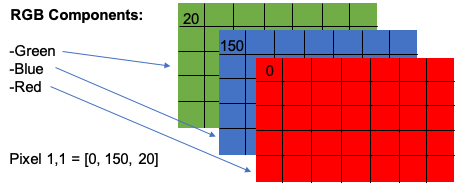
\includegraphics[width=0.9\linewidth]{figures/ch15_pixel.png}
\caption{Representation of the matrix data structure of a RGB image in which each pixel contains information for the intensity of each color component}
\label{fig:pixel}
\end{figure}

The good news when working with digital images is that the concept of \texttt{pixel} (picture element) will help you to understand the basic mathematical representation behind computational analysis of images. A rectangular grid of pixels is represented by a dot matrix which in turn generates a \texttt{bitmap image} or \texttt{raster graphic}. The dot matrix data structure is a basic but powerful representation of the images since we can conduct multiple simple and advanced operations with the matrices. Specifically, each dot in the matrix is a number that contains information about the intensity of each pixel (that commonly ranges from 0 to 255) also known as bit or color depth (figure~\ref{fig:pixel}). This means that the numerical representation of a pixel can have 256 different values being 0 the darkest tone of a given color and 255 the lightest. Keep in mind that if you divide the pixel values by 255 you will have a 0-1 scale to represent the intensity.

In a blank-and-white picture we will only have one color (grayscale), with the darker points representing the black and the lighter ones the white. The mathematical representation will be a single matrix or a two-dimensional array in which the number of rows and columns will correspond to the dimensions of the image. For instance in a 224 x 224 black-and-white picture we will have 50,176 integers (0-255 scales) representing each pixel intensity. 

In \refex{imagel} we convert our original JPG picture to grayscale and then create an object with the mathematical representation (a 453 x 805 matrix).

\pyrex[output=both,caption=Converting images to grayscale and creating a two-dimensional array]{chapter15/imagel}

By contrast, colour images will have multiple color channels that depend on the color model you chose. One standard color model is the  three-channel RGB (\textit{red}, \textit{green} and \textit{blue}), but you can find other variations in the chosen colors and the number of channels such as: RYB (\textit{red}, \textit{yellow} and \textit{blue}), RGBA (\textit{red}, \textit{green}, \textit{blue} and \textit{alpha}\footnote{Alpha refers to the opacity of each pixel} ) or CMYK (\textit{cyan}, \textit{magneta}, \textit{yellow} and \textit{key}\footnote{Key refers to \textit{black}}).  We will mostly use RGB in this book since it is the most used representation in the state-of-the-art literature in computer vision given that these color channels yield more accurate models. RGB's mathematical representation will be a three-dimensional matrix or a collection of three two-dimensional arrays (one for each color). Then a RGB 224 x 224 picture will have 50,176 pixel intensities for each of the three colors, or in other words a total of 150,528 integers!

Now, in \refex{imagergb} we convert our original JPG file to a RGB object and then create a new object with the mathematical representation (a 453 x 805 x 3 matrix).

\pyrex[output=both,caption=Converting images to RGB color model and creating three two-dimensional arrays]{chapter15/imagergb}

Instead of pixels, there are other ways to store digital images. One of them is the \textit{vector graphics}, with formats such as .ai, .eps, .svg or .drw. Differently to bitmap images, they don't have a grid of dots but a set of \textit{paths} (lines, triangles, square, curvy shapes, etc.) that have a start and end point, so simple and complex images are created with paths. The great advantage of this format is that images do not get "pixeled" when you enlarge them because the paths can easily be transformed 	while remaining smooth. However, to obtain the standard mathematical representation of images you can easily convert (back and forth) the vector graphics to raster graphics such as RGB.

Sometimes you need to convert your image to a specific size. For example, in the case of image classification this is a very important step since all the input images of the model must have the same size. For this reason, one of the most common tasks in the preprocessing stage is to change the dimensions of the image in order to adjust width and height to a different size. In \refex{resize} we use \fn{resize} function in \pkg{pil} and \fn{image\_scale} function in \pkg{imagemagik} to reduce the first of our original pictures in RGB (\texttt{my\_image1\_RGB}) to 25\% . Notice that we first obtain the original dimensions of the photograph (i.e. \texttt{my\_image1\_RGB.width} or \verb|image_info(my\_image1\_RGB)['width'][[1]]|) and then multiply by 0.25 in order to obtain the new size which is the argument required by the functions.

\pyrex[output=both,format=png,caption=Resize to 25\% and visualize a picture]{chapter15/resize}

Now, using the same functions of the latter example, we specify in \refex{resize2} how to resize the same picture to 224 x 244, which is one of the standard dimensions in computer vision. 

\pyrex[output=both,format=png,caption=Resize to 224 x 224 and visualize a picture]{chapter15/resize2}

You may have noticed that the new image has now the correct width and height but that it looks deformed. The reason is that the original picture was not squared and our order was to forcedly fit it into a 224 x 224 square, loosing its original aspect. There are different alternative to solve this issue, but probably the most extended is to \textit{crop} the original image to create a squared picture. As you can see in \refex{crop} we can create a function that first determines the orientation of the picture (vertical versus horizontal) and then cut the margins (upper and down if it is vertical; and left and right if it is vertical) to create a square. After applying this ad hoc function \fn{crop} to the original image we can resize again to obtain a non-distorted 224 x 224 image.

Of course you are loosing now part of the picture information, so you may think of other alternatives such as filling a couple of sides with blank pixels (or \texttt{padding}) in order to create the square by adding information instead of removing.

\pyrex[output=both,format=png,caption=Function to crop the image to create a square and the resize the picture]{chapter15/crop}

You can also adjust the orientation of the image, flip or flop it, or change its background, among other commands. These techniques might be useful for creating extra images in order to enlarge the training set in image classification (see xxx). This is called \textit{data augmentation} and consists for duplicating the initial examples from where the model learn and give them some twist so the algorithm can be more robust and generalize better. In \refex{crop} we used the \fn{rotate} method in \pkg{pil} and \fn{image\_rotate} function in \pkg{imagemagik} to rotate 45 degrees the above resized image \texttt{my\_image1\_RGB\_224} to see how easy we can get an alternative picture with similar information to include in an augmented training set.

\pyrex[output=both,format=png,caption=Rotating 45 degrees a picture]{chapter15/rotate}

Finally, the numerical representation of visual contents can help us to \textit{compare} pictures in order find similar or even duplicate images. Let's take the case of RGB images which in \refex{imagergb} we showed how to transform into a three two-dimensional array. If we now convert the 3D matrix of the image into a flatten vector we can use use new simpler numerical representation to estimate similarities. Specifically, as we do in \refex{flatten}, we can take the vectors two \textit{flatten images} of resized 15 x 15 images to ease computation (\texttt{img\_vect1} and \texttt{img\_vect2}) and use \textit{cosine similarity} to estimate how akin those images are. We stacked the two vectors in a matrix and then used the \fn{cosine\_similarity} function of the \fn{metrics} module of the  \pkg{sklearn} package in Python and \fn{cosine} function of the \pkg{lsa} package in R.

\pyrex[output=both,caption=Comparing two flatten vectors to detect similarities between images]{chapter15/flatten}
 
As you can notice in the resulting matrix when the images are compared with themselves (that would be the case of an exact duplicate) the obtain a value of 1. Similar images would obtain values under 1 but still close to it, while dissimilar images would obtain low values.

\section{Image classification}
\label{sec:cnn}

In this section, we will learn how to conduct computational image classification which is probably the most extended supervised machine learning application in the field of automatic analysis of images in communication and social sciences. We will firstly discuss how to apply a \textit{shallow} algorithm and then a deep-learning approach, given a labelled data set. 	

In an image classification task we train a model with examples (e.g. a corpus of pictures with labels) in order to predict the category of any given new sample. It is the same logic used in supervised text classification  explained in Section~\ref{sec:supervised} but suing images instead of texts. For example, if we show many pictures of cats and many of houses the algorithm would learn the constant features in each and will tell you with some degree of confidence if a new picture contains either a cat or a house. It is the same with letters, numbers, objects or faces, and you can apply either binary or multi-class classification. Just think when your vehicle registration plate is recognized by a camera or when your face is automatically labelled in pictures posted in Facebook.

Beyond image classification we have other specific tasks in computer vision such as \textit{object detection} or \textit{semantic segmentation}. To conduct object detection we have first to locate all the possible objects contained in a picture by predicting a bounding box (i.e. height and weight, as well as the four points corresponding to the vertical and horizontal coordinates of the center of the object), which is normally an regression task. Once the bounding boxes are placed around the objects, we must apply multi-class classification as explained earlier. In the case of semantic segmentation, instead of classifying objects, we classify each pixel of the image according to the class of the object the pixel belong to, which means that different objects of the same class might not be distinguished. Figure~\ref{fig:location} shows an example of each of these techniques presented by \citet{geron2019hands}.

\begin{figure}
\centering
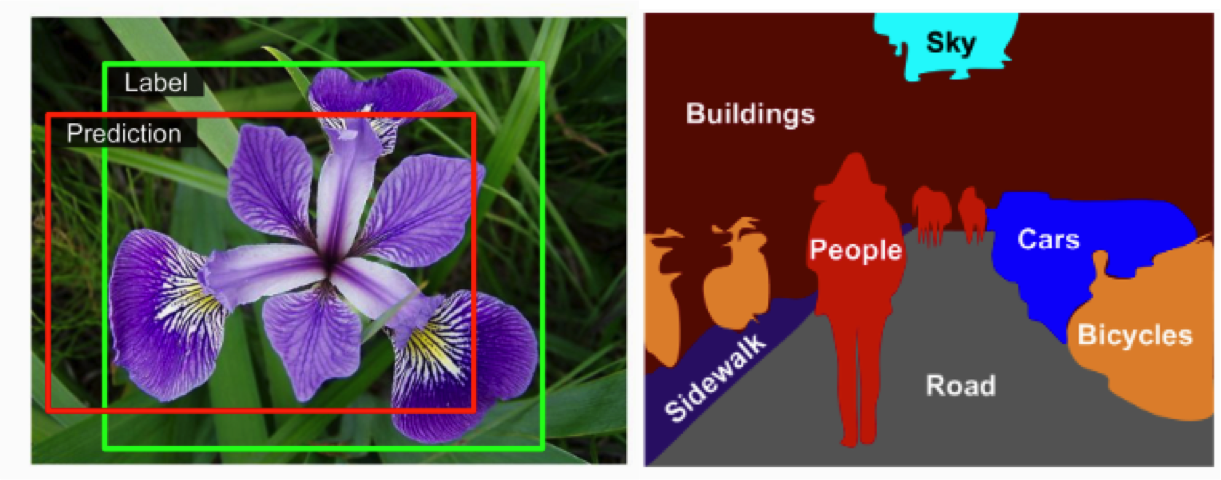
\includegraphics[width=0.9\linewidth]{figures/ch15_location.png}
\caption{Object detection (left) versus semantic segmentation (right).
Source: \citet{geron2019hands}}
\label{fig:location}
\end{figure}

It is beyond of the scope of this book to address the implementation of object detection or semantic segmentation, but we will focus on how to conduct basic image classification in state-of-the-art libraries in R and Python. As you may have imagined we will need some already-labelled images to have a proper training set. It is also out of the reach of this chapter to collect and annotate the images, which is the reason why we will mostly rely on pre-existing image databases (i.e. MINST or Fashion MINST) and pre-trained models (i.e. CNNs architectures), or will provide you with ad hoc annotated images if it is necessary. 

\subsection{Basic classification with shallow algorithms}
\label{subsec:shallow}

In Chapter~\ref{chap:introsml} we introduced you into the exciting world of machine learning and in Section~\ref{sec:supervised} we showed how to used the \textit{supervised} approach to classify texts. Most of the discussed models were based in the so called \textit{shallow} algorithms (Naïve Bayes, Regression, Support Vector Machines, Decision Trees or Random Forest), in opposition to other algorithms liked to \textit{deep} learning. As we will see in the next section, deep neural networks are nowadays the best option for complex tasks in image classification. However, we will now explain how to conduct simple multi-class classification of images that contain numbers with some shallow algorithms.

Let us begin by training a model to recognize numbers using 70,000 small images of digits handwritten from the Modified National Institute of Standards and Technology (MNIST) dataset. This popular training corpus contains gray-scale examples of numbers written by American students and workers and it is usually employed to test machine learning models (60,000 for training and 10,000 for testing). Image sizes are 28 x 28, which generates 784 features for each image, with pixels values from white to black represented by a 0-255 scales. In Figure~\ref{fig:numbers} you can observe the 

\begin{figure}
\centering
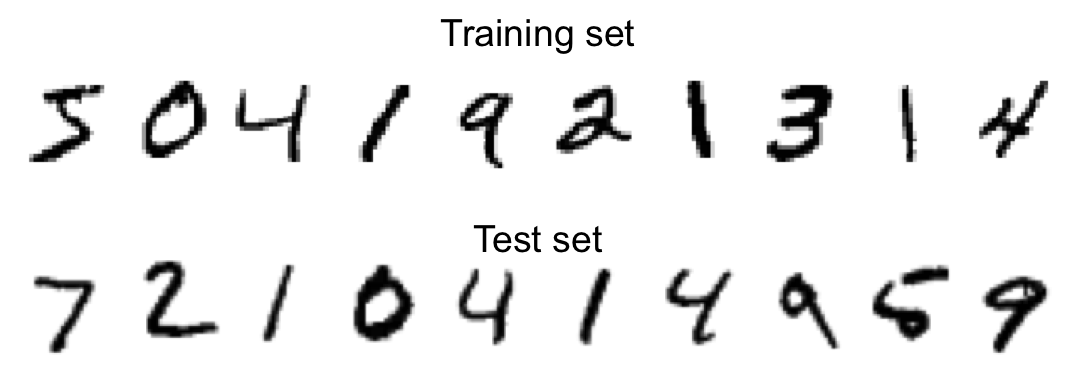
\includegraphics[width=0.9\linewidth]{figures/ch15_numbers.png}
\caption{First 10 handwritten digits from the training and test set of the MNIST}
\label{fig:numbers}
\end{figure}

In \refex{mnist} we...

\pyrex[output=both,caption=XXX]{chapter15/mnist}

And in \refex{multiclass}  we    with 100 trees ... obtain an accuracy over 0.97

\pyrex[output=both,caption=XXX]{chapter15/multiclass}



\subsection{Deep learning for image analysis}
\label{subsec:deep}

MLP for image classification p 297   Fashion MNIST (https://github.com/zalandoresearch/fashion-mnist)

\subsection{Fine tuning an open source CNN}
\label{subsec:deep}

Fine tuning an open source CNN   RestNet 18? (Andreu example)


\setcounter{chapter}{16}
\chapter{Scaling up and distributing}
\label{chap:scalingup}

\begin{abstract}
  Throughout this book, we were working with examples that consisted of
  code to conduct one specific analysis of data datasets of modest size.
  But at one point, you may want to scale up. You may want that others
  can apply your code to their data; and you may want to be able to also
  use your own analyses on larger and more complex datasets. Or you may
  need to run analyses that your own computer cannot deal with.
  This chapters deal with such  steps and point you to some techiques that become increasingly useful
  the larger your projects get.  
\end{abstract}

\keywords{databases, cloud computing, containerization, source code, version control}


\begin{objectives}
\item Be able to scale up your analyses
\item Know when to use databases
\item Know when to use cloud computing
\item Know about distributing source code and containers.
\item \ldots
\end{objectives}

\begin{feature}
In this chapter, we provide a brief overview of techniques for scaling up computational analyses. In particular, we introduces SQL and noSQL databases, cloud computing platforms, version control systems, and Docker containers.
\end{feature}


\section{Storing data in SQL and noSQL databases}
\label{sec:databases}

\subsection{When to use a database}
In this book, we have so far stored our data in files. In fact, before
covering the wide range of methods for computational analysis, we
discussed some basics of file handling
(\refchap{filetodata}). Probably, you did not experience any major
trouble here (apart from ocassional struggles with non-standard
encodings, or confusion about the delimiters in a csv file). On the
other hand, the examples we used were still modest in size: usually,
you were dealing with a handful of csv files; except from huge image classification datasets, the maximum you had to
deal with where the 50,000 text files from the IMDB movie review
dataset.

In particular, when loading your data into a dataframe, you copied all
the data from your disk into memory\footnote{In fact, this is
  sometimes a reason to avoid dataframes: for instance, it is possible
  to use a generator that reads data line-by-line from a file and
  yields them to \pkg{scikit-learn}. In this way, only \emph{one} row
  of data is in your memory at the same time (see \refsec{functions}).}
But what if we want to scale up our analyes a bit
\cite[see][]{Trilling2018b}? Maybe we want to build up a larger
datacollection, maybe even share it with multiple team members, search
and filter our data, or collect it over a larger timespan? An
example may illustrate the problems that can arise.

Imagine you do some web scraping (\refchap{scraping}) that goes beyond
a few thousand texts. Maybe you want to visit relevant news sites on a
regular basis (say, once an hour) and retrieve everything that's
new. How do you store your data then? You could append everything to a
huge csv file, but this file would quickly grow so large that you
cannot load it into memory any more. Besides, you may run the risk of
corrupting the file if something goes wrong in one of your attempts to
extend the file. Or you could also write each article to a new, separate file.
That's maybe more failsafe, but you would need to design a good way
to organize the data. In particular, devising a method to search
and find relevant files would be a whole project in itself.

Luckily, you can outsource all these problems to a database that you can
install on your own computer or possibly on a server (in that case, make
sure that it is properly secured!). In the example, the scraper, which
is running once an hour, just sends the scraped data to the database
instead of to a file, and the database will take care of storing it.
Once you want to retrieve a subset of your articles for analysis,
you can send a query to the database and read from it. Both Python and
R offer integration for multiple commonly used databases. It is even
possible to directly get the results of such a database query in
form of a dataframe.

We can distinguish two main categories of databases
that are most relevant to us \citep[see also][]{Gunther2018}:
relational databases (or SQL-databases) and noSQL-databases. Strictly
speaking, SQL (``structured query language'') is a query language for
databases, but it is so widespread that it is used almost synonymously
for relational databases. Even though they have been around for
already 50 years \citep{Codd1970}, relational databases still are very
powerful and very widely used.  They consist of multiple tables that
are linked by shared columns (keys). For instance, you could imagine a
table with the orders placed in a webshop that has a column
|customer-id|, and a different table with addresses, billing
information, and for each |customer-id|. Using filter and join
operations (like in \refchap{datawrangling}, but then on the database directly), one can then easily retrieve
information on where the order has to be shipped. A big advantage of
such a relational database is that, if a customer places 100 orders,
we do not need to store their address 100 times, but only once, which
is not only more efficient in terms of storage, but also prevents
inconsistencies in the data.

In contrast to SQL databases, noSQL databases are not based on tables,
but use concepts such as ``documents'' or key-value pairs, very much
like Python dictionaries or JSON files. These types of databases are
particularly interesting when your data are less well-structured. If
not all of your cases have the same variables, or if the content is not
well-defined (let's say, you don't know exactly in what format the date
of publication on a news site will be written), or if the data structure
may change over time, then it is hard or impossible to come up with a
good table structure for an SQL database. Therefore, in many ``big data''
contexts, noSQL databases are used, as they -- depending on your
configuration -- will happily accept almost any kind of content you dump
in them. This comes, of course, at the expense of giving up advantages
of SQL databases, such as the avoidance of inconsistencies. But often,
you may rather want to store your data first and clean up later, rather
than risking that data collection fails because you enforced a too strict
structure. Also, there are many noSQL databases that are very fast in
searching full text -- something that SQL databases, in general, are
not optimzied for.

Despite all of these differences, both SQL and noSQL databases can play
the same role in the computational analysis of communication. They both
help you to focus on data collection and data analysis without needing
to device an ingenious way to store your data. They both allow for much
more efficient searching and filtering than you could design on your own.
All of this becomes especially interesting when your dataset grows too
large to fit in memory, but also when your data are continuously changed,
for instance because new data are added while scraping.


\subsection{Choosing the right database}
Choosing the right database is not always easy, and has many consequences
for the way you may conduct your analyses. As \citet{Gunther2018} explain,
this is not a purely technical choice, but impacts your social-scientific
workflow. Do you want to enforce a specific structure from the very
start, or do you rather want to collect everything first and clean up
later? What is your tradeoff between avoiding any inconsistency and risking
to throw away too much raw information? 

Acknowledging that there are often many different valid choices, and at
the risk over oversimplifying matters, we will try to give some guidance
in which databases to choose by offering some guiding questions.


\paragraph{How is your data structured?} Ask yourself: Can I organize my data
in a set of relational tables? For instance, think of television
viewing data: There may be a table that gives information on when the
television set was switched on and which channel was watched and by
which user id. A second table can be used to associate personal
characteristics such as age and gender with the user id. And a third
table may be used to map the time stamps to details about a specific
program aired at the time.  If your data looks like this, ask
yourself: Can I determine the columns and the data types for each
column in advance?  If so, then a SQL database such as \pkg{MySQL},
\pkg{PostgreSQL}, or \pkg{MariaDB} is probably what you are looking
for. If, on the other hand, you cannot determine such a structure a
priori, if you believe that the structure of your information will
change over time, or if it is very messy, then you may need a more
flexible, noSQL approach, for instance using \pkg{MongoDB} or
\pkg{ElasticSearch}.

\paragraph{How important is full-text search for you?} SQL databases can handle numeric datatypes as well as text datatypes, but they are usually not optimized for the latter. They handle short strings (such as usernames, addresses, and so on) just fine, but if you are interested in full-text search, they are not the right tool for the job. This is in particular true if you want to be able to do fuzzy searches where, for instance, also documents containing the plural of a word that you searched for as singular are found. Databases of, for instance, news articles, tweets, transcripts of speeches, or other documents are much better accessible in a database such as \pkg{ElasticSearch}.


\paragraph{How flexible does it need to be?} In relational databases, it is relatively hard to change the structure afterwards. In contrast, a noSQL database has no problem whatsoever with adding a new document that contains keys that did not exist before. There is no assumption that all documents contain the same keys. Therefore, if it is hard to tell in advance which ``columns'' or ``keys'' may represent your data best, you should stay clear of SQL databases. In particular, if you think of gradually extending your data and use it on a long timeline for re-use, potentially even by multiple teams, the flexibility of a noSQL database may be a game changer.



\subsection{A brief example using SQLite}

Installing a database server such as \pkg{mysql}, \pkg{mariadb} (an
open-source fork of mysql), \pkg{MongoDB}, or \pkg{Elasticsearch} is
not really difficult (in fact, it may already be come pre-packaged
with your operating system), but the exact configuration and setup may
differ widely depending on your computer and your needs. Most
importantly, especially if you store sensitive data in your database,
you will need to think about authentication, roles, etc. --- all
beyond the scope of this book.

Luckily, there is a compromise between storing your data in files
that you need to manage yourself and setting up a database server,
locally or remotely. The library \pkg{SQlite} offers a self-contained
database engine -- essentially, it allows you to store a whole
database in one file and interact with it using the SQL query language.
Both R and Python offer multiple ways of directly interacting with
sqlite files (\refex{sqlite}). This gives you access to some great
functionality way: after all, you can issue (almost) any SQL command
now, including (and maybe most imporantly) commands for filtering,
joining, and aggregating data. Or you could consider immediately writing
each datapoint you get from an API or a webscraper (\refchap{scraping})
without risking to loose any data if connections time out or scraping
fails halfway.

\pyrex[input=both, output=py, format=table, caption={\pkg{SQLite} offers you database functionality without setting up a database server such as \pkg{mysql}}]{chapter17/sqlite}

Of course, \pkg{SQlite} cannot give you the same performance that a ``real'' mysql (or similar) installation could offer. Therefore, if your project grows bigger, or if you have a lot of read- or
write-operations per second, then you may have to switch at one
point. But as you can see in \refex{sqlite}, Python and R do not
really care about the backend: all you need to do is to change the
connection |conn| such that it points to your new database instead of
the sqlite file.




\section{Using cloud computing (CARLOS}
\label{sec:cloudcomputing}


\section{Publishing your source}
\label{sec:publishingsource}

Already in \refsec{practices}, we briefly introduced the idea of
version control protocols such as \concept{git}, and the most well-known
online git repostiory \concept{GitHub}.
There are others, such as \concept{Bitbucket}
and the question of which one you use is not really of importance for our
argument here. Already for small projects, it is a good idea to use
version control so that you can always go back to earlier versions,
but as soon as you start working with multiple people on one project,
it becomes indespensable.

In particular, it is possible to work on multiple \emph{branches},
different versions of the code that can later be merged again. In this
way, it is possible to develop new features without interfering with
the main version of the code. There are plenty of git tutorials
available online, and we highly recommended using git from the
beginning of a specific project on -- be it your bachelor, master or doctoral thesis, a paper, or a tool that you want to create.

In the compuational analysis of communication, it becomes more and
more the norm to publish all your source code together with an
article, even though it is important to keep in mind ethical and legal
restrictions (\cite{VanAtteveldt2019}). Using a version control
platform like github from the beginning makes this easy: when
publishing your paper, the only thing you have to do is to set access
of your repository to ``public'' (in case it was private before), add
a |README.md| file (in case you have not done so earlier), and
preferrably, get a persistenant identifier, a |doi| for your
code (see \url{https://guides.github.com/activities/citable-code/}).
And don't forget to add a license to your code, such as MIT, GPL, or
Apache. All of these have specific implications on what others can or
cannot do with your code (e.g., whether it can be used for commercial
purposes or whether derivatives need to be published under the same license as well). Whatever you choose here, it is important \emph{that} you make a choice, as otherwise, it may not be (legally) possible to use
your code at all. 
If your code pertains to a specific paper, then we suggest to organize
your repository as a so-called ``research compendium'', integrating
both your code and your data.
\cite{compendium} provide a template and tools for easily creating one%
\footnote{See url{https://compendium.ccs.amsterdam}}.

In virtually all instances, your code will rely on libraries written
by others, which are available free of charge to you. Therefore,
it only seems fair to ``give back'' and make sure that any code that
you wrote and that can be useful to others, is also available to them.

Just like in the case of a research compendium for a specific paper,
also publishing source code for more generic re-use begins with a
github repository. In fact, both R (with \pkg{devtools}) and Python
(via \pkg{pip}) can install packages directly from github. In order
to make sure that your code can be installed as a package, you
need to follow specific instructions on how to name files, how to
structure your directory, and so on (see \url{https://packaging.python.org/tutorials/packaging-projects/}
and \url{http://r-pkgs.had.co.nz/}).

Regardless of these specific technical instructions, you can make
sure from the outset, though, that your code is easily re-usable.
The checklist below can help making your code publishable from the
outset.

\begin{itemize}
\item Do not hard-code values. Rather than using |"myoutputfile.csv"| or |50| within your script, create constants like |OUTPUTFILE="myoutputfile"| and |NUMBER_OF_TOPICS=50| at the beginning of your script and use these variables instead of the values later on. Even better, let the user provide these arguments as command line arguments or via a configuration file.
\item Use functions. Rather than writing large scripts that are executed from the first line to the last in that order, structure the code in different functions that fulfill one specific task each, and can hence be reused. If you find yourself copy-pasting code, then most likely, you can write a function instead.
\item Document your code. Use docstrings (Python) or comments (R) to make clear what each function does.
\end{itemize}



\section{Distributing your software as container}
\label{sec:container}
When publishing your software, you can think of multiple user
groups. Some may be interested in building on and further developing
your code. Some may not care about your code at all and just want your
software to run. And many others will be somewhere in between.

\emph{Only} publishing your source code (\refsec{publishingsource}) may
be a burden for those who want your code to ``just run'' once your
code becomes more complex and has more dependencies. Imagine a
scenario where your software requires a specific version of
Python or R and/or some very specific (or maybe incompatible) libraries
that you do not want to force the user to install.

And maybe your prospective user does not even know any R or Python.

For such cases, so-called containers are the solution, with as most
prominent platform \pkg{Docker}. You can envision a container as a
minimalistic virtual machine that includes everything to run your
software. To the outside, none of that is visible -- just a network
port to connect to, or a command line to interact with, depending on
your choices.

Software that is containerized using docker is distributed as a
so-called \emph{docker image}. You can build such an image yourself,
but it can also be distributed by pushing it to a so-called registry,
such as the \pkg{Docker Hub}. If you publish your software this
way, the end user has to do nothing else than installing Docker and
running the command |docker run nameofyourimage| - it will be even
downloaded automatically if necessary. There are also GUI versions
of Docker available, which lowers the threshold for some end user
groups even more.

Let's illustrate the typical workflow with a toy example. Imagine
you wrote the following script, |myscript.py|:

\verb|
import numpy as np

from random import randint

a = randint(0,10)

print(f"exp({a}) = {np.exp(a)}")
|

You think that this is an awesome program (after all, it calculates
$e$ to the power of a random integer!), and others should be able
to use it. And you don't want to bother them with setting up Python,
installing numpy, and then running the script. In fact, they do
not even need to \emph{know} that it's a Python program. You
could have written it as well in R, or any other langauge -- for
the user, that will make no difference at all.

What would a docker image that runs this code need to contain? Not
much: First some basic operating system (usually, a tiny Linux distribution),
Python, numpy, and the script itself.

To create such a Docker image, you create a file named |Dockerfile|
in the same directory as your script with the following content:

\texttt{
FROM python:3

ADD myscript.py /

RUN pip install numpy

CMD [ "python", "./myscript.py" ] }


The first line tells Docker to build your new image by starting
from an existing image that already contains an operating system
and Python3. You could also start from scratch here, but this
makes your life much easier. The next line adds your script to the
image, and then we run |pip install numpy| within the image.
The last line just specifies which command with which parameters
needs to be executed when the image is run -- in our case
|python ./myscript.py|.

To create the image, you run |docker build -t dockertest .| (if
you want to name the image ``dockertest''. After that, you can run
it using |docker run dockertest| -- and, if you want to, publish it.

Easy, right?

But when does it make sense to use Docker? Not in our toy example,
of course. While the original code is only a couple of bytes, it now
got bloated to hundreds of megabytes. But there are plenty of
scenarios where this makes a lot of sense.

\begin{itemize}
\item To ``abstract away'' the inner workings of your code. Rather than giving potentially complicated instructions how to run your code, which dependencies to install, etc., you can just provide users with the Docker image, in which everything is already taken care of.
\item To ensure that users get the same results. Though it doesn't form a huge problem on a daily bases for most computational scientists, different versions of different libraries on different systems may occasionally produce slightly different results. The container ensures that the code is run using the same software setup.
\item To avoid interfering with existing installations. Already our toy example had a dependency, \pkg{numpy}, but often, dependecies can be more complex and a program we write may need very specific libraries, or even some other software beyond Python or R libraries. Distributing the source code alone means forcing the user to also install these; and there are many good reasons why people may be reluctant to do so. It may be incompatible with other software on their computer, there may be security concerns, or it just may be too much work. But if it runs inside of the docker container, many of these problems disappear.
\end{itemize}

In short, the Docker image is rarely the \emph{only} way in which you distribute your source code. But already adding a Dockerfile to your github repository so that users can build a Docker container can offer another and maybe better way of running your software to your audience.



\backmatter
% bibliography, glossary and index would go here.

\bibliography{references}%
\latexprintindex


\end{document}
